%% LyX 1.5.2 created this file.  For more info, see http://www.lyx.org/.
%% Do not edit unless you really know what you are doing.
\documentclass[12pt,a4paper,english]{report}
\usepackage{mathptmx}
\usepackage[T1]{fontenc}
\usepackage[latin9]{inputenc}
\setcounter{secnumdepth}{3}
\setcounter{tocdepth}{3}
\usepackage{array}
\usepackage{subfigure}
\usepackage{nicefrac}
\usepackage{amsmath}
\usepackage{graphicx}

\makeatletter

%%%%%%%%%%%%%%%%%%%%%%%%%%%%%% LyX specific LaTeX commands.
%% Because html converters don't know tabularnewline
\providecommand{\tabularnewline}{\\}

%%%%%%%%%%%%%%%%%%%%%%%%%%%%%% Textclass specific LaTeX commands.
\newcommand{\lyxaddress}[1]{
\par {\raggedright #1
\vspace{1.4em}
\noindent\par}
}

%%%%%%%%%%%%%%%%%%%%%%%%%%%%%% User specified LaTeX commands.
\usepackage{longtable}
\baselineskip=18pt
\textwidth 5.5in
\textheight 8.5in
\setlength{\oddsidemargin}{0.0in}
\setlength{\evensidemargin}{0.0in}

\usepackage{babel}
\makeatother

\begin{document}

\title{\textbf{General Utility Lattice Program}}
\begin{center}
\textbf{\huge General Utility Lattice Program}
\par\end{center}
\begin{center}
\textbf{\large Version 6.2}
\par\end{center}
\author{\textbf{\textsl{Julian D. Gale}}}
\begin{center}
\textbf{\large Julian D. Gale}
\par\end{center}
\lyxaddress{\begin{center}
\textbf{Curtin Institute for Computation,}

\textbf{School of Molecular and Life Sciences,}

\textbf{Curtin University, }

\textbf{P.O. Box U1987, Perth, WA 6845,}

\textbf{Australia}

\textbf{email: gulpcode@curtin.edu.au} 
\par\end{center}}

\chapter{Introduction \& background}

The General Utility Lattice Program (GULP) is designed to perform
a variety of tasks based on force field methods. The original code
was written to facilitate the fitting of interatomic potentials to
both energy surfaces and empirical data. However, it has expanded
now to be a general purpose code for the modelling of condensed phase
problems. While version 1.0 focussed on solids, clusters and embedded
defects, the latest version is also capable of handling surfaces,
interfaces, and polymers. 

As with any large computer program (and GULP currently runs to about
750,000 lines) there is always the possibility of bugs. While every
attempt is made to ensure that there aren't any and to trap incorrect
input there can be no guarantee that a user won't find some way of
breaking the program. So it is important to be vigilant and to think
about your answers - remember GIGO! Immature optimising compilers
can also be a common source of grief. As with most programs, the author
accepts no liability for any errors but will attempt to correct any
that are reported. 

As from GULP3.4, the program has migrated to Fortran 90 (including subsequently some
features from later standards). From version 4.0 the code
included several major additions, the most significant of which are the
addition of the ReaxFF reactive force field and also the facility to use
continuum dielectric solvation in multiple dimensions through the 
COSMIC algorithm, derived as the name would suggest from COSMO.
A further major improvement is the addition of a stochastic thermostat/barostat
with a new integrator in molecular dynamics. This is far more robust than the
old schemes used and less sensitive to the choice of parameters.
Finally, the ability to calculate PDF data has been added courtesy of 
Beth Cope and Martin Dove (University of Cambridge at the time; now
Queen Mary, University of London). In version 4.2 the calculation of
thermal conductivity has been added based on the Allen-Feldman
approach for diffusons. This was achieved through a collaboration
with Jason Larkin (Carnegie Mellon, Pittsburgh). 

For GULP5.0 onwards the major change is the parallelisation of second
derivatives with distributed memory. This allows much large problems to 
be tackled where full second or even third derivatives are needed, such
as phonon calculations and free energy minimisation. Because this 
represents a major change in the code not all features are currently 
enabled with parallel second derivatives. Currently the main restrictions
are that partial occupancies, variable charges and the breathing shell model are not yet
available in this mode. However, these restrictions will be removed in future
versions.

In GULP5.1 there have been several additions. Split bond charge equilibration 
has been added, along with multiple charge ranges for electronegativity parameters.
This allows the MEAM\_2NN\_QEq method to be used. An interface to the 
code Alamode (https://alamode.readthedocs.io/en/latest/intro.html) has been added that automates the calculation of the thermal 
conductivity using the Boltzmann Transport Equations based on third order force
constants. 

For GULP6.0 the major change to the code is that rigid molecules are now included.
At present rigid molecules can be used in optimisation, property and phonon calculations
for bulk systems of all periodicities. Defect calculations and molecular dynamics do not
currently support rigid molecules, but this should be remedied in future releases. Methods
that require third derivatives are also not currently available, as analytic derivatives of 
rigid molecules are only implemented to second order. 

For GULP6.1 the universal force field of Spicher and Grimme, GFN-FF \cite{GFNFF}, has been added 
with the extension to periodic boundary conditions, pGFN-FF. \cite{pGFNFF}. Also added is support for 
valence bond force fields. 

For GULP6.2 the major change is the addition of analytic second derivatives and phonons for ReaxFF.
In addition, the calculation of charges using extended Huckel theory has been added for s and p block elements, which
allows the use of the AA-CLP force field of Gavezzotti. Properties for variable charge models are now computed with charge derivatives including those for electric fields.

\section{References for GULP}

The following papers describe various aspects of GULP:

\paragraph{Basic algorithms and symmetry adaption:}

\begin{itemize}
\item J.D. Gale, J.C.S. Faraday Transactions, 93, 629-637 (1997)
\end{itemize}

\paragraph{Detailed background theory:}

\begin{itemize}
\item J.D. Gale and A.L. Rohl, Molecular Simulation, 29, 291-341 (2003)
\end{itemize}

\paragraph{Free energy minimisation:}

\begin{itemize}
\item J.D. Gale, J. Phys. Chem. B, 102, 5423 (1998)
\end{itemize}

\paragraph{Review of status and functionality:}

\begin{itemize}
\item J.D. Gale, Z. Krist., 220, 552-554 (2005)
\end{itemize}

\paragraph{Solvent models in GULP:}

\begin{itemize}
\item J.D. Gale and A.L. Rohl, Molecular Simulation, 33, 1237-1246 (2007)
\end{itemize}

\paragraph{ReaxFF in GULP:}

\begin{itemize}
\item J.D. Gale, P. Raiteri and A.C.T. van Duin, PCCP, 13, 16666-16679 (2011)
\end{itemize}

\paragraph{pGFNFF in GULP:}

\begin{itemize}
\item J.D. Gale, L. Leblanc, P.R. Spackman, A. Silvestri and P. Raiteri, J. Chem. Theory Comput., 17, 7827-7849 (2021)
\end{itemize}

\paragraph{Pair Distribution Functions in GULP:}

\begin{itemize}
\item E.R. Cope and M.T. Dove, J. Appl. Cryst., 40, 589-594 (2007)
\end{itemize}

\paragraph{Thermal conductivity in GULP:}

\begin{itemize}
\item J.M. Larkin and A.J.H. McGaughey, Phys. Rev. B, 89, 144303 (2014)
\end{itemize}


\section{Overview of program}

The following is intended to act as a brief summary of the capabilities
of GULP to enable you to decide whether your required task can be
performed without having to read the whole manual. Alternatively it
may suggest some new possibilities for calculations!


\paragraph{System types}

\begin{itemize}
\item 0-D (clusters and embedded defects)
\item 1-D (polymers, screw dislocations)
\item 2-D (slabs, surfaces, grain boundaries, interfaces)
\item 3-D (bulk materials)
\end{itemize}

\paragraph{Energy minimisation}

\begin{itemize}
\item constant pressure / constant volume / unit cell only / isotropic / orthorhombic 
\item thermal/optical calculations 
\item application of external isotropic or anisotropic pressure 
\item user specification of degrees of freedom for relaxation 
\item relaxation of spherical region about a given ion or point 
\item symmetry constrained relaxation 
\item unconstrained relaxation 
\item constraints for fractional coordinates and cell strains 
\item rigid molecule optimisation with quarternions 
\item Newton/Raphson, conjugate gradients or Rational Function optimisers 
\item BFGS or DFP updating of hessian 
\item limited memory variant of BFGS for large systems
\item search for minima by genetic algorithms with simulated annealing 
\item free energy minimisation with analytic first derivatives using quantised or classical vibrations
\item choice of regular or domain decomposition algorithms for first derivatives
\item minimisation of gradient/force norm instead of energy
\item uniaxial stress 
\item finite strain derivatives relative to a reference structure
\end{itemize}

\paragraph{Transition states}

\begin{itemize}
\item location of $n$-th order stationary points 
\item mode following 
\end{itemize}

\paragraph{Crystal properties}

\begin{itemize}
\item elastic constants 
\item bulk modulus (Reuss/Voigt/Hill conventions)
\item shear modulus (Reuss/Voigt/Hill conventions)
\item Young's modulus 
\item Poisson ratios 
\item compressibility
\item piezoelectric stress and strain constants 
\item static dielectric constants 
\item high frequency dielectric constants 
\item frequency dependent dielectric constants
\item static refractive indices 
\item high frequency refractive indices 
\item NMR chemical shifts
\item stress tensor
\item phonon frequencies 
\item phonon densities of states (total and projected) 
\item phonon dispersion curves 
\item group velocities
\item S/P-wave velocities
\item Born effective charges
\item zero point vibrational energies 
\item heat capacity (constant volume) 
\item entropy (constant volume) 
\item Helmholtz free energy 
\item pair distribution function (PDF) calculation
\item Grueneisen parameters
\item group velocities
\item thermal conductivity (Allen-Feldman model)
\item thermal conductivity (output of files for Alamode to use Boltzmann Transport Equations)
\item Raman susceptibility tensors
\item phonon mean-squared displacements
\end{itemize}

\paragraph{Molecular properties}

\begin{itemize}
\item centre of mass 
\item moment of inertia tensor
\item rotational partition function
\item translational partition function
\item rotational/translational free energy
\item Eckart purification of vibrational modes
\end{itemize}

\paragraph{Defect calculations}

\begin{itemize}
\item vacancies, interstitials and impurities can be treated 
\item explicit relaxation of region 1 
\item implicit relaxation energy for region 2 
\item energy minimisation and transition state calculations are possible 
\item defect frequencies can be calculated (assuming no coupling with 2a) 
\end{itemize}

\paragraph{Surface calculations}

\begin{itemize}
\item calculation of surface and attachment energies
\item multiple regions allowed with control over rigid or unconstrained
movement
\item can be used to simulate grain boundaries and interfaces
\item calculation of phonons allowed for region 1
\item continuum solvation of surfaces
\end{itemize}

\paragraph{Fitting}

\begin{itemize}
\item empirical fitting to structures, energies and most crystal properties
\item fit to multiple structures simultaneously 
\item simultaneous relaxation of shell coordinates during fitting 
\item fit to structures by either minimising gradients or displacements 
\item variation of potential parameters, charges and core/shell charge splits 
\item constraints available for fitted parameters 
\item simplex or BFGS minimisation algorithms for fitting
\item generate initial parameter sets by the genetic algorithm for subsequent
refinement 
\item fit to quantum mechanically derived energy hypersurfaces 
\item bond lengths, bond angles, volume and reaction energies now available as observables
\end{itemize}

\paragraph{Structure analysis}

\begin{itemize}
\item calculate bond lengths/distances 
\item calculate bond angles 
\item calculate torsion angles 
\item calculate improper torsion angles 
\item calculate out of plane distances 
\item calculation of the density and cell volume 
\item electrostatic site potentials 
\item electric field gradients 
\end{itemize}

\paragraph{Structure manipulation}

\begin{itemize}
\item convert centred cell to primitive form 
\item creation of supercells 
\item rotation of frame based on moment of inertia tensor
\item twisting of 1-D periodic structures about repeat direction
\end{itemize}

\paragraph{Charge calculation}

\begin{itemize}
\item use electronegativity equalisation method (EEM) to calculate charges for systems containing H, C, N, O, F,
Al, Si, P 
\item use QEq to calculate charges for any element 
\item new modified scheme for hydrogen within QEq that has correct forces 
\item Gasteiger charge calculation based on bond increments
\item calculation of charges from ReaxFF
\item use split bond charges for EEM
\item extended Huckel theory calculation of charges for sp block elements including periodic systems
\end{itemize}

\paragraph{Generation of files for other programs}

\begin{itemize}
\item GDIS (.gin/.res)
\item THBREL/THBPHON/CASCADE (.thb) 
\item MARVIN (.mvn) 
\item Insight (.xtl file) 
\item Insight (.arc/.car files) 
\item G-Vis (.xr) 
\item Cerius2 (.arc/.xtl/.cssr) 
\item Materials Studio
\item COSMO solvent accessible surface for Materials Studio
\item SIESTA (.fdf)
\item Molden (.xyz)
\item QMPOT (.frc)
\item General (.cif/.xml)
\item DLV (.str)
\item Alamode files (for calculation of thermal conductivity using Boltzmann Transport Equations)
\item lammps\_pot (Table of potentials for use in LAMMPS)
\end{itemize}

\paragraph{Output files for post-processing}

\begin{itemize}
\item Pressure tensor (.pre)
\item Oscillator strengths
\item Pair distribution function (.pdf) 
\item Charges and bond orders (.qbo)
\item MD trajectory file (.trg)
\end{itemize}

\paragraph{Interatomic potentials available}

\begin{itemize}
\item pGFN-FF force field
\item Buckingham 
\item Four-range Buckingham 
\item Buckingham in MM3 format
\item Lennard-Jones (with input as A and B) 
\item Lennard-Jones (with input in $\varepsilon$ and $\sigma$ format) 
\item Lennard-Jones (with ESFF combination rules) 
\item Morse potential (with or without Coulomb subtract) 
\item Harmonic (with or without Coulomb subtract) 
\item MM3 bond stretching potential (with or without Coulomb subtract) 
\item General potential (Del Re) with energy and gradient shifts 
\item Spline 
\item Spring (core-shell) 
\item Spring with cosh functional form
\item Coulomb subtract 
\item Coulomb with erfc 
\item Coulomb with short range taper 
\item Inverse Gaussian 
\item Damped dispersion (Tang-Toennies) 
\item Rydberg potential 
\item Covalent exponential form 
\item Breathing shell harmonic
\item Breathing shell exponential
\item Coulomb with complementary error function
\item Coulomb with short range taper
\item Covalent-exponential
\item Fermi-Dirac form
\item Three body potentials - harmonic with or without exponential decay 
\item Exponential three-body potential 
\item Urey-Bradley three-body potential 
\item Stillinger-Weber two- and three-body potentials 
\item Stillinger-Weber with charge softening
\item Axilrod-Teller potential 
\item Four-body torsional potential 
\item Ryckaert-Bellemans cosine expansion for torsional potential 
\item Out of plane distance potential 
\item Tsuneyuki Coulomb correction potential
\item Squared harmonic
\item Mei-Davenport twobody
\item Glue potential
\item Short range potentials based on (complementary) error functions
\item Embedded atom method for metals (Sutton-Chen potentials and others) 
\item Modified Embedded Atom Method of Baskes and co-workers
\item Two-body potentials can be intra- or inter-molecular, or both 
\item Two-body potentials can be tapered to zero using cosine, polynomial
or Voter forms
\item Universal force field functional forms for three-, four-body cases
and out of plane
\item Universal force field combination rules available
\item Angle-angle cross out of plane potential
\item Lennard-Jones potential between atoms and a plane
\item Radial force between all atoms and a point in space
\item Sixbody out of plane - out of plane cross potentials
\item Grimme C6 damped dispersion
\item Environmentally Dependent Interatomic Potential (EDIP)
\item ReaxFF 
\item Central Force Model (CFM) potentials
\item Baskes twobody potential
\item Ziegler-Biersack-Littmark (ZBL) potential
\item Torsion potentials can be specified as improper
\item Externally defined potentials via OpenKIM version 2
\item Constant potentials for 2 and 3 body interactions for use in Ising models
\item AA-CLP force field of Gavezzotti
\end{itemize}

\paragraph{Coulomb summations}

\begin{itemize}
\item Ewald sum for 3-D
\item Parry sum for 2-D
\item Saunders et al sum for 1-D
\item Cell multipole method for 0-D
\item Wolf et al sum for 0-,1-,2-, \& 3-D
\item Smooth Particle Mesh Ewald for 3-D (energy and first derivatives only)
\end{itemize}

\paragraph{Molecular dynamics}

\begin{itemize}
\item Shell model (dipolar and breathing) molecular dynamics 
\item Finite mass or adiabatic algorithms 
\item Forward extrapolation of shells added for adiabatic algorithms
\item NVE or NVT (Fixed cell) or NPT (Variable cell shape) 
\item Stochastic integrator with thermostat/barostat
\item isotropic or orthorhombic cell constraints
\item Atom-based potential energy decomposition and forces added to trajectory file
\end{itemize}

\paragraph{Monte Carlo}

\begin{itemize}
\item Rigid molecules allowed for
\item Displacement or rotation of species
\item NVT or Grand Canonical ensembles allowed
\item Particle swaps (single or multiple) allowed
\end{itemize}

\section{Introduction}

The simulation of ionic materials has a long history going back over
most of the last century. It began with lattice energy calculations
based on experimental crystal structures through the use of Madelung's
constant. This was then expanded through the inclusion
of short-range repulsive interactions, as found in the work of Born-Lande
and Born-Mayer \cite{bornmayer}, in order that the crystal structure
be a minimum with respect to isotropic expansion or compression. For
many simple ionic materials a reasonable estimate of the lattice energy
may even be obtained without knowledge of the structure, as demonstrated
by the work of Kapustinskii \cite{kapustinskii}. Over the last few
decades atomistic simulation, in which we are only concerned with
atoms, rather than electrons and sub-atomic particles, has developed
significantly with the widespread use of computers. Correspondingly
the field has evolved from one that was initially concerned with reproducing
experimental numbers, to one where predictions are being made, and
insight is being offered.

The widespread use of atomistic simulation for solid state materials
clearly resulted from the availability of computer programs for the
task, just as much as the advent of the hardware to run the calculations.
In the early days of solid state forcefield simulation for ionic materials
much of the work in the UK was centred around the Atomic Energy Authority
at Harwell. Consequently a number of computer codes arose from this
work, such as HADES \cite{hades}, MIDAS \cite{key-118}, PLUTO \cite{pluto},
METAPOCS and CASCADE \cite{cascade}. Eventually these migrated into
the academic domain, leading to the THB suite of codes, including
THBREL, THBFIT and THBPHON from Leslie. Further development of these
programs led to the PARAPOCS code from Parker and co-workers \cite{key-91},
for free energy minimisation of solids using numerical derivatives,
and the DMAREL code from the group of Price for the simulation of
molecular crystals through the use of distributed multipoles \cite{key-105}.
There were also several other prominent codes developed contemporaneously
to the above family, in particular the WMIN code of Busing \cite{key-82},
the PCK series of programs from Williams \cite{key-83}, and the UNISOFT
program of Eckold \textit{et al} \cite{UNISOFT}. While the codes
mentioned above focus specifically on static lattice and quasiharmonic
approaches to simulation, it should not be forgotten that there was
a much larger, parallel, development of forcefield software for performing
molecular dynamics simulation leading to programs such as GROMOS \cite{gromos},
AMBER \cite{amber}, CHARMM \cite{CHARMM}, and DL\_POLY \cite{DLPOLY2,DLPOLY},
to name but a few.

This article focuses on the General Utility Lattice Program which
began development in the early 90's, and is therefore subsequent to
much of the aforemention software, but implements many of the same
ideas. However, there are increasingly many new, and unique, developments
as well. The key philosophy was to try to bring together many of the
facilities required for solid state simulation, with particular emphasis
on static lattice/lattice dynamical methods, in a single package,
and to try to make it as easy to use as possible. Of course, this
is an aim and the degree of success depends on the perspective of
the end user! It is important to also mention here the programs METADISE
from Parker and co-workers\cite{metadise}, and SHELL from the group
of Allan \cite{key-130}, which are also contemporary simulation codes
sharing some of the same ideas. 

In this work, the specific aim is to document the background to many of the features available in GULP 
and provide an introduction to the important keywords and options available.


\section{Methods}

The starting point for the majority simulation techniques is the calculation
of the energy, and so will it be for this article. Most methods are
based around the initial determination of the internal energy, with
subsequent treatment of the nuclear degrees of freedom in order to
determine the appropriate free energy to the ensemble of interest.
In principle, the internal energy of a solid is a many-body quantity
that explicitly depends upon the positions and momenta of all electrons
and nuclei. However, this is an intractable problem to solve at any
level of theory, and thus approximations must be made to simplify
the situation. To tackle this we assume that the effect of the electrons
will largely be subsumed into an effective atom, and that the energy
can be decomposed into an expansion in terms of interactions between
different subsets of the total number of atoms, $N$:

\[
U=\sum_{i=1}^{N}U_{i}+\frac{1}{2}\sum_{i=1}^{N}\sum_{j=1}^{N}U_{ij}+\frac{1}{6}\sum_{i=1}^{N}\sum_{j=1}^{N}\sum_{k=1}^{N}U_{ijk}+....\]
 where the first term represents the self energies of the atoms, the
second the pairwise interaction, etc. This decomposition is exact
if performed to a high enough order. However, we know that the contribution
from higher order terms becomes progressively smaller for most systems,
and so we choose to neglect the terms beyond a certain point and introduce
a degree of parameterisation of the remaining terms to compensate.
Justification for this is forthcoming from quantum mechanics. It is
well known that the Hartree-Fock method is a reasonable first approximation
for the description of many systems, albeit with a systematic quantitative
error for most observables. Here the highest term included is a four-centre
integral, which indicates that including up to four-body terms should
be reasonable approach, which is indeed found to be the case for most
organic systems, for example. Furthermore, it is intuitively obvious
that the further apart two atoms are, the weaker their interaction
will be. Thus the introduction of distance cut-offs is a natural way
to simplify the computational task.

The form of the explicit interaction between atoms is usually chosen
based on physical insights as to the nature of the forces between
the particles. For instance, if considering a covalent diatomic molecule
the natural representation of the potential energy surface would be
a Morse potential since this is harmonic at the minimum and leads
to dissociation at large bond lengths, in accord with spectroscopic
observation. In the following sections we will review some of the
common types of potential that are widely used, as well as some novel
approaches which point towards the future of forcefield methods.


\subsection{Coulomb interaction}

When considering ionic materials, the Coulomb interaction is by far
the dominant term and can represent, typically, up to 90\% of the
total energy. Despite having the simplist form, just being given by
Coulomb's law;\[
U_{ij}^{Coulomb}=\frac{q_{i}q_{j}e^{2}}{4\pi\epsilon_{0}r_{ij}}\]
 it is in fact the most complicated to evaluate for periodic systems
(subsequently atomic units will be employed and the factors of $4\pi\epsilon_{0}$
and $e^{2}$ will be omitted). This is because the Coulomb energy is given by a
conditionally convergent series, i.e. the Coulomb energy is ill-defined
for an infinite 3-D material unless certain additional conditions
are specified. The reason for this can be readily understood - the
interaction between ions decays as the inverse power of $r$, but
the number of interacting ions increases with the surface area of
a sphere, which is given by $4\pi r^{2}$. Hence, the energy density
of interaction increases with distance, rather than decaying. One
solution to the problem, proposed by Evjen \cite{Evjen}, is to sum
over charge-neutral groups of atoms. However, by far the most widely
employed approach is the method of Ewald \cite{key-80} for three-dimensional
materials. Here the conditions of charge neutrality and zero dipole
moment are imposed to yield a convergent series with a well-defined
limit. To accelerate the evaluation, the Coulomb term is subjected
to a Laplace transformation and then separated into two components,
one of which is rapidly convergent in real space, and a second which
decays quickly in reciprocal space. Conceptually, this approach can
be viewed as adding and subtracting a Gaussian charge distribution
centred about each ion \cite{tosi}. The resulting expressions for
real and reciprocal space, as well as the self-energy of the ion,
are given below:\[
U^{real}=\frac{1}{2}\sum_{i=1}^{N}\sum_{j=1}^{N}\frac{q_{i}q_{j}}{r_{ij}}erfc\left(\eta^{\frac{1}{2}}r_{ij}\right)\]
\[
U^{recip}=\frac{1}{2}\sum_{i=1}^{N}\sum_{j=1}^{N}\sum_{G}\frac{4\pi}{V}q_{i}q_{j}\exp\left(iG.r_{ij}\right)\frac{\exp\left(-\frac{G^{2}}{4\eta}\right)}{G^{2}}\]
\[
U^{self}=-\sum_{i=1}^{N}q_{i}^{2}\left(\frac{\eta}{\pi}\right)^{\frac{1}{2}}\]
\[
U^{electrostatic}=U^{real}+U^{recip}+U^{self}\]
Here $q$ is the charge on an ion, $G$ is a reciprocal lattice vector
(where the special case $G=0$ is excluded), $V$ is the volume of
the unit cell, and $\eta$ is a parameter that controls the division
of work between real and reciprocal space. It should also be noted
that although the reciprocal space term is written as a two-body interaction
over pairs of atoms, it can be rewritten as a single sum over ions
for more efficient evaluation. The above still leaves open the choice
of cut-off radii for real and reciprocal space. One approach to defining
these in a consistent fashion is to minimise the total number of terms
to be evaluated in both series for a given specified accuracy, $A$
\cite{key-81}. This leads to the following expressions:\[
\eta_{opt}=\left(\frac{Nw\pi^{3}}{V^{2}}\right)^{\frac{1}{3}}\]
\[
r_{max}=\left(\frac{-\ln\left(A\right)}{\eta}\right)^{\frac{1}{2}}\]
\[
G_{max}=2\eta^{\frac{1}{2}}\left(-\ln\left(A\right)\right)^{\frac{1}{2}}\]
Note that the above expressions contain one difference from the original
derivation, in that a weight parameter, $w$, has been included that
represents the relative computational expense of calculating a term
in real and reciprocal space. Tuning of this parameter can lead to
significant benefits for large systems. There have been several modifications
proposed for the basic Ewald summation that accelerate its evaluation
for large systems, most notably the particle-mesh \cite{key-112},
and fast multipole methods \cite{key-113,key-114}. Furthermore, there
are competitive approaches that operate purely in real space for large
unit cells and that scale linearly with increasing size, such as the
hierarchical fast multipole methods, though care must be taken to
obtain the same limiting result by imposing the zero dipole requirement.
This latter approach can also be applied to accelerating the calculation
of the Coulomb energy of finite clusters.

In principle, it is possible to calculate the Coulomb energy of a
system with a net dipole, $\mu$, as well. The nature of the correction
to the Ewald energy can be determined as a function of the shape of
the crystal, and the formula below can also be employed \cite{key-84}:\[
U^{dipole}=\frac{2\pi}{(2\epsilon_{r} + 1)V}\mu^{2}\]
However, the complication of using the above correction is that it
depends on the macroscopic dipole of the crystal, and even on any
compensating electric field due to the environment surrounding the
particle. Hence the dipole moment is usually ill-defined, since it
depends on the surfaces, as well as the bulk material. Even if we
neglect surface effects, the definition of the dipole moment is ambiguous
since the operator is not invariant under translation of atomic images
by a lattice vector. Consequently, we will take the Ewald result as
being definitive.

Similarly, it is possible to relax the charge neutrality constraint,
and to perform calculations on charged supercells \cite{chargedunitcell:L&G},
provided care is taken when constructing thermodynamic cycles. This
is often used when probing defect energetics as an alternative to
the Mott-Littleton method. Here the net charge, $Q$ $\left(Q=\sum q_{i}\right)$
is neutralised by a uniform background charge, leading to an energy
correction of:\[
U^{background}=-\frac{\pi}{2V\eta}Q^{2}\]
It should be noted that this correction ensures that a consistent Ewald
sum energy is computed regardless of the value of eta. However, to
correct the energy to the limit of no net interaction between the charged
cells (and therefore no cell stress) requires the addition of a positive
Madelung correction. For the special case of a simple cubic lattice, 
the correction is given by:\[
U^{madelung}=\frac{2.837297}{2a\epsilon}Q^{2}\]
Here the value 2.837297 is the Madelung constant, $a$ is the cell length and
$\epsilon$ is the dielectric constant. The general situation is more complex
and therefore only the simple cubic case correction can be automatically 
added at present. 

As the size of a system increases then the cost of evaluating the reciprocal 
space part of the Ewald sum can become potentially a bottleneck. One alternative
to the standard Ewald sum is to use the Smooth Particle Mesh Ewald (SPME) approach.
Here the reciprocal space contribution is handled by mapping the charge density onto a
grid of points in real space and then using Fourier transforms to convert to reciprocal 
space in order to evaluate the energy. A second Fourier transform is required in order
to evaluate the forces in real space. Interpolation between the grid points and the atomic
positions is performed using B-splines. The mathematical detail can be found in the 
original article \cite{SPME}. The precision of the SPME calculation is control by both 
the order of the B-splines and the grid size used, where higher values are better in 
both cases. Typically 8th order B-splines are used in GULP and the order has to be
high enough to allow differentiation to first order. The grid size is specific to the unit
cell being employed by the user and so it is important to test the convergence of the
forces with respect to this choice. In order to obtain the best performance it is important
to experiment with the use of either the rspeed or ewaldrealradius options that change
the balance between real and reciprocal space, as well as the grid size, to find the best
compromise between speed and precision. Often a good approach is to set the real 
space cut-off radius to be less than or equal to the twobody potential cutoff (especially
if this allows the use of the spatial keyword to make things more efficient) and then tune
the reciprocal space settings. 

So far we have only considered how to handle infinite 3-D solids,
but the same issues exist for lower dimensionalities. Again for a
2-D slab, the Coulomb sum is only conditionally convergent and so
an analogous approach to the Ewald sum is usually taken, originally
devised by Parry \cite{key-116,key-117}. Here the slab, or surface,
is taken so as to be oriented with the surface vectors in the $xy$
plane and with the surface normal lying parallel to $z$. The energy
contributions in real and reciprocal space are given by:\[
U^{real}=\frac{1}{2}\sum_{i=1}^{N}\sum_{j=1}^{N}\frac{q_{i}q_{j}}{r_{ij}}erfc\left(\eta^{\frac{1}{2}}r_{ij}\right)\]
\[
U_{1}^{recip}=\frac{1}{2}\sum_{i=1}^{N}\sum_{j=1}^{N}\sum_{G}\frac{\pi}{A}\frac{q_{i}q_{j}\exp\left(iG.r_{ij}\right)}{\left|G\right|}\left[\exp\left(\left|G\right|z_{ij}\right)erfc\left(\frac{\left|G\right|}{2\eta^{\frac{1}{2}}}+\eta^{\frac{1}{2}}z_{ij}\right)+\right.\]
\[
\left.\exp\left(-\left|G\right|z_{ij}\right)erfc\left(\frac{\left|G\right|}{2\eta^{\frac{1}{2}}}-\eta^{\frac{1}{2}}z_{ij}\right)\right]\]
\[
U_{2}^{recip}=-\frac{1}{2}\sum_{i=1}^{N}\sum_{j=1}^{N}\frac{2\pi q_{i}q_{j}}{A}\left[z_{ij}.erf\left(\eta^{\frac{1}{2}}z_{ij}\right)+\frac{\exp\left(-\eta z_{ij}^{2}\right)}{\left(\pi\eta\right)^{\frac{1}{2}}}\right]\]
\[
U^{self}=-\sum_{i=1}^{N}q_{i}^{2}\left(\frac{\eta}{\pi}\right)^{\frac{1}{2}}\]
Note, there are now two terms in reciprocal space involving the 2-D
reciprocal lattice vector, $G$, and here $A$ is the surface area
of the repeat unit, while $z_{ij}$ is the component of the distance
between two ions parallel to the surface normal. Again it is possible
to relax the dipolar and charge neutrality constraints within the
repeat directions. However, the approach to correcting the energy
is far more uncertain, and it is necessary to make approximations
\cite{ChargedSurfaces}. As per the 3-D case, the optimum value of
the convergence parameter can also be determined \cite{optimal2Deta}:\[
\eta_{opt}=\frac{\pi w}{A}\]
Recently, another approach has been proposed for the calculation of
the 2-D Coulomb sum, which is reported to be faster than the Parry
method for all cases, and especially beneficial as the number of atoms
increases \cite{Accelerated2Dsum}. 

Lowering the dimensionality further, we arrive at 1-D periodic systems
which represents a single polymer strand, for example. At this dimensionality
the Coulomb sum becomes absolutely convergent, though at a very slow
rate when performed directly in real space. Summing over charge neutral
units accelerates the process, though convergence is still somewhat
tardy. While there have been several proposed approaches to accelerating
the Coulomb sum, we find that the method proposed by Saunders \textit{et
al} \cite{key-108}, in which a neutralising background charge is
applied, is effective. Here there are three contributions to the energy
given by:\[
U_{1}^{real}=\frac{1}{2}\sum_{m=-M}^{+M}\sum_{i=1}^{N}\sum_{j=1}^{N}\frac{q_{i}q_{j}}{r_{ij}+ma}\]
\[
U_{2}^{real}=-\frac{1}{2}\sum_{i=1}^{N}\sum_{j=1}^{N}\frac{q_{i}q_{j}}{a}\left[\ln\left(\sqrt{\left(u+x\right)^{2}+y^{2}+z^{2}}+u+x\right)+\right.\]
\[
\left.\ln\left(\sqrt{\left(u-x\right)^{2}+y^{2}+z^{2}}+u-x\right)-2\ln a\right]\]
\[
U_{3}^{real}=\frac{1}{2}\sum_{i=1}^{N}\sum_{j=1}^{N}q_{i}q_{j}\left[\xi\left(M,r_{ij}\right)+\xi\left(M,-r_{ij}\right)\right]\]
where the first term is summed over all images of $i$ and $j$ in
the unit cells from $-M$ to $M$, $a$ is the 1-D repeat parameter
in the $x$ direction, and the remaining variables and functions are
defined as below:\[
u=a\left(M+\frac{1}{2}\right)\]
\[
\xi\left(M,r_{ij}\right)=-\sum_{i=1}^{M}E_{i}a^{2i-1}W_{2i-1}\left(u+x,y^{2}+z^{2}\right)\]
\[
W_{n}\left(u+x,\alpha\right)=\left(\frac{\partial}{\partial u}\right)^{n}\left(\left(u+x\right)^{2}+\alpha\right)^{-\frac{1}{2}}\]
Although the required extent of the summations, given by $M$, to
achieve a given precision is not known \textit{a priori}, the method
can be implemented in an iterative fashion so that the degree of convergence
is tested as the number of lattice repeats is increased.

One alternative approach to the above methods for performing the Coulomb
sum in any dimensionality is that due to Wolf \textit{et al} \cite{Wolfsum}.
Their approach involves a purely real space summation that is asymptotic
to the Ewald limit given a suitable choice of convergence parameters.
It is based around the concept of ensuring that the sum of the charges
of all ions within a spherical cut-off region is equal to zero and
that the potential goes smoothly to zero at that cut-off. This is
achieved by placing an image of every ion that a given atom interacts
with at the cut-off boundary, but in the diametrically opposite direction.
While this approach can be applied directly to the Coulomb potential,
convergence is slow. Better results are obtained by using a damped
form of the potential, which is chosen to be equivalent to the real
space component of the Ewald sum, with subtraction of the associated
self-energy of the corresponding Gaussian. In this form the expression
for the energy is:\[
U^{Wolf}=\frac{1}{2}\sum_{i}\sum_{j}q_{i}q_{j}\left(\frac{erfc\left(\alpha r_{ij}\right)}{r_{ij}}-\lim_{r_{ij}\rightarrow r_{cut}}\left\{ \frac{erfc\left(\alpha r_{ij}\right)}{r_{ij}}\right\} \right)-\]
\[
\sum_{i}q_{i}^{2}\left\{ \frac{erfc\left(\alpha r_{cut}\right)}{2r_{cut}}+\frac{\alpha}{\pi^{\frac{1}{2}}}\right\} \]
where $\alpha$ is the convergence parameter, closely related to the
factor $\eta$ in the Ewald sum, and $r_{cut}$ is the cut-off radius.
There is a trade-off to be made in the choice of parameters within
this sum. The smaller the value of $\alpha$, the closer the converged
value will be to the Ewald limit. However, the cut-off radius required
to achieve convergence is also increased. This summation method has
been implemented within GULP for 1-D, 2-D and 3-D calculations, though
by default the term due to the limit of the distance approaching the
cut-off is omitted from the derivatives in order to keep them analytically
correct at the expense of the loss of smoothing.

Before leaving the topic of how Coulomb interactions are evaluated,
it is important to note the special case of molecular mechanics forcefields.
Here the Coulomb interaction, and usually the dispersion one too,
is subtracted for interactions which are between neighbours (i.e.
bonded or 1-2) and next nearest neighbours (i.e. which have a common
bonded atom, 1-3) according to the connectivity. This is done so that
the parameters in the two- and three-body potentials can be directly
equated with experimentally observable quantities, such as force constants
from spectroscopy. Furthermore, long-range interactions for atoms
that are 1-4 connected are often scaled, usually by $\frac{1}{2}$.

So far we have discussed the methods for evaluating Coulomb sums.
However, we have yet to comment on how the atomic charges are determined.
In most simulations, the charges on ions are fixed (i.e. independent
of geometry) for simplicity and their magnitude is determined parametrically
along with other forcefield parameters, or extracted from quantum
mechanical information. In the later situation there is the question
as to what is the appropriate charge to take since it depends on how
the density matrix is partitioned. Although Mulliken analysis \cite{MullikenAnalysis}
is commonly used as a standard, this is not necessarily the optimum
charge definition for use in a forcefield. Arguably a better choice
would be to employ the Born effective charges \cite{DFTphononreview}
that describe the response of the ions to an electric field, about
which more will be said later. If the charges are purely regarded
as parameters then the use of formal charges is convenient as it removes
a degree of freedom and maximises the transferability of the forcefield,
especially to charged defects.

An alternative to using fixed charges is to allow the charges to be
determined as a function of the geometry. It is well documented that
this environment dependance of the charge is very important in some
cases. For example, the binding energy of water in ice is much greater
than that in the water dimer. This arises due to the increased ionicity
of the O-H bond in the solid state and cannot be described correctly
by a simple two-body model. In order to implement a variable charge
scheme, a simple Hamiltonian is needed that is practical for forcefield
simulations. Consequently most approaches to geometry-dependent charges
have been based around the concept of electronegativity equalisation
\cite{ElectroEqualisation}. Here the energy of an atom is expanded
with respect to the charge, $q$, where the first derivative of the
energy with respect to charge is the electronegativity, $\chi$, and
the second is the hardness, $\mu$:\[
U_{i}=U_{i}^{0}+\chi_{i}^{0}\left(q_{i}-q_{0}\right)+\frac{1}{2}\mu_{i}^{0}\left(q_{i}-q_{0}\right)^{2}+\frac{1}{2}q_{i}V_{i}\]
The final term in the above expression is the interaction with the
Coulomb potential due to other atoms within the system. In this 
equation the term $q_{0}$ is the charge about which electronegativity
parameters are assumed to be quadratic. Usually this is value is 0
(i.e. the parameters are determined from the ionisation potential and 
first electron affinity of the neutral atom). However, an exception will
be noted below. In some charge equilibration schemes, multiple sets of
parameters are used for different ranges of charge values. This is possible
within the implementation within GULP. If using multiple charge ranges it is
important to ensure that the equations are continuous (i.e. the energy and
electronegativity are the same for both parameter sets at the boundary 
between ranges).

By solving the coupled set of equations for all atoms simultaneously, this leads
to a set of charges that balance the chemical potential of the system.
There are two variants of this method in general use. In the first,
typified by the work of Mortier and co-workers \cite{key-121}, the
Coulomb interaction, $J$, is described by a simple $\frac{1}{r}$
form. The alternative, as used by Rappe and Goddard in their QEq method
\cite{key-122}, is to use a damped Coulomb potential that allows
for the fact that at short distances the interaction arises from the
overlap of electron density, rather than from just simple point ions.
Hence, in QEq the potential is calculated based on the interaction
of $s$ orbitals with appropriate exponents. A further variant tries
to encapsulate the short range damping of the Coulomb interaction
in a mathematically more efficient form \cite{ModifiedCoulombInEEM};\[
J_{ij}=\frac{1}{\left(r_{ij}^{3}+\gamma_{ij}^{-3}\right)^{\frac{1}{3}}}\]
where the pairwise terms $\gamma_{ij}$ are typically determined according
to combination rules in order to minimise the number of free parameters:
\[
\gamma_{ij}=\sqrt{\gamma_{i}\gamma_{j}}\]


In the case of hydrogen, the variation of charge is so extreme between
the hydride and proton limits that it was necessary to make the electronegativity
a function of the charge itself in the original QEq scheme. As a result,
the solution for the charges now requires an iterative self-consistent
process. Here we propose a modified formulation from that of Rappe
and Goddard that drastically simplifies the calculation of analytic
derivatives:\[
U_{H}=U_{H}^{0}+\chi_{H}^{0}q_{H}+\frac{1}{2}J_{HH}^{0}\left(1+\frac{2q_{H}}{3\zeta_{H}^{0}}\right)q_{H}^{2}+\frac{1}{2}q_{H}V_{H}\]
The reason for the simplification is based on the Hellmann-Feynman
theorem and can be understood as follows. If we consider the Cartesian
first derivatives of the variable charge energy we arrive at:\[
\left(\frac{dU}{d\alpha}\right)=\left(\frac{\partial U}{\partial\alpha}\right)_{q}+\left(\frac{\partial U}{\partial q}\right)_{\alpha}\left(\frac{\partial q}{\partial\alpha}\right)\]
where the first term represents the conventional fixed charge derivative,
and the second term is the contribution from the variation in charge
as a function of structure. However, if the charges at each geometry
are chosen so as to minimise the total energy of the system, then
the first derivative of the internal energy with respect to charge
is zero and so the correction disappears. Consequently it only becomes
necessary to evaluate the first derivatives of the charges with respect
to position when calculating the second derivative matrix.

A variant of the QEq method has been proposed, known as EQeq \cite{EQeq}.
This method is essentially the same as the QEq method, except that the 
charge about which the quadratic expansion of the energy as a function of 
charge is made (i.e. $q_{0}$) is no longer zero for all elements.  

An alternative parameterisation of electronegativity equalisation has been 
developed by Marc Henry known as PACHA \cite{Pacha1}. The parameters for this method
are also included in GULP. Through the PACHA formalism it is now possible
to estimate NMR chemical shifts for groups of species based on the PACHA
variable charges \cite{Pacha2}. 

One of the known problems of electronegativity equalisation as formulated above
is that charge transfer can occur regardless of distance and there is no requirement
that the total charge on fragments at dissociation are integers. A consequence of this
is that when breaking bonds it is common for the final fragments to have a partial charge
even at infinite separation. A solution to this is to use so-called split bond charges \cite{Nistor}.
Here the charge on an atom is expressed as the sum of the charge transferred for each bond
to this atom. If a bond is broken then charge is no longer transferred. To use this method it is
therefore important to ensure that the connectivity is correctly defined for the system. Since
the number of bonds is often larger than the number of atoms within the system, then the
charge equilibration problem written in terms of bonds can be overdetermined. If a matrix
inversion route is used to determine the charges then GULP tries to find the minimal set of
bonds to connect all atoms, but this algorithm is still under development and may not be
robust. Instead, charges can be found through iterative minimisation and this approach will 
work regardless of whether there are redundant bond charge variables. 

From version 6.2 onwards, the calculation of charges is also possible via Extended H{\"u}ckel Theory, currently for sp block elements only. 
Instead of a single charge per atom, each site is represented by a set of s and p orbitals (as appropriate to the element). A Hamiltonian is then 
constructed based on the overlap matrix between Slater-type orbitals plus an on-diagonal valence state ionisation energy. Diagonalisation of this
Hamiltonian yields the eigenvalues (i.e. orbital energies) and eigenvectors (i.e. orbital coefficients). By populating the orbitals with the correct 
number of electrons, starting from the lowest energy orbital upwards, it is then possible to compute the valence electron charge per atom, which when 
corrected for the nuclear charge, plus core electrons, yields the Mulliken charge for each atom. When performing calculations on periodic systems,
the EHT Hamiltonian must be integrated across the Brillouin zone to obtain a result that is independent of unit cell size. To do this, GULP automatically
uses a Monkhorst-Pack mesh. 


\subsection{Dispersion interactions}

After the Coulomb energy, the most long-ranged of the energy contributions
is usually the dispersion term. From quantum theory we know that the
form of the interaction is a series of terms in increasing inverse
powers of the interatomic distance, where even powers are usually
the most significant:\[
U_{ij}^{dispersion}=-\frac{C_{6}}{r_{ij}^{6}}-\frac{C_{8}}{r_{ij}^{8}}-\frac{C_{10}}{r_{ij}^{10}}-.....\]
The first term represents the instanteous dipole - instanteous dipole
interaction energy, and the subsequent terms correspond to interactions
between higher order fluctuating moments. Often in simulations only
the first term, $\frac{C_{6}}{r^{6}}$, is considered as the dominant
contribution. Again, the dispersion term can cause difficulties due
to the slow convergence with respect to a radial cut-off. Although
the series is absolutely convergent, unlike the Coulomb sum, the fact
that all contributions are attractive implies that there is no cancellation
between shells of atoms. The problem can be remedied by using an Ewald-style
summation \cite{key-110} to accelerate convergence for materials
where the dispersion term is large:\[
U_{C6}^{recip}=-\frac{1}{2}\sum_{i=1}^{N}\sum_{j=1}^{N}C_{ij}\left(\frac{\pi^{\frac{3}{2}}}{12V}\right)\sum_{G}\exp\left(iG.r_{ij}\right)G^{3}\left[\pi^{\frac{1}{2}}erfc\left(\frac{G}{2\eta^{\frac{1}{2}}}\right)+\right.\]
\[
\left.\left(\frac{4\eta^{\frac{3}{2}}}{G^{3}}-\frac{2\eta^{\frac{1}{2}}}{G}\right)\exp\left(-\frac{G^{2}}{4\eta}\right)\right]\]
\[
U_{C6}^{real}=-\frac{1}{2}\sum_{i=1}^{N}\sum_{j=1}^{N}\frac{C_{ij}}{r^{6}}\left(1+\eta r_{ij}^{2}+\frac{\eta^{2}r_{ij}^{4}}{2}\right)\exp\left(-\eta r_{ij}^{2}\right)\]
\[
U_{C6}^{self}=\frac{1}{2}\sum_{i=1}^{N}\sum_{j=1}^{N}-\frac{C_{ij}}{3V}\left(\pi\eta\right)^{\frac{3}{2}}+\sum_{i=1}^{N}\frac{C_{ii}\eta^{3}}{6}\]


There can also be problems with the dispersion energy at short-range
since it tends to negative infinity faster than some expressions for
the repulsion between atoms, thus leading to collapse of the system.
This can be resolved by recognising that the above expansion for the
dispersion energy is only valid for non-overlapping systems, and that
at short-range the contribution decays to zero as it becomes part
of the intrinsic correlation energy of the atom. To allow for this,
Tang and Toennies \cite{TangToennes} proposed that the dispersion
energy is exponentially damped as the distance tends to zero according
to the function:\[
f_{2n}\left(r_{ij}\right)=1-\left\{ \sum_{k=0}^{2n}\frac{\left(br_{ij}\right)^{k}}{k!}\right\} \exp\left(-br_{ij}\right)\]



\subsection{Two-body short-range interactions}

Contributions to the energy must be included that represent the interaction
between atoms when they are bonded, or ions when they are in the immediate
coordination shells. For the ionic case, a repulsive potential is
usually adequate, with the most common choices being either a positive
term which varies inversely with distance, or an exponential form.
These lead to the Lennard-Jones and Buckingham potentials, respectively,
when combined with the attractive $C_{6}$ term:\[
U_{ij}^{Buckingham}=A\exp\left(-\frac{r_{ij}}{\rho}\right)-\frac{C_{6}}{r_{ij}^{6}}\]
\[
U_{ij}^{Lennard-Jones}=\frac{C_{m}}{r_{ij}^{m}}-\frac{C_{6}}{r_{ij}^{6}}\]


The Buckingham potential is easier to justify from a theoretical perspective
since the repulsion between overlapping electron densities, due to
the Pauli principle, which take an exponential form at reasonable
distances. However, the Lennard-Jones potential, where the exponent
is typically 9-12, is more robust since the repulsion increases faster
with decreasing distance than the attractive dispersion term.

For covalently bonded atoms, it is often preferable to Coulomb subtract
the interaction and to describe it with either a harmonic or Morse
potential. In doing so, the result is a potential where the parameters
have physical significance. For instance, in the case of the Morse
potential the parameters become the dissociation energy of the diatomic
species, the equilibrium bond length and a third term, which coupled
with the dissociation energy, is related to the vibrational frequency
for the stretching mode. 

This does not represent an exhaustive list of the forms used to describe
short-range interactions, but most other forms are closely related
to the above functional forms, with the exception of the use of a
spline function, which consists of a tabulation of function values
versus distance. A full list of the two-body potential functional
forms presently available is given in Tables \ref{Common twobody},
\ref{Uncommon twobody} and \ref{More uncommon twobody}.

%
%  Common potentials
%
\begin{table}
\caption{\label{Common twobody}Common two-body interatomic potentials currently
available within GULP. Here $r$ represents the interatomic distance
of which the potential is a function. All other values are parameters of the potentials.}


\scalebox{1.0}{
\begin{tabular}{|c||c|}
\hline 
Potential name & Functional form\tabularnewline
\hline
\hline 
Buckingham & $A\exp\left(-\frac{r}{\rho}\right)-\frac{C}{r^{6}}$\tabularnewline
\hline 
MM3 Buckingham & $\epsilon\left(A\exp\left(-\frac{Br}{r_v}\right)-C\left(\frac{r_v}{r}\right)^6\right)$\tabularnewline
\hline 
Lennard-Jones & $\frac{A}{r^{m}}-\frac{B}{r^{n}}$\tabularnewline
\hline 
Lennard-Jones $\left(\varepsilon,\sigma\right)$ & $\varepsilon\left[\left(\frac{n}{m-n}\right)\left(\frac{\sigma}{r}\right)^{m}-\left(\frac{m}{m-n}\right)\left(\frac{\sigma}{r}\right)^{n}\right]$\tabularnewline
\hline 
Lennard-Jones $\left(\varepsilon,\sigma\right)$ zero & $\varepsilon\left[\left(\frac{n}{m-n}\right)\left(\frac{m}{n}\right)^{\frac{m}{m-n}}\left(\frac{\sigma}{r}\right)^{m}-\left(\frac{m}{m-n}\right)\left(\frac{m}{n}\right)^{\frac{n}{m-n}}\left(\frac{\sigma}{r}\right)^{n}\right]$\tabularnewline
\hline 
Lennard-Jones buffered & $\frac{A}{\left(r+r_{0}\right)^{m}}-\frac{B}{\left(r+r_{0}\right)^{n}}$\tabularnewline
\hline 
Morse & $D_{e}\left[\left(1-\exp\left(-a\left(r-r_{0}\right)\right)\right)^{2}-1\right]$\tabularnewline
\hline 
Harmonic & $\frac{1}{2}k_{2}\left(r-r_{0}\right)^{2}+\frac{1}{6}k_{3}\left(r-r_{0}\right)^{3}+\frac{1}{24}k_{4}\left(r-r_{0}\right)^{4}$\tabularnewline
\hline 
MM3 Bond stretch& $Ak_{2}\left(r-r_{0}\right)^{2}\left(1-B\left(r-r_0\right)\left(1-C*B\left(r-r_0\right)\right)\right)$\tabularnewline
\hline 
Coulomb-subtract & -$\frac{q_{i}q_{j}}{r}$\tabularnewline
\hline 
Stillinger-Weber 2-body & $A\exp\left(\frac{\rho}{r-r_{cutoff}}\right)\left(\frac{B}{r^{4}}-1\right)$\tabularnewline
\hline 
Polynomial & $c_{0}+c_{1}r+c_{2}r^{2}+c_{3}r^{3}+c_{4}r^{4}+c_{5}r^{5}$\tabularnewline
\hline 
Spring & $\frac{1}{2}k_{2}r^{2}+\frac{1}{24}k_{4}r^{4}$\tabularnewline
\hline
Breathing shell harmonic & $\frac{1}{2}k\left(r-r_{0}\right)^{2}$\tabularnewline
\hline
Squared harmonic & $\frac{1}{4}k\left(r^{2}-r_{0}^{2}\right)^{2}$\tabularnewline
\hline
\end{tabular}}
\end{table}
 
 %
 %  Unusual potentials
 %
\begin{table}
\caption{\label{Uncommon twobody}Less common two-body interatomic potentials currently
available within GULP. Here $r$ represents the interatomic distance
of which the potential is a function, and $q$ denotes the atomic
charge of the species. All other values are parameters of the potentials.}


\scalebox{1.0}{
\begin{tabular}{|c||c|}
\hline 
Potential name & Functional form\tabularnewline
\hline
\hline 
General/Del Re & $\frac{A\exp\left(-\frac{r}{\rho}\right)}{r^{m}}-\frac{C}{r^{n}}$\tabularnewline
\hline 
Four-range Buckingham & $A\exp\left(-\frac{r}{\rho}\right),a_{0}+a_{1}r+a_{2}r^{2}+a_{3}r^{3}+a_{4}r^{4}+a_{5}r^{5}$\tabularnewline
 & $b_{0}+b_{1}r+b_{2}r^{2}+b_{3}r^{3},-\frac{C}{r^{6}}$\tabularnewline
\hline 
Inverse Gaussian & $-A\exp\left(-b\left(r-r_{0}\right)^{2}\right)$\tabularnewline
\hline 
Tang-Toennes & $-\left(\frac{C_{6}}{r^{6}}\right)f_{6}\left(r\right)-\left(\frac{C_{8}}{r^{8}}\right)f_{8}\left(r\right)-\left(\frac{C_{10}}{r^{10}}\right)f_{10}\left(r\right)$\tabularnewline
\hline 
Qtaper & $\left(\frac{q_{i}q_{j}}{r}\right)f\left(r\right)+C\left(1-f\left(r\right)\right)$
where $f\left(r\right)$is a taper function\tabularnewline
\hline 
Polynomial-harmonic & $(c_{0}+c_{1}r+c_{2}r^{2}+c_{3}r^{3}+c_{4}r^{4}+c_{5}r^{5})(r-r_{0})^{2}$\tabularnewline
\hline 
Qerfc & $\left(\frac{q_{i}q_{j}}{r}\right)erfc\left(\frac{r}{\rho}\right)$\tabularnewline
\hline 
Covalent exponential & $-D\exp\left(-\frac{a\left(r-r_{0}\right)^{2}}{2r}\right)$\tabularnewline
\hline 
Rydberg & $-A\left(1+B\left(\frac{r}{r_{0}}-1\right)\right)\exp\left(-B\left(\frac{r}{r_{0}}-1\right)\right)$\tabularnewline
\hline 
Fermi-Dirac & $\frac{A}{\left(1+\exp\left(B\left(r-r_{0}\right)\right)\right)}$\tabularnewline
\hline
Cosh-spring & $k_{2}d^{2}\left(\cosh\left(\frac{r}{d}\right)-1\right)$\tabularnewline
\hline
Tsuneyuki - form 1 & $\frac{\left(Q_{1}Q_{2}-q_{1}q_{2}\right)g\left(r\right)}{r}$ \tabularnewline
 & where $g\left(r\right)=\left(1+\zeta r\right)\exp\left(-2\zeta r\right)$ \tabularnewline
\hline
Tsuneyuki - form 2 & $
\frac{\left(Q_{1}Q_{2}-q_{1}q_{2}\right)g\left(r\right)}{r}$ \tabularnewline
 & where $g\left(r\right)=\left(1+\frac{11\zeta r}{8}+\frac{3\left(\zeta r\right)^{2}}{4}+\frac{\left(\zeta r\right)^{3}}{6}\right)\exp\left(-2\zeta r\right)$ \tabularnewline
\hline
Q over r2 & $\frac{Q_{i}Q_{j}}{r^{2}}$\tabularnewline
\hline
Force constant & $\frac{d^{2}E}{da.db}=(K_{L}-K_{T})\frac{a.b}{r^{2}}+\delta_{ab}K_{T}$ \tabularnewline
 &where $a,b$ are Cartesian coordinates\tabularnewline
\hline
Erf-Erfc & $\frac{Aerf(\tfrac{r}{\alpha})erfc(\tfrac{r}{\beta})}{r}$\tabularnewline
\hline
Repulsive Erfc & $\frac{Aerfc(\tfrac{r}{\beta})}{r}$\tabularnewline
\hline
Erf & $\frac{Aerf(\tfrac{r}{\beta})}{r}$\tabularnewline
\hline
\end{tabular}}
\end{table}
 
  %
 %  More unusual potentials
 %
\begin{table}
\caption{\label{More uncommon twobody}More of the less common two-body interatomic potentials currently
available within GULP. Here $r$ represents the interatomic distance
of which the potential is a function. All other values are parameters of the potentials.}

\scalebox{1.0}{
\begin{tabular}{|c||c|}
\hline 
Potential name & Functional form\tabularnewline
\hline
\hline
Short-range glue & $a_{14}(r-d)^{4}+a_{13}(r-d)^{3}+a_{12}(r-d)^{2}+a_{11}(r-d)+a_{10}$ if $r<d$ \tabularnewline
 & $a_{26}(r-d)^{6}+a_{25}(r-d)^{5}+a_{24}(r-d)^{4}+a_{23}(r-d)^{3}+ $ \tabularnewline
 & $a_{22}(r-d)^{2}+a_{21}(r-d)+a_{20}$ if $d<r<r_{max}$\tabularnewline
\hline
Mei-Davenport & $-\phi_{0}(1+\delta(\frac{r}{r_{0}}-1))\exp(-\gamma(\frac{r}{r_{0}}-1))$\tabularnewline
\hline
Baskes 2-body & $-\frac{2}{Z}(1+a+d*a^{3})\exp(-a) - Ax\ln{x}$\tabularnewline
 & where $x = \frac{\rho_{ref}\left(r\right)}{\rho_{0}}$ \tabularnewline
 & and $a = \left(\frac{\alpha}{r_{0}}\right)\left(r-r_{0}\right)$ \tabularnewline
 \hline
VBO 2-body & $N\exp\left(-\frac{\gamma}{1-\sqrt{\left(\frac{r}{\delta}\right)}}\right)$\tabularnewline
 & where $N = 2\exp\left(\frac{\gamma}{1-\sqrt{\left(\frac{r_{0}}{\delta}\right)}}\right)$\tabularnewline
\hline
Exp powers &  $A\exp\left(B_{0} + B_{1}r + B_{2}r^{2} + B_{3}r^{3}\right)$ \tabularnewline
 \hline
Grimme C6 & $-\frac{C_{6}f_{damp}\left(r\right)}{r^{6}}$ \tabularnewline
 & where $f_{damp}\left(r\right) = \frac{1}{1+\exp\left(-d\left(\frac{r}{r_{0}}-1\right)\right)}$ \tabularnewline
 \hline
CFM\_harmonic & $\frac{1}{2}k\left(r-r_{0}\right)^{2}\left(1-t\left(r\right)\right)$ \tabularnewline
 & where $t\left(r\right) = \frac{1}{2}\left(1+\tanh\left(\frac{r-R}{w}\right)\right)$ \tabularnewline
\hline
CFM\_Gaussian &  $k\exp\left(-\zeta\left(r-r_{0}\right)^{2}\right)t\left(r\right)$\tabularnewline
 & where $t\left(r\right) = \frac{1}{2}\left(1+\tanh\left(\frac{r-R}{w}\right)\right)$ \tabularnewline
\hline
CFM\_power &  $\left(\frac{A}{r^{n}}\right)t\left(r\right)$\tabularnewline
 & where $t\left(r\right) = \frac{1}{2}\left(1+\tanh\left(\frac{r-R}{w}\right)\right)$ \tabularnewline
\hline
CFM\_Fermi &  $ \frac{k}{1+\exp\left(\zeta\left(r-r_{0}\right)\right)}t\left(r\right)$\tabularnewline
 & where $t\left(r\right) = \frac{1}{2}\left(1+\tanh\left(\frac{r-R}{w}\right)\right)$ \tabularnewline
 \hline
GCoulomb &  $-\frac{A}{\left(r^{3}+\gamma\right)^{\frac{1}{3}}}$\tabularnewline
\hline
\end{tabular}}
\end{table}



\subsection{Polarisability}

The Coulomb interaction introduced previously is just the first term
of an expansion involving moments of the charge density of an atom
which includes the monopole, dipole, quadrupole, etc. Unlike the monopole
term, it is generally unreasonable to assume that the dipole moment
of an atom is fixed, since both the magnitude and direction readily
alter within the crystalline environment according to the polarisability
of the species. There are two approaches to modelling the polarisability
that have been widely used, which we will now introduce.

The first, and most intuitive model is to use a point ion dipolar
polarisability, $\alpha$, which, in the presence of an electric field,
$V_{f}$, will give rise to a dipole moment, $\mu$, and energy of
interaction as given below: \[
\mu=\alpha V_{f}\]
\[
U^{polarisation}=-\frac{1}{2}\alpha V_{f}^{2}\]
This approach has the advantage that it is readily extended to higher
order polarisabilities, such as quadrupolar, etc \cite{polar:applequist}.
It has been applied both in the area of molecular crystals, though
often fixed moments are sufficient here \cite{ApplicationofDMAREL},
and, more recently, to ionic materials by Wilson, Madden and co-workers
\cite{maddenwilsonreview}. The only disadvantage of this approach
is that the polarisability is independent of the environment, which
implies that it is undamped at extreme electric fields and can lead
to a polarisation catastrophy. It is well documented that the polarisability
of the oxide ion is very sensitive to its location, since in the gas
phase the second electron is unbound and only associates in the solid
state due to the Madelung potential \cite{oxideion:HardingPiper}.
A further complication is that the scheme naturally involves a self-consistency
cycle if the induced multipoles on one atomic centre are allowed to
interact with those on another. Within GULP a simplified point-ion polarisation
model is currently implemented in which the induced dipoles do not interact
with each other, thereby removing the need for self-consistency and making
the calculations significantly faster. The polarisation catastrophy can also be
avoid by using short-range damping such that the Coulomb potential is 
screened at small distances. In GULP the Tang-Toennies functional form is
used for the optional short-range damping where the range of the damping
is controlled by a single Universal parameter. 

The second approach to the inclusion of dipolar polarisability is
via the shell model first introduced by Dick and Overhauser \cite{key-86}.
Here a simple mechanical model is used, whereby an ion is divided
into a core, which represents the nucleus and inner electrons of the
ion and therefore has all of the mass associated with it, and a shell,
which mimics the valence electrons. Although it is convenient to think
in terms of this physical picture, it should not be taken too literally
as in some situations the shell can carry a positive charge, particularly
for metal cations. The core and shell are Coulombically screened from
each other, but coupled by a harmonic spring of force constant $k_{cs}$.
If the shell charge is $q_{s}$, then the polarisability of the ion
\textit{in vacu} is given by; \[
\alpha=\frac{q_{s}^{2}}{k_{cs}}\]
By convention, the short-range forces are specified to act on the
shell, while the Coulomb potential acts on both. Hence, the short-range
forces act to damp the polarisability by effectively increasing the
spring constant, and thus the polarisability is now environment dependent.
The shell model has been widely adopted within the ionic materials
community, particularly within the UK. Although the same issue exists
as for point ion polarisabilities, namely that self-consistency has
to be achieved for the interaction of the dipoles due to the positions
of the shells, the problem is transformed into a coordinate optimisation
one. This can be solved concurrently with the optimisation of the
atomic core positions. The main disadvantage of this approach is that
is not naturally extensible to higher order moments, though some attempts
have been made, such as the spherical and elliptical breathing shell
models. Furthermore, when performing molecular dynamics special treatment
of the shells must be made by either using an adiabatic approach,
in which the shells are optimised at every timestep, or by using a
technique analoguous to the Car-Parrinello method \cite{CarParrinello},
in which a fictious mass is assigned to the shell \cite{shelmodelMD:Lindan&Gillan}.

As a final note on the topic of polarisability, it is impossible to
distinguish from a phenomenological point of view between on site
ion polarisation and charge transfer between ions. This may explain
why the combination of formal charges with the shell model has been
so successful for modelling materials that are quite covalent, such
as silica polymorphs. Provided the crystal symmetry is low enough,
the shell model could be viewed as representing charge transfer/covalency.


\subsection{Radial interactions}

There is a refinement to the conventional point particle shell model,
which is the so-called breathing shell model, that introduces non-central
ion forces \cite{key-87}. Here the ion is assigned a finite radius,
$R_{0}$, and then all the short-range repulsion potentials act upon
the radius of the ion, rather than the nuclear position. A radial
constraining potential is then added which represents the self-energy
of the ion. Two functional forms are most commonly used: \[
U_{i}^{BSM-Harmonic}=\frac{1}{2}K_{BSM}\left(R_{i}-R_{0}\right)^{2}\]
\[
U_{i}^{BSM-Exponential}=K_{BSM}^{'}\left(\exp\left(\rho\left(R_{i}-R_{0}\right)\right)+\exp\left(-\rho\left(R_{i}-R_{0}\right)\right)\right)\]
This model has two important consequences. Firstly, it allows the
change of radius between two different coordination environments to
be modelled - for example, octahedral versus tetrahedral. This represents
an alternative to using different repulsive parameters in the Buckingham
potential by scaling the $A$ term according to $\exp\left(-\rho_{tet}/\rho_{oct}\right)$
to correct for this effect. Secondly, the coupling of the repulsive
interactions via a common shell radius creates a many-body effect
that is able to describe the Cauchy violation ($C_{12}\neq C_{44})$
for rock salt structured materials.


\subsection{Three-body interactions}

There are two physical interpretations for the introduction of three-body
terms, depending on whether you take a covalent or ionic perspective.
Within the former view, as adopted by molecular mechanics, the three-body
potential represents the repulsion between bond pairs, or even occasionally
lone pairs. Hence, the form chosen is usually a harmonic one that
penalises deviation from the expected angle for the coordination environment,
such $120^{o}$for a trigonal planar carbon atom:\[
U_{ijk}=\frac{1}{2}k_{2}\left(\theta-\theta_{0}\right)^{2}\]
At the other end of the spectrum, ionic materials possess three-body
forces due to the three-centre dispersion contribution, particularly
between the more polarisable anions. This is typically modelled by
the Axilrod-Teller potential \cite{AxilrodTeller}:\[
U_{ijk}=k\frac{\left(1+3\cos\left(\theta_{ijk}\right)\cos\left(\theta_{jki}\right)\cos\left(\theta_{kij}\right)\right)}{r_{ij}^{3}r_{jk}^{3}r_{ik}^{3}}\]
As with two-body potentials, there are many variations on the above
themes, such as coupling the three-body potential to the interatomic
distances, but the physical reasoning is often the same. A full tabulation
of the three-body potentials is given in Table \ref{three-body potentials}.

%
\begin{table}
\caption{\label{three-body potentials}Three-body interatomic potentials currently
available in GULP. For potentials with a unique pivot atom, this atom
is taken to be atom 1 and $\theta$ is the angle between the vectors
$r_{12}$ and $r_{13}$. All terms other than $\theta,$ $\theta_{123}$,
$\theta_{231}$, $\theta_{312}$, $r_{12},$ $r_{13},$ $r_{23}$
are parameters of the potential. }


\scalebox{1.0}{
\begin{tabular}{|c||c|}
\hline 
Potential name & Functional form\tabularnewline
\hline
\hline 
Three (harmonic) & $\frac{1}{2}k_{2}\left(\theta-\theta_{0}\right)^{2}+$$\frac{1}{6}k_{3}\left(\theta-\theta_{0}\right)^{3}+$$\frac{1}{24}k_{4}\left(\theta-\theta_{0}\right)^{4}$\tabularnewline
\hline 
Three (exponential-harmonic) & $\frac{1}{2}k_{2}\left(\theta-\theta_{0}\right)^{2}\exp\left(-\frac{r_{12}}{\rho_{12}}\right)\exp\left(-\frac{r_{13}}{\rho_{13}}\right)$\tabularnewline
\hline 
Three (exponential) & $k\exp\left(-\frac{r_{12}}{\rho_{12}}\right)\exp\left(-\frac{r_{13}}{\rho_{13}}\right)\exp\left(-\frac{r_{23}}{\rho_{23}}\right)$\tabularnewline
\hline 
Axilrod-Teller & $k\frac{\left(1+3\cos\left(\theta_{123}\right)\cos\left(\theta_{231}\right)\cos\left(\theta_{312}\right)\right)}{r_{12}^{3}r_{13}^{3}r_{23}^{3}}$\tabularnewline
\hline
Stillinger-Weber 3-body & $k\exp\left(\frac{\rho_{12}}{r_{12}-r_{12}^{cutoff}}+\frac{\rho_{13}}{r_{13}-r_{13}^{cutoff}}\right)\left(\cos\left(\theta\right)-\cos\left(\theta_{0}\right)\right)^{2}$\tabularnewline
\hline 
Bcross & $k\left(r_{12}-r_{12}^{0}\right)\left(r_{13}-r_{13}^{0}\right)$\tabularnewline
\hline 
Urey-Bradley & $\frac{1}{2}k_{2}\left(r_{23}-r_{23}^{0}\right)^{2}$\tabularnewline
\hline 
Vessal & $\frac{k_{2}\left(\left(\theta_{0}-\pi\right)^{2}-\left(\theta-\pi\right)^{2}\right)^{2}}{8\left(\theta_{0}-\pi\right)^{2}}\exp\left(-\frac{r_{12}}{\rho_{12}}\right)\exp\left(-\frac{r_{13}}{\rho_{13}}\right)$\tabularnewline
\hline 
Cosine-harmonic & $\frac{1}{2}k_{2}\left(\cos\left(\theta\right)-\cos\left(\theta_{0}\right)\right)^{2}$\tabularnewline
\hline 
Murrell-Mottram & $k\exp\left(-\rho Q_{1}\right)f_{MM}\left(Q_{1},Q_{2},Q_{3}\right)$\tabularnewline
 & $f_{MM}=c_{0}+c_{1}Q_{1}+c_{2}Q_{1}^{2}+c_{3}\left(Q_{2}^{2}+Q_{3}^{2}\right)+c_{4}Q_{1}^{3}+c_{5}Q_{1}\left(Q_{2}^{2}+Q_{3}^{2}\right)+$\tabularnewline
 & $\left(c_{6}+c_{10}Q_{1}\right)\left(Q_{3}^{3}-3Q_{3}Q_{2}^{2}\right)+c_{7}Q_{1}^{4}+c_{8}Q_{1}^{2}\left(Q_{2}^{2}+Q_{3}^{2}\right)+c_{9}\left(Q_{2}^{2}+Q_{3}^{2}\right)^{2}$\tabularnewline
 & $Q_{1}=\frac{R_{1}+R_{2}+R_{3}}{\surd3}$,$Q_{2}=\frac{R_{2}-R_{3}}{\surd2}$,$Q_{3}=\frac{2R_{1}-R_{2}-R_{3}}{\surd6}$\tabularnewline
 & $R_{1}=\frac{r_{12}-r_{12}^{0}}{r_{12}^{0}}$,$R_{2}=\frac{r_{13}-r_{13}^{0}}{r_{13}^{0}}$,$R_{3}=\frac{r_{23}-r_{23}^{0}}{r_{23}^{0}}$\tabularnewline
\hline 
BAcross & $\left(k_{12}\left(r_{12}-r_{12}^{0}\right)+k_{13}\left(r_{13}-r_{13}^{0}\right)\right)\left(\theta-\theta_{0}\right)$\tabularnewline
\hline 
Linear-three-body & $k\left(1\pm\cos\left(n\theta\right)\right)$\tabularnewline
\hline 
Bcoscross & $k\left(1+b\cos^{m}\left(n\theta\right)\right)\left(r_{12}-r_{12}^{0}\right)\left(r_{13}-r_{13}^{0}\right)$\tabularnewline
\hline
Hydrogen-bond & $(\frac{A}{r^{m}}-\frac{B}{r^{n}})(\cos\theta)^{p}$ if $\theta>90^{0}$,
else 0\tabularnewline
\hline
Equatorial & $\frac{2K}{n^{2}}(1-\cos(n\theta))+2K\exp(-\beta(r_{13}-r_{0}))$\tabularnewline
\hline
UFF3 & $K(C_{0}+C_{1}\cos\theta+C_{2}\cos2\theta)$\tabularnewline
\hline
BAcoscross & $\left(k_{12}\left(r_{12}-r_{12}^{0}\right)+k_{13}\left(r_{13}-r_{13}^{0}\right)\right)\left(\cos\left(\theta\right)-\cos\left(\theta_{0}\right)\right)$\tabularnewline
\hline
3Coulomb & $-\frac{sQ_{2}Q_{3}}{r_{23}}$\tabularnewline
\hline
exp2 & $K\exp\left(-\rho_{1}\left(r_{12}-r_{0}\right)\right)\exp\left(-\rho_{13}\left(r_{13}-r_{0}\right)\right)$ \tabularnewline
\hline
g3coulomb & $-\frac{A}{\left(r^{3}+\gamma\right)^{\frac{1}{3}}}$\tabularnewline
\hline
\end{tabular}}
\end{table}



\subsection{Four-body interactions}

Specific four-body interactions are usually only included in molecular
mechanics forcefields where they act to describe torsional angles.
Hence the functional form usually involves the cosine of the torsional
angle with factors that reflect the equilibrium torsional angle, $\phi_{0}$,
and the periodicity with respect to rotation about the central bond.
The most widely used form is therefore:\[
U_{ijkl}=k_{4}\left(1+m\cos\left(n\phi-\phi_{0}\right)\right)\]
The other form of torsional potential more occasionally found is one
that employs a harmonic potential to describe the out of plane bending
mode of a central atom that has a planar coordination geometry. This
is of utility when describing aromatic systems, and has also been
used in the modelling of the carbonate anion. An alternative to this
potential is to use so-called improper torsions, where the planar
geometry is maintained by specifying a torsional potential between
atoms that are not bonded. The option of specifying a sub-option of 
improper has been added to some torsional potentials to allow them
to be handled using the bonding topology. A full list of the available functional
forms of four-body potential is given in Table \ref{Four-body potentials}.

%
\begin{table}
\caption{\label{Four-body potentials}Four-body interatomic potentials currently
available in GULP. Here the potential acts on the sequence of atoms
1-2-3-4 (except for the out of plane potential), where the torsion
angle $\phi$ lies between the plane containing atoms 1-2-3 and atoms
2-3-4, $\theta_{ijk}$ is the angle between the vectors $r_{ji}$
and $r_{jk}$, and $d$ represents the distance of atom 1 out of the
plane of atoms 2-3-4. Note, the standard torsional and ESFF forms
can also be multiplied by exponential decays or taper functions to
create smooth potentials.}


\scalebox{0.9}{
\begin{tabular}{|c||c|}
\hline 
Potential name & Functional form\tabularnewline
\hline
\hline 
Torsional & $k_{4}\left(1\pm\cos\left(n\phi-\phi_{0}\right)\right)$\tabularnewline
\hline 
Ryckaert-Bellemanns & $\sum_{n=0}^{5}c_{n}\cos^{n}\phi$\tabularnewline
\hline 
Out of plane & $k_{2}d^{2}+k_{4}d^{4}$\tabularnewline
\hline 
ESFF torsion & $k_{1}\sin^{2}\theta_{123}\sin^{2}\theta_{234}+k_{2}\sin^{n}\theta_{123}\sin^{n}\theta_{234}\cos\left(n\phi\right)$\tabularnewline
\hline 
Torsional harmonic & $\frac{1}{2}k_{2}\left(\phi-\phi_{0}\right)^{2}$\tabularnewline
\hline
Inversion & $k(1-\cos\phi)$\tabularnewline
\hline
Inversion squared & $\frac{1}{2}(\frac{k}{\sin^{2}(k_{0})})(\cos\phi-\cos k_{0})^{2}$\tabularnewline
\hline
UFF4 & $\frac{1}{2}k(1-\cos n\phi\cos n\phi_{0})$\tabularnewline
\hline
Angle-angle cross & $k_{213/4}(\theta_{213}-\theta_{0,213})(\theta_{214}-\theta_{0,214})+k_{312/4}(\theta_{312}-\theta_{0,312})(\theta_{314}-\theta_{0,314})+$\tabularnewline
 & $k_{412/3}(\theta_{412}-\theta_{0,412})(\theta_{314}-\theta_{0,314})$\tabularnewline
\hline
UFF out of plane & $k(c_{0}+c_{1}\cos\phi+c_{2}\cos2\phi)$\tabularnewline
\hline
Torsion-angle cross & $k\cos\phi(\theta-\theta_{o})(\theta^{'}-\theta_{o}^{'})$\tabularnewline
\hline
\end{tabular}}
\end{table}



\subsection{Six-body interactions}

Although for many molecular systems four-body interactions are the
highest order needed to describe the properties, there are some cases
where six-body interactions are important. The many case is for two
$sp^{2}$ or resonant atoms that are bonded together, where the six-body
interaction aims to keep the both groups of atoms in the same plane
and to prevent rotation about the resonant or double bond. 

At present there is only one potential type for this kind of interaction,
which is the cross out of plane potential that couples two out of
plane interactions for groups of atoms that share a common bond and
the energy takes the form of the product of the out of plane distances
times a constant.


\subsection{Many-body interactions}

Some important interactions for particular systems cannot be described
within the above forcefield framework. Below we describe a few selected
higher order interaction potentials that are of significance and that
are becoming more widely used, despite the greater computational cost.


\subsubsection{The Embedded Atom Method}

The Embedded Atom Model (EAM) is an approach that has been successful
in the description of metallic systems. Its foundations lie within
density functional theory, and is based on the tenet that the energy
is a function of the electron density. To simplify things, the EAM
considers that the electron density is a superposition of the atomic
densities, and that instead of integrating the density across all
space it is sufficient just to express the energy as a function of
the density at the nucleus of an atom, summed over all particles:\[
U^{EAM}=-\sum_{i=1}^{N}f\left(\rho_{i}\right)\]
The above equations encapsulate the idea that the interaction between
any given pair of atoms is dependent on the number of other atoms
within the coordination sphere. Within this generic scheme there are
a number of variations, based around different functionals of the
density (Table \ref{EAM functionals}) and different representations
of how the density varies with distance (Table \ref{EAM densities}).

%
\begin{table}
\caption{\label{EAM functionals}Density functionals available within the Embedded
Atom Method.}

\vspace{5 mm}

\scalebox{0.8}{
\begin{tabular}{|c|c|}
\hline 
Functional & Functional form\tabularnewline
\hline
\hline 
Power law & $f\left(\rho\right)=A\rho^{\frac{1}{n}}$\tabularnewline
\hline 
Banerjea and Smith \cite{banerjeasmith} & $f\left(\rho\right)=c_{0}\left(1-\frac{1}{n}\ln\left(\frac{\rho}{\rho_{0}}\right)\right)\left(\frac{\rho}{\rho_{0}}\right)^{\frac{1}{n}}+c_{1}\left(\frac{\rho}{\rho_{0}}\right)$\tabularnewline
\hline 
Numerical & splined data from data file\tabularnewline
\hline
Johnson & $f(\rho)=F_{0}(1-ln(x))x+F_{1}y$\tabularnewline
 & where $x=(\frac{\rho}{\rho_{0}})^{\frac{\alpha}{\beta}}$ and $y=(\frac{\rho}{\rho_{0}})^{\frac{\gamma}{\beta}}$\tabularnewline
\hline
Glue & $f(\rho)=c_{14}(\rho-\rho_{1})^{4}+c_{13}(\rho-\rho_{1})^{3}+c_{12}(\rho-\rho_{1})^{2}+c_{11}(\rho-\rho_{1})+c_{10}$
if $\rho<\rho_{1}$\tabularnewline
\hline
 & $f(\rho)=c_{24}(\rho-\rho_{2})^{4}+c_{23}(\rho-\rho_{2})^{3}+c_{22}(\rho-\rho_{2})^{2}+c_{21}(\rho-\rho_{2})+c_{20}$
if $\rho_{1}<\rho<\rho_{2}$\tabularnewline
\hline
 & $f(\rho)=c_{33}(\rho-\rho_{2})^{3}+c_{32}(\rho-\rho_{2})^{2}+c_{31}(\rho-\rho_{2})+c_{30}$
if $\rho>\rho_{2}$\tabularnewline
\hline
Foiles & $f(\rho)=F_{0}\rho^{2}+F_{1}\rho+F_{2}\frac{\rho^{\frac{5}{3}}}{F_{3}+\rho}$\tabularnewline
\hline
Mei-Davenport & $- E_{c}\left[1-\frac{\alpha}{\beta}\ln\left(\rho\right)\right]\rho^{\frac{\alpha}{\beta}}+$ \tabularnewline
 & $ \sum_{m=1}^{3} \frac{\phi_{0}s_{m}}{2}\exp\left(-\gamma\left(\sqrt{m}-1\right)\right) \left[1+\delta\left(\sqrt{m}-1\right)-\frac{\delta\sqrt{m}\ln{\rho}}{\beta}\right]\rho^{\frac{\gamma\sqrt{m}}{\beta}}$ \tabularnewline
\hline
Baskes & $AE_{0}x\ln\left(x\right)$ \tabularnewline
 & where $x = \frac{\rho}{\rho_{0}} $ \tabularnewline
\hline
VBO & $f\left(\rho\right)=A\rho^{rn}$\tabularnewline
\hline 
Spline & $f\left(\rho\right)=A\left(\rho-\rho_{0}\right)^{3}+B\left(\rho-\rho_{0}\right)^{2}+C\left(\rho-\rho_{0}\right)+D$\tabularnewline
\hline
\end{tabular}}
\end{table}


%
\begin{table}
\caption{\label{EAM densities}Functional forms for the distance dependence
of the atomic density available within the Embedded Atom Method.}

\vspace{5 mm}

\scalebox{1.0}{
\begin{tabular}{|c|c|}
\hline 
Density & Functional form\tabularnewline
\hline
\hline 
Power law & $\rho_{ij}=cr_{ij}^{-n}$\tabularnewline
\hline 
Fractional power& $\rho_{ij}=cr_{ij}^{-rn}$\tabularnewline
\hline 
Exponential & $\rho_{ij}=cr_{ij}^{n}\exp\left(-d\left(r_{ij}-r_{0}\right)\right)$\tabularnewline
\hline 
Gaussian & $\rho_{ij}=cr_{ij}^{n}\exp\left(-d\left(r_{ij}-r_{0}\right)^{2}\right)$\tabularnewline
\hline 
Cubic & $\rho_{ij}=c\left(r_{ij}-r_{0}\right)^{3}$for $r_{ij}<r_{0}$\tabularnewline
\hline 
Quadratic & $\rho_{ij}=c\left(r_{ij}-r_{0}\right)^{2}$for $r_{ij}<r_{0}$\tabularnewline
\hline 
Quartic & $\rho_{ij}=c\left(r_{ij}-r_{0}\right)^{4}$for $r_{ij}<r_{0}$\tabularnewline
\hline 
Voter-Chen & $cr_{ij}^{6}\left(\exp\left(-\beta r_{ij}\right)+2^{9}\exp\left(-2\beta r_{ij}\right)\right)$\tabularnewline
\hline
EVoter & $cr_{ij}^{6}\left(\exp\left(-\beta r_{ij}\right)+2^{9}\exp\left(-2\beta r_{ij}\right)\right)\exp(-\frac{1}{r_{max}-r_{ij}})$\tabularnewline
\hline
Glue & $\rho_{ij}=b_{13}(r-r_{1})^{3}+b_{12}(r-r_{1})^{2}+b_{11}(r-r_{1})+b_{10}$
if $r<r_{1}$\tabularnewline
\hline
 & $\rho_{ij}=b_{23}(r-r_{2})^{3}+b_{22}(r-r_{2})^{2}+b_{21}(r-r_{2})+b_{20}$
if $r_{1}<r<r_{2}$\tabularnewline
\hline
 & $\rho_{ij}=b_{33}(r-r_{m})^{3}+b_{32}(r-r_{m})^{2}+b_{31}(r-r_{m})+b_{30}$
if $r_{2}<r<r_{m}$; else 0\tabularnewline
\hline
Mei-Davenport & ${\displaystyle {\textstyle \sum_{l=0}^{5}\frac{c_{l}}{12}(\frac{r}{r_{0}})^{l}}}$\tabularnewline
\hline
Baskes & $\rho_{ij}=A\exp\left(-\beta\left(\frac{r_{ij}-r_{0}}{r_{0}}\right)\right)$ \tabularnewline
\hline
VBO & $\rho_{ij}=cN\sigma\exp\left(-\frac{\gamma}{1-\sqrt{\frac{r_{ij}}{\delta}}}\right)$ \tabularnewline
 & where $N=\exp\left(\frac{\gamma}{1-\sqrt{\frac{r_{0}}{\delta}}}\right)$  \tabularnewline
\hline
\end{tabular}}
\end{table}


In the original work of Sutton and Chen \cite{key-101}, which developed
and extended the ideas of Finnis and Sinclair \cite{key-102}, a square
root was used as the density functional, while the density itself
was represented as an inverse power of the interatomic distance. The
densities from the paper of Finnis and Sinclair, both the quadratic
and combined quadratic-cubic form, can both also be used. One of the
beauties of the EAM is that, in principle, once the metal is parameterised
it can be studied in other environments, such as alloys, without further
modification. On the downside, the prediction of the relative stability
of phases can be sensitive to the cut-off radius chosen, though if
care is taken this problem can be surmounted \cite{PhaseTransitionsWithEAM}.

\subsubsection{The Modified Embedded Atom Method}

In the Embedded Atom Method it is assumed that the density of an atom is
spherically symmetric. However, for some atoms, such as transition metals,
this may not be such a good approximation. In the Modified Embedded Atom
Method (MEAM) of Baskes \cite{MEAM} the density becomes a sum of terms including higher order
contributions:
\[\rho^{0}=\sum_{i}\rho^{0}_{i}\]
\[\left(\rho^{1}\right)^{2}=\sum_{\alpha}\left(\sum_{i}\rho^{1}_{i}\frac{r^{i}_{\alpha}}{r^{i}}\right)^{2}\]
\[\left(\rho^{2}\right)^{2}=\sum_{\alpha,\beta}\left(\sum_{i}\rho^{2}_{i}\frac{r^{i}_{\alpha}}{r^{i}}\frac{r^{i}_{\beta}}{r^{i}}\right)^{2}-\frac{1}{3}\left(\sum_{i}\rho^{2}_{i}\right)^{2}\]
\[\left(\rho^{3}\right)^{2}=\sum_{\alpha,\beta,\gamma}\left(\sum_{i}\rho^{3}_{i}\frac{r^{i}_{\alpha}}{r^{i}}\frac{r^{i}_{\beta}}{r^{i}}\frac{r^{i}_{\gamma}}{r^{i}}\right)^{2}\]
The total density is then the combination of these terms weighted by a separate coefficient, $t^{m}$ for
each order, $m$:
\[\rho=\sum_{m=0}^{3}t^{m}\left(\frac{\rho^{m}}{\rho_{0}}\right)^{2}\]
The radial forms of the density and the embedding expressions closely resemble those found for
the EAM scheme and so they are not repeated here. 

In the MEAM approach the interaction between a pair of atoms is weighted by a screening function
that naturally truncates the terms at long-range in the solid. Unlike the more common use of a taper
function, the screening function for MEAM is a many-body term that depends on the neighbours of 
the pair of atoms. The idea is that any neighbouring atom that comes between a pair of atoms will 
shield the interaction. Because of the somewhat complex nature of this many-body screening 
function, which is then coupled with the many-body embedding potential, at present only analytic
first derivatives are available for MEAM when the screening function is employed. In the absence 
of this term, analytic second derivatives are also available. Both the MEAM-1NN (first nearest 
neighbour) and MEAM-2NN (second nearest neighbour) schemes can be used in GULP.

\subsubsection{Bond Order Potentials}

Related in many ways to the embedded atom method, but with a more
sophisticated formalism, are so-called bond order potentials. It was
recognised by Abell \cite{key-124} that the local binding energy
could be expressed as follows:\[
U^{BO}=\sum_{i=2}^{N}\sum_{j=1}^{i-1}\left[U^{repulsive}\left(r_{ij}\right)-B_{ij}U^{attractive}\left(r_{ij}\right)\right]\]
where $B_{ij}$ is the bond order between the atoms $i$ and $j$.
The bond order is dependent on the local environment of both atoms
and thereby converts an apparent two-body interaction into a many-body
one. Several different formulations have been proposed, most notably
by Tersoff \cite{key-126,key-127}, and also more recently by Pettifor
and co-workers \cite{key-128}, where the latter use a more extensive
analysis of the contributions to the bond order and appeal to first
principles methods to extract the parameters. One particular model
has had an enormous impact in recent years due to its applicability
to carbon polymorphs and hydrocarbon systems, that due to Brenner
and co-workers \cite{key-125}. Unsurprisingly, it has been extensively
applied to fullerenes, nanotubes and diamond, as systems of topical
interest. One of the other reasons for the popularity of the model
is the fact that Brenner makes his code freely available. An independent
implementation of the Brenner model has been made within GULP, since
the capabilities of the program require that analytic derivatives
to at least second order, and preferably third, are present, which
is not the case for the existing code. To date, there exist three
published variants of the Brenner potentials, but we have implemented
just the latest of these models since it superceeds the previous two
\cite{key-123}.

The terms in the expression for the energy in the Brenner model are
expressed as follows:\[
U^{repulsive}\left(r\right)=Af^{c}\left(r\right)\left(1+\frac{Q}{r}\right)\exp\left(-\alpha r\right)\]
\[
U^{attractive}\left(r\right)=f^{c}\left(r\right)\sum_{n=1}^{3}B_{n}\exp\left(-\beta_{n}r\right)\]
where $A$, $Q$, $\alpha,$ $B_{1-3}$, and $\beta_{1-3}$ are parameterised
constants that depend on the atomic species, C or H, involved and
$f^{c}\left(r\right)$ is a cosine tapering function to ensure that
the potential goes smoothly to zero of the form:

\medskip{}
\begin{tabular}{ccc}
 & $1$ & $r<r^{min}$\tabularnewline
$f^{c}\left(r\right)=$ & $\frac{1}{2}\left[1+cos\left(\frac{\left(r-r^{min}\right)}{\left(r^{max}-r^{min}\right)}\pi\right)\right]$ & $r^{min}<r<r^{max}$\tabularnewline
 & $0$ & $r>r^{max}$\tabularnewline
\end{tabular}\medskip{}


The bond order term itself is composed of several terms;\[
B_{ij}=\frac{1}{2}\left(b_{ij}^{\sigma-\pi}+b_{ji}^{\sigma-\pi}\right)+\frac{1}{2}\left(\Pi_{ij}^{RC}+b_{ij}^{DH}\right)\]
Note that the above expression for $B_{ij}$ differs from the one
given in the defining manuscript due to the factor of a half for the
second term, but is required to obtain results that agree with those
quoted. The first two terms in the above equation represent the influence
of local bond lengths and angles about the atoms i and j, respectively,
while the third term is a correction for radical character, and the
fourth one for the influence of dihedral angles. Both of the last
two terms are related to the degree of conjugation present. Full defining
equations for these terms, along with the parameters, can be found
in the original reference and the subsequent errata.

In the above many-body contributions to the bond order, bicubic and
tricubic splines are used to interpolate parameter values. For the
distributed Brenner potential code, the spline coefficients are precomputed
and supplied as data files. In the present implementation the splines
are performed internally on the fly. This has two advantages in that
it both avoids possible transcription errors, as well as loss of precision
through I/O, and allows for the possibility of parameter fitting to
be readily implemented.

Because of the short-ranged nature of the Brenner potential we have
implemented two different algorithms for the evaluation of the interactions.
The first involves a conventional search over all atoms to find neighbours
with a non-zero interaction. The second uses a spatial decomposition
of the system into cubes of side length equal to the maximum range
of the potential. Consequently only atoms within neighbouring cubes
can possibly interact. This leads to a linear scaling algorithm that
is far more efficient for large systems. A comparison is presented
in the results section.

While the Brenner model does have many strengths, such as its ability
to describe bond dissociation, there are also a few limitations. Perhaps
the most significant is the difficulty in describing long-range forces.
For instance, there is no bonding between the sheets for graphite.
There have been a number of remedies proposed, including adding on
two-body potentials to describe these effects, either only between
different molecules, or with a tapering that removes the interaction
at short-range so as not to invalidate the parameterisation. However,
there are limitations to these approaches, though a more sophisticated
expression for removing the contribution of long-range forces where
the existing interactions due to the Brenner potential are significant
shows promise \cite{key-96}. As yet, this is still to be implemented.

\subsubsection{ReaxFF}

The ReaxFF force field is a reactive bond order potential model that 
explicitly includes long-range interactions and electrostatic effects.
Developed by Adri van Duin and co-workers, this is model is far more
sophisticated (and therefore complex) than the other bond order 
potentials currently available in GULP. The bond order can contain
separate contributions for $\sigma$, $\pi$ and $\pi-\pi$ bonding. 
From this bond order, several energy contributions are calculated:

\begin{itemize}
\item Bond energy
\item Bond penalty energy
\item Lone pair energy
\item Overcoordination energy
\item Undercoordination energy
\item Three-body valence energy
\item Three-body penalty energy
\item Torsional energy
\item Conjugation energy
\item Hydrogen bonding
\end{itemize}

On top of these terms, there are energy contributions from van der
Waals interactions that are damped at short-range where the bonding
terms are important. In addition, a charge equilibration calculation is
performed to determine geometry dependent charges, and thereby
electrostatic and self energy contributions. It should be noted that the
electrostatics in ReaxFF use a screened Coulomb expression:\[
U^{Coulomb}=\frac{1}{2}\sum_{i=1}^{N}\sum_{j=1}^{N}\frac{q_{i}q_{j}}{\left(r^{3}_{ij}+\left(\frac{1}{\gamma_{ij}}\right)^{3}\right)^{\frac{1}{3}}}f\left(r_{ij}\right)\]
In the interests of speed, the Coulomb and van der Waals interactions 
are truncated at 10 \AA~ by use of taper function, $f$, and so no Ewald or Parry summation is
necessary. This is an implicit part of ReaxFF and so any errors associated
with this truncation are subsumed into the parameterisation. When
computing the charges there are two approaches available in GULP.
The default method is to solve the matrix equations directly. Alternatively
an iterative approach can be used which employs sparse matrix storage
of the Coulomb interactions. For medium to large systems the iterative
method will be far more efficient and is recommended. When running in 
parallel then the iterative approach must be used. It is worth noting that 
the domain decomposition in GULP is particularly effective for ReaxFF
because of the relatively short cut-off. Using the $\tt{spatial}$ keyword in 
combination with setting a domain size of 2-2.5 \AA~ can often lead to 
maximum efficiency. 

For full details of the ReaxFF formalism we refer the reader to the original 
paper by van Duin et al \cite{key-104}. There are a few important points to note
though relating to the implementation in GULP. Firstly, the formalism
for ReaxFF has evolved since the original paper and some of the 
expressions for the bond order terms have changed. Therefore older
parameter sets from the literature (approximately pre-2006) may not
give exactly the right results. Secondly, for GULP versions 6.1 and earlier only 
analytic first derivatives were implemented for this force field. However, 
second derivative properties could be computed using finite difference
methods with the caveat that there will be some numerical error. From version 6.2
onwards, it is now possible to calculate second derivatives analytically for ReaxFF.
It should be noted then when computing phonons away from the gamma point, this
is currently implemented by building a supercell and then reducing the force constants
back to the original cell with the appropriate phase factor. The accuracy of the phonons is
therefore determined by the size of the supercell used, since this limits the range of force constants
that can be included with separate phase factors. By default, GULP will try to choose the range that
is required for convergence, based on the real space range of interactions in ReaxFF. However, the
user can alter this parameter to either check convergence, or conversely to speed up calculations
by reducing the range and accepting what might be a small error in the phonon properties (depending on how
much the range is reduced).

Because there are a large number of parameters for a ReaxFF force field
then the easiest way to run calculations is by using a library file. A number
are provided already with GULP and more can be generated from the
format of Adri van Duin's program (ffield/fort.4) using a utility that is provided. 
When testing converted parameter files it is important to note that the cut-offs
for bond order terms (which are in the control file of Adri's program) can make
a significant difference and so it is important to set these values to be the same. 
Furthermore, there is some additional tapering of terms added in GULP for
smoothness that might lead to small changes in the values. The verbose
keyword can be useful for checking as this causes GULP to print the energy
decomposition and all the bond orders that arise from ReaxFF.
Alternatively, from version 6.2 onwards, it is now also possible to directly read in the original ffield format
used by the original ReaxFF code, though it should be noted that this does not then support fitting of 
ReaxFF parameters.

\subsubsection{pGFN-FF}

The GFN-FF force field was created by Spicher and Grimme \cite{GFNFF} as a universal force field for elements 
up atomic number 86. This model has the substantial advantage over other models, such as UFF and Dreiding, in that
there is no requirement for atom typing or user derivation of charges prior to a calculation. As a result, this is the simplest
force field to use in GULP since it can be largely treated as a "black box" with the caveat that the quality of the results 
should be critically evaluated since while universal force fields are highly transferable, they are not guaranteed to be accurate
for all systems. The original GFN-FF model was implemented in the XTB code and only supported finite systems (i.e. clusters and 
not periodic boundary conditions). A modified version of pGFN-FF was proposed by Gale \emph{et al.} \cite{pGFNFF} that extended
the force field to periodic systems, along with a few minor alterations in the formalism. GULP uses pGFN-FF, with the user only
required to specify the keywords "gfnff" and "gwolf" to select this method. It is also possible to change the settings to recover the original
GFN-FF method for clusters.

Full details of the pGFN-FF method can be found in the original paper  \cite{pGFNFF} and so only a brief introduction is provided here to the key features:

\begin{itemize}
\item Topology: The most important choice for a pGFN-FF calculation is the initial geometry for the system. This is used to determine the bonding topology, which controls the charges and interaction parameters that will be assigned. A user can alter the bonds present using the usual mechanisms in GULP such as specifying that atoms are bonded, not bonded, adjusting the covalent radii of elements, etc. Changing the initial topology can substantially alter the results of the calculation and so it is important to make a sensible choice. It is also important to note that GFN-FF is a semi-reactive force field, in that bonds can dissociate, but never form if not present in the initial topology. A common dilemma is whether to treat ionic materials (e.g. MgO, NaCl) as covalently bonded or purely ionic (i.e. no bonds): Results in the original manuscript suggest that such systems are best treated as covalent, and that removing all bonds will not improve the results. 
\item Charges: These are automatically determined based on the geometry via electronegativity equalisation, leading to partial charges. An initial set of charges are used based on the starting geometry to determine the interaction parameters. However, to avoid biasing the parameters toward a particular configuration, the charges at this stage are determined based on a set of topological distances. In other words, only the connectivity influences the charges with the distances being standardised based on the elements involved. In the original method, the Coulomb interactions for the topological charges are evaluated with a hard distance cut-off. However, for periodic systems this is problematic due to the conditional convergence of the charge-sum. Therefore the pGFN-FF method uses a Wolf sum for these interactions so that the terms naturally decay toward the cut-off. The use of the Wolf sum is controlled by the "gwolf" keyword and is recommend for all systems including clusters. The charges are computed by solving by finding the eigensolutions from a Hueckel theory Hamiltonian and overlap matrix, followed by populating the states with a Fermi-Dirac distribution until the correct number of electrons are present in the system. For periodic systems, this requires the integration of the electronic structure over the Brillouin zone in order to make the charges independent of the unit cell size chosen. In GULP this is handled via a Monkhorst-Pack mesh (i.e. a uniform grid of points in reciprocal space). While in principle the convergence of this grid dimensions should be checked by the user, in practice the default settings should be well-converged for all systems. 
\item Parameter generation: As noted above, the force field parameters for pGFN-FF are generated based on the initial topology and resulting topological charges. Therefore the parameters are generated once at the start of a run and remain fixed thereafter, while noting that the partial charges do vary as the system geometry evolves. To allow calculations to be restarted correctly, GULP passes the initial geometry through to the restart file (if specified) so that this can be used to regenerate the same parameters in a subsequent calculation where the topology may have changed. While the parameters can be output, if requested, they cannot be input or changed individually by the user (though there are a range of flags, values and tolerances that can be altered that will change the parameters collectively). From a practical perspective, the parameter generation is performed by a library that is provided in the GULP Utilities that can also be used standalone. The parameters are then queried by GULP and used to perform the calculation. All of this happens automatically provided GULP is compiled and linked to the pGFNFF library, which is the default. 
\end{itemize}

The implementation of pGFN-FF includes analytic first and second derivatives, which allows most properties to be computed as per standard force fields. The main exception is that phonons can only currently be computed at the gamma point, in common with other methods using electronegativity equalisation. Other features that are currently incompatible with pGFN-FF are the use of rigid molecules and Mott-Littleton defect calculations.

\subsubsection{EDIP}

Another form of bond-order potential that is supported is the Environment-Dependent
Interatomic Potential (EDIP). This was originally proposed by Bazant et al \cite{EDIP-Si1}
and parameterised for silicon, including defective structures \cite{EDIP-Si2}. It consists of 
two- and three-body energy terms that depend on
interatomic distances and the coordination number, which in turn is determined by a
sum over neighbouring atoms. The original form of the potential was extended to 
carbon by Marks \cite{EDIP-C1}, which involved the addition of $\pi$ contributions
to the coordination number and a modification of the three-body term. Both forms of
EDIP are supported by GULP and library files are provided containing the parameters.

\subsection{One-body interactions}

Going to the other extreme of complexity from many-body interactions,
we have the simplist possible atomistic model, namely the Einstein
model \cite{EinsteinModel}. This approach deviates from those that
have gone before in that there is no interaction between particles
and all atoms are simply tethered to their lattice site by harmonic
springs:\[
U^{Einstein}=\frac{1}{2}\sum_{i=1}^{N}k_{i}\left(\left(x_{i}-x_{i}^{0}\right)^{2}+\left(y_{i}-y_{i}^{0}\right)^{2}+\left(z_{i}-z_{i}^{0}\right)^{2}\right)\]
This model acts as a reference state since all interactions are purely
harmonic and consequently the phonon density of states, and also the
structure, are independent of temperature. This implies that all the
quantities that can be derived from the vibrational partition function
can be analytically determined for any temperature without approximation,
unlike other potential models. Even a structure that consistents of
atoms coupled together by a series of harmonic potentials has implied
anharmonicity that arises from the derivatives of the transformation
matrix from the bond-oriented pairwise frame of reference to the Cartesian
one.

Given that the results of the Einstein model can be derived without
recourse to a structural description, there is no need to employ an
atomistic simulation program in order to calculate the required quantities.
However, it can be useful to combine the Einstein model with a conventional,
more accurate, representation of the interactions for use in thermodynamic
integration \cite{thermointegeinstein}. Since the free energy of
the Einstein crystal is known under any conditions, it is possible
to extract free energies from molecular dynamics via a series of perturbative
runs in which the Einstein model is introduced to an anharmonic potential
in a series of steps, as a function of a switching parameter, $\lambda$,
in order to obtain the difference relative to the known value.

It is worth highlighting the differences between the Einstein model
and all others within the program. Because of the lack of interatomic
interactions, there can be no optimisation of the structure and no
strain related properties calculated. For the same reason, there is
no phonon dispersion across the Brillouin zone. Finally, because the
particles are tethered to lattice sites there is no translational
invariance, and consequently all vibrational frequencies are positive
and non-zero (assuming all force constants are specified to be likewise).

\subsection{External forces}

All of the above interactions are the result of interatomic forces. However,
it is sometimes useful to include external forces on a system. One of the 
most common scenarios is to applied an external electric field. While 
the application of an electric field is allowed in any arbitrary 
direction, it is usually only sensible to apply this in a non-periodic direction.
Only attempt to apply an electric field in a periodic direction if you are an
expert and really know what you are doing. You have been warned!
For example, in a slab calculation then a field can be applied normal to 
the surface leading to a polarisation of the atoms based on their charges. 
There are several important points to note when using an electric field. 
Firstly, when optimising the system it is important to fix at least one atom
other the force will cause the system to translate indefinitely since translational
invariance is broken. Secondly, because a field will generally not conform
to the space group of a material, the turning off of symmetry is enforced when
a field is applied. Finally, there is no absolute energy of interaction with 
an electric field and so the energy is computed relative to the initial configuration, $\alpha_{0}$:
\[U^{field}=\sum_{i=1}^{N}\sum_{\alpha}q_{i}V_{\alpha}\left(\alpha^{i}-\alpha^{i}_{0}\right)\]
A consequence of this relative definition of the energy is that there will be a discontinuity 
in the absolute energy, but not the forces, on restarting. 

In the same way that an external force can be applied by an electric field, it is also
possible to specify an external force on specific atoms without reference to their
charge. This can be static or time-dependent if performing molecular dynamics. 
For the time-dependent case, the force is of the oscillatory form;
\[F=A\cos\left(2\pi\left(Bt + C\right)\right)\]
where $t$ represents the time. 

\subsection{Potential truncation}

As previously mentioned, all potentials must have a finite range in
order to be calculable. However, there are a range of conditions for
a potential to act between two species, as well as various methods
for handling the truncation of potentials. Hence, it is appropriate
to describe a few of these issues here.


\subsubsection{Radial truncation}

The natural way to truncate a potential is through the use of a spherical
cut-off radius. It is also possible to specify a minimum radius from
which the potential should act too. Hence, it is possible to create
multiple distance ranges within a potential with different forcefield
parameters, as well as to overlay different potentials. Of course,
where there is a cut-off boundary, there will be a discontinuity in
the energy for most interaction terms, unless the potential smoothly
tends to zero at that distance by design. This can lead to problems
during energy minimisation, since the point of lowest energy may not
be a point of zero force anymore, and in other simulation techniques,
such as molecular dynamics, where energy conservation will be affected
by discontinuities. Other than increasing the cut-off radius, there
are several approaches to minimising these difficulties as described
briefly in the subsequent subsections.


\subsubsection{Cut and shift}

To avoid a discontinuity in the energy at the potential cut-off, a
constant shift can be added to the potential so that the energy at
the cut-off boundary becomes zero:\[
U_{ij}^{shifted}\left(r_{ij}\right)=U_{ij}\left(r_{ij}\right)-U_{ij}\left(r_{cut}\right)\]
where $r_{cut}$ is the cut-off radius. However, the gradient is still
discontinuous at the cut-off distance, so the procedure can be extended
by adding a linear term in the distance such that the gradient is
also zero at this point. While in principle this method can be applied
to make any order of derivative go exactly to zero at the boundary
by construction, the increasing powers of distance lead to the correction
terms modifying the variation of the potential with distance more
strongly as the order rises. This characteristic, that the potential
is modified away from the point of cut-off, makes this method of smoothing
less desirable than some.


\subsubsection{Tapering}

In this approach, the potential is multiplied by a smooth taper function
that goes to zero, both for its value and its derivatives typically
up to second order. This is usually applied over a short range from
an inner radius, $r_{taper}$, to the cut-off distance: 

\medskip{}
\begin{tabular}{cc}
$U_{ij}\left(r_{ij}\right)$ & $r_{ij}<r_{taper}$\tabularnewline
$U_{ij}\left(r_{ij}\right)f^{taper}\left(r_{ij}\right)$ & $r_{taper}<r_{ij}<r_{cut}$\tabularnewline
$0$ & $r_{ij}>r_{cut}$\tabularnewline
\end{tabular}\medskip{}


Hence, within $r_{taper}$ the potential is unchanged. There are numerous
possible functional forms that satisfy the required criteria for a
taper function. Perhaps the two most commonly used are a fifth order
polynomial or a cosine function with a half a wavelength equal to
$r_{cut}-r_{taper}$. Both of these are available within GULP as part
of the overall two-body potential cut-off, along with the Mei-Davenport-Fernando (MDF) taper and a form compatible with OpenMM.


\subsubsection{Molecular mechanics}

In the simulation of molecular systems, it is often preferable to
use a molecular mechanics forcefield. This implies that certain cut-offs
are determined by connectivity, rather than by distance alone. For
example, particular potentials may only act between those atoms that
are bonded, such as a harmonic force constant, whereas others may
specifically only act between those that aren't covalently linked.
Fundamental to this is the notion of a bond between atoms. Within
GULP these can either be determined automatically by comparing distances
between pairs of atoms with the sum of the covalent radii, multiplied
by a suitable tolerance factor, or alternatively the connectivity
can be user specified. From this information, it is possible for the
program to determine the number of molecules and, in the case of periodic
systems, their dimensionality. 

A number of options are possible that control how both the potentials
and the Coulomb terms act, as described below:

\begin{itemize}
\item \textit{Bonded}: A potential may act only between atoms that are bonded
(1-2).
\item \textit{Exclude 1-2}: The case of bonded atoms is specifically omitted
from the allowed interactions.
\item \textit{Exclude 1-3}: Interactions between bonded atoms and those
with a common bonded atom are excluded.
\item \textit{Only 1-4}: Potentials only act between atoms that are three
bonds apart. This can be useful in the description of torsional interactions.
\item \textit{1-4 and greater}: Potentials only act between atoms that are three
bonds apart or further. This can be useful in the description of torsional interactions.
\item \textit{Intramolecular}: Only interactions within a given molecule
are permitted for the potential.
\item \textit{Intermolecular}: Only interactions between atoms of different
molecules are allowed.
\item \textit{Bond order}: An interaction may be limited to bonds of a specific
order. Valid bond orders are; single, double, triple, quadruple, resonant,
amide, custom, half, quarter and third. Note, that the automatic bond calculation 
assigns all bonds to be single bonds. Hence, to use this facility it is necessary to
use the \texttt{connect} option to set the bond order between particular
atoms. 
\item \textit{Molecular Coulomb subtraction}: All electrostatic interactions
between atoms within the same molecule are excluded. This implies
that the charges on the atoms within a molecule purely serve to describe
its interaction with other molecules.
\item \textit{Molecular mechanics Coulomb treatment}: This implies that
Coulomb terms are excluded for all 1-2 and 1-3 interactions. In addition,
it is sometimes desirable to remove, or scale down, 1-4 electrostatic
interactions too. The benefit of this is that the parameters of the
intramolecular potentials then have a direct correspondance with the
equilibrium bond lengths, bond angles and localised vibrational frequencies.
It should be noted that two-body potentials can also be scaled for
the 1-4 interaction, if so desired.
\end{itemize}

An alternative to specifying the intramolecular potentials in a molecular mechanics
force field is to treat the molecules as being rigid. While this simplifies the input, 
since many potentials can be omitted, it will change the computed properties where
there is a substantial intramolecular contribution, such as vibrational frequencies for
some modes, and Raman intensities.

\subsection{Partial occupancy}

Many materials have complex structures which include disorder of one
form or another. This can typically consist of partial occupancy where
there are more symmetry degenerate sites than there are ions to occupy
them, or where there are mixtures of ions that share the same structural
position. In principle, the only way to accurately model such systems
is to construct a supercell of the material containing a composition
consistent with the required stoichiometry and then to search through
configuration space for the most stable local minima, assuming the
system is in thermodynamic equilibrium (which may not always be the
case). This includes allowing for the contribution from the configurational
entropy to the relative stability. While this approach has been taken
for several situations, most notably some of the disordered polymorphs
of alumina \cite{key-1,key-2}, it is demanding because of the shear
number of possibilities which increases with a factorial dependance.

There is an approximate approach to the handling of disorder, which
is to introduce a mean-field approach. Here all atoms are assigned
an occupancy factor, $o_{i}$, where $0\leq o_{i}\leq1$, and all
interactions are then scaled by the product of the relevant occupancies:\[
U_{ij}^{m-f}=o_{i}o_{j}U_{ij}\]
\[
U_{ijk}^{m-f}=o_{i}o_{j}o_{k}U_{ijk}\]
and so on for high order terms. This approach can be utilised in any
atomistic simulation program by scaling all the relevant potential
parameters according to the above rules. However, for complex forcefields
this can be tedious, and it also precludes fitting to multiple structures
where the occupancies of ions of the same species are different. Hence,
the inclusion of partial occupancies has been automated in GULP so
that only the site occupancies have to be specified and everything
else is handled by the program. This includes the adding of constraints
so that atoms that share the same site move together as a single particle,
as well as checking that the sum of the occupancies at any given site
do not exceed one. It should be noted that the handling of partial
occupancies requires particular care in determining phonons where
the matrix elements for all coupled species must be condensed in order
to obtain the correct number of modes.

The use of a mean field model is clearly an approximation. For structures,
it can often work quite well, since crystallography returns an average
anyway. However, for other quantities, such as thermodynamic data
it has limitations. For example, the excess enthalpy of mixing of
two phases is typically overestimated since the stabilisation that
arises from local structural distortions to accommodate particular
species is omitted \cite{MeanFieldMixingThermo}.


\subsection{Structural optimisation}

Having defined the internal energy of a system, the first task to
be performed is to find the minimum energy structure for the present
material. To be more precise, this will typically be a local minimum
on the global potential energy surface that the starting coordinates
lie closest to. Trying to locate the global energy minimum is a far
more challenging task and one that has no guarantee of success, except
for the simplist possible cases. There are several approaches to searching
for global minima, including simulated annealing \cite{SimulatedAnnealing},
via either the Monte Carlo or molecular dynamics methods, and genetic
algorithms \cite{GeneticAlgGeneralRef,key-99}. Here we will focus
the quest for a local minimum. 

At any given point in configuration space, the internal energy may
be expanded as a Taylor series:\[
U\left(x+\delta x\right)=U\left(x\right)+\frac{\partial U}{\partial x}\delta x+\frac{1}{2!}\frac{\partial^{2}U}{\partial x^{2}}\left(\delta x\right)^{2}+...\]
where the first derivatives can be collectively written as the gradient
vector, $g$, and the second derivative matrix is referred to as the
Hessian matrix, $H$. This expansion is usually truncated at either
first or second order, since close to the minimum energy configuration
we know that the system will behave harmonically. 

If the expansion is truncated at first order then the minimisation
just involves calculating the energy and first derivatives, where
the latter are used to determine the direction of movement and a line
search is used to determine the magnitude of the step length. In the
method of steepest descents this process is then repeated until convergence.
However, this is known to be an inefficient strategy since all the
previous information gained about the energy hypersurface is ignored.
Hence it is far more efficient to use the so-called conjugate gradients
algorithm \cite{ConjugateGradients} where subsequent steps are made
orthogonal to the previous search vectors. For a quadratic energy
surface, this will converge to the minimum in a number of steps equal
to the number of variables, $N$.

If we expand the energy to second order, and thereby use a Newton-Raphson
procedure, then the displacement vector, $\Delta x$, from the current
position to the minimum is given by the expression;\[
\Delta x=-H^{-1}g\]
which is exact for a harmonic energy surface (i.e. if we know the
inverse Hessian matrix and gradient vector at any given point then
we can go to the minimum in one step). For a realistic energy surface,
and starting away from the region close to the minimum, then the above
expression becomes increasingly approximate. Furthermore, there is
the danger that if the energy surface is close to some other stationary
point, such as a transition state, then simply applying this formula
iteratively may lead to a maximum, rather than the minimum. Consequently,
the expression is modifed to be\[
\Delta x=-\alpha H^{-1}g\]
where $\alpha$ is a scalar quantity which is determined by performing
a line search along the search direction to find the one-dimensional
minimum and the procedure becomes iterative again, as per conjugate
gradients.

By far, the most expensive step of the Newton-Raphson method, particularly
once the size of the system increases, is the inversion of the Hessian.
Furthermore, the Hessian may only vary slowly from one step to the
next. It is therefore wasteful and undesirable to invert this matrix
at every step of the optimisation. This can be avoided through the
use of updating formulae that use the change in the gradient and variables
between cycles to modify the inverse Hessian such that it approaches
the exact matrix. Two of the most widely employed updating schemes
are those due to Davidon-Fletcher-Powell (DFP) \cite{DFPalg} and
Broyden-Fletcher-Goldfarb-Shanno \cite{BFGSalg}, which are given
below:\[
H_{i+1}^{DFP}=H_{i}^{DFP}+\frac{\Delta x\otimes\Delta x}{\Delta x.\Delta g}-\frac{\left(H_{i}^{DFP}.\Delta g\right)\otimes\left(H_{i}^{DFP}.\Delta g\right)}{\Delta g.H_{i}^{DFP}.\Delta g}\]
\[
H_{i+1}^{BFGS}=H_{i}^{BFGS}+\frac{\Delta x\otimes\Delta x}{\Delta x.\Delta g}-\frac{\left(H_{i}^{BFGS}.\Delta g\right)\otimes\left(H_{i}^{BFGS}.\Delta g\right)}{\Delta g.H_{i}^{BFGS}.\Delta g}+\]
\[
\left[\Delta g.H_{i}^{BFGS}.\Delta g\right]v\otimes v\]
\[
v=\frac{\Delta x}{\Delta x.\Delta g}-\frac{H_{i}^{BFGS}.\Delta g}{\Delta g.H_{i}^{BFGS}\Delta g}\]
The BFGS algorithm is generally recognised as the more efficient one
and so is the default optimiser. However, if performing a transition
state search then DFP is preferred due to the different tendances
of the updates with regard to targetting a positive definite character
for the Hessian. The practical approach taken in a BFGS optimisation
is to initialise the Hessian by performing an exact inversion of the
second derivatives and then subsequently updating for a number of
cycles. Occassionally it is necessary to calculate the exact inverse
Hessian again. This is triggered by one of a number of possible situations:

\begin{itemize}
\item The maximum number of cycles for updating is exceeded
\item The angle between the gradient vector and the search vector exceeds
a given threshold
\item The energy has dropped by more than a certain threshold in one cycle,
so the curvature is likely to have altered
\item The energy cannot be lowered by line minimisation along the current
search vector
\end{itemize}
There is one variation upon the BFGS strategy above, in which, rather
than calculating the exact second derivative matrix and inverting
it, the Hessian is initialised approximately and then updated such
that it tends to the true Hessian. Two possible starting approximations
to the Hessian are either to use a unit matrix or to perform a finite
difference estimate of the on-diagonal elements only in order to achieve
better preconditioning. By taking this approach the cost is similar
to conjugate gradients, though with a higher memory requirement, but
the convergence is typically twice as fast since more information
from previous energy/gradient evaluations is retained.

The choice of appropriate algorithm for minimisation depends on the
size of the system and number of variables. For small systems, the
Newton-Raphson methods that use second derivatives will be far more
efficient. As the size of system increases, the computational cost
of building and inverting the Hessian matrix will ultimately grow
as $N^{3}$ while the memory requirements also increase as $N\left(N+1\right)/2$
for lower-half triangular storage. Hence, ultimately it will become
necessary to use first the unit Hessian approach and then ultimately
the conjugate gradients method as $N$ continues to increase. This
balance may also be influenced by the use of symmetry, where possible,
as will be discussed later. A further issue is that for minimisation
where the initial structure lies outside the harmonic region, Newton-Raphson
methods may not be particularly advantageous, whereas they will be
as convergence is approached. Hence GULP includes the facility to
change the minimiser from, for example, conjugate gradients, to BFGS
when a criterion is met, such as the gradient norm falling below a
specified threshold. 

Aside from the minimisation algorithm itself, something should be
said about the criteria for convergence of an optimisation. Typically
some or all of the following can be checked for convergence:

\begin{itemize}
\item the gradient norm (root mean square gradient per variable)
\item the maximum individual gradient component
\item the norm of the estimated displacement vector
\item the change in the function (energy, enthalpy or free energy) between
successive cycles
\item the change in the variables between successive cycles
\end{itemize}
Normally all of these quantities are well converged (and often excessively
so - i.e. well beyond chemical accuracy) with Newton-Raphson optimisation
for a forcefield. Occassionally convergence is not achieved, which
is nearly always indicative of a significant discontinuity in the
energy surface, such as that caused by interatomic potential cut-offs.
Ideally all potentials should be tapered so that their value, first
and second derivatives go smoothly to zero at the cut-off radius.
In practice, most repulsive potentials are negligibly small by a typical
cut-off distance of 10 Angstroms and so it is usually the attractive
potentials that mimic dispersion that are responsible. The other common
cause are discontinuities in bonding - i.e. an atom is displaced beyond
a bond cut-off during minimisation and so the whole nature of the
interaction potential changes. While this can be overcome by maintaining
a fixed connectivity list, the real issue is that the forcefield is
inadequate for the system being modelled.

All of the above discussion has related to the search for a local
minimum where the first derivatives are zero and the second derivative
matrix is positive definite. However, there are many instances in
which it is necessary to locate other stationary points on the potential
energy surface, and in particular transition states, such as for ion
diffusion. There are a number of algorithms available for locating
transition states, of which the most widely used class in solid state
optimisations tend to be constrained minimisations. Here the reaction
path is discretised in some way and the system minimised so that the
variable changes are orthogonal to the direction of the pathway. Arguably
the most successful and widely used approach is the Nudged Elastic
Band method \cite{NudgedElasticBand}. However, the disadvantage of
these constrained techniques is that some assumption usually has to
be made about the nature of the mechanism before the calculations
are performed. In contrast, there are algorithms which use Newton-Raphson
techniques in order to locate stationary points with an arbitrary
number of negative eigenvalues for the Hessian (where a transition
state is the special case of a single negative eigenvalue). In the
case of GULP, the method implemented is so-called Rational Functional
Optimisation (RFO) \cite{key-100}.

In the RFO method, the inverse Hessian matrix is diagonalised to obtain
the eigenvalues and eigenvectors. From the eigenvalues it is possible
to examine whether the matrix has the required characteristics for
the stationary point being sought. If the number of negative eigenvalues
is incorrect, then the spectrum is level-shifted to correct this and
the search direction constructed appropriately. By default, the Hessian
modes with the smallest eigenvalues are followed towards the corresponding
stationary point. However, eigenvector following can also be performed
in which different modes from the spectrum are selected. Hence the
RFO optimiser will, in principle, locate various possible transition
states starting from a given position. There are a few provisos though,
most notably that there must be a non-zero projection of the gradient
vector in the search direction leading to the stationary point. Furthermore,
the step size must be quite small in order to ensure convergence to
a transition state. Since the line search can no longer be used, the
optimisation relies on a fixed proportion of the search vector to
achieve convergence. In the implementation in GULP, this step magnitude
is correlated to the gradient norm, so that as the calculation approaches
convergence, and therefore enters the harmonic region, the proportion
of the search vector used approaches 100\%. Hessian updating can also
be applied while optimising towards a transition state. However, because
the rate of convergence depends more critically on the inverse Hessian
being accurate, more frequent exact calculations are usually required.
RFO can also be used to accelerate optimisations to minima once the
harmonic region is approached, since it is able to better handle soft
modes. In extreme cases, the number of cycles is reduced by an order
of magnitude by use of RFO towards the end of an optimisation, as
well confirming that the Hessian has the required structure. A final
note of caution is that this method does not guarantee that a local
minimum has been achieved, even if the Hessian is confirmed as having
all positive eigenvalues. This is because the Hessian only spans the
space of the allowed optimisation variables and there may be directions
of negative curvature with respect to constrained degrees of freedom.
Hence, a $\Gamma$-point phonon calculation should always be used
as a final validation.

Often it is desirable to apply external forces to a system when performing
a minimisation. The most common example is the application of an isotropic
external pressure, such as used in the determination of the equation
of state for a material. This situation can be straightforwardly handled
by making the objective function for minimisation the enthalpy instead
of the internal energy:\[
H=U+pV\]
 More complex is the case when an external force is to be applied
to individual atoms. This arises when the program is being coupled
to a separate quantum mechanical calculation as part of a QM/MM method
(i.e. a quantum mechanics/molecular mechanics coupled calculation).
Here the forces on the forcefield atoms arise from the quantum mechanical
region, which is not explicitly considered in the present calculation.
Adding the negative of the external forces to the internal derivatives
is simple to implement. However, for minimisation the internal energy
is no longer a well-behaved objective function (i.e. the minimum of
the internal energy does not correspond to a configuration of zero
gradients). One solution to this would be to minimise the gradient
norm instead, but this requires either one order higher of energy
derivatives or that conjugate gradients are used to minimise, which
is less efficient.

The approach implemented within GULP to handle the application of
external forces is to define a new additional term in the internal
energy, which is the work due to the external force:\[
U^{external}=-\int_{initial}^{final}F^{external}.\alpha\]
 where $\alpha$ represents the vector of atomic coordinates and $F^{external}$
is the vector of external forces. With this correction to the internal
energy, the minimum coincides with force balance and so the full range
of standard minimisers are applicable. However, the final energy is
an arbitrary quantity unless taken with respect to a standard reference
set of atomic positions.

The framework of structural optimisation in GULP is designed to be
flexible and to allow the user as much freedom as possible to control
the degrees of freedom. Intrinsically, there are four main classes
of variables possible within the forcefield models available, namely,
atomic coordinates, the unit cell periodicity (for polymers, surfaces,
and bulk materials), shell coordinates, and breathing shell radii.
Each variable can be controlled by optionally specifying a binary
flag that indicates whether it is to be varied or held fixed. Alternatively
there are keywords that select default settings of the flags, such
that those quantities not constrained by symmetry are allowed to vary.
In particular, the defaults automatically handle the fact that one
atom must be fixed in order to remove the three translational degrees
of freedom. For bulk systems, the first atom is usually the one chosen
to be fixed, since the choice is arbitrary. In the case of slab calculations,
the atom nearest the centre of the slab is fixed since this is the
one least likely to move by a substantial amount. When there is a
centre of symmetry in the space group, then there is no need to fix
any atoms since the origin is already immoveable. The default optimisation
options also automatically construct the constraints necessary to
preserve the space group symmetry as the atoms are displaced.

When minimising periodic systems there are a couple of choices that
have to be made. The first concerns the representation of the unit
cell. This can be achieved through either the unit cell parameters,
$a$, $b$, $c$, $\alpha$, $\beta$, $\gamma$, or via the Cartesian
cell vectors as a (3x3) matrix. Correspondingly, when optimising the
unit cell this can be done with respect to the cell parameters directly,
the Cartesian cell vectors or by using a strain tensor. Here we chose
to use the Voigt strain tensor to scale the Cartesian lattice vectors:

\medskip{}
\begin{tabular}{|ccc|}
$1+\epsilon_{1}$ & $\frac{1}{2}\epsilon_{6}$ & $\frac{1}{2}\epsilon_{5}$\tabularnewline
$\frac{1}{2}\epsilon_{6}$ & $1+\epsilon_{2}$ & $\frac{1}{2}\epsilon_{4}$\tabularnewline
$\frac{1}{2}\epsilon_{5}$ & $\frac{1}{2}\epsilon_{4}$ & $1+\epsilon_{3}$\tabularnewline
\end{tabular}\medskip{}


Through using the six Voigt strains as the variables, we have the
same advantage as working with the unit cell parameters in that cell
rotation is eliminated by construction. However, as will be demonstrated
later, the derivatives with respect to strain are closely related
to the Cartesian internal derivatives and therefore readily calculated
at almost no extra cost. We should note that when strain derivatives
are taken, they are done so with respect to infinitesimal strain about
the current configuration, rather than with respect to a single constant
reference cell. For 2-D systems, the strain tensor is correspondingly
reduced to a (2x2) matrix and for polymers there is a single scalar
strain value. At this point we should also comment on the absolute
spatial orientation of systems, since this a matter of convention,
rather than an absolute choice. For 3-D systems, GULP orients the
$a$ cell vector along the $x$-axis, the $b$ cell vector in the
$xy$-plane, and then the orientation of the $c$ cell vector is fixed,
except for an issue of chirality, which is resolved by selecting the
orientation that has a positive dot product with the $z$-axis. For
2-D systems, the same two conventions are followed for the surface
vectors, which leaves the surface normal parallel to the $z$-axis.
Finally, for 1-D systems, the repeat direction is taken to lie along
the $x$-axis.

By default, when the derivatives of the energy with respect to strain are computed then
the values are those in the limit of zero strain. In other words, the strains are determined
with respect to straining the current structure at that point of the optimisation. From 
version 5.2 onwards, there is now also the option to define a reference structure and
then to use the finite strain values with respect to this as the optimisation variables. 
This means that the strain derivatives are evaluated at finite strain. The value of this 
alternative is that it is possible to drive the shear of a structure, for example, by altering
the strain with respect to the reference while keeping one or more values fixed.

Aside from the unit cell, the coordinates of atoms must be optimised. In GULP
this naturally uses Cartesian and fractional coordinates for non-periodic and periodic
directions, respectively. When working with rigid molecules then the geometric
variables used are the coordinates of the centre of mass, either in Cartesian or
fractional form as appropriate, plus the orientation of the molecule. While there are
several possible approaches to describing the rotations of a molecule, here we use
quarternions to describe the orientation of molecules relative to the Cartesian axes.
Therefore optimisation uses first and second derivatives with respect to these 
coordinates. It should be noted that for the calculation of properties and phonons, 
the rotations about the axes of the moment of inertia tensor are used rather than
quarternions since these naturally correspond to the vibrational dynamics and are
straight forward to compute in the limit of infinitesimal displacement. 

\subsection{Genetic algorithms}

The approach to minimisation of a structure has already been discussed
when considering the case of a local stationary point. Now we turn
to consider the quest for a global minimum. In order to do this, a
technique is required that allows barriers to be overcome in some
way. While hyperdynamic \cite{VoterHyperdynamics}and basin-filling
approaches are becoming increasingly useful, the more traditional
approach has been to employ methods that incorporate random changes
in the structure with a tendancy to minimise a so-called cost function.
Here the cost function is a quantity that represents a measure of
the quality of the structure. In the most obvious case, this might
be just the total energy of the system. However, because stochastic
processes require many moves, it is often convenient to use a more
computationally efficient cost function. For example, one form that
has previously been successfully used for oxides is a combination
of bond-valence sum rules with a short-ranged Coulomb penalty that
prevents ions of like charge approaching each other \cite{WoodleyGA}.

There are two main approaches to the global optimisation of structures
via a random walk - the Monte Carlo method \cite{MonteCarloGeneralRef}
and Genetic Algorithms (GAs) \cite{GeneticAlgGeneralRef,WoodleyGA}.
Although both are in principle equally capable of performing the task,
it could be argued that genetic algorithms are more naturally suited
to coarse grained global optimisation, while the Monte Carlo technique
is also able to yield an integration within the phase space of a statistical
ensemble. Here we will concentrate on the use of GAs.

In the genetic algorithm, each optimisation variable is discretised
within a specified range. This is particularly well suited to fractional
coordinates where there are natural bounds of 0 and 1. Then all that
need be specified is the number of allowed intervals within the range.
If a coarse grid of points is specified then configuration space will
be rapidly searched, but the solution will be very approximate and
the global minimum may not be resolvable with the level of resolution
available. Conversely, if a fine grid is utilised then the search
is capable of locating a more accurate estimate of the global minimum.
However, because of the large number of possible configurations, the
optimal state may never be visited. Clearly a hierarchical approach
may be ideal, where a coarse discretisation is initially used and
then refined as the process progresses. The state of each configuration
is represented by a binary number which is a concatination of the
binary representations of the grid point numbers for each individual
variable.

The fundamental idea behind genetic algorithms is to perform a process
that mimics natural selection through survival of the fittest. Here
the concept of fitness equates to the value of the chosen cost function.
Each cycle of the GA begins with an even number of so-called parents.
In the first step these are typically randomly chosen initial configurations.
These parents then are randomly paired up in order to breed to produce
two children in order to maintain the size of the population. This
is the tournament phase, in which a probability is set for the parent
with the lower cost function to go through to the next generation
and to form the children. A random number is chosen and compared to
this probability in order to make the decision. Choosing this probability
threshold is a balance between wanting to ensure that the better configurations
survive against trying to maintain diversity in the population during
the initial stages. More sophisticated tournament procedures have
also been proposed where an exponential weighting is used in favour
of the fitter candidates. Usually the number of children is set equal
to the number of parents in order to maintain a stable population
size.

Apart from the tournament phase, there are two other processes that
can occur, which are mutation and crossover. In the mutation phase,
a number of binary digits are changed from 0 to 1 or \textit{vice
versa}. Again the chance of this occuring is determined by comparison
of a random number to the mutation probability. During crossover,
two configurations are selected, the binary strings split at a random
point, and the two parts switched between configurations. Both mutation
and crossover represent genetic defects that are designed to introduce
randomness with the aim of exploring configuration space.

The above three genetic algorithm steps are applied repeatedly with
the aim of gradually reducing the cost functions of the population
down and focussing in on the global minimum. When the procedure is
stopped after the specified number of steps, then hopefully the configuration
with the lowest cost function will be the global minimum, though this
can never been known for certain for complex systems. If the cost
function used was an approximation to the total energy that is ultimately
desired to be the criterion for selection, then a selection of the
best configurations can be subsequently minimised according to the
total energy and hopefully the global minimum will lie amongst this
set, even though it is not the structure with the absolutely lowest
cost function.

There are several possible refinements to the genetic algorithm procedure,
which, somewhat appropriately, is itself still evolving. However,
the above basic formulation is capable of correctly predicting the
atomic coordinates of binary, and even some ternary oxides, given
the unit cell. Indeed, the method had an early success through assisting
in the solution of the previously unknown structure of $Li_{3}RuO_{4}$
\cite{key-99}. More details of the background to, and application
of, the genetic algorithm for solid state structural optimisation
can be found elsewhere \cite{WoodleyGA}.


\subsection{Calculation of bulk properties}

Having determined the optimised structure for a material it is then
possible to calculate a wide range of physical properties based on
the curvature of the energy surface about the minimum. These include
both mechanical properties, such as the bulk modulus and elastic constants,
as well as dielectric properties. The expressions used for the calculation
of the individual properties that may be determined routinely from
the second derivative matrix are detailed below.


\subsubsection{Elastic constants}

The elastic constants represent the second derivatives of the energy
density with respect to strain:\[
C_{ij}=\frac{1}{V}\left(\frac{\partial^{2}U}{\partial\epsilon_{i}\partial\epsilon_{j}}\right)\]
 thereby describing the mechanical hardness of the material with respect
to deformation. Since there are 6 possible strains within the notation
scheme we employ, the elastic constant tensor is a 6 x 6 symmetric
matrix. The 21 potentially independent matrix elements are usually
reduced considerably by symmetry \cite{NyeBook}. For example, for
a cubic material the only unique elements are $C_{11}$, $C_{12}$,
and $C_{44}$. The calculation of elastic constants is potentially
very useful, since the full tensor has only been measured experimentally
for a very small percentage of all known solids. This is primarily
because the practical determination typically requires single crystals
with a size of a few micrometres at least.

In calculating the second derivatives of the energy with respect to
strain it is important to allow for the response of all internal degrees
of freedom of the crystal to the perturbation. If we introduce the
following notation for the second derivative matrices:\[
D_{\epsilon\epsilon}=\left(\frac{\partial^{2}U}{\partial\epsilon\partial\epsilon}\right)_{internal}\]
\[
D_{\epsilon i}=\left(\frac{\partial^{2}U}{\partial\epsilon\partial\alpha_{i}}\right)_{\epsilon}\]
\[
D_{ij}=\left(\frac{\partial^{2}U}{\partial\alpha_{i}\partial\beta_{j}}\right)_{\epsilon}\]
then the full expression for the elastic constant tensor can be written
as:\[
C=\frac{1}{V}\left(D_{\epsilon\epsilon}-D_{\epsilon i}D_{ij}^{-1}D_{j\epsilon}\right)\]
The elastic compliances, $S$, can be readily calculated from the
above expression by inverting the matrix (i.e. $S=C^{-1}$). The above
expressions are valid for adiabatic conditions and at zero pressure.
The adiabatic elastic constants can be extended to the case of finite
external pressure according to the corrections:\[
C_{\alpha\beta\gamma\zeta}=\frac{1}{V}\left(\frac{\partial^{2}U}{\partial\epsilon_{\alpha\beta}\partial\epsilon_{\gamma\zeta}}\right)+\frac{p}{2}\left(2\delta_{\alpha\beta}\delta_{\gamma\zeta}-\delta_{\alpha\zeta}\delta_{\beta\gamma}-\delta_{\alpha\gamma}\delta_{\beta\zeta}\right)\]
Here the strains are expressed directly in terms of the Cartesian
components, as opposed to in the Voigt notation, so as to make the
corrections more transparent.

Under isothermal conditions the expressions for the elastic constant
tensor are analogus, except for the fact that the differentials are
with respect to the Helmholtz free energy, rather than the internal
energy. Because the evaluation of the isothermal elastic constants
requires the fourth derivative of the internal energy with respect
to internal coordinates and strains, this is not presently implemented
within GULP analytically. However, finite differences may be used
in combination with free energy minimisation in order to determine
this tensor.


\subsubsection{Bulk and shear moduli}

Like the elastic constant tensor, the bulk ($K$) and shear ($G$)
moduli contain information regarding the hardness of a material with
respect to various types of deformation. Experimentally a bulk modulus
is much more facile to determine than the elastic constant tensor.
If the structure of a material is studied as a function of applied
isotropic pressure, then a plot of pressure versus volume can be fitted
to an equation of state where the bulk modulus is one of the curve
parameters. Typically a third or fourth order Birch-Murgnahan equation
of state is utilised. Alternatively, the bulk and shear moduli are
also clearly related to the elements of the elastic constant. However,
there is no unique definition of this transformation. Here we give
three different definitions due to Reuss, Voigt and Hill \cite{NyeBook}.
Below are the equations for the Reuss and Voigt definitions, while
the Hill values are defined as the average of the other two:\[
K_{Voigt}=\frac{1}{9}\left(C_{11}+C_{22}+C_{33}+2\left(C_{12}+C_{13}+C_{23}\right)\right)\]
\[
K_{Reuss}=\left(S_{11}+S_{22}+S_{33}+2\left(S_{12}+S_{13}+S_{23}\right)\right)^{-1}\]
\[
G_{Voigt}=\frac{1}{15}\left(C_{11}+C_{22}+C_{33}+3\left(C_{44}+C_{55}+C_{66}\right)-C_{12}-C_{13}-C_{23}\right)\]
\[
G_{Reuss}=\frac{15}{4\left(S_{11}+S_{22}+S_{33}-S_{12}-S_{13}-S_{23}\right)+3\left(S_{44}+S_{55}+S_{66}\right)}\]



\subsubsection{Young's moduli}

When a uniaxial tension is applied to a material then the lengthening
of the material is measured according to the strain. The ratio of
stress to strain defines the value of the Young's modulus for that
axis:\[
Y_{\alpha}=\frac{\sigma_{\alpha\alpha}}{\epsilon_{\alpha\alpha}}\]
Since a material will always increase in length under tension, the
value of this quantity should always be positive. The Young's moduli
in each of the Cartesian directions can be calculated from the elastic
compliances:\[
Y_{x}=S_{11}^{-1}\]
\[
Y_{y}=S_{22}^{-1}\]
\[
Y_{z}=S_{33}^{-1}\]
 


\subsubsection{Poisson's ratio}

Complementary to Young's modulus is the Poisson ratio, which measures
the change in a material at right angles to the uniaxial stress. Formally
it is defined as the ratio of lateral to longitudinal strain under
a uniform, uniaxial stress. The expression used to calculate this
property, assuming an isotropic medium, is given below \cite{NyeBook}:

\[
\sigma_{\alpha}\left(\beta\right)=-S_{\alpha\alpha\beta\beta}Y_{\beta}\]
Because most materials naturally shrink orthogonal to an applied tension
this leads to positive values for Poisson's ratio, with a theoretical
maximum of 0.5. Typical values for many materials lie in the range
0.2-0.3, though negative values are also known. For an isotropic material
this quantity can also be related to the bulk modulus:\[
K=\frac{1}{3}\frac{Y}{\left(1-2\sigma\right)}\]



\subsubsection{Acoustic velocities}

The acoustic velocities are key quantities in the interpretation of
seismic data. The polycrystalline averages of these acoustic velocities
in a solid can be derived from the bulk and shear moduli of the material,
as well as the density, $\rho$. There are two values, that for a
transverse wave, $V_{s}$, and that for a longitudinal wave, $V_{p}$,
which are given by:\[
V_{s}=\sqrt{\frac{G}{\rho}}\]
\[
V_{p}=\sqrt{\frac{4G+3K}{3\rho}}\]
As to be expected, there is some degree of variability in the calculated
values according to the definition of the bulk and shear moduli employed.


\subsubsection{Static and high frequency dielectric constants}

The dielectric properties of a material are of crucial importance
in many contexts, including those beyond the strictly bulk properties.
For example, the response of a solid to a charged defect depends on
the inverse of the dielectric constant. The actual value of the dielectric
constant varies according to the frequency of the electromagnetic
field applied. Commonly two extreme values are quoted, namely the
static and high frequency dielectric constants. In the static limit
all degrees of freedom of the crystal, both nuclear and electronic,
are able to respond to the electric field and therefore to provide
screening. At the high frequency limit the oscillation is greater
than the maximum vibrational frequency of the material and therefore
only the electrons are able to respond to the perturbation fast enough.
Here we describe how to calculate these extremal values, while the
case of intermediate frequencies will be presented later.

The static dielectric constant (3 x 3) tensor can be determined from
the Cartesian second derivative matrix of all particles, $D_{\alpha\beta}$,
and the vector, $q$, containing the charges of all particles:\[
\varepsilon_{\alpha\beta}^{0}=\delta_{\alpha\beta}+\frac{4\pi}{V}\left(qD_{\alpha\beta}^{-1}q\right)\]
The expression for the high frequency dielectric constant is identical
to that for the static equivalent, except that the second derivative
matrix, $D_{\alpha\beta}$, now only includes the Cartesian components
for any shells present within the model. If a core only model is being
used then the high frequency dielectric tensor is just a unit matrix.
Hence information regarding the high frequency dielectric constants
is particularly useful in determining the parameters of a shell model
due to the relatively direct correlation.

Because the dielectric constant tensor depends on the inverse second
derivative matrix, it has many of the characteristics of the Hessian
matrix and is therefore quite a sensitive indicator of whether a potential
model is sensible. Extreme values, particularly negative ones, instantly
point to the fact that the potential model is inadequate or that the
system wishes to undergo a symmetry change.


\subsubsection{Refractive indices}

The refractive indices of a material, $n$, are simply related to
the dielectric constant by:\[
n=\sqrt{\varepsilon}\]
For orthorhombic, tetragonal or cubic unit cells, in the standard
orientation, this represents a trivial mapping since the dielectric
constant tensor is a diagonal matrix and so the square roots can be
taken directly. For other crystal systems it is necessary to diagonalise
the tensor first and then find the refractive indices in this new
axis eigensystem.

\subsubsection{Raman susceptibility tensors}

The calculation of Raman intensities uses the Raman susceptibilities.
Here the key quantities are related to the derivatives of the high frequency 
dielectric constant tensor with respect to the atomic displacements through
the quantity ${\chi}$:
\[\chi=\frac{\epsilon^{\infty}-\delta}{4\pi}\]
If the keyword is specified to compute the Raman properties then the 
derivatives of ${\chi}$ with respect to the Cartesian coordinates of each
atom in the system are output in units of inverse Angstroms. Because 
this requires the use of analytical third derivatives this functionality will
only work for a subset of force field models where the third derivatives
are available, which includes two-, three- and four-body potentials. 
Note that because this is the derivative of the high frequency dielectric
constant then this is only useful if you are working with a shell model,
otherwise the answer will be zero. 
Strictly speaking the derivatives output are components of the Raman
susceptibility tensor and they must be projected onto the eigenvectors
of the phonons and scaled by a volume factor to get the true 
susceptibility tensor. If the Raman susceptibilities are computed then
these will be used to determine the intensities of the vibrations, if this
keyword is specified. The Raman intensity depends on the direction of
the incoming and outgoing wave, which can be set using an option.


\subsubsection{Piezoelectric constants}

The piezoelectric constants are key quantities in many technological
applications, since they govern the correlation between strain in
a material and applied electric field for non-centrosymmetric materials
(centrosymmetric materials necessarily have zero for all piezoelectric
constants). There are several different types of piezoelectric constant
too, depending on whether it is the polarisation being induced by
a given strain that it is being considered or the stress/strain induced
by an applied electric field. In GULP, both the piezoelectric stress
constants, $d$, and the piezoelectric strain constants, $e$, are
calculated:\[
d_{\alpha i}=\frac{\partial P_{\alpha}}{\partial\sigma_{i}}\]
\[
e_{\alpha i}=\frac{\partial P_{\alpha}}{\partial\epsilon_{i}}\]
The two sets are related by a transformation involving either the
elastic constant, or the elastic compliance tensor, depending on the
direction. The piezoelectric strain constants are calculated from
the Cartesian second derivative matrices according to:\[
e_{\alpha i}=-\sum_{k=1}^{N-1}\left[\frac{4\pi}{V}q_{k}\left(\frac{\partial^{2}U}{\partial\alpha\partial\beta}\right)^{-1}\left(\frac{\partial^{2}U}{\partial\beta\partial\epsilon_{i}}\right)\right]\]
The above piezoelectric strain constants can be readily transformed
into piezoelectric stress constants by multiplication by the elastic
compliance tensor.


\subsubsection{Electrostatic potential, electric field and electric field gradients}

The electrostatic site potential is a measure of the Coulomb interaction
per unit charge experienced by an ion at a given position in space.
This can be formally defined by;\[
V_{i}=\sum_{j=1}^{N}\frac{q_{j}}{r_{ij}}\]
where the summation explicitly excludes the case where $i=j$. Clearly
this is closely defined to the definition of the electrostatic energy,
the two simply being related by;\[
U^{electrostatic}=\frac{1}{2}\sum_{i=1}^{N}q_{i}V_{i}\]
Similar considerations also apply with regard to periodic systems
(i.e. an appropriate charge summation technique must be utilised with
a net charge and dipole of zero).

The electrostatic potential is a useful quantity for qualitative predictions
as to certain properties of a material. For instance, if a structure
contains several distinct oxygen sites one might expect that there
would be a correlation between site potential and basicity. However,
the limitations of the point ion, or dipolar shell, model must be
kept in mind. Certainly the absolute site potential will be totally
dependent on the choice of charges in the potential model, and therefore
will be arbitrary, so at best only trends should be considered.

Based on the calculation of the site potential, the electric field,
and the electric field gradient may also be determined as the first
and second derivatives, respectively, of this quantity, while again
excluding the case where $i=j$;\[
\frac{\partial V_{i}}{\partial\alpha}=\sum_{j=1}^{N}-\frac{q_{j}}{r_{ij}^{3}}\alpha_{ij}\]
\[
\frac{\partial^{2}V_{i}}{\partial\alpha\partial\beta}=\sum_{j=1}^{N}\frac{\left(3\alpha_{ij}\beta_{ij}-r_{ij}^{2}\delta_{\alpha\beta}\right)}{r_{ij}^{5}}\]
The electric field gradient tensor is perhaps the most useful quantity
since it may be transformed into the so-called asymmetry parameter,
$\eta$, which can be important in the interpretation of solid state
NMR data \cite{EFGsNMR}. If we represent the tensorial components
of the electric field gradient as $V_{\alpha\beta}$, then first the
(3x3) matrix can be diagonalised to yield the three principal axis
components, $V_{xx}$, $V_{yy}$, and $V_{zz}$. If the components
are labelled $V_{1}$, $V_{2}$, and $V_{3}$, such that $\left|V_{3}\right|$>$\left|V_{2}\right|$>$\left|V_{1}\right|$,
then the asymmetry parameter is defined as;\[
\eta=\frac{\left|V_{2}\right|-\left|V_{1}\right|}{\left|V_{3}\right|}\]
which ensures that the values lie in the range 0-1. A high symmetry
site, such as one of $O_{h}$ point group where all components are
equal, would therefore have an asymmetry of zero.


\subsubsection{Born effective charges}

The quantification of the charges associated with atoms/ions is one
of the most problematic tasks in theoretical chemistry. Given that
the atomic charge is not a direct quantum mechanical observable, it
is therefore an artificial quantity, but one that is nonetheless useful
in the development of understanding from quantitative results. Not
surprisingly there are many different definitions of charge, the most
famous of which is that due to Mulliken \cite{MullikenAnalysis},
where overlap density is apportioned equally to both nuclear centres.
More recently, there has been considerable interest in Bader analysis
\cite{BaderAnalysis} as a means of partitioning electron density.
Both of these aforementioned schemes are based on the analysis of
the density matrix, or the density itself. However, there is another
family of charge definitions which define the atomic charges in terms
of the response of the dipole moment of the system with respect to
perturbations. Since the dipole is a genuine observable, such charge
definitions are particularly attractive for forcefields as they describe
the charges that are consistent with the response of the material
to atomic displacements.

The most widely used definition in this second category is the Born
effective charge:\[
q_{i}^{Born}=\frac{\partial\mu^{\alpha}}{\partial\beta_{i}}\]
Here the charge of an atom is now a symmetric (3x3) tensorial quantity
since it describes the derivative of the three Cartesian components
of the dipole moment with respect to the three Cartesian atomic displacements.
While the definition of the dipole moment is complicated by the choice
of the particular images of each ion, this complication doesn't affect
the derivatives of the dipole moment within the present model. Differentiation
of the dipole moment leads to the following expression for the Born
effective charge;\[
q_{i}^{Born}=q_{i}^{core}\delta_{\alpha\beta}-\left(D_{core-shell}D_{shell-shell}^{-1}q^{shell}\right)_{i}\]
where the first term on the right-hand side is the core charge of
the ion, and the second term is the corresponding component of the
product of the core-shell second derivative matrix with the inverse
of the shell-shell second derivative matrix, scaled by the vector
of shell charges, $q^{shell}$. Physically, the second term corresponds
to the response of all the shells present to the atomic displacement
of atom i, or in other words, the electronic contribution. Hence for
a rigid ion model, the Born effective charge tensor is equal to a
diagonal matrix with all the diagonal elements equal to the core charge.
Increasingly the Born effective charges are being determined from
\textit{ab initio} calculations, thus creating a new avenue for determining
shell model parameters beyond the fitting of dielectric constants.
Beyond this, the Born effective charges are also especially important
in the determination of $\Gamma$-point phonon frequencies, as will
be discussed in the next section.


\subsubsection{Phonons}

Atoms must constantly be in motion as a consequence of the Heisenberg
uncertainty principle and this is achieved through vibrations. At
low temperatures the vibrations correspond to simple harmonic motion
about the position of minimum energy, while as the temperature increases
they become increasingly anharmonic. 

For a molecule, there will be $3N-6$ vibrational modes (or $3N-5$ for a linear system). 
The remaining modes consistent of three translations and either 2 or 3 rotations
depending on whether the molecule is linear or not. It should be noted that for
molecules the rotations can sometimes contaminate the vibrations of the system.
In GULP there is the option to explicitly remove rotation and translation by using 
an Eckart transformation \cite{Eckart}. For rigid molecules, the intramolecular modes
will no longer appear, but be replace by 3 translations and either 2 or 3 rotations 
depending on whether the molecule is linear or not. For linear molecules the missing
rotation will appear as a mode with zero frequency.

In the case of an infinitely perfect 3D solid, there will be a corresponding
infinite number of phonons. These phonons are described by calculating
their values at points in reciprocal space, usually within the first
Brillouin zone. Hence we will obtain $3N$ phonons per $k$-point.
The lowest three modes represent the so-called acoustic branch which
tend to values of zero at the centre of the Brillouin zone ($k=0,0,0$),
known as the $\Gamma$-point. At this point, the acoustic modes correspond
to the pure translation of the crystal lattice, and thus they are
modes of zero frequency. A plot of the vibrational frequencies versus
$k$ gives rise to phonon dispersion curves.

To calculate the vibrations or phonons of a system, the starting point
is the force constant matrix, given by the second derivatives with
respect to the atoms in Cartesian space. In the case of a solid, the
terms must be multiplied by the corresponding phase factor, $\exp\left(ik.r\right)$.
In most cases the phase is computed based on the atomic positions, but for rigid
molecules this is replaced by the centre of mass coordinates. 
Thus the force constant matrix, $F$, between two atoms $i$ and $j$
is given by;\[
F_{i\alpha j\beta}\left(k\right)=\sum_{R}\left(\frac{\partial^{2}U}{\partial\alpha\partial\beta}\right)\exp\left(ik\left(r_{ij}+R\right)\right)\]
The summation over $R$ represents the sum over lattice vectors within
the cut-off radius. This matrix of force constants is then converted
to the dynamical matrix, $D$, by multiplying by the inverse square
root masses of the ions:\[
D_{i\alpha j\beta}\left(k\right)=\frac{1}{\left(m_{i}m_{j}\right)^{\frac{1}{2}}}F_{i\alpha j\beta}\left(k\right)\]


The origin of the three acoustic phonons at the $\Gamma$-point for
a solid, or in the regular vibrational spectrum for a molecule, arises
from the sum rules that govern the energy derivatives. Firstly, the
sum of all first derivatives, or alternatively forces, must be equal
to zero in the absence of an external force:\[
\sum_{i=1}^{N}\left(\frac{\partial U}{\partial\alpha_{i}}\right)=0\]
Secondly, by further differentiating the above expression, it can
be shown that the on-diagonal elements of the force constant matrix
are equal to the negative sum of the off-diagonal elements:\[
\left(\frac{\partial^{2}U}{\partial\alpha_{i}\partial\beta_{i}}\right)=-\sum\prime_{j=1}^{N}\left(\frac{\partial^{2}U}{\partial\alpha_{i}\partial\beta_{j}}\right)\]
where the summation now excludes the case when $i=j$. It should be
noted that if a phonon calculation is performed for a surface using
a two-region strategy, as will be discussed later, then there will
no longer be three modes of zero frequency at the zone-centre. This
is because the influence of region 2 acts as an external force, which
breaks the translational invariance.

In forming the dynamical matrix from the force constant matrix there
are a number of issues relating to particular forcefields and system
types. The most common issue relates to the use of the shell model,
in which the shells have zero mass. Since the number of vibrational
modes is strictly given by three times the number of atoms, which
in this case also corresponds the number of cores, then the shell
co-ordinates cannot appear directly in the dynamical matrix. Instead
the shell contributions are factored into the force constants of the
cores according to the expression:\[
F_{cc}^{total}=F_{cc}-F_{cs}F_{ss}^{-1}F_{sc}\]
where $F_{cc}$, $F_{ss}$, and $F_{sc}$ are the core-core, shell-shell
and shell-core force constant matrices, respectively, and $F_{cs}$
is just the transpose of $F_{sc}$. In the case of the breathing shell
model, the shell index is extended to run over the shell radius, as
well as its Cartesian co-ordinates.

At the $\Gamma$-point there is an extra complication in the calculation
of the phonons. In materials where the atoms possess a charge, the
degeneracy of the Transverse Optical (TO) and Longitudinal (LO) Optical
modes is broken due to the electric field that is generated during
vibration. This effect is not allowed for in the usual analytic evaluation
of the dynamical matrix. Furthermore, the precise splitting that occurs
also depends on the direction of approach to the $\Gamma$-point in
reciprocal space, $k^{\Gamma}$(i.e. the LO and TO modes are likely
to be discontinuous at this point in phonon dispersion plots). If
the Born effective charges are known then this non-analytic term \cite{nonanalyticphononcorrection}
can be corrected for by adding a correction to the dynamical matrix
\cite{DFTphononreview}:\[
D_{i\alpha j\beta}^{na}=\frac{4\pi}{V\left(m_{i}m_{j}\right)^{\frac{1}{2}}}\frac{\left(k^{\Gamma}.q_{i}^{born}\right)_{\alpha}\left(k^{\Gamma}.q_{j}^{born}\right)_{\beta}}{\left(k^{\Gamma}\epsilon^{\infty}k^{\Gamma}\right)_{\alpha\beta}}\]
where terms have the meanings as previously defined. As to be expected,
the influence of the charges on the splitting is mediated in inverse
proportion to the high frequency dielectric constant tensor. 

Two scenarios arise with regard to the calculation of the $\Gamma$-point
phonons. If the value for a specific direction of approach is required,
such as in the case of a phonon dispersion curve, then the value of
$k^{\Gamma}$may be explicitly specified. The direction of approach
is automatically set equal to the direction of the phonon dispersion
curve when the $\Gamma$-point is part of one in GULP. Alternatively,
if the intention is to compute the infra-red spectrum as a polycrystalline
average, then the phonons at this point should be a spherical average
over all possible orientations. To allow for this last possibility,
there is the possibility within GULP to perform a numerical integration
by sampling the phonon modes as a function of $\theta$ and $\phi$
in spherical polar coordinates and then averaging the resulting frequencies.

\subsubsection{Molecular vibrational frequencies}

The calculation of vibrational frequencies for molecular systems essentially follows the 
above formalism as described for phonons except that there is no Brillouin zone and
therefore no phase factor to consider. However, there is one further consideration in 
that for a molecule a vibrational frequency calculation will yield 3 translational modes
and either 2 or 3 rotational modes depending on whether the molecule is linear or non-linear,
respectively. Often there is some mixing between the rotational modes and low frequency
vibrations, and so it is advisable to use a method called Eckart purification to explicitly remove
translation and rotation from the dynamical matrix in order to obtain the correct frequencies.

\subsubsection{Vibrational partition function}

Statistical mechanics allows the connection to be made between microscopic
quantum energy levels and macroscopic thermodynamic observables \cite{SeddonGale}.
Pivotal to this process is the partition function, $Z^{tot}$, for
the system. In order to determine this quantity we make the assumption
that all forms of energy are independent and therefore that the total
energy is just the sum of contributions from translation, rotation,
vibration and the electronic state. In the case of a solid, we can
neglect the translational and rotational components, and furthermore
since we are considering forcefield methods the electronic energy
is not directly calculated. Hence, the problem reduces down to one
of determining the vibration energy levels, and subsequently the corresponding
partition function.

The vibrational energy levels for a harmonic oscillator for the $m$th
mode are simply given by;\[
U_{m}^{vib}\left(n,k\right)=\left(n+\frac{1}{2}\right)h\omega\left(m,k\right)\]
if the frequency is specified in Hz. By summing over all energy levels
it is possible to show that the vibrational partition function is
equal to;\[
Z^{vib}=\sum_{m}\sum_{k}\frac{\exp\left(-\frac{h\omega}{2k_{B}T}\right)}{\left(1-\exp\left(-\frac{h\omega}{k_{B}T}\right)\right)}\]
Here, and subsequently, the explicit dependance of the frequency on
mode and $k$-point has been dropped for brevity. Substituting this
expression into the various statistical mechanical expressions fors
thermodynamic quantities, we obtain the following relationships:\[
U^{vib}=\sum_{m}\sum_{k}w_{k}\left(\frac{1}{2}h\omega+\frac{h\omega}{\left(\exp\left(\frac{h\omega}{k_{B}T}\right)-1\right)}\right)\]
\[
A^{vib}=\sum_{m}\sum_{k}w_{k}\left(\frac{1}{2}h\omega+k_{B}T\ln\left(1-\exp\left(-\frac{h\omega}{k_{B}T}\right)\right)\right)\]
\[
C_{v}^{vib}=\sum_{m}\sum_{k}w_{k}k_{B}\left(\frac{h\omega}{k_{B}T}\right)^{2}\frac{\exp\left(-\frac{h\omega}{k_{B}T}\right)}{\left(\exp\left(-\frac{h\omega}{k_{B}T}\right)-1\right)^{2}}\]
Note that the first term in the internal energy is just the zero point
vibrational energy. In the above equations a sum over points in the
Brillouin zone is included and the term $w_{k}$ represents the weight
of that particular point, such that the sum of all weights is equal
to one. Formally speaking, this sum should be an integration over
the phonon density of states. In practice, a discrete sum of points
is typically used to numerically integrate the quantities.

There are a number of different choices possible for the set of points
in the Brillouin zone for integration of the thermodynamic properties,
just as there are for integration of the band structure in an electronic
calculation. For high symmetry materials there are occasionally special
point(s), such as those due to Baldereschi \cite{key-115}, and Chadi
and Cohen \cite{key-111}. However, the most appropriate in general
is usually the Monkhorst-Pack scheme \cite{key-97}. This involves
an evenly spaced mesh of $k$-points, given by three so-called shrinking
factors, one along each axis of the Brillouin zone. This still leaves
the issue of the translational position of the mesh relative to the
origin. The optimal choice is to maximise the distance of all points
from the origin along each axis by using an offset of half a mesh
spacing from there to the first mesh point. The benefits of this choice
are that it increases the rate of convergence as a function of increasing
shrinking factor, as well as avoiding the issue of the non-analytic
correction to the LO/TO splitting at the $\Gamma$-point.

If the space group symmetry has been specified for the material, then
it is possible to determine the Patterson group, which is the equivalent
of the space group in reciprocal space. Note that all systems have
at least inversion symmetry (also known as time-reversal symmetry)
in the Brillouin zone - a fact that is always used to accelerate the
Ewald sum. By using the Patterson group, it is only necessary to sum
over $k$-points that lie within the asymmetric wedge of the Brillouin
zone, with appropriate weighting of points situated on the boundary
\cite{key-98}. This can lead to substantial computational savings
for systems with small unit cells (and therefore high shrinking factors)
and high symmetry.

When calculating thermodynamic quantities it is important to ensure
convergence to the desired precision with respect to the shrinking
factors. Because the mesh is in reciprocal space, the shrinking factor
required for a given precision is inversely proportional to the unit
cell length along that axis. 

\subsubsection{Eigenvectors}

The phonon eigenvectors indicate how each atom moves for a given vibrational mode. It is important to note that
there are several different conventions as to the form of the eigenvectors that are output from codes, such as for use in 
visualisation programs. By default, the eigenvectors in GULP prior to version 6.1 were those that diagonalise the 
dynamical matrix as given above (i.e. the Cartesian second derivative matrix divided by the product of the square roots of
the masses of the atoms for the matrix element). From version 6.1 onwards an alternative form is used in which the phase due 
to the position of the atom is removed by multiplying the components of the eigenvectors, e, by:
\[e_{i\alpha}^{'}=e_{i\alpha}exp\left(-ik.r_{i}\right)\]
Here $k$ represents the reciprocal lattice vector for the phase of the phonon k point, while $r_{i}$ is the position vector of atom i. 
As a further option, it is also possible to output the eigenvectors in a form where the effect of the mass-weighting is removed. 
In this case a further transformation of the eigenvectors is performed according to:
\[e_{i\alpha}^{''}=\frac{e_{i\alpha}}{m_{i}^{\frac{1}{2}}}\left(\frac{1}{\sum_{i,\alpha}^{N}\frac{e^{*}_{i\alpha}e_{i\alpha}}{m_{i}^{2}}}\right)^{\frac{1}{2}}\]
The option \texttt{eigvector\_type} can be used to change between the different possible conventions.

\subsubsection{Group velocities}

The group velocities are the derivatives of the frequencies with respect to 
k vector at a given point in reciprocal space:
\[v_{ik}=\frac{\partial \omega_{i}}{\partial k}\]
They are useful in describing phonon propagation through a solid and can now be computed. 

\subsubsection{Mean-squared displacements}

Phonon mean-squared displacements within the harmonic approximation can be
computed and output for each Cartesian direction. These are usual since they are
related to the thermal ellipsoids for the atoms determined from diffraction studies.

\subsubsection{Frequency-dependent dielectric constants and reflectivity}

We have already seen that the limiting dielectric properties in the
static and high-frequency limits can be readily calculated for a system.
However, the dielectric constant may also be calculated as an explicit
function of the frequency of applied field, $\omega_{f}$. In order
to determine this, first it is necessary to calculate the oscillator
strength, $\Omega$, for each vibrational mode based on the Born effective
charges and the eigenvector, $e$, for that mode:\[
\Omega_{\alpha\beta}=\left(\sum_{i=1}^{N}\frac{q_{i\alpha\gamma}^{Born}e_{i\gamma}}{m_{i}^{\frac{1}{2}}}\right)\left(\sum_{i=1}^{N}\frac{q_{i\beta\gamma}^{Born}e_{i\gamma}}{m_{i}^{\frac{1}{2}}}\right)\]
The dielectric constant at the applied field is then given by:\[
\epsilon_{\alpha\beta}\left(\omega_{f}\right)=\epsilon_{\alpha\beta}\left(\infty\right)+\frac{4\pi}{V}\left(\sum_{m=1}^{modes}\frac{\Omega_{\alpha\beta}^{m}}{\left(\omega_{m}^{2}-\omega_{f}^{2}\right)}\right)\]
From the form of the above relationship, it can be readily seen that
there is a singularity in the dielectric constant when the applied
frequency exactly matches that of one of the vibrational modes of
the system. The limiting behaviour of the above expression is such
that the results are equivalent to the previously calculated values
for the dielectric constant as the frequency of the applied field
tends to both zero and infinity.

One further property can be readily extracted from the above data,
which is the bulk reflectivity. This measures the ratio of the reflected
to absorbed power at a given frequency. While the frequency-dependent
dielectric constant is a tensor, the reflectivity, $R$, has a value
for each specific direction of incidence, $k^{in}$, and reflection,
$k^{out}$, typically specified as vectors in reciprocal space:\[
R\left(\omega_{f}\right)=\left(\frac{\sqrt{\varepsilon\left(\omega_{f}\right)}-1}{\sqrt{\varepsilon\left(\omega_{f}\right)}+1}\right)^{2}\]
\[
\varepsilon\left(\omega_{f}\right)=k^{in}\epsilon\left(\omega_{f}\right)k^{out}\]

\subsubsection{Thermal Conductivity}
Heat transport in materials is an important property that is quantified through the thermal
conductivity. Because this depends on phonon-phonon scattering processes, the usual
methods to calculate this property typically involve molecular dynamics simulations. 
However, a number of approximate schemes have been proposed that work within the
framework of lattice dynamics. The method implemented in GULP is that of Allen and
Feldman \cite{TC1} and describes the contribution to thermal conductivity of so-called
diffusons. Here the phonons are calculated for a supercell and by broadening 
the phonon density of states using a Lorentzian the thermal conductivity, $\kappa$, can
be computed according to the following expression:\[
\kappa=\frac{1}{V} \sum_{i=1}^{modes} C_{i}\left(T\right) D_{i} \]
Here $V$ is the cell volume, $C_{i}\left(T\right)$ is the heat capacity of mode $i$ at temperature $T$,
and $D_{i}$, is the mode diffusivity. The full equations for the method are given in the original reference
\cite{TC1}. The key points to note is that the method, as implemented in GULP, uses the phonons
at the $\Gamma$ point only and therefore the size of the supercell needs to checked for convergence.
Furthermore, the final value will depend on the broadening factor used for the density of states, 
and to a lesser extent the drop tolerance for the Lorentzian broadening. Since the Allen-Feldman
approach in finite super cells only captures the higher frequency contributions to the thermal 
conductivity, the correct approach is to only compute the contribution above a cut-off frequency
that is given by the omega\_af option. The propagating contribution due to the acoustic branch
below this cut-off frequency can then be computed more accurately by a number of approximate
formulae that describe the quadratic nature of the density of states as it tends to zero frequency.

If a more accurate calculation of the thermal conductivity is required then it is necessary to solve
the Boltzmann Transport Equation (BTE) for the phonons. This now requires the use of the third derivatives
of the energy with respect to Cartesian displacements. At present the solution of the BTE is not built into
GULP, but it is possible to compute thermal conductivity via an interface to the program Alamode
\cite{Alamode}. Provided Alamode is installed on your computer, and the location of the main directory has been specified
via the ALAMODE\_DIR environment variable, then GULP is able to call the appropriate parts of Alamode
to generate the symmetry-reduced third order force constants and thereby obtain the thermal conductivity, 
phonon lifetimes, etc. When using this approach it's important to test the influence of the supercell size being
used since force constants are truncated based on the size of the cell being used and so will influence the
quality of the results. It should also be noted that the results of the calculation give the result for the infinite bulk
crystal. At low temperatures, in particular, these results need correcting for finite size effects of the crystal that
limit the thermal conductivity. This can be performed using Alamode to post-process the results of the GULP
calculation. NB: Calculation of third order force constants can be expensive and the run time will increase
rapidly with the size of system and loss of symmetry. 


\subsubsection{Pair Distribution Functions}
Another use of the phonon information is in the calculation of the Pair Distribution Function (PDF). This has been used (under various names) for many years to provide an understanding of both structure and dynamics on the atomic scale. It was initially developed for liquids \cite{Zernike_27}, and has continued to be useful with amorphous materials \cite{Warren78}. As early as the 1960's, workers were making use of the dynamic contributions to the PDF \cite{Kaplow64}. More recently it has become an important tool for use with crystalline materials \cite{Toby90}.

The PDF, and related correlations functions  (see Pair Distribution Functions in Further Background section),  are found experimentally through a Fourier transform of the observed total scattering on neutron or X-ray diffraction experiments, such as those performed on the GEM diffractometer~\cite{Williams97} at the ISIS pulsed neutron source. Total scattering experiments involve collecting the complete diffraction pattern; diffuse scattering as well as Bragg peaks. A Fourier transform of the experimental data gives the relative probability of finding a pair of atoms of type $m$ and $n$ separated by a distance between $r$ and $r + \delta r$. The atomic positions that contribute to the Bragg peaks in the elastic scattering give the peak positions in the PDF, the crystal arrangement (number of neighbours) gives the area under each peak, while the dynamic properties of the material are responsible for the width of the peak. Working within harmonic lattice dynamics, the PDF can be modelled using Gaussians. Recently, Chung and Thorpe~\cite{Chung99} proposed a method for calculating these Gaussian peak widths from phonon calculations, thus providing the phonon-based model of PDFs implemented here.

Taking advantage of crystal symmetry, every atom within the primitive unit cell is used to generate atomic pairs up to a given maximum radius.  Phonon information for every $\mathbf{k}$-point within a sufficiently dense Monkhorst-Pack grid is used to calculate the contribution to the width of the PDF peak from that pair. These are summed and suitably averaged to give the total $\rho^{\mathrm{\small{PDF}}}(r)$ function, which is converted into each of the total correlation functions described in Further Background section. The contributions from all pairs of each type are also used to output the partial PDFs. Other useful data and statistics are included in the standard output.  Standard neutron scattering lengths are supplied with the program, available in the $\tt{eledata}$ Library file, but can be overwritten using $\tt{bbar}$ and $\tt{siginc}$ with the $\tt{element}$ input option.


There are two main applications for this new modelling approach. First, to assist in the design of experiments, giving a theoretical model of experimental outcome. Second, to `experiment' on the model, for example changing cation distribution, or investigating different phonon contributions.

Citation:  Please cite the primary reference \cite{Cope07} in any publications produced using the PDF module, together with the citation for the main GULP program \cite{Gale03}.


\subsection{Calculation of surface properties}

The properties of the surfaces of materials are every bit as important
as the bulk properties, since they control the interaction between
the substance and the external environment. At the most obvious level,
the very shape of the particles or crystallites formed is determined
by the properties of the surface relative to the bulk, while catalysis
and reactions of the material also predominantly occur at the surface.
From the earlier discussion of electrostatics, it is apparent that
the surface structure is a key factor in determining the bulk polarisation
and net dipole of the material, which has consequences even for the
bulk region. 

Due to the interest in surface phenomena, the history of modelling
surfaces using atomistic simulation is also a long one spanning a
number of different computer codes. Of the recent era, the dominant
computer code for surface simulation of ionic materials has been MARVIN
\cite{key-106}, which has been developed alongside GULP for many
years. However, to ensure the maximum integration of functionality
between bulk and surface simulations, both in terms of forcefield
models, as well as accessible properties, it was decided to incorporate
much of the functionality of MARVIN into GULP to produce a single
code capable of simulating systems with any type of boundary condition
from 0-D, through to 3-D. Here we describe the methodology employed
for surface calculations.

There are two phases to any surface calculation, namely the creation
of the surface from the bulk material and the subsequent calculation
of its optimised structure and properties. Each surface is specified
by at least two pieces of information. Firstly, there are the Miller
indices $\left(hkl\right)$ of the plane that defines the orientation
of the bulk cleavage. Secondly, there is the so-called shift - i.e.
the displacement of the plane relative to the unit cell origin. For
simple cases, such as the $\left(001\right)$ surface of a rock salt
structure there is only one unique choice of shift. However, for more
complex cases there may be several shifts for a given plane that lead
to distinct surfaces. When cleaving surfaces there are also other
important considerations to take into account, in particular the type
of surface. As illustrated in Figure \ref{TaskerSurfaceTypes}, there
are three basic types of surface. In type 1, the atomic structure
consists of charge neutral sheets of ions parallel to the surface
plane and thus all shifts are guaranteed to yield a surface with no
dipole moment in the direction of the surface normal. For type 2 surfaces,
there are combinations of layers of cations and anions that possess
zero net dipole in the appropriate direction. Hence for well chosen
values of the shift a non-dipolar surface can be obtained. Finally,
for type 3, all cleavage planes result in a dipolar surface, which
is therefore likely to be less stable. While dipolar surfaces can
exist, this normally leads to twinning of crystals or strong solvation
in order to anul the dipole. Alternatively, the surfaces can reconstruct
in order to remove the dipole. This typically involves the creation
of cation or anion vacancies at the surface or chemical modification.
When an ion is conceptually removed, in practice it is moved to the
bottom of the surface slab in a calculation in order to maintain charge
neutrality \cite{TaskerRef}. Real examples of the three types of
surface are presented for polymorphs of calcium carbonate in Figure
\ref{Surface types}.

%
\begin{figure}
\caption{\label{TaskerSurfaceTypes}The three types of surface as categorised
by Tasker (a) type I, where each layer consists of coplanar anions
and cations, and all planar cuts lead to a nonpolar surface; (b) type
IIa, where the anions and cations comprising the layers are not coplanar,
but which allows for some surface cuts to split the layers in such
a way as to produce no dipole; (c) type IIb, which is as per type
IIa, except that some ions must be moved from the surface to the bottom
of region 2 in order to achieve zero dipole; and (d) type III, where
there are alternating layers of cations and anions, and all possible
planar cuts result in a surface with a dipole moment.}


\begin{tabular}{cc}
(a)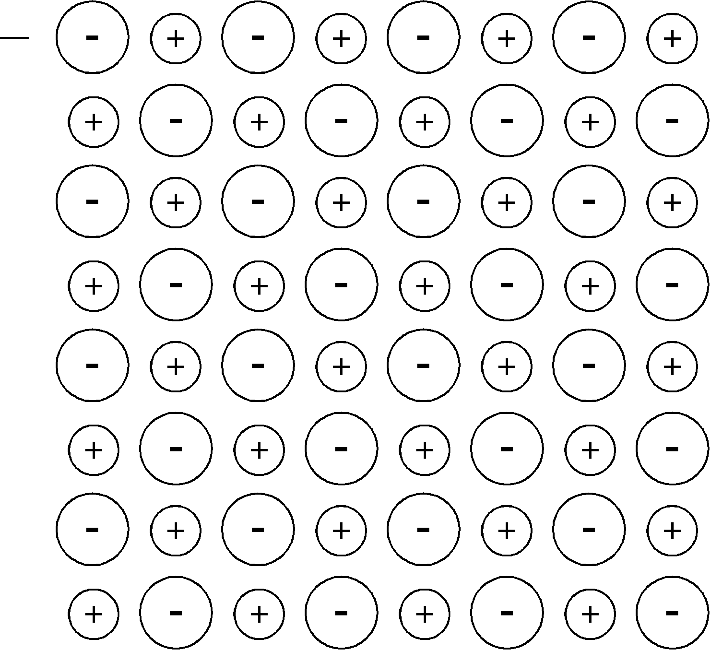
\includegraphics[width=0.4\textwidth]{type_1_tasker} & (b)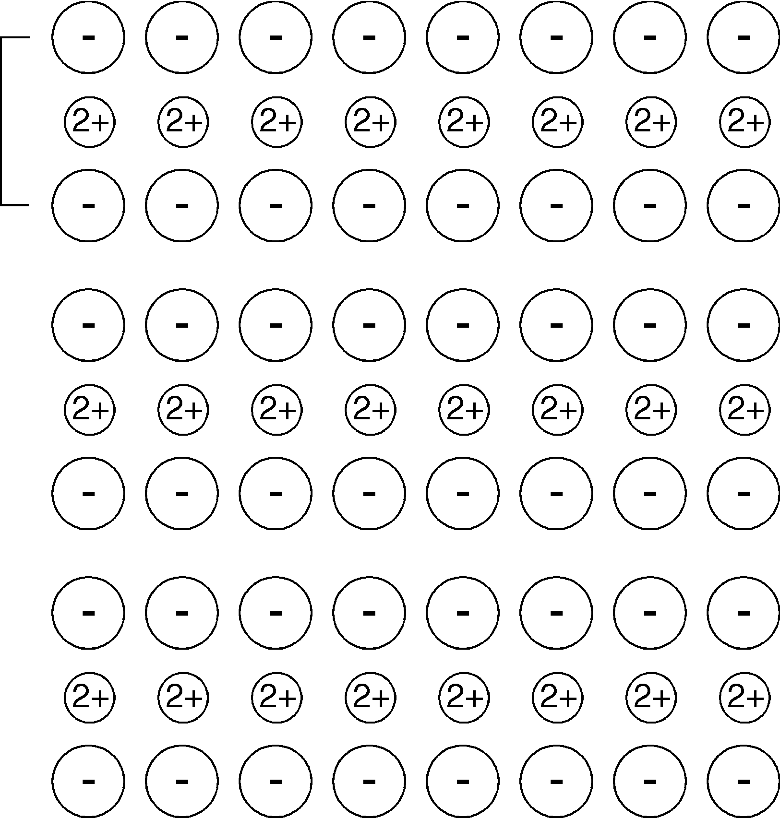
\includegraphics[width=0.4\textwidth]{type_2a_tasker}\tabularnewline
 & \tabularnewline
(c)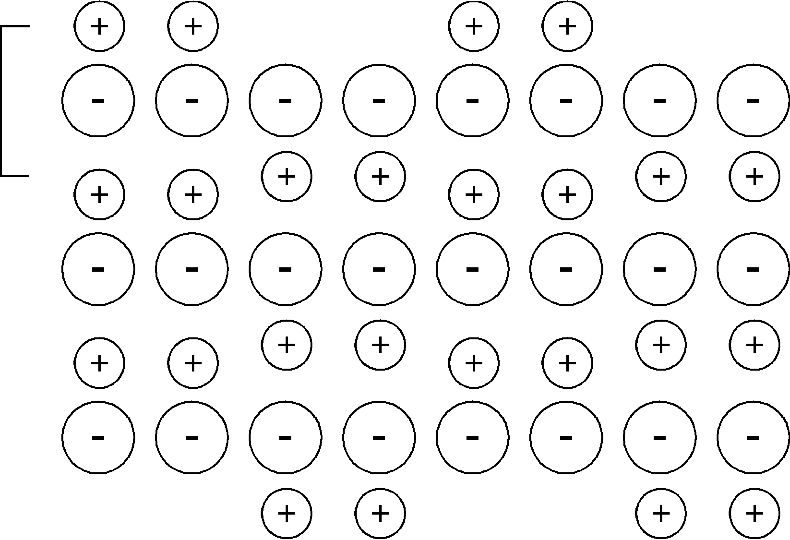
\includegraphics[width=0.4\textwidth]{type_2b_tasker} & (d)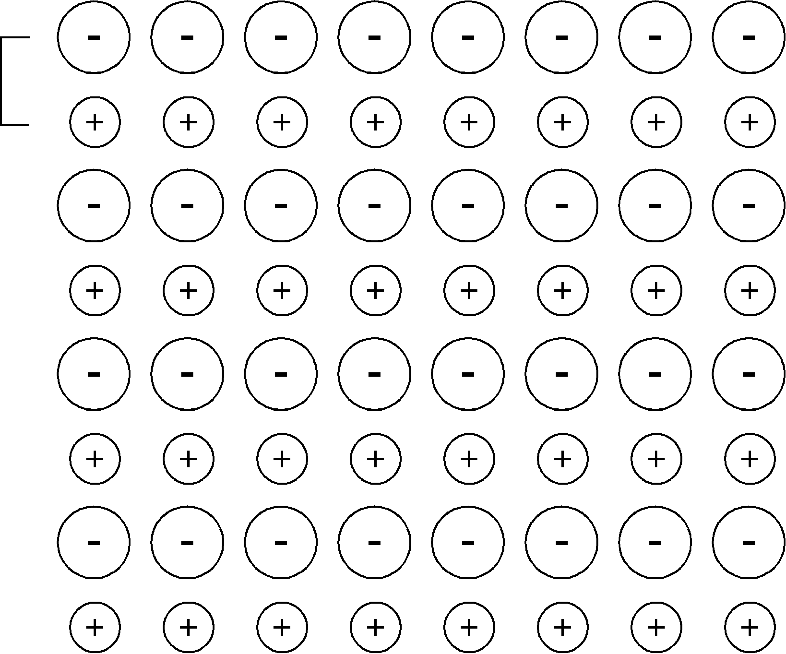
\includegraphics[width=0.4\textwidth]{type_3_tasker}\tabularnewline
\end{tabular}
\end{figure}


%
\begin{figure*}
\caption{\label{Surface types}The examples of the three types of surface illustrated
using polymorphs of calcium carbonate; (a) type I (b) type II and
(c) type III. The type I and III surfaces illustrated are from the
crystal structure of calcite, which due to its high symmetry has no
type II surfaces present. The type II example is from aragonite.}


\medskip{}


\begin{centering}
\subfigure[Type I]{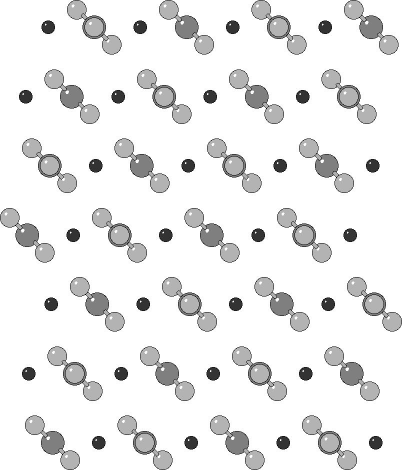
\includegraphics[height=0.35\textwidth]{type_1}}
\subfigure[Type II]{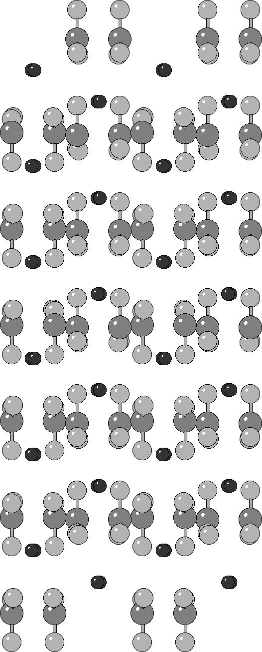
\includegraphics[height=0.35\textwidth]{type_2}}\subfigure[Type III]{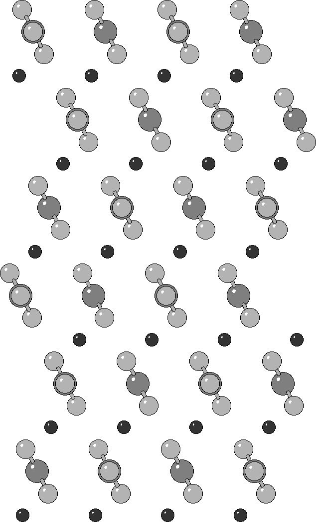
\includegraphics[height=0.35\textwidth]{type_3}}
\par\end{centering}
\end{figure*}


From the above, it can be seen that often the creation of the surface
is a significant task in its own right and can be a complex process.
In previous programs for surface calculations, the structure manipulation
has usually been performed via the input deck of the code. Clearly,
when reconstructions are involved this can become rather unwieldy.
As a result, a different strategy has been adopted for use with GULP.
All construction of the surface and structural manipulation is performed
independently from the main forcefield engine by graphical means.
This is achieved through an interface to the freely available program
GDIS developed by Dr Sean Fleming (http://gdis.seul.org/). This interface
allows surfaces to be specified by their Miller indices, valid shifts
to be searched for, and the geometries then to be manipulated, if
necessary. Once the desired surface structure has been generated,
then the necessary GULP calculation can be performed.


\subsubsection{Surface energy}

The thermodynamic penalty for cleaving a surface from a bulk material
is measured according to the surface energy. Given a bulk energy of
$U_{bulk}$ and an energy for the same system with a surface created
of $U_{surface}$, then the surface energy, $\Delta U_{SE}$, is defined
as an intensive quantity according to:\[
\Delta U_{SE}=\frac{\left(U_{surface}-U_{bulk}\right)}{A}\]
where $A$ is the resulting surface area. By definition, for any stable
material the surface energy will be endothermic. A calculated negative
surface energy implies that a material should dissociate, i.e. the
crystal should disperse into the surrounding medium.

There are two practical approaches that are widely used to determine
the surface energy by computational means. In the first, a two-dimensional
slab of material is created from the bulk, thus creating two surfaces
overall. This method has the advantage that it can be used within
programs that only allow for three-dimensional boundary conditions
through the introduction of a sufficently large vacuum gap between
the images, such that the surfaces don't interact across the vacuum.
In addition, it becomes necessary to assess whether the slab is also
thick enough since the properties must converge to those of the bulk
at the centre of the slab. In the second method, a single surface
is created by employing a two region strategy, as shown in Figure
\ref{Surface regions}. Here the solid is divided into region 1, which
contains the surface and all layers of atoms below it that exhibit
a significant atomic relaxation, and region 2, which contains the
rest of the bulk material where it is assumed that no displacements
from the three-dimensional crystal structure are induced. In practice,
only the atoms of region 2 that have an interaction with region 1
need be explicitly considered, and so the depth of region 2 is controlled
by the cut-offs of the forcefield and the Parry sum used for the electrostatics.
This second method is the most efficient and precise for atomistic
techniques. However, it is considerably harder to extend to quantum
mechanical methods since the electronic perturbations may extend further
into the bulk and embedding, typically via Green's functions, is required
to determine the influence of the electronic structure of region 2
on region 1. Through the GDIS interface, it is possible to automatically
estimate the required region 1 and 2 sizes needed to converge the
surface energy (with a default tolerance of $0.001J/m^{2}$) based
on the unrelaxed surface energies. However, if there are strong relaxations
of the surface, it may be necessary to further verify that the relaxed
surface energy is sufficiently converged.

%
\begin{figure}
\caption{\label{Surface regions}The two region surface simulation cell viewed
at right angles to the surface normal, where solid vertical lines
denote the boundaries between two-dimensional periodic images of the
cell and the dash line indicates the boundary between region 1 and
the frozen region 2.}


\begin{centering}
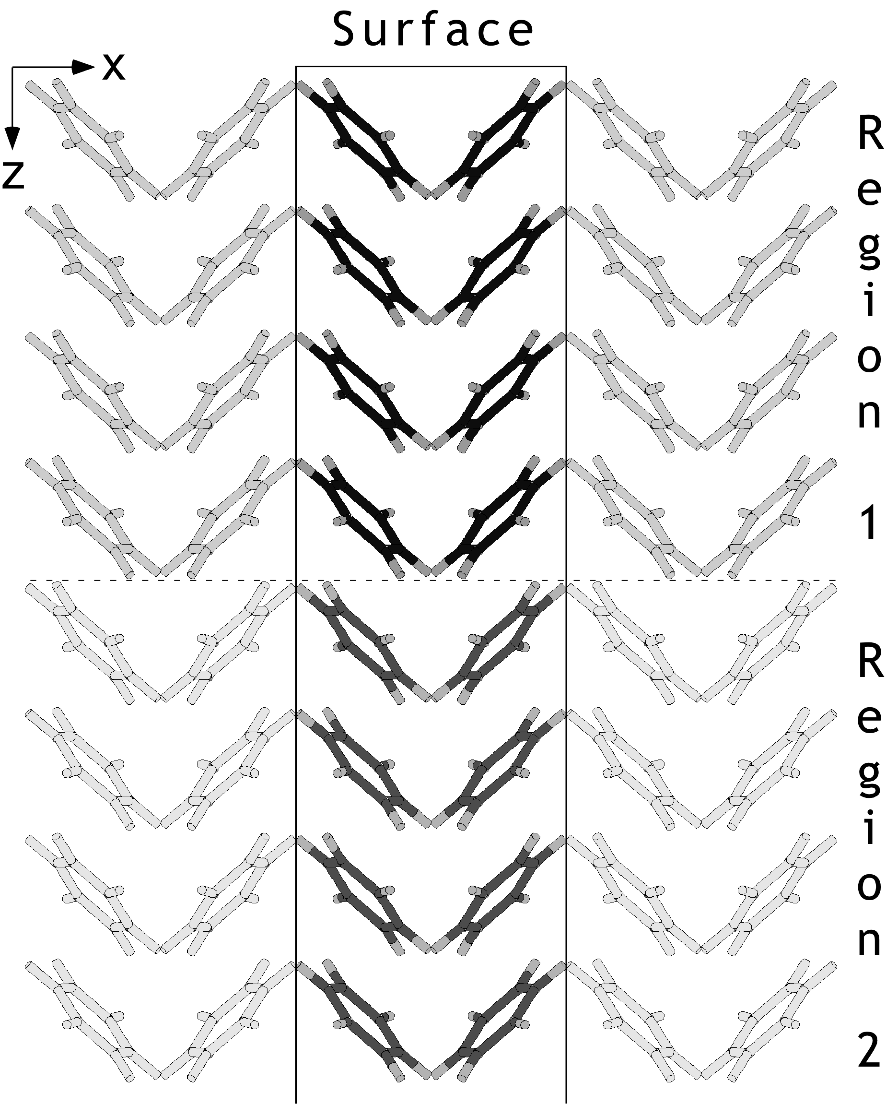
\includegraphics[width=0.8\textwidth]{cell}
\par\end{centering}
\end{figure}


The total energy for a surface calculation comprising two regions
can be written in terms of the interaction energies within, and between,
the different regions:\[
U_{tot}=U_{11}+U_{12}+U_{22}\]
The energy of region 2 with itself, $U_{22}$, is not particularly
meaningful, since the region 2 is just a partial representation of
the effectively infinite bulk material below, and any given particle
within this region will not experience the full set of interactions
that it should. However, this term is just an additive constant that
is unaltered on energy minimisation, or any other displacement of
region 1. Consequently it can be ignored in calculations. In the two
region model, the energy required to determine the surface energy
is given by:\[
U_{surface}=U_{11}+\frac{1}{2}U_{12}\]
Note that while the above energy only includes half of the region
1-region 2 interaction energy, the objective quantity for energy minimisation
is the total energy, which includes the full value of $U_{12}$. This
is because the energy change of region 2 must be allowed for when
optimising. 


\subsubsection{Attachment energy}

The surface energy, described above, provides a measure of the thermodynamic
stability of a cleavage plane. However, there is a widely used alternative
criterion which is the attachment energy. This is the energy associated
with the addition of a stoichiometric layer of material on to the
surface cut:\[
U_{attachment}=U_{tot}^{n+1}-U_{tot}^{n}-U_{tot}^{1}\]
where $U_{tot}^{n}$ represents the total internal energy of a surface
model consisting of $n$ growth layers, and $U_{tot}^{1}$ is the
energy of the growth layer alone. For any stable material, this implies
that the attachment energy must be an exothermic quantity. In practice,
the calculation of the attachment energy is obtained from the energy
of interaction of the growth layer at the surface with the rest of
the underlying material. This benefits from the fact that the attachment
energy can be obtained from a single calculation, just as is the case
for the surface energy, rather than by performing the actual addition
of a layer as part of a multistage process. 

Although the attachment energy is also a strictly thermodynamic quantity,
it is often regarded as representing the kinetics of crystal growth
because of the conceptual link between the ease of the addition of
a growth layer and the rate at which a surface is added to. Consequently,
those faces where the attachment energy is most exothermic will tend
to grow most rapidly.


\subsubsection{Morphology}

The morphology of a crystal is the macroscopic shape that it adopts.
Because this can be readily observed for nearly all materials, either
under an electron microscope or, in the case of many naturally occuring
minerals, by visual inspection with the naked eye, it should provide
a ready means to test the validity of a simulation model. Of course,
the reality is rather more complex, since the morphology is sensitive
to the presence of impurities, the nature of the solvent used as the
growth medium, and many other factors relating to the sample preparation.
Consequently there are materials where many different morphologies
can be observed for the same compound. A classic example, is that
of calcite ($CaCO_{3}$), where there are both several different polymorphs
of the bulk material and several hundred different known morphologies.
Many of these variations result from biomineralisation by different
species. Despite this, for many pure inorganic materials morphological
prediction using atomistic techniques is surprisingly successful.

Crystal morphologies can be calculated based on either the surface
energy or attachment energy, which are typically taken to represent
growth under conditions of thermodynamic and kinetic control, respectively.
In order to do this, it is first necessary to determine the objective
quantity for all significant faces. Given that dipolar faces are usually
unstable, the number of likely cleavage planes for most materials
is actually considerably smaller than initially might be conceived
of based on permutations of the Miller indices. Furthermore, where
there is space group symmetry present for the bulk, many surface planes
are equivalent, thus reducing the number of unique faces. Finally,
only those faces with the largest interplanar spacings are likely
to appear in the morphology \cite{DonnayHarker}. The actual morphology
is generated as a three-dimensional Wulff plot \cite{key-119}. Here
the ratio of the surface normal distances of all planes from the centre
of the polyhedron are determined according to the either the surface
or attachment energy. The final shape of the polyhedron is then determined
by the intersection of the cleavage planes. Unstable surfaces lie
outside the polyhedron and never intersect. Morphological plots can
also be produced through the GDIS interface to GULP.

In the equilibrium morphology approach, the contribution of a given
plane to the total surface area is inversely proportional to its surface
energy \cite{GibbsMorph}. For the growth morphology methodology \cite{HartmanMorph},
the surface area contribution is again inversely proportional, but
now to the negative of the attachment energy. This is because surfaces
with a highly exothermic attachment energy will rapidly grow out of
the morphology to leave the slow growing bounding faces.


\subsubsection{Surface phonons}

The calculation of the phonons of a 2-D slab is exactly analogous
to that for the three dimensional case, except that the Brillouin
zone is also now two dimensional leading to dispersion only in the
$xy$-plane (taking $z$ to be the direction of the surface normal). 

Turning to consider the standard two region surface model, there are
some important issues to consider. Because region 2 is quasi-infinite,
it is only possible to determine the phonons for the particles in
region 1. Therefore, the dynamical matrix is constructed based on
region 1 alone, but with contributions to the on-diagonal matrix blocks
from the potential experienced due to a rigid, non-vibrating region
2. Consequently it is assumed that the vibrations of the two regions
are completely decoupled. Since this is an approximation, the frequencies
near the interface of the regions will be slightly in error, particularly
in the low frequency regime where coupling is generally strongest.
However, the surface modes, which are usually the ones of primary
interest, will be less affected. As always, it is essential to monitor
the convergence of all quantities with respect to increasing the region
1 depth. Finally, because region 1 is vibrating under the influence
of an external potential, the first three frequencies at the $\Gamma$-point
will no longer be zero, though they typically will be small.

\subsection{Continuum solvation of surfaces}

In the above description of surface properties the surface is always assumed
to be in contact with vacuum. However, the properties of surfaces in contact
with solvent are equally as important. While the interface between a solid and
liquid is most accurately studied using molecular dynamics simulations, there
are some situations where more approximate methods are valuable. For
example, to predict the solvent dependent morphology of a crystal only requires
the ratio of the surface energies to be correct and not the absolute magnitude. 
To perform molecular dynamics to extract the relative free energies of solvation
for a large collection of surface is very challenging and time consuming. Here
the use of a more approximate approach is valuable. 

In GULP the option to employ a continuum solvation model has been added.
Here the solvent accessible surface is described using a grid of points and the
response of the solvent due to its dielectric properties calculated at this surface
in response to the electrostatic potential of the solid. Full details of the method
implemented in GULP can be found in the literature \cite{COSMIC}. In brief, 
the method uses the COnductor-like Screening MOdel (COSMO) of Klamt
and Schuurmann \cite{COSMO}, but with a few modifications. The solvent accessible surface
(SAS) is smoothed by use of tapering functions, and octahedral triangulation is
used to generate the points in order to maximise symmetry. Furthermore, the
frame of a molecule (if applied in 0-D) is rotated according to the eigenvectors
of the moment of inertia tensor in order to ensure rotational invariance. The
final change is more significant; because the induced charge on the solvent
accessible surface is unconstrained the total charge of a surface and solvent
could be non-zero (and non-integer). When working within periodic boundary
conditions it is essential to maintain charge-neutrality such that a convergent
electrostatic energy can be obtained. To do this GULP uses the COSMO method
under the constrain of Integer Charge (COSMIC) to ensure that the electrostatics
remain valid. 

The current implement of the COSMIC continuum solvation model can be 
applied to surfaces, polymers, solids and molecules. Both analytic first and
second derivatives are available, though phonons can only be evaluated at
the gamma point at present. 

\subsection{Free energy minimisation}

One of the most important issues in solid state modelling is the variation
of materials properties with the applied conditions. While isotropic
external pressure is trivial to incorporate, as has already been shown,
inclusion of the effect of temperature is more complex. This process
is exacerbated by the fact that the majority of potentials have been
derived through the use of some empirical (i.e. experimental) data
which has been measured under a given set of conditions. Hence the
forcefield itself can often already contain an implicit temperature,
or worse, if multiple pieces of experimental data have been employed
that were measured at different conditions, it can be a convolution
of several temperatures. One solution to this is to extract forcefields
from quantum mechanical methods so that everything is obtained explicitly
at absolute zero. For now, we will assume that the forcefield has
been derived so as to be free of implicit temperature effects, by
whatever means.

There are several distinct approaches to the inclusion of temperature
into simulations. Which one is most appropriate depends on the particular
temperature and nature of the system. In the low temperature regime,
the atoms of the crystal structure just execute vibrations about their
lattice sites, which in the limit of absolute zero will be purely
harmonic. This situation is best described through the use of lattice
dynamics, which is the quasi-static approach to treating a vibrating
lattice. As the temperature increases, the motions will become increasingly
anharmonic. In principle, this can be handled, to a point, through
the use of anharmonic corrections to the harmonic lattice dynamics,
in order to allow for weak phonon-phonon coupling. However, when the
temperature becomes sufficiently high that diffusion can occur it
is necessary to switch to an alternative approach. Typically one of
two approaches can then be employed. If detailed information is required
concerning the atomic motions and related properties, then the method
of choice is molecular dynamics \cite{MDGeneralRef}. This propagates
Newton's equations of motion through time using a finite difference
formalism. Hence it retains time correlation functions and the trajectories
of all atoms. Its strength is that anharmonic effects are fully included.
However, since it regards nuclei as classical particles, it is invalid
at low temperatures due to the neglect of the quantisation of vibration
and zero point motion, unless the Path-Integral formalism is employed.
It can be seen therefore that lattice dynamics and molecular dynamics
are largely complementary in their regions of applicability. Although
GULP also includes the capability to perform molecular dynamics, this
topic will not be discussed here since this area, in regard to other
codes, has been discussed elsewhere \cite{DLPOLY2}, and the more
unique, static, features will be focussed on here. Likewise, the effect
of temperature can also be explored through Monte Carlo simulation
\cite{MonteCarloGeneralRef}, if the focus is integration over phase
space, with no regard to timescale or kinetic factors, but this topic
will not be discussed further because it is not one of the more novel
features of GULP.

Concentrating now on the use of lattice dynamics for examining the
temperature dependance of crystal properties, the dominant effect
is the change in the crystal structure. When heated, most materials
undergo thermal expansion which correspondingly leads to softening
of many of the mechanical properties. There are a few celebrated examples
of materials that actually contract on heating, through the rotation
of quasi-rigid polyhedra, which is technologically very important
in the quest for zero thermal expansion composites.

It has already been shown that it is possible to calculate the Helmholtz
free energy for a given structure as a function of temperature through
the determination of the vibrational partition function from the phonon
density of states. Hence, a natural approach to determine the dependance
of structure on temperature is through free energy minimisation. Here
the key foundation is the quasi-harmonic approximation, which assumes
that the vibrational frequencies can be determined as if the atoms
are vibrating purely harmonically while the cell parameters are adjusted
to minimise the free energy. Previous studies have indicated that
this is a reasonable approximation until a temperature of approximately
half the melting point has been reached.

The major barrier to free energy minimisation is that we have already
seen that efficient optimisation requires at least the first derivatives
of the quantity with respect to the structural variables. Hence a
number of approaches evolved for tackling this problem. LeSar \textit{et
al} \cite{key-90} developed a method whereby the atoms where represented
as Gaussian distributions, whose width represented the vibrational
motion. The Gaussian exponent was then regarded as a variational parameter
that minimised the free energy. Hence the free energy could be obtained
without direct recourse to a phonon density of states, making derivatives
straight forward. While this approach is easy to apply to metals,
the extension to a more complex ionic systems is more demanding. A
method that approximated the phonon density of states was introduced
by Sutton \cite{key-88}, which involved taking moments of the dynamical
matrix, as pioneered by Montroll \cite{key-89} several decades earlier,
and in the spirit of tight binding theory. This approach has the advantage
that the derivatives are taken of the dynamical matrix elements, rather
than of phonon frequencies, which are the product of a matrix diagonalisation.

In the field of ionic materials, Parker and Price \cite{key-91} pioneered
the use of free energy minimisation through the use of numerical derivatives.
Here central finite differences were taken with respect to the cell
strains, with the internal degrees of freedom being formally optimised
at every point. This approach had the advantage over the other methods
that no approximation was being introduced beyond the quasiharmonic
one. However, because this requires $\left(2N+1\right)$ optimisations
and phonon evaluations per energy/gradient evaluation with respect
to the free energy, the minimisation was restricted to the strains
alone in order to reduce the number of variables, $N$, to a maximum
of six.

More recently, Kantorovich \cite{key-92} has derived expressions
for the analytical derivatives of the free energy, which were implemented
contemporaneously in the program SHELL of Allan and co-workers \cite{key-93},
and in GULP \cite{key-94}. If we consider the differential with respect
to strain, though the expressions would be identical for any degree
of freedom, then the first derivative of the free energy is given
by:\[
\left(\frac{\partial A}{\partial\epsilon}\right)=\left(\frac{\partial U_{static}}{\partial\epsilon}\right)+\sum_{k}\sum_{m}\left\{ \frac{h}{2\omega}\left(\frac{1}{2}+\frac{1}{\exp\left(\frac{h\omega}{k_{B}T}\right)-1}\right)\left(\frac{\partial\omega^{2}}{\partial\epsilon}\right)\right\} \]
where the expression is written in terms of the derivatives of the
square of the frequencies, since these values represent the eigenvalues
of the dynamical matrix. Their derivatives can be calculated through
the application of perturbation theory and expressed as the derivatives
of the dynamical matrix projected onto the corresponding eigenvectors:\[
\left(\frac{\partial\omega\left(k,m\right)^{2}}{\partial\epsilon}\right)=e_{m}^{*}\left(k\right)\left(\frac{\partial D\left(k\right)}{\partial\epsilon}\right)e_{m}\left(k\right)\]
In order to determine the derivatives of the phonon frequencies, we
therefore require the phased third derivatives of the energy with
respect to either three Cartesian coordinates, or two Cartesian coordinates
and one strain. for internal and external variables, respectively.

For the most efficient optimisers, based on Newton-Raphson techniques,
we strictly need the second derivatives with respect to the free energy,
which corresponds to the fourth derivatives of the internal energy.
However, this is considerably more expensive and complex, so the Hessian
matrix is usually approximated by the conventional internal energy
Hessian by assuming that the free energy contribution to the curvature
is small. Furthermore, the use of updating formulae will ultimately
correct for the discrepancy given sufficient optimisation steps.

With the advent of analytical derivatives, it is now possible to consider
two types of free energy minimisation. The first has been christened
the Zero Static Internal Stress Approximation (ZSISA) by Allan and
co-workers \cite{key-129}, which resembles the approach taken with
numerical first derivatives (i.e. the unit cell is minimised with
respect to the free energy, while maintaining the internal degrees
of freedom at a minimum with respect to the internal energy). When
working within this formalism there is an additional contribution
to the strain derivatives, which corrects for the fact that internal
degrees of freedom are not at a minimum with respect to the free energy:\[
\left(\frac{\partial A}{\partial\epsilon}\right)_{ZSISA}=\left(\frac{\partial A}{\partial\epsilon}\right)-\left(\frac{\partial^{2}A}{\partial\epsilon\partial\alpha}\right)\left(\frac{\partial^{2}A}{\partial\alpha\partial\beta}\right)^{-1}\left(\frac{\partial A}{\partial\beta}\right)\]
Here the approximation is again made that the second derivative matrices
can be approximated by neglecting the free energy contribution; an
approximation that should be enhanced by the cancelation that results
from taking a ratio. The second type of optimisation can be called
full free energy minimisation (FFEM), in which the internal degrees
of freedom are also minimised with respect to the free energy. This
is potentially appealing since sometimes it is the details of the
internal changes that might be of interest, for example, the nature
of an adsorption complex within a microporous material. 

Results for silicate materials show a number of interesting features
regarding the merits of both approaches. Firstly, in the case of $\alpha$-quartz
where accurate experimental data is available for comparison, it appears
that the ZSISA approach underestimates the thermal expansion, while
the FFEM method is more accurate, though of course this is subject
to the limitations of the specific potential model chosen \cite{key-94}.
However, for all silicates tried so far the full minimisation approach
goes catasrophically wrong at about ambient conditions. This is illustrative
of a general problem with this approach which tends to drive systems
to instability. This can be readily understood, since the free energy
is minimised by creating phonons that tend to zero frequency and hence
the structure is motivated to create soft modes. This behaviour does
not tend to happen in the ZSISA approach where only the cell strains
are directly coupled to the free energy and thus the relaxations tend
to lead only to a scaling of modes, rather than more individual changes.
Hence the use of ZSISA is far more robust and generally recommended
for most purposes.


\subsection{Monte Carlo}

An alternative approach to including temperature into results, if
one is not interested in the time correlation properties, just the
ensemble averages, is Monte Carlo simulation. Here the distribution
of positions according to a Boltzmann distribution is determined numerically
for a specified temperature and conditions. Under the Metropolis importance
sampling scheme, if a randomly chosen move for the system leads to
a lowering in the energy then the move is accepted and the system
evolves to the new state. If the energy increases, then the move is
accepted with a probability given by:\[
P=\exp\left(-\frac{\Delta U}{k_{B}T}\right)\]
where $\Delta U$ is the energy change associated with the move. There
are several types of move available for a system as listed below:

\begin{itemize}
\item Translation - this allows atoms or molecules to move in x, y or z,
according to the flags set
\item Rotation - for rigid molecules, this allows the molecule to sample
the rotational distribution
\item Creation/destruction - in the Grand Canonical ensemble, molecules
can be inserted or removed to a reservoir of molecules whose chemical
potential is specified
\end{itemize}
Note that the Monte Carlo feature is relatively new and should be
considered as a beta release available to those who wish to test. 


\subsection{Defect calculations}

While the simulation of bulk material properties is important, just
as crucial is the study of both intrinsic and extrinsic defects. Many
of the key applications of solid state systems, such as catalysis,
electronic and ionic conductivity, ion exchange and waste immobilisation,
critically depend on the utlisation of the characteristics of defect
centres. Consequently, from the early days of the field of atomistic
simulation defect studied have been one of the most vigorously pursued
topics.

There are two widely used approaches for performing defect calculations
on solids; the supercell and the cluster methods, with or without
embedding in the latter case. Both approaches have their merits and
demerits. Putting computational implementation factors aside, the
use of embedded clusters is ideal for the infinitely dilute limit,
while the supercell method is more appropriate for high concentrations
of defects where there exists significant defect-defect interaction.
In practice, the nature of the computational method often biases the
method of choice. However, with atomistic techniques both approaches
are feasible. Since the supercell method is simply the extension of
a bulk calculation, we will focus here on the embedded cluster approach.
In this particular context, the technique is generally referred to
as the Mott-Littleton method \cite{key-95}, after the authors of
the pioneering work in the field, though the implementational details
differ a little from their original work.

The basis of the Mott-Littleton method is the so-called two region
strategy. Here a point called the defect centre is defined, which
typically lies at a point concentric with the initial defect site,
or, where there is more than one defect, at the mid-point of the ensemble
of point defects. The crystal around the defect centre is divided
into two spherical regions, with the inner sphere being labelled region
1, and the outer spherical shell of ions being region 2a. Atoms outside
of these spheres belong to region 2b, which then extends to infinity.
The dimensions of these regions are typically specified either by
their radii or the number of ions contained within them. The ions
in region 1 are assumed to be strongly perturbed by the defect and
therefore are relaxed explicitly with respect to their Cartesian coordinates.
In contrast, the ions in region 2 are assumed to be weakly perturbed
and therefore their displacements, with the associated energy of relaxation,
can be approximated in some way. Clearly, as the region 1 radius is
increased these approximations will become increasingly valid, and
thus an important stage of a defect calculation is to ensure that
the defect energy is sufficiently converged with respect to the region
radii. In some cases the convergence of the absolute defect energy
can be slow, in which case it may be sufficent to monitor the convergence
of relative defect energies instead. As a guideline, the radius of
region 1 and the difference of the radii of regions 1 and 2 should
be both be greater than the short-range potential cut-off to achieve
convergence, though for charged defects this may not be adequate.

Within the Mott-Littleton scheme, we can express the total energy
of the two region system as the sum of contributions from the energies
within the regions and between them:\[
U_{tot}\left(x,\xi\right)=U_{11}\left(x\right)+U_{12}\left(x,\xi\right)+U_{22}\left(\xi\right)\]
where $U_{11}\left(x\right)$ represents the energy of region 1 as
a function of the Cartesian coordinates, $x$, $U_{22}\left(\xi\right)$
represents the energy of region 2 as a function of the Cartesian displacements,
$\xi$, and $U_{12}\left(x,\xi\right)$ is the energy of interaction
between the two regions. At this stage we do not distinguish between
regions 2a and 2b. If the forces acting on region 2 are small, then
we can assume that the response of the atoms in this region will be
purely harmonic. Hence, the energy of region 2 can be written as:\[
U_{22}\left(\xi\right)=\frac{1}{2}\xi^{T}H_{22}\xi\]
where $H_{22}$ is the Hessian matrix for region 2. If we now apply
the condition that the displacements in region 2 will be the equilibrium
values this yields the following condition:\[
\left(\frac{\partial U_{tot}\left(x,\xi\right)}{\partial\xi}\right)_{x}=\left(\frac{\partial U_{12}\left(x,\xi\right)}{\partial\xi}\right)_{x}+H_{22}\xi=0\]
Combining this equation, and the previous one, it is possible to eliminate
the energy of region 2 from the total energy without direct recourse
to the Hessian matrix (which would be of infinite dimension):\[
U_{tot}\left(x,\xi\right)=U_{11}\left(x\right)+U_{12}\left(x,\xi\right)-\frac{1}{2}\left(\frac{\partial U_{12}\left(x,\xi\right)}{\partial\xi}\right)_{x}\xi\]
Thus the problem of calculating the energy of region 1 in the potential
of region 2 has been reduced to evaluating the energy of region 1
and its interaction with region 2, without having to evaluate the
self energy of region 2. Furthermore, in order to lead to partial
cancellation of terms, the quantity calculated is the defect energy
- i.e. the difference between the energy of the perfect region 1 and
2, $U_{tot}^{p}$, and the defective case, $U_{tot}^{d}$, rather
than the individual contributions:\[
U_{defect}\left(x,\xi\right)=U_{tot}^{d}\left(x,\xi\right)-U_{tot}^{p}\left(x,\xi\right)\]
It should be noted that it is assumed that the energy of any species
removed or added during the formation of the defect has an energy
of zero at infinite separation. If this is not the case, then the
defect energy must be corrected \textit{a posteriori} for this. However,
such corrections have no influence on the outcome of the defect calculation
itself.

There is one important consequence of the above formulation of the
total defect energy, in that it becomes necessary to find the optimised
energy with respect to the Cartesian coordinates of region 1 by force
balance, rather than by energy minimisation. The point at which the
forces tend to zero is usually only slightly different from the minimum
in the internal energy, depending on the degree of perturbation of
region 2. Hence, during an optimisation of the defect energy GULP
initially minimises the energy, as per a conventional Newton-Raphson
procedure. Once the gradient norm falls below a specified tolerance,
and region 1 lies within the harmonic region, then the harmonic displacements
according to the Hessian and gradients are applied without the use
of a line search until the forces drop below the specified tolerance.

A further important point relates to the state of the bulk crystal
when performing defect calculations. Because of the use of displacements
in region 2, it is crucial that the bulk structure is at an energy
minimium with respect to the internal coordinates before performing
a defect calculation. Hence the bulk crystal must be relaxed to equilibrium
at least at constant volume, if not at constant pressure. Furthermore,
it is also important that there are no imaginary phonon modes within
the Brillouin zone otherwise the displacements in region 2 may correspond
to unstable harmonic equilibrium. The presence of such modes is the
most common cause of unphysical results, for instance obtaining negative
defect energies for intrinsic defects. Because the presence of defects
lowers the symmetry, a Mott-Littleton calculation may encounter instabilities
not apparent for the bulk material.

Now it is necessary to consider the treatment of region 2 in more
detail, and in particular the difference between regions 2a and 2b.
In region 2a, the forces on the individual ions due to short-range
interatomic potentials and the Coulomb term are explicitly calculated
and the local displacement evaluated. While the forces on region 2a
are technically due to all ions in region 1, a commonly used approximation
is to evaluate the forces due to defect species only. This is the
approach taken in the default calculation method for compatability
with earlier results.

In contrast to the above situation for region 2a, for region 2b the
energy of relaxation must be determined implicitly since this region
extends to infinity. It is assumed that in region 2b the only force
acting is that due to the Coulomb potential in order to simplify the
problem. By choosing the radius of region 2a to always be greater
than that of region 1 by the short-range potential cut-off this can
always be arranged to be valid. Even having retained only the Coulomb
interaction in the perturbation of region 2b, this still leaves many
interactions to consider. To simplify the problem, the electrostatic
potential due to defects in region 1 can be represented by the multipole
moments of the deformation situated at the defect centre. If region
2a is sufficiently large, then the only significant term will be the
monopole moment of the defect (i.e. the net charge). Hence, the energy
of region 2b is evaluated as the induced relaxation energy due to
the net charge of the defect situated at the specified defect centre.
While this is a significant approximation, it usually works well in
practice and again becomes valid with increasing region sizes. In
the original Mott-Littleton method, the interaction with region 2b
was described by a continuum approximation. However, in subsequent
implementations a sum of the induced polarisation energy is performed
over the atomic sites. For the general case of an anisotropic dielectric
constant tensor \cite{CatlowJamesStewartMackrodt}, the energy of
region 2b is calculated as:\[
U_{2b}=-\frac{1}{2}Q^{2}\left(\sum_{i\in2b}\sum_{\alpha\beta}\frac{M_{i}^{\alpha\beta}r_{ci}^{\alpha}r_{ci}^{\beta}}{r_{ci}^{6}}\right)\]
where $Q$ is the net charge of the defect, $r_{ci}$ is the distance
of the $i$th atom from the defect centre, and $M_{i}^{\alpha\beta}$
is a 3 x 3 matrix for each atomic site, in the Cartesian frame, that
represents the on-site polarisability. The quantitative definition
of the matrix elements $M_{i}^{\alpha\beta}$ is \cite{hades}:\[
M_{i}^{\alpha\beta}=\sum_{\gamma}\left(\left(D^{-1}\right)^{\alpha\gamma}q\right)_{i}\left(\epsilon^{-1}\right)^{\gamma\beta}\]
where $D_{i}^{-1}$ represents the on-diagonal block of a modified
inverse second derivative matrix and $\epsilon$ is the static dielectric
constant tensor. Note that the inverse of the second derivative matrix
is singular and therefore a further approximation must be made. Physically,
this problem corresponds to the division of the polarisation between
the sublattices being arbitrary. The usual solution taken is to assume
that the polarisation is divided equally between the cation and anion
sublattices, with the second derivative matrix being modified correspondingly.
In the special case of a cubic crystal, the expression for the region
2b energy can be simplified to:\[
U_{2b}=-\frac{1}{2}Q^{2}\left(\sum_{i\in2b}\frac{m_{i}}{r_{ci}^{4}}\right)\]
where $m_{i}$ is the average of the diagonal elements of the matrix
$M$ (for the cubic case these will all be equal, but if the isotropic
formula were to be applied in a non-cubic case this would not be so).

Because the expression for the region 2b energy is not particularly
short-ranged, it is appropriate to evaluate it using lattice summation
techniques analogous to those applied to the monopole-monopole term.
Hence the term is summed to convergence based on a perfect infinite
lattice and then the contributions from ions in regions 1 and 2a are
subtracted off. The distance dependent factor within the expression
for the energy can be rewritten as:\[
\frac{r^{\alpha}r^{\beta}}{r^{6}}=\frac{1}{8}\left(\frac{\partial^{2}\left(\frac{1}{r^{4}}\right)}{\partial r^{\alpha}\partial r^{\beta}}\right)+\frac{\delta_{\alpha\beta}}{4}\left(\frac{1}{r^{4}}\right)\]
Hence, by evaluating the equivalent of the Ewald summation for the
inverse fourth power of distance, and its second derivatives with
respect to Cartesian displacements, it is possible to achieve a rapidly
convergent expression for the energy of region 2b.

Having described how defect energies are calculated in theory, we
mention a few practical points. There are three types of defect that
can be specified within GULP:

\begin{itemize}
\item Vacancy
\item Interstitial
\item Impurity
\end{itemize}
The last one of these three is clearly the combination of a vacancy
and an interstitial at the same atomic position in the structure.
The location of a vacancy or an impurity can be specified by reference
to either a spatial position or an atom position by referencing the
site. An interstitial, by its very nature, must be specified by coordinates.
When an atom is designated to be vacant, then both the core and shell
will be removed automatically since it would not be sensible to leave
one or the other present in the system. It is also possible to specify
that a whole molecule be removed from the system, when the connectivity
has been defined.

Most types of calculation, that are logically applicable, can also
be applied to defect runs, such as optimisation to a minimum or a
transition state. In the case of vibrations, the frequencies are calculated
for a dynamical matrix based on region 1. In must be noted that this
is a large approximation, since any modes that are coupled between
regions 1 and 2 will not be properly described. Only localised modes
relating to atoms near the centre of region 1 will be correctly predicted.
Consequently such calculations of vibrations must be interpreted cautiously.

Finally, a degree of point group symmetry may be utilised during defect
calculations. An automatic search for common symmetry elements is
performed about the defect centre, including mirror planes and $C_{2}$
axes that are aligned with, or between, the Cartesian axes. Such symmetry
is used to reduce the number of region 1 and region 2 atoms stored,
thereby reducing the number of degrees of freedom for optimisation,
as well as taking advantage of symmetry adapted algorithms to accelerate
the calculation of the energy and its derivatives.


\subsection{Derivation of interatomic potentials}

One of the major challenges facing anyone wishing to use forcefield
methods is to determine the functional form and parameters required
to calculate the energy and properties. In the field of organic chemistry
and biomolecules, there are a number of well-established forcefields,
such as MM3 \cite{MM2}, and those associated with the programs AMBER
\cite{amber}, and CHARMM \cite{CHARMM}, which are, in principle,
capable of handling most elements typically found in these systems
(C, H, O, N, S, P, etc) in their common hybridisation states. These
are constructed around the molecular mechanics approach where the
forcefield is connectivity driven and interactions are described in
terms of two-, three-, and four-body bonding terms, plus long-range
Coulomb and non-bonded interactions. While there have been several
attempts to generate general forcefields that cover the entire periodic
table, such as UFF \cite{UFF}, ESFF \cite{ESFF}, etc, none have
been completely successful. Because of the enormity of the amount
of data required when spanning the whole range of elements, it is
impractical to determine such a universal forcefield by empirical
fitting. Instead general rules must be used to predict parameters
based on extrapolations and intrinsic properties of the element that
are known - for instance the electronegativity. Not surprisingly,
this leads to limitations in the quality of the results. For most
inorganic systems it is usually necessary to derive a forcefield for
the specific material, or family of materials, of interest. 

There are two means by which a forcefield can generally be derived,
if we exclude rule based extrapolations. Firstly, it is possible to
obtain parameters by fitting to a potential energy surface obtained
from a non-empirical theoretical method. This would typically consist
of results from \textit{ab initio} calculations, ideally on the periodic
solid \cite{AluminaFit}, or perhaps on a gas phase cluster, or even
better, both of the aforementioned sources. The potential energy surface
can be fitted either as a sequence of geometries with their corresponding
energies, or derivatives of the energy could also be included to maximise
the amount of information from each higher level calculation. Many
of the early forcefields for ionic materials were determined using
electron gas methods \cite{ElectronGasMethods}, in which the energies
of interaction between pairs of ions were determined by a density
functional calculation using the overlapping ionic electron densities,
where the anion is confined in an appropriate potential well. Secondly,
parameters can be obtained by empirical fitting in which the normal
process of using a forcefield to determine the properties of a material
is inverted. This approach depends on the availability of a range
of experimental data. Knowledge of the crystal structure is a definite
prerequisite for this method, but is insufficient alone since information
is required as to the curvature of the energy surface about the minimum.
This later data may come from quantities such as elastic constants,
bulk moduli, piezoelectric constants, dielectric constants, or phonon
frequencies.

In order to perform a fit, first it is necessary to define a quantity
that measures the quality of the results, known as the sum of squares;\[
F=\sum_{i=1}^{N_{obs}}w_{i}\left(f_{i}^{obs}-f_{i}^{calc}\right)^{2}\]
where $N_{obs}$ is the number of observables, $f_{i}^{obs}$ and
$f_{i}^{calc}$ are the fitted and calculated values of the observable,
respectively, and $w_{i}$ is the weighting factor for the given observable.
Because of the weighting factor, there are an infinite number of possible
solutions all of which are equally valid. Hence, one of the most important
skills is knowing how to choose appropriate and sensible weighting
factors. There are several criteria that can be used for guidance
though. Firstly, if fitting experimental data, the weighting factor
should be inversely proportional to the uncertainty in the measured
value. Obviously trusted, precise values should be given more priority
than data where there are large error bars. Secondly, the weight factor
should be inversely proportional to the magnitude of the observable
squared. This ensures that all values are fitted on an equal footing,
regardless of units. For example, fitted vibrational frequencies in
wavenumbers are typically two to three orders of magnitude larger
than structural variables.

The fitting process itself involves minimising the above function
$F$. To do this, the default approach is similar to that used in
optimisation. For many terms, the evaluation of the derivatives of
the sum of squares with respect to the variables is complex, and in
some of the fitting algorithms that will be discussed subsequently
it is even impossible. As a result, numerical derivatives are employed
during fitting since it greatly simplifies the process. Because of
this, the default optimiser is to use a BFGS update of an initial
on-diagonal only Hessian, obtained by finite differences, in a Newton-Raphson
process. However, for particularly difficult cases, where correlation
between variables is strong, there is the option to use a full Hessian
matrix, again obtained by finite differences.

Now we turn to specifically consider the fitting methodology for the
case of empirical data. Traditionally, the experimental structure
is fitted by varying the potential parameters so as to minimise the
forces at this configuration, and this is the default strategy. Other
observables, such as elastic constants etc, are then calculated at
the experimental structure too. When working with the shell model,
either dipole or breathing shell, there is an additional complication
though in that while the cores are fully specified since they are
equated with the nuclei of the ions, the positions/radii of the shells
are undefined. One approach is to fit with the shells positioned to
be concentric with the cores. However, this is unphysical since it
implies that there is no ionic polarisation, which defeats the object
of including the model in the first place. A second approach might
be to place the shell according to specified ion dipoles, but this
information is almost impossible to come by. Only data about the total
polarisation of the unit cell is typically available and a unique
atomic decomposition is not possible. In order to handle this issue,
the simultaneous relaxation of shells approach was introduced into
GULP \cite{GULPFit}. Here the shells are allowed to move during fitting.
Formally, the most correct approach is to allow the shells to be energy
minimised at every evaluation of the fitting function. However, a
simpler approach has been implemented in which the shell forces are
added as observables and the shell positions become fitting variables.
In this way, the shells are minimised directly within the fitting
procedure. In the absence of any observables other than the structure,
this is exactly equivalent to minimising the shells at every step
of fitting. When observables are present there will be small differences,
but these are usually an acceptable price to pay for the greater ease
of implementation.

There is actually a more fundamental flaw with the approach of fitting
forces at the experimental geometry as a method of fitting. Often
we judge the quality of a fit by the percentage error in the structural
variables rather than the forces. Although lowering the forces during
a fit generally improves the optimised structure with respect to experiment,
this is not guaranteed to be the case (and indeed we have found examples
where it is not). This can be understood by making a harmonic estimate
of the atomic displacements, $x$, based on the forces, $f$:\[
x=H^{-1}f\]
It can be readily seen that the magnitude of the displacements also
depends on the inverse of the Hessian matrix. Thus if the forces improve,
but the description of the curvature about the minimum deteriorates,
then the errors can potentially increase. If curvature information
is included in the fit, then this can tend to reduce this problem.
However, there is a further difficulty here. Formally speaking, the
expressions for the elastic constants and other properties are defined
about a position of zero stress and zero internal derivative. Therefore,
calculating the properties at the experimental structure when the
forces are non-zero leads to errors also. The solution to both of
these dilemas is to use the so-called relax fitting methodology \cite{GULPFit}
in which the structure is fully optimised at every evaluation of the
fitting function and the properties calculated at the optimised configuration.
Obviously this is a far more expensive procedure, but does yield the
most reliable results. Also there is the requirement that the initial
potential set is reasonable enough to actually give a valid minimisation
of the structure.

Having obtained an apparently successful fit, it is important to assess
the quality of the results, since there are plenty of pitfalls and
so convergence shouldn't be taken to represent a good quality solution.
Firstly, the potential model should be tested for all reasonable properties,
not just those used in the fit. It could easily be the case that a
forcefield reproduces a high symmetry structure and, say, a single
curvature observable, such as the bulk modulus. However, examination
of the full elastic constant tensor, dielectric properties and phonons
might reveal that the system is unstable with respect to a lowering
of symmetry which wouldn't show up in the fit. Secondly, the forcefield
could be transferred to a different material, not used in the original
fit, to test whether the results are sensible. Finally, it is important
to look at the potential parameters and assess whether the numbers
are physically sensible. For instance, it is not uncommon for dispersion
terms to become extremely large if allowed to fit unconstrained. While
this might have improved the sum of squares for one particular system,
it means all hope of transferability has been lost. Similarly, there
can often be problems with fitting $A$ and $\rho$ of a Buckingham
potential concurrently due to the strong correlation coefficent between
the parameters.

The focus above has been primarily on empirical derivation of interatomic
potentials. However, with the increasing ability to perform periodic
\textit{ab initio} calculations on solids an attractive alternative
is to derive forcefields that attempt to reproduce the results of
such methods. There are several reasons to take this approach. Firstly,
by fitting the outcomes of a single Hamiltonian it is possible to
guarantee that the training set is fully consistent (i.e. there are
no differences in temperature, pressure, sample quality, or variable
uncertainities in the observables). Secondly, data can be obtained
for materials were no experimental information exists or at geometries
that are significantly perturbed from the equilibrium one. Thirdly,
the data from quantum mechanical methods is free of statistical mechanical
effects, such as thermal vibrations and zero point motion. Hence,
if the aim is to perform free energy minimisation then the interatomic
potentials will represent a proper starting point for the inclusion
of these quantities.

Fitting of quantum mechanical data can be performed in one of two
ways, either by proceeding in the same fashion as for empirical derivation,
or by use of an energy hypersurface. In the latter case, this is achieved
by specifying a series of structures with their corresponding energies,
and optionally first derivatives. Typically the structures would include
the equilibrium configuration and as many distinct distortions about
this point in order to probe as many different interatomic distances
between atoms as possible. Perhaps the most difficult decision is
how to weight the configurations. Unless the forcefield is able to
reproduce the \textit{ab initio} data very accurately, then it is
usually desirable to weight the fit in favour of configurations nearer
the equilibrium structure. One approach that has been taken is to
use a Boltzmann factor weighting based on the energy difference to
the minimum energy configuration, with an appropriate choice of temperature
to the task ultimately to be performed \cite{CaN2pot}. However, there
are many other possible choices too. A further issue concerns the
fitting of quantum mechanical energies. Unless these values have been
converted to a binding or lattice energy with reference to the dissociated
state of the species within the system then it is inappropriate to
fit the absolute values of the energies. Consequently, the easiest
solution is to include an additive energy shift parameter in the fit,
such that only relative energies are actually fitted.

Finally, the option exists within GULP to perform fitting using genetic
algorithms as well as via least squares techniques. This may be potentially
useful in cases where a complex system is being fitted when there
is no reasonable starting approximation to the forcefield available
or where there may be multiple local minima in the parameter space.
However, to date we have yet to encounter a situation where this approach
has proved beneficial over the more conventional methodology. This
emphasizes that there is no substitute for making physically sensible
choices for the functional form of the forcefield and the initial
parameters.


\subsection{Calculation of derivatives}

In order to be able to optimise structures efficiently and to calculate
many properties requires the availability of derivatives. While finite
difference methods can be used to determine these, this is both inefficient
and inaccurate for forcefields, since numerical errors can cause problems,
especially when potentials do not go exactly to zero at the cut-off
distance. Consequently all derivatives are determined analytically
in GULP. All functional forms for the energy have up to analytic second
derivatives available, while two-, three- and four-body interactions
include third derivatives. In addition, analytic third derivatives
can be calculated for the embedded atom method, but currently not
for any other many-body potential functions.

Because the determination of derivatives is central to many quantities,
a brief description of the approach to their calculation is given
here, while fuller details can be found in both the original Harwell
Report \cite{key-107}, and the subsequent publication of many of
these details\cite{key-109}. Ultimately two types of derivative are
required - those with respect to atomic degrees of freedom and those
with respect to the unit cell. In GULP, all atomic coordinate derivatives
are calculated in the Cartesian frame of reference and then transformed
to the fractional coordinate derivatives, when appropriate to the
periodicity. For the unit cell, strain derivatives are taken as previously
described.

\medskip{}
Both the Cartesian and strain derivatives can be related to a set
of pivotal quantities, which are the first derivatives with respect
to the interatomic distances, divided by the distance:\[
\frac{\partial U}{\partial\alpha}=\left(\frac{1}{r}\frac{\partial U}{\partial r}\right)_{\alpha}\]
\[
\frac{\partial U}{\partial\epsilon}=\left(\frac{1}{r}\frac{\partial U}{\partial r}\right)_{\alpha\beta}\]
where, in the expression for the strain derivative, the components
$\alpha$ and $\beta$ are the appropriate Cartesian directions for
the given strain (e.g. $\epsilon_{4}$ implies $\alpha=y$ and $\beta=z$).
It is implicit that all quantities are subscripted with $ij$ to indicate
that the terms refer to a specific pairwise interaction. Let us introduce
the shorthand:\[
U_{1}=\left(\frac{1}{r}\frac{\partial U}{\partial r}\right)\]
\[
U_{2}=\left(\frac{1}{r}\frac{\partial}{\partial r}\left(\frac{1}{r}\frac{\partial U}{\partial r}\right)\right)\]
\[
U_{3}=\left(\frac{1}{r}\frac{\partial}{\partial r}\left(\frac{1}{r}\frac{\partial}{\partial r}\left(\frac{1}{r}\frac{\partial U}{\partial r}\right)\right)\right)\]
The second derivatives can then be obtained by differentiating the
above expressions once more and written as:\[
\frac{\partial^{2}U}{\partial\alpha\partial\beta}=U_{2}\alpha\beta+U_{1}\delta_{\alpha\beta}\]
\[
\frac{\partial^{2}U}{\partial\alpha\partial\epsilon}=U_{2}\alpha\beta\gamma+U_{1}\left(\beta\delta_{\alpha\gamma}+\gamma\delta_{\alpha\beta}\right)\]
\[
\frac{\partial^{2}U}{\partial\epsilon_{\alpha\beta}\partial\epsilon_{\gamma\zeta}}=U_{2}\alpha\beta\gamma\zeta+U_{1}\left(\delta_{\alpha\beta}\delta_{\gamma\zeta}\right)+\frac{1}{4}U_{1}\left(\delta_{\alpha\gamma}\beta\zeta+\delta_{\alpha\zeta}\beta\gamma+\delta_{\beta\gamma}\alpha\zeta+\delta_{\beta\zeta}\alpha\gamma\right)\]
Likewise, the third derivatives can be obtained by further differentiation:\[
\frac{\partial^{3}U}{\partial\alpha\partial\beta\partial\gamma}=U_{3}\alpha\beta\gamma+U_{2}\left(\alpha\delta_{\beta\gamma}+\beta\delta_{\alpha\gamma}+\gamma\delta_{\alpha\beta}\right)\]
\[
\frac{\partial^{3}U}{\partial\alpha\partial\beta\partial\epsilon_{\gamma\zeta}}=U_{3}\alpha\beta\gamma\zeta+U_{2}\left(\alpha\left(\gamma\delta_{\beta\zeta}+\zeta\delta_{\beta\gamma}\right)+\beta\left(\gamma\delta_{\alpha\zeta}+\zeta\delta_{\alpha\gamma}\right)+\gamma\zeta\delta_{\alpha\beta}\right)+U_{1}\left(\delta_{\alpha\gamma}\delta_{\beta\zeta}+\delta_{\alpha\zeta}\delta_{\beta\gamma}\right)\]
 Note that for free energy minimisation, which is were the third derivatives
are required, only the derivatives with respect to two Cartesian coordinates
and one strain, or three Cartesian coordinates are needed.\medskip{}


In both three-body and four-body terms there exist derivatives with
respect to either a trignometric function of an angle, or the angle
itself. These derivatives can be converted into the above forms through
the use of the cosine rule:\[
\cos\left(\theta\right)=\frac{r_{12}^{2}+r_{13}^{2}-r_{23}^{2}}{2r_{12}r_{13}}\]
where $\theta$ is the angle at the pivot atom 1, lying between the
vectors $r_{12}$ and $r_{13}$. Derviatives with respect to angles
are therefore obtained through the expression:\[
\frac{\partial\theta}{\partial r}=-\frac{1}{\sin\left(\theta\right)}\frac{\partial\cos\left(\theta\right)}{\partial r}\]
Care must be taken in handling the limit as $\theta$ tends to either
$0^{o}$ or $180^{o}$.


\subsection{Crystal symmetry}

An important topic, particularly in the context of optimisation, is
crystal symmetry. For periodic crystals, there is the option to specify
the solid via the asymmetric unit atoms, the space group number/symbol,
and the origin setting. It should be noted that the use of space group
symbols is preferable since it distinguishes between different settings
of the same space group. Apart from the building of the full unit
cell from the asymmetric unit, the symmetry can be utilised to greatly
accelerate the structural optimisation through several different means.
The first benefit of symmetry is that it lowers the number of independent
geometric variables, since many atomic coordinates are related via
a roto-translation operation. Furthermore, the existence of special
positions implies that some coordinates are not allowed to vary, typically
for sites such as $\left(\frac{1}{2},\frac{1}{2},\frac{1}{2}\right)$,
and that in other cases coordinates are not independent and must be
related by constraints. Even larger reductions in scale can be achieved
by using unit cell centring to reduce the centred-cell down to the
primitive representation, thereby reducing the number of atoms by
a factor or between 2 and 4. All of these factors reduce the number
of variables, and since the rate of convergence is usually correlated
to the number of independent variables, depending on the algorithm,
this can lead to fewer optimisation steps being required. Furthermore,
the amount of memory to store the Hessian matrix is reduced, as well
as there being a large improvement in the cost of inverting this matrix.

The second gain from the use of symmetry is that it is possible to
use new algorithms to calculate the energy and its derivatives that
involve fewer computations, provided the symmetry is high enough \cite{GULP97}.
Considering a two-body potential model, instead of looping over all
possible pairs of atoms in order to compute the energy, when symmetry
is present it is sufficient to only calculate the interactions between
the atoms of the asymmetric unit and all other atoms. For a system
of $N^{f}$atoms in the full unit cell and $N^{a}$ atoms in the asymmetric
unit, then the execution times for the algorithms, $T^{f}$ and $T^{a}$,
respectively, will be given by:\[
T^{f}\propto\frac{1}{2}N^{f}\left(N^{f}+1\right)\]
\[
T^{a}\propto N^{a}N^{f}\]
It can therefore be seen that provided the number of atoms in the
asymmetric unit is roughly less than half the number in the full unit
cell then the symmetry adapted algorithm will be faster. The extension
of symmetry to other types of potential is also straightforward. For
example, for a three-body angular potential it is only necessary to
calculate the terms that arise when an asymmetric unit atom lies within
a valid triad of species.

While the symmetry-adapted evaluation of the energy is trivial, more
care is required for the derivatives since these are vector/tensorial
properties. For the first derivatives with respect to atomic positions,
it is sufficient to again only evaluate the derivatives with respect
to the asymmetric unit atoms and then to scale these terms by the
number of symmetry-equivalent atoms in the full cell. Conversely,
the first derivatives with respect to cell strain are more complex,
since although the interaction of the asymmetric unit with all other
atoms spans all possible unique derivatives, the orientation of the
terms now matters. In short, the strain derivatives will violate the
crystal symmetry if the terms are evaluated for the asymmetric unit
interacting with the rest of the crystal alone. However, given that
the crystal symmetry is specified and that the sum of the terms is
correct, when again scaled by the site multiplicities, it is possible
to obtain the correct first strain derivatives by appropriate averaging.

Turning now to the second derivatives, the symmetry-adapted generation
of the Hessian matrix is more complex. Considering the process by
which the Hessian is generated in the absence of symmetry, there are
three steps. Firstly, the Cartesian derivatives that are initially
generated have to be transformed into fractional space by multiplying
each 3 x 3 block by the unit cell vector matrix and its transpose.
This generates the matrix $D_{ff}$, where the subscript $f$ signifies
a dimension equal to number of atomic coordinates in the full unit
cell. Secondly, $D_{ff}$ is reduced to the smaller matrix $D_{aa}$,
where the subscript $a$ now signifies that the dimension is equal
to the number of atomic coordinates in the asymmetric unit. This is
achieved using the transformation matrix, $T_{fa}$, and its transpose:\[
D_{aa}=T_{af}D_{ff}T_{fa}\]
The transformation matrix is sparse and contains 3 x 3 blocks between
each asymmetric unit atom and its symmetry equivalent images, which
are just the rotation matrices, $R$, that created those images. The
third, and final, step is to reduce the matrix $D_{aa}$ according
to any constraints that are present between coordinates. It is possible
to combine the second and third steps into one by pre-multiplying
the transformation matrix by the constraint matrix.

All the symmetry unique information concerning the second derivatives
is contained within the columns between the asymmetric unit and the
full cell. Hence, it is more efficient just to calculate the sub-matrix
$D_{fa}$ instead. This can then by transformed to the required matrix
according to:\[
D_{aa}=S_{af}D_{fa}\]
This not only reduces the computational effort in calculating the
second derivatives, but also reduces the memory required and lowers
the number of matrix multiplications required to form the Hessian.
The 3 x 3 blocks of the required transformation matrix are given by:\[
S_{af}=\frac{1}{N_{eqv}^{a}}\sum_{n=1}^{N_{eqv}^{a}}R_{n}^{-1}R_{f^{\prime}}\]
where $N_{eqv}^{a}$ is the number of symmetry equivalent atoms to
the asymmetric unit atom $a$, and $f^{\prime}$ is the atom to which
the atom $f$ maps under the transformation $R_{n}^{-1}$. Again the
second derivatives with respect to strain-strain and strain-internal
are more complex since they are initially generated such that symmetry
is violated. However, resymmetrisation by averaging symmetry related
matrix elements solves this problem.

The use of crystal symmetry in reciprocal space is even more straightforward
than in real space. Because the Ewald sum can be written to be a sum
over one-centred terms in reciprocal space, instead of a pairwise
expression, the only change necessary is to restrict the sum to the
asymmetric unit with appropriate weighting for site multiplicity.
The same strategy is used in the symmetrisation of other one-centre
terms in real space, such as the Einstein model. Crystal symmetry
is also exploited in the calculation of charges via the electronegativity
equalisation method, which is thereby accelerated, especially through
the reduction of the size of the matrix to be inverted.


\subsection{Code details}

The original version of GULP \cite{GULP97} was written in Fortran
77 since the more recent standards had yet to be released. This implied
that memory was statically allocated via a series of parameters. Subsequently,
non-standard extensions were introduced to allow the second derivative
arrays to be dynamically declared, since they represented the dominant
use of memory. For the current version Fortran 90 has now been adopted
leading to full use of dynamic memory.

The program has been compiled and tested for most Unix-style operating
systems, including Linux and Apple OS X (under which it
is developed). The GNU gfortran compiler is supported by default, with
the Intel compiler also being an option. Other compilers may work and 
can be configured by the user. While compilation under MS-DOS is in principle possible, this
operating system is not supported since it is the only operating system
that cannot be automatically catered for within a single standard
Makefile.

The code has also been parallelised for the evaluation of the energy, first and second derivatives using MPI.
For the energy and first derivatives this is based upon a replicated data paradigm, whereas the second 
derivative matrices are handled using distributed memory as these ultimately dominant the memory usage.
Because GULP is currently
targeted primarily at crystalline systems, where unit cells are typically
small, the distribution of parallel work typically uses the Brode-Ahlrichs algorithm \cite{BrodeAhlrichs}
for the pairwise loops in real space in order to try to ensure load
balancing over the processors. A similar approach is used for the
four-body potentials based on the first two atoms of the sequence
of four. In the case of three-body potentials, the work is divided
by a straight distribution of pivot atoms over the nodes. Alternatively, for large systems, a domain 
decomposition can be used to distribute work (see the spatial keyword). Parallelisation
in reciprocal space is achieved by an equal division of reciprocal
lattice vectors over nodes. Given that the number of operations per
$k$-vector is equal, this should guarantee load balancing as long
as the number of reciprocal lattice vectors is large compared with
the number of processors (which is almost always the case).


\chapter{Results}

In this section we present a few illustrations of the application
of the new functionality within GULP, including validation studies
to compare with previous implementations.


\subsection{Mechanical properties}

The range of mechanical, and related, properties computed by GULP
has been significantly extended for the present version. Since no
article on simulations of ionic materials would be complete without
a mention of the ubiquitous and evergreen perennial MgO, we choose
to take this well-studied system as an example.

Magnesium oxide adopted the cubic rock salt structure and possesses
the well-known characteristic of exhibiting a Cauchy violation in
the elastic constants (i.e. $C_{12}\neq C_{44}$). No simple two-body
forcefield is capable of reproducing this many body effect. Consequently,
it is necessary to use a breathing shell model to describe this material
accurately. While there have been previous breathing shell models
for MgO \cite{MgOBSM}, we choose to fit a new set of potentials here
that reproduce the structure, elastic constants, and high and low
frequency dielectric constants under ambient conditions. The resulting
potential model is described in Table \ref{MgOBSMpotentials}, while
the calculated properties are given in Table \ref{MgOBSMproperties}.

%
\begin{table}
\caption{\label{MgOBSMpotentials}Breathing shell model for magnesium oxide.
Here {}``shel'' denotes a potential that acts on the central position
of the shell, while {}``bshel'' denotes an interaction that acts
on the radius of the shell which was fixed at 1.2\AA. The charge
on $Mg$ is $+2$, while the core and shell charges for $O$ are $+0.8$
and $-2.8$, respectively.}


\begin{tabular}{|c|c|c|c|c|c|c|}
\hline 
Species 1 & Species 2 & $A$(eV) & $\rho$(\AA) & $C_{6}$(eV\AA$^{6}$) & $k_{cs}$(eV\AA$^{-2}$) & $k_{BSM}$(eV\AA$^{-2}$)\tabularnewline
\hline
\hline 
Mg core & O bshel & 28.7374 & 0.3092 & 0.0 & - & -\tabularnewline
\hline 
O shel & O shel & 0.0 & 0.3 & 54.038 & - & -\tabularnewline
\hline 
O core & O shel & - & - & - & 46.1524 & -\tabularnewline
\hline 
O shel & O bshel & - & - & - & - & 351.439\tabularnewline
\hline
\end{tabular}
\end{table}
%
\begin{table}
\caption{\label{MgOBSMproperties}Calculated and experimental properties for
magnesium oxide under ambient conditions. All experimental elastic
properties are taken from reference \cite{ElasticityMgO}. Note, for
the calculated bulk $\left(K\right)$ and shear $\left(G\right)$
moduli the Hill value is taken, though the variation between definitions
is small.}


\begin{tabular}{|c|c|c|}
\hline 
Properties & Experiment & Calculated\tabularnewline
\hline
\hline 
$a$(\AA) & 4.212 & 4.2123\tabularnewline
\hline 
$C_{11}\left(GPa\right)$ & 297.0 & 297.1\tabularnewline
\hline 
$C_{12}\left(GPa\right)$ & 95.2 & 95.1\tabularnewline
\hline 
$C_{44}\left(GPa\right)$ & 155.7 & 155.7\tabularnewline
\hline 
$\epsilon^{0}$ & 9.86 & 9.89\tabularnewline
\hline 
$\epsilon^{\infty}$ & 2.96 & 2.94\tabularnewline
\hline 
$K\left(GPa\right)$ & 162.5 & 162.4\tabularnewline
\hline 
$G\left(GPa\right)$ & 130.4 & 130.9\tabularnewline
\hline 
$V_{s}\left(km/s\right)$ & 6.06 & 6.05\tabularnewline
\hline 
$V_{p}\left(km/s\right)$ & 9.68 & 9.70\tabularnewline
\hline 
$\sigma$ & 0.18 & 0.24\tabularnewline
\hline
\end{tabular}
\end{table}


The calculated properties for magnesium oxide can be seen to be in
excellent agreement with experiment under ambient conditions, with
the exception of the Poisson ratio. Of course, this agreement is a
consequence of fitting a model with the correct essential physics
to a subset of the experimental data. The disagreement in the Poisson
ratios is because the values are calculated using different expressions.
If the Poisson ratio is evaluated based on the sound velocities according
to:\[
\sigma=\frac{\left(\frac{V_{p}}{V_{s}}\right)^{2}-2}{2\left[\left(\frac{V_{p}}{V_{s}}\right)^{2}-1\right]}\]
then our calculated value becomes 0.182 in good agreement with the
determination of Zha \textit{et al} \cite{ElasticityMgO}.

To provide a test of the model, it is possible to calculate the variation
of the elastic properties of magnesium oxide as a function of applied
pressure. The variation of the elastic constants up to 60 GPa is shown
in Figure \ref{MgOelasticvspressure}.

%
\begin{figure}
\caption{\label{MgOelasticvspressure}The variation of the elastic constants
of magnesium oxide with applied pressure as determined by breathing
shell model calculation. $C_{11}$, $C_{12}$, and $C_{44}$ are presented
by a solid, dashed and dot-dashed line, respectively.}


\medskip{}


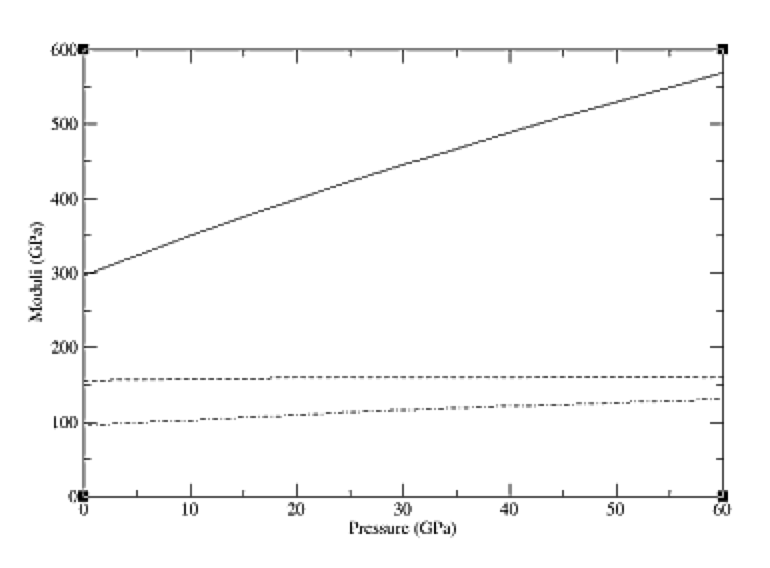
\includegraphics{mgoelastic2}
\end{figure}


When compared to the experimental results of Zha \textit{et al}, the
calculated trend in the value of $C_{11}$ is in good agreement in
that it consistently increases under pressure and approximately doubles
in magnitude by the time that 60 GPa is reached. Unfortunately, the
trends for the other elastic constants are not so good, since the
curve for $C_{12}$ flattens with increasing pressure, rather than
becoming steeper, and the curve for $C_{44}$ passes through a maximum
which is not observed in the experimental data from the aforementioned
group. However, the calculated trends do match the extrapolated behaviour
based upon the results of ultrasonic measurements \cite{MgOUltrasonic}.


\subsection{Born effective charges}

The Born effective charges represent a useful means of characterising
the response of a potential model to perturbations, particularly those
that create an electric field. Increasingly values are becoming available
from \textit{ab initio} techniques for solids through the application
of linear response methods. Hence, this quantity can provide a useful
comparison between the results of formal-charge shell model calculations
and more accurate first principles methods.

One of the first materials for which the Born effective charges were
determined using planewave techniques is $\alpha$-quartz. In Table
\ref{BornchargesQuartz} the values obtained from the shell model
of Sanders \textit{et al} \cite{sandersquartz} are compared with
those yielded by a planewave calculation using the Local Density Approximation
and norm-conserving pseudopotentials \cite{linearresponseQuartz}.

%
\begin{table}
\caption{\label{BornchargesQuartz}Born effective charges (in a.u.) calculated
according to the shell model of Sanders \textit{et al} \cite{sandersquartz}
and from first principles techniques \cite{linearresponseQuartz}.
Values are shown for the asymmetric unit atoms with the approximate
positions of the Si atom at (0.46,0,0) and the O atom at (0.41,0.27,0.11)
in space group 154, with the origin set to (0,0,1/3).}


\medskip{}


\begin{tabular}{|c|ccc|ccc|}
\hline 
 &  & Si &  &  & O & \tabularnewline
\hline
 & 3.122 & 0.0 & 0.0 & -1.406 & 0.368 & 0.252\tabularnewline
Shell model & 0.0 & 3.530 & 0.292 & 0.364 & -1.920 & -0.517\tabularnewline
 & 0.0 & -0.171 & 3.422 & 0.176 & -0.568 & -1.711\tabularnewline
\hline
 & 3.016 & 0.0 & 0.0 & -1.326 & 0.429 & 0.222\tabularnewline
LDA & 0.0 & 3.633 & 0.282 & 0.480 & -1.999 & -0.718\tabularnewline
 & 0.0 & -0.324 & 3.453 & 0.298 & -0.679 & -1.726\tabularnewline
\hline
\end{tabular}
\end{table}
The comparison of the Born effective charge tensors demonstrates that
the oxygen shell model is surprisingly successful at reproducing the
quantum mechanical data, especially in comparison to rigid ion models,
which would yield a diagonal matrix with all components equivalent.
Furthermore, the polarisability of the shell leads to the ions behaving
as partially charged species with realistic magnitudes. Consequently,
this explains why the seemingly unreasonable use of a formal charge
for $Si^{4+}$actually works extremely well in practice. Similar observations
have been previously made for perovskite materials \cite{linearresponseBaTiO3}.


\subsection{Frequency-dependent optical properties}

Ever since the early days of atomistic simulation within the shell
model context it has been routine to calculate the static and high
frequency dielectric constant tensors. Indeed this data has often
been used during the fitting process as well. However, the values
obtained from experiment will always be measured at a particular frequency
and this will never exactly correspond to the limiting values determined
by the direct means of calculation. As described in the background
theory section, it is possible to evaluate the dielectric properties
and refractive indices as a function of radiation frequency for the
gamma point. 

Here we present results for the frequency variation of the dielectric
constant tensor of quartz, shown in Figure \ref{dielectricquartz},
as calculated using the previously mentioned shell model potential
of Sanders \textit{et al} \cite{sandersquartz}. Note that the limiting
values are the same as the ones obtained without reference to the
phonon frequencies. 

In accord with experiment, the dielectric constant decreases slowly
with the frequency of measurement until the highest phonon mode of
quartz - the Si-O stretch - is approached. At frequencies below this
the curve contains considerable variation caused by the discontinuities
when a lattice phonon mode is reached. For simplicity, the curve shown
is for the dielectric constant in the \textit{ab} plane only. The
corresponding curve for the principal tensor component parallel to
the 001 direction is almost identical, except that the limiting values
are slightly different and the positions of the discontinuities due
to coincidence with phonons are displaced to higher frequency.

While the qualitative agreement with experimental data is good, there
is a quantitative discrepancy in the dielectric constant variation.
This is a result of the imperfection of the original fit to the dielectric
data for quartz, though there are also issues concerning the variation
with temperature since the calculations are formally performed at
absolute zero, while the experiment data was measured at 293 K. However,
the use of empirical fitting implies that the interatomic potentials
do partially account for the temperature difference already. At the
lowest measured frequency, the calculated values are an almost perfect
match due to the faster rate of decrease of the dielectric constant
in the experiment data.

%
\begin{figure}
\caption{\label{dielectricquartz}The on-diagonal component of the dielectric
constant tensor for $\alpha$-quartz in the \textit{ab} plane as a
function of frequency of measurement. The solid line represents the
calculated shell model values, while the crosses represent values
estimated from experimental measurements of the refractive index as
a function of frequency.}


\medskip{}


\begin{centering}
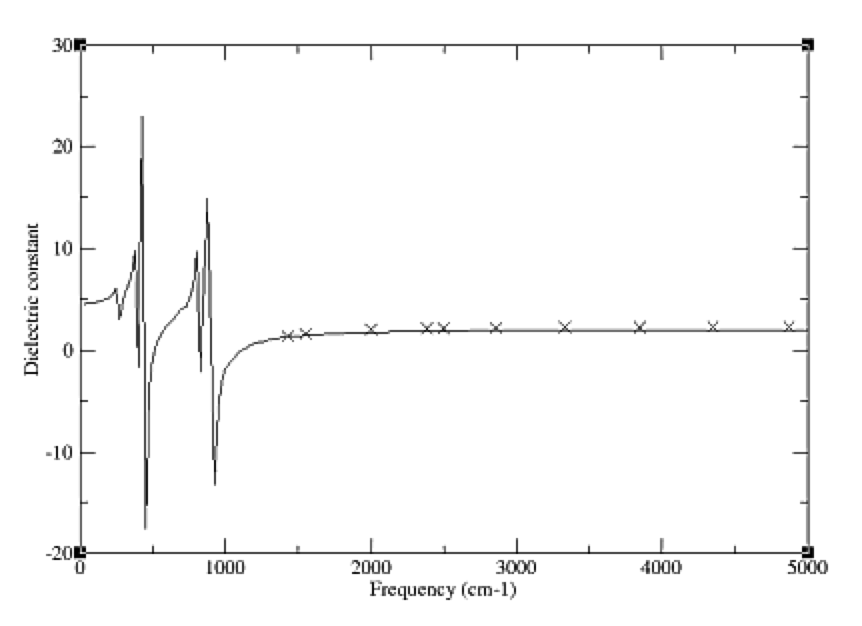
\includegraphics{dielectric2}
\par\end{centering}
\end{figure}



\subsection{Surface calculations}

Before applying GULP to surfaces problems that were previously not
possible, it must first be validated. Firstly, we focus on comparing
our results to MARVIN, starting with the simple inorganic salt corundum.
In the original MARVIN paper \cite{key-106}, the twelve faces with
the lowest interplanar spacings were identified and their surfaces
relaxed using several different potential models. The calculations
utilising the QM5 model were repeated using both MARVIN with the BFGS
minimiser and the same surfaces generated using GDIS and minimised
in GULP using its BFGS minimiser. The unrelaxed surface and attachment
energies were compared and both sets of calculations agreed to better
than $0.0001Jm^{-2}$ for the surface energies and within $0.0001eVmol^{-1}$
for the attachment energies. This indicates that the 2-D Ewald sum
incorporated into GULP is correct. Next the relaxed surface and attachment
energies were compared. Except for the (310) face, all the GULP calculations
returned the same relaxed surface energy as the corresponding MARVIN
run to within $0.0001Jm^{-2}$. The relaxed attachment energies agreed
to within $0.003eVmol^{-1}$. Excluding the (310) face, the MARVIN
calculations took 138 s on a 1133MHz Intel Pentium III CPU Linux system,
whilst the GULP calculations took just 108 s. This difference in timing
is primarily due to the faster energy calculation time in GULP since
the MARVIN minimiser is based on the GULP algorithm and consequently
the number of cycles to minimise a face in GULP and MARVIN only differed
by at most one cycle, except for the (21-1) where GULP took 31 cycles
versus the 24 for MARVIN. The (310) face is interesting as the relaxed
surface energy calculated by GULP is the same as that reported in
the original paper \cite{key-106} and it is the minimised surface
energy from the present calculation with MARVIN that is different.
Although not stated in the MARVIN paper, the minimisations were done
using a combination of minimisers; conjugate gradients until the gradient
norm is unity, followed by a BFGS minimisation. If the MARVIN calculations
are repeated with this combination, all surface energies between MARVIN
and GULP agree to within $0.0001Jm^{-2}$. In conclusion then, we
can say that for this simple inorganic system, GULP and MARVIN produce
essentially the same results.

As an example of the application of the new GULP surface capabilities,
they have been recently utilised to search for surface reconstructions
of the (10-14) cleavage plane of calcite \cite{RohlWrightGale}. The
previous modelling studies have not found any evidence of surface
reconstructions, despite the LEED results of Stipp \cite{Stipp}.
A very efficient and assumption free way of finding reconstructions
is to determine the surface phonon dispersion across the Brillouin
zone, where the presence of any imaginary phonons will indicate that
a reconstruction wants to occur. This calculation was performed on
the cleavage plane of calcite, using a new calcite potential model
that we have recently developed. An imaginary mode was found to be
present at (1/2, 0) in reciprocal space, which indicates that the
system is unstable within the (1x1) surface cell and that the reconstruction
requires the formation of a (2x1) supercell. On creation of the surface
supercell, the system was perturbed along the eigenvector of the imaginary
mode and reminimised using the rational function optimisation technique
to ensure that the final Hessian matrix had the correct character
for an energy minimum. Finally, the optimised (2x1) cell was examined
to ensure that there were no imaginary phonon modes anywhere within
the Brillouin zone. The calculations were repeated using other calcite
models in the literature, which were found not to possess any imaginary
modes. 

In the reconstructed surface, as shown in Figure \ref{calcitesurfaces},
every second row of surface carbonate anions are found to rotate.
The rotation moves the O atom of each carbonate such that it is $13^{o}$
closer to the vertical. This is accompanied by significant change
in the carbonate geometry with an increase of the O-C-O angle of $3^{o}$,
where the two oxygen atoms are those pointing out of the surface and
a compensating decrease in the other two O-C-O angles. Finally, we
note that the reconstruction is confined to the top layer of the surface.
In order to confirm the correct nature of the surface reconstruction,
we have calculated the LEED pattern that would result, which is found
to be an excellent match to the experimental pattern measured by Stipp
under low pressure conditions.

%
\begin{figure}
\caption{\label{calcitesurfaces}Comparison of the geometry for (a) a doubled
unit cell of the (1x1) structure for the (10-14) surface of calcite
and (b) the optimised (2x1) reconstruction of the same surface. The
reconstruction results in every second vertical row, labelled B, adopting
a different configuration to the unreconstructed rows, labelled A.}


\medskip{}


\begin{tabular}{c}
(a)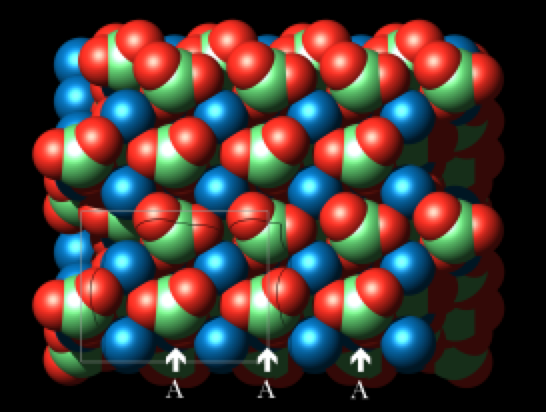
\includegraphics{calcite1}\tabularnewline
(b)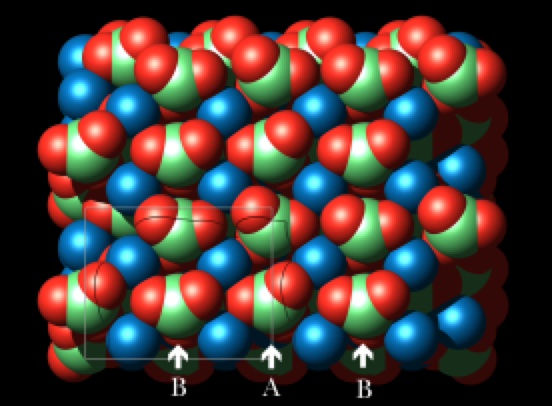
\includegraphics{calcite2}\tabularnewline
\end{tabular}
\end{figure}



\subsection{Bond-order potentials}

Given that new implementation of the Brenner model has been introduced
into GULP we present here some results for diamond, Table \ref{brennerdiamond},
as previously studied in the original paper \cite{key-123}, in order
to validate the code. For the second derivative properties, there
is also the difference that the values obtained here are fully analytic
whereas the published values are obtained via finite differences.
This may explain the small discrepancies in the elastic constants. 

%
\begin{table}
\caption{\label{brennerdiamond}Calculated properties of diamond based on the
model of Brenner \textit{et al} \cite{key-123}. Note that the calculated
values for the bond length and energy are not quoted in the original
reference. However, since the experimental values were part of the
fitted data, we take these values to be equal to the observed ones.}


\begin{tabular}{|c|c|c|c|}
\hline 
Property & Experiment & Original value & GULP value\tabularnewline
\hline
\hline 
Bond length(\AA) & 1.54 & 1.54 & 1.5441\tabularnewline
\hline 
Bond energy (eV) & 3.68 & 3.68 & 3.684\tabularnewline
\hline 
$C_{11}$(GPa) & 10.8 & 10.7 & 10.75\tabularnewline
\hline 
$C_{12}$(GPa) & 1.3 & 1.0 & 1.26\tabularnewline
\hline 
$C_{44}$(GPa) & 5.8 & 6.8 & 7.21\tabularnewline
\hline
\end{tabular}
\end{table}


As stated in the background section, two algorithms have been implemented
for the evaluation of the Brenner potential based on either pairwise
atom looping or a spatial decomposition in order to determine the
neighbour list. The computational cost of the two approaches for increasing
supercells of diamond are illustrated in Figure \ref{brennertimings}.
The linear scaling behaviour of the spatial decomposition can clearly
be seen, as can the fact that this algorithm is effectively superior
in performance for systems containing beyond a 100 atoms. Obviously
this trade off point is dependent on the density of the system, though
there are few cases for hydrocarbons where the density is greater
than that of diamond. For systems much below a 100 atoms the cost
of evaluating the Brenner potential is so negligible in comparison
to other tasks, such as a matrix inversion for property calculation,
that the choice of algorithm is irrelevant.

%
\begin{figure}
\caption{\label{brennertimings}A comparison of the computer times required
for a single energy-force evaluation using the Brenner model according
to whether the algorithm used involves a pairwise sum (solid line)
or a spatial decomposition (dashed line) to evaluate the neighbour
list. Timings given are for a Mac PowerBook G4 laptop with a clock
speed of 700 MHz.}


\begin{centering}
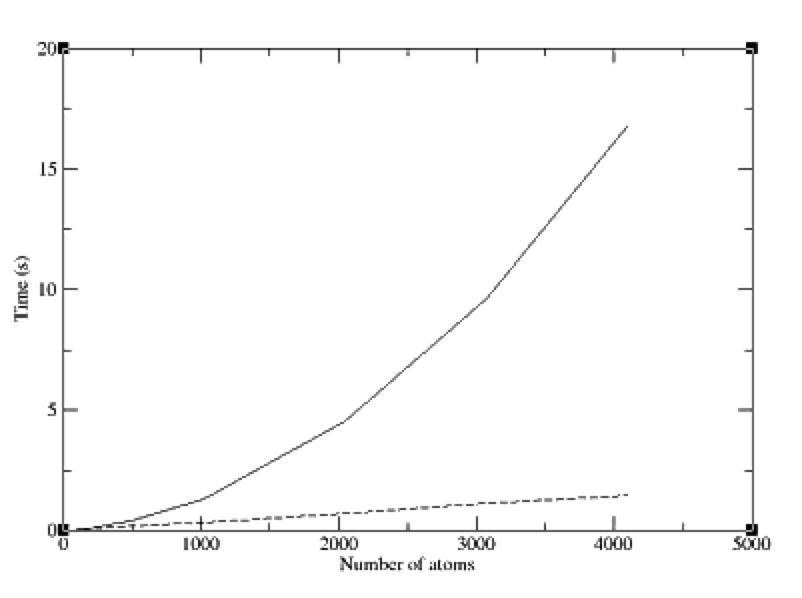
\includegraphics{timebrenner2}
\par\end{centering}
\end{figure}



\chapter{Further background}

In this section some of the theory behind GULP is explained and references
are supplied for those who require a more detailed description of
the methods involved.


\subsubsection{Cut-offs and molecules}

All short-ranged two-, three- and four-bodied potentials have finite
cut-offs in real space which must be set by the user in some way.
Unless the cut-off chosen is so large that convergence is genuinely
achieved then it effectively becomes a parameter of the potential.
Hence when publishing new potentials it is good practice to publish
the cut-offs. Similarly, if you are trying to reproduce the results
of previously published potentials make sure you use the same cut-offs.\\


%
\begin{table}
\caption{\label{tab-gale-twobody} Common functional forms for two-body interatomic
potentials incorporated into GULP (where $r$ represents the distance
between two atoms $i$ and $j$). For full documentation see help.txt.}


\vspace{5mm}

\scalebox{0.8}{
\begin{tabular}{|l|l|l|}
\hline 
Potential Name  &  Formula  &  Units for input\tabularnewline
\hline
Buckingham  &  $A\exp(-r/\rho)-Cr^{-6}$ &  $A$ in eV, $\rho$ in \AA, $C$ in eV\AA$^{6}$\tabularnewline
 &  & \tabularnewline
 Lennard-Jones$^{\dagger}$ &  $Ar^{-m}-Br^{-n}$ &  $A$ in eV\AA$^{m}$, $B$ in eV\AA$^{n}$\tabularnewline
 & or  & \tabularnewline
 &  $\varepsilon(c_{1}(\frac{\sigma}{r})^{m}-c_{2}(\frac{\sigma}{r})^{n})$ &  $\varepsilon$ in eV, $\sigma$ in \AA\tabularnewline
 &  $c_{1}=(n/(m-n))(m/n)^{(m/(m-n))}$ & \tabularnewline
 &  $c_{2}=(m/(m-n))(m/n)^{(n/(m-n))}$ & \tabularnewline
 &  & \tabularnewline
Harmonic$^{\star}$ & $\frac{1}{2}k_{2}(r-r_{0})^{2}+\frac{1}{6}k_{3}(r-r_{0})^{3}+\frac{1}{12}k_{4}(r-r_{0})^{4}$ & $k_{2}$in eV\AA$^{-2}$, $r_{0}$ in \AA\tabularnewline
 &  &  $k_{3}$ in eV\AA$^{-3}$, $k_{4}$ in eV\AA$^{-4}$\tabularnewline
 &  & \tabularnewline
 Morse  &  $D\{[1-\exp(-a(r-r_{0}))]^{2}-1\}$ &  $D$ in eV, $a$ in \AA$^{-2}$, $r_{0}$ in \AA\tabularnewline
 &  & \tabularnewline
 Spring (core-shell)  &  $\frac{1}{2}k_{2}r^{2}+\frac{1}{24}k_{4}r^{4}$ &  $k_{2}$ in eV\AA$^{-2}$, $k_{4}$ in eV\AA$^{-4}$\tabularnewline
 &  & \tabularnewline
Cosh-spring & $k_{2}r^{2}(cosh(\nicefrac{r}{d})-1)$ & $k_{2}$ in eV\AA$^{-2}$\tabularnewline
 &  & \tabularnewline
 General  & $A\exp(-r/\rho)r^{-m}-Cr^{-n}$ &  $A$ in eV\AA$^{m}$, $\rho$ in \AA,\tabularnewline
 &  &  $C$ in eV\AA$^{n}$\tabularnewline
 &  & \tabularnewline
 Stillinger-Weber  & $A\exp(\rho/(r-r_{max}))(Br^{-4}-1)$ &  $A$ in eV, $\rho$ in \AA, $B$ in \AA$^{4}$\tabularnewline
 (sw2)  &  & \tabularnewline
\hline
\multicolumn{3}{||l||}{$^{\dagger}$ combination rules permitted}\tabularnewline
\multicolumn{3}{||l||}{$^{\star}$ $k_{3}$, $k_{4}$ are optional }\tabularnewline
\hline
\end{tabular}}
\end{table}


%
\begin{table}
\caption{\label{tab-gale-threebody} Common functional forms for three-body
potentials incorporated into GULP (where $r$ represents the distance
between two atoms $i$ and $j$, $\theta_{ijk}$ represents the angle
between the two interatomic vectors $i$-$j$ and $j$-$k$). For
full documentation of all the functional forms available see help.txt.}


\vspace{5mm}

\scalebox{0.8}{
\begin{tabular}{|l|l|l|}
\hline 
Potential Name  &  Formula  &  Units for input \tabularnewline
\hline
Stillinger-Weber  &  $K\exp(\rho/(r_{12}-r_{\textrm{max}})+\rho/(r_{13}-r_{\textrm{max}}))(\cos(\theta_{213})-\cos(\theta_{0}))^{2}$ &  K in eV, \tabularnewline
 (sw3)  &  &  $\rho$ in \AA\tabularnewline
 Three-body $^{\dagger}$ &  $\frac{1}{2}k_{2}(\theta-\theta_{0})^{2}+\frac{1}{6}k_{3}(\theta-\theta_{0})^{3}+\frac{1}{12}k_{4}(\theta-\theta_{0})^{4}$ &  $\theta_{0}$ in $^{\circ}$\tabularnewline
 &  &  $k_{2}$ in eVrad$^{-2}$\tabularnewline
 &  &  $k_{3}$ in eVrad$^{-3}$\tabularnewline
 &  &  $k_{4}$ in eVrad$^{-4}$\tabularnewline
 Three-body$^{\star}$ & $\frac{1}{2}k_{2}(\theta_{213}-\theta_{0})^{2}\exp(-r_{12}/\rho)\exp(-r_{13}/\rho)$ &  $k_{2}$ in eVrad$^{-2}$\tabularnewline
 &  &  $\theta_{0}$ in $^{\circ}$, $\rho$ in \AA \tabularnewline
 Axilrod-Teller  &  $K(1+3\cos\theta_{213}\cos\theta_{123}\cos\theta_{132})/(r_{12}r_{13}r_{23})^{3}$ &  $K$ in eV\AA$^{9}$\tabularnewline
 Exponential  &  $A\exp(-r_{12}/\rho)\exp(-r_{13}/\rho)\exp(-r_{23}/rho)$ &  $A$ in eV, $r$ in \AA\tabularnewline
 Urey-Bradley  &  $\frac{1}{2}k(r_{23}-r_{0})^{2}$ &  $k$ in eV\AA$^{-2}$\tabularnewline
 &  &  $r_{0}$ in \AA\tabularnewline
Cosine-harmonic & $\frac{1}{2}k_{2}\left(\cos\theta-\cos\theta_{0}\right)^{2}$ & $k_{2}$in eV\tabularnewline
Linear3 (lin3) & $k(1\pm\cos(n\theta))$ & $k$ in eV\tabularnewline
Hydrogen-bond & $(\frac{A}{r^{m}}-\frac{B}{r^{n}})\cos^{p}\theta$ & A in eV\AA$^{m}$, B in eV\AA$^{n}$\tabularnewline
UFF3 & $K(C_{0}+C_{1}cos\theta+C_{2}\cos2\theta)$ & $K$ in eV\tabularnewline
Equatorial & $\frac{2K}{n^{2}}(1-\cos(n\theta))+2K\exp(-\beta(r_{13}-r_{0}))$ & $K$ in eV, $\beta$ in \AA$^{-1}$\tabularnewline
Bond-angle cross & $\left(k_{1}\left(r_{ij}-r_{ij}^{0}\right)+k_{2}\left(r_{jk}-r_{jk}^{0}\right)\right)\left(\theta-\theta_{0}\right)$ & $k_{1}$$ $ \& $k_{2}$ in eV \AA$^{-1}$deg$^{-1}$ \tabularnewline
(bacross) &  & \tabularnewline
Bond cos cross & $k_{1}\left(r_{ij}-r_{ij}^{0}\right)\left(r_{jk}-r_{jk}^{0}\right)(1+b\cos(n\theta)^{2})$ & $k_{1}$ in eV \AA$^{-2}$\tabularnewline
Bond cross & $\left(k_{1}\left(r_{ij}-r_{ij}^{0}\right)\left(r_{jk}-r_{jk}^{0}\right)\right)$$ $ & $k_{1}$ in eV\AA$^{-2}$\tabularnewline
\hline
\multicolumn{3}{||l||}{$^{\dagger}$ harmonic, option \texttt{three}}\tabularnewline
\multicolumn{3}{||l||}{$^{\star}$ harmonic + exponential, option \texttt{three expo} }\tabularnewline
\hline
\end{tabular}}
\end{table}


%
\begin{table}
\caption{\label{tab-gale-fourbody} Common functional forms for four-body potentials
incorporated into GULP (where $\phi_{ijkl}$ is the torsional angle
between the planes $ijk$ and $jkl$). For full documentation see
the file help.txt.}


\vspace{5mm}

\scalebox{0.8}{
\begin{tabular}{|l|l|l|}
\hline 
Potential Name  &  Formula  &  Units for input\tabularnewline
\hline
Torsion &  $k(1+\cos(n\phi-\phi_{0}))$ &  $k$ in eV, $\phi_{0}$ in $^{\circ}$\tabularnewline
ESFF torsion & $k_{1}\sin_{1}^{2}\sin_{2}^{2}\pm k_{2}\sin_{1}^{n}\sin_{2}^{n}\cos(n\phi)$ & $k$ in $eV$\tabularnewline
 Ryckaert-Bellemans  &  $\sum k_{n}(\cos\phi)^{n}$ &  $k_{n}$ in eV\tabularnewline
Tortaper/torexp & As per torsion multiplied by taper or exponential decay & \tabularnewline
Torharm & $\tfrac{1}{2}k(\phi-\phi_{0})^{2}$ & $k$ in $eVrad^{-2}$, $\phi_{0}$ in $rad$\tabularnewline
UFF4 & $\tfrac{k}{2}(1-\cos(n\phi_{0})\cos(n\phi))$ & $k$ in $eV$\tabularnewline
Torangle & $k\cos(\phi)(\theta_{123}-\theta_{123}^{0})(\theta_{234}-\theta_{234}^{0})$ & $k$ in $eVrad^{-2}$\tabularnewline
Torcosangle & $k\cos(\phi)(\cos(\theta_{123})-\cos(\theta_{123}^{0}))(\cos(\theta_{234})-\cos(\theta_{234}^{0}))$ & $k$ in eV\tabularnewline
Out of plane & $k_{2}d^{2}+k_{4}d^{4}$ & $k_{2}$ in eV\AA$^{-2}$, $k_{4}$ in eV\AA$^{-4}$ \tabularnewline
Inversion & $
k(1-\cos(\phi))$
 & $k$ in eV\tabularnewline
Cross angle (xangleangle) & $k_{213/4}(\theta_{213}-\theta_{213}^{0})(\theta_{214}-\theta_{214}^{0})+$ & $k_{213/4}$ , $k_{312/4}$ , $k_{412/3}$ in $eVrad^{-2}$\tabularnewline
 & $k_{312/4}(\theta_{312}-\theta_{312}^{0})(\theta_{314}-\theta_{314}^{0})+$ & \tabularnewline
 & $k_{412/3}(\theta_{412}-\theta_{412}^{0})(\theta_{413}-\theta_{413}^{0})$ & \tabularnewline
Cross angle cosine (xcosangleangle) & $k_{213/4}(\cos(\theta_{213})-\cos(\theta_{213}^{0}))(\cos(\theta_{214})-\cos(\theta_{214}^{0}))+$ & $k_{213/4}$ , $k_{312/4}$ , $k_{412/3}$ in eV\tabularnewline
 & $k_{312/4}(\cos(\theta_{312})-\cos(\theta_{312}^{0}))(\cos(\theta_{314})-\cos(\theta_{314}^{0}))+$ & \tabularnewline
 & $k_{412/3}(\cos(\theta_{412})-\cos(\theta_{412}^{0}))(\cos(\theta_{413})-\cos(\theta_{413}^{0}))$ & \tabularnewline
UFF out of plane & $k(c_{0}+c_{1}\cos(\phi)+c_{2}\cos(2\phi))$ &  $k$ in eV\tabularnewline
\hline
\end{tabular}}
\end{table}


The main effect of finite cut-offs is to introduce discontinuities
into the energy surface as atoms move across the boundary. Generally
speaking, the energy minimisation procedure in GULP is not too sensitive
to these because of the use of analytical second derivatives. However,
if working with only first derivatives or particularly short cut-offs
this can be the reason for a minimisation failing to satisfy the required
convergence criteria.

An important difference between GULP and some other programs is that
it is perfectly allowable for potentials to overlap, i.e. two or more
potentials can act between the same species at the same distance.
Hence, there are no resulting restrictions for the cut-offs and complex
potential functions can be built by combining several potentials together.
Conversely, it is important not to duplicate potentials when not intended.

For some types of potential the cut-offs may correspond to chemical
criteria such as bond lengths or they may only need to act between
molecules or conversely only within them. In such cases it is best
not to use distance cut-offs to achieve the correct effect, but instead
to use the molecule handling facilities within GULP. There are three
keywords which when specified activate the molecule facility within
the program - \texttt{molecule, molq} and \texttt{molmec}. If any
of these words are present then a search will be performed to locate
any molecules within the structures input. This is done by searching
for bonds based on the sum of the covalent radii plus a percentage
tolerance factor. For most common compounds the default covalent radii
will be sufficient to locate all the bonds - if this is not the case
then it is possible for the user to either increase the tolerance
factor or to adjust the covalent radii using the \texttt{covalent}
option from the \texttt{element} group of commands.

An alternative scenario is that atoms become bonded which shouldn't
be. For example, metal atoms often can become bonded in ionic compounds
because the covalent radii is no longer relevant for a positively
charged ion. These bonds can be removed either by manually setting
the radii of the element to zero or by using the \texttt{nobond} option
to exclude the formation of certain bond types. Whether the correct
molecules have been located or not can be seen from the molecule print
out in the output file. The three molecule-based keywords mentioned
above differ in what they imply for the treatment of intramolecular
electrostatics:\\


\begin{tabular}{llp{10cm}}
 \texttt{molecule} &  $\Rightarrow$ &  exclude all Coulomb interactions within the molecule\tabularnewline
 \texttt{molq} &  $\Rightarrow$ &  retain all Coulomb interactions within the molecule\tabularnewline
 \texttt{molmec} &  $\Rightarrow$ &  exclude all Coulomb interactions between atom which are bonded (1-2)
or two bonds away (1-3)\tabularnewline
\end{tabular}

The specification of \texttt{molmec} does not automatically imply
that all potentials will be treated in a molecular mechanics fashion,
only the electrostatic terms. Providing one of the above three terms
is present then optional words may be added to a potential specification
line which control aspects of the potential cut-offs. When specifying rigid molecules
then it is recommend to use the keywords \texttt{rigid} and \texttt{molecule}. Below is a list
of the words that are available and whether it is necessary to still
give any cut-offs on the potential parameter line:\\


\begin{tabular}{|l|l|l|}
\hline 
Option  &  Effect  &  Cut-offs? \tabularnewline
\hline
\texttt{intra} &  only act within a molecule  &  yes \tabularnewline
\texttt{inter} &  only act between molecules  &  yes\tabularnewline
\texttt{bond} &  only act between bonded atoms  &  no\tabularnewline
\texttt{x12} &  do not act between bonded atoms  &  yes\tabularnewline
\texttt{x13} & do not act between 1-2 and 1-3 atoms & yes \tabularnewline
\texttt{x14} & do not act between 1-2, 1-3 and 1-4 atoms & yes \tabularnewline
\texttt{o14} & only act between 1-4 atoms & yes \tabularnewline
\texttt{g14} & act between 1-4 atoms and beyond & yes \tabularnewline
\texttt{single} & only act where atoms are singly bonded & no\tabularnewline
\texttt{resonant} & only act where atoms are resonantly bonded & no\tabularnewline
\texttt{double} & only act where atoms are doubly bonded & no\tabularnewline
\texttt{triple} & only act where atoms are triply bonded & no\tabularnewline
\texttt{quadruple} & only act where atoms are quadruply bonded & no\tabularnewline
\texttt{amide} & only act where atoms are part of an amide group & no\tabularnewline
\texttt{custom} & only act where atoms are joined by a custom bond & no\tabularnewline
\texttt{half} & only act where atoms are half bonded & no\tabularnewline
\texttt{quarter} & only act where atoms are a quarter bonded & no\tabularnewline
\texttt{third} & only act where atoms are one third bonded & no\tabularnewline
\hline
\end{tabular}

\ \\
In addition to atoms being bonded, GULP now offers the ability to
specify a bond type for each bond. This can be used so a potential
only acts between two species when they have a particular bond order.
At present the bond order has to be specified via the \texttt{connect}
option (see below).

Although with some options it is necessary to still specify a cut-off
for generality, the value may not be important any more. For example,
if an O-H potential for water is specified as being intramolecular
then as long as the maximum distance cut-off is greater than about
1.0 \AA\ then it doesn't matter particularly what it is. Similarly
for a potential which is given as being \texttt{x12} then it doesn't
matter if the minimum cut-off distance is zero - the potential won't
act between bonded atoms. 

By default, GULP dynamically calculates the molecular connectivity
during a calculation. The reason for this is that it ensures that
the restart file will yield the same answer as the point in the calculation
where it left off. However, sometimes difficulties occur because a
bond becomes too long and the molecule breaks into two. When this
happens GULP will stop with an error message as this often indicates
that the potential model is not working well for the system under
study. If the user wants to proceed regardless then there is a keyword
\texttt{fix} which tells the program to fix the connectivity as that
at the starting geometry and not to update it. This means that the
program will never stop with this error, but it does mean that a restart
may not give the same answer as the initial run if atoms have moved
too far. There is now also the option for the user to specify the
connectivity explicitly in the input deck using the \texttt{connect
}option. Note that when using symmetry the \texttt{connect} option
must be specified based on the full cell atom numbers and for all
images at present. 

In the case of ionic materials where the user would like to try to
remove some of the numerical problems associated with cut-offs then
there are some other options. The normal way of doing this is with
a cut-and-shifted potential. In this approach the potential is forced
to go to zero at the cut-off by adding a constant to the energy. This
makes the energy continuous, but the gradient still has a discontinuity.
Again this can be resolved by adding a second term which shifts the
gradient to be zero at the cut-off. In GULP this takes the form of
a linear term in the distance which, provided the cut-off isn't very
short, will have minimal effect in the region of the potential minimum.
These corrections are activated using the potential options \texttt{energy}
or \texttt{gradient} after the potential type, but are only currently
applicable to certain two-body potentials where it is appropriate.
It should be noted that some potential functions go to zero by construction
at the cut-off, for example the Stillinger-Weber two- and three-body
potentials.


\subsubsection{Combination rules}

When using Lennard-Jones potentials it is common to use combination
rules to determine the interaction parameters between two species.
This means that the parameters for the interaction are determined
from one-centre only parameters by some form of averaging. The main
advantage of this approach is that it reduces the number of parameters
to be determined and aids transferability of potentials. Conversely,
the resulting potentials may not be as accurate for any one given
system. There are two types of combination rule used, depending on
whether the potential is being used in the $\varepsilon$/$\sigma$
or A/B format (see Table 2 for details). If the potentials are being
used in the A/B form then the average is taken using a geometric mean:
\[
A_{ij}=\sqrt{A_{i}A_{j}}\]
 \[
B_{ij}=\sqrt{B_{i}B_{j}}\]
 However, if the $\varepsilon$/$\sigma$ form is being employed then
a more complex relationship is needed: \[
\varepsilon_{ij}=\frac{2(\varepsilon_{i}\varepsilon_{j})^{\frac{1}{2}}(\sigma_{i}^{3}\sigma_{j}^{3})}{(\sigma_{i}^{6}+\sigma_{j}^{6})}\]
 \[
\sigma_{ij}=\left(\frac{\sigma_{i}^{6}+\sigma_{j}^{6}}{2}\right)^{\frac{1}{6}}\]


Within GULP it is possible to specify the parameters by species, rather
than by pairs of species, using the \texttt{atomab} or \texttt{epsilon}
options. If the word \texttt{combine} is added to the specification
of a \texttt{lennard}-type potential then the parameters can be omitted
from the input and they will be generated using the appropriate combination
rules. In turn this makes it possible to fit potentials based on combination
rules without having to do this via a series of constraints.


\subsubsection{Mean field theory}

One of the biggest problems that can face someone attempting to simulate
complex materials is the fact that often they can be partly disordered
or involve partial occupancies of sites. One approach to treating
such systems is to generate a supercell so that lots of permutations
can be examined. However, the number of possibilities is usually too
large to examine each one individually to locate the most stable configuration.
Furthermore, this process may alter the symmetry of crystal. Fitting
potentials to such structures also becomes rather difficult.

An alternative approach to handling partial occupancies is to use
mean field theory. The effect of this is that each site experiences
a potential which is the mean of all possible configurations on the
disordered positions. In doing so we are assuming that all possible
configurations are equally as likely, i.e. the less stable configurations
are equally as likely as the more stable ones. This may apply to materials
were there is little energetic difference between configurations or
to ones which were formed under kinetic rather than thermodynamic
control and haven't had the chance to achieve a Boltzmann distribution.
It must be decided for any given material whether it is therefore
appropriate to use this approach.

The practical upshot of the mean field method is that all interactions
just become scaled by the site occupancies of both atoms. This has
been implemented in GULP such that the user can specify the site occupancy
in addition to the coordinates (see the later section on the input
for further details) and the program will automatically handle most
aspects of the mean field approach. This includes ensuring the total
occupancy on a site does not exceed unity and where two different
ions share a site with partial occupancy they are constrained to move
as a single ion in optimisations.

One important word of warning - it is important that the user thinks
through interactions carefully when using the partial occupancy feature
to ensure that everything is handled properly. The biggest danger
comes in systems where there are two partially occupied sites very
close to each other such that in the real system their occupancy would
be mutually exclusive. When this happens it is often necessary to
specifically exclude potentials between these atoms to obtain the
correct behaviour.


\subsubsection{Algorithms for energy and derivative evaluations}

GULP actually contains several different algorithms for calculating
the energy and its first and second derivatives. By default the program
will try to choose the most efficient for any given system, excluding
possibilities such as the cell multipole method which would actually
lead to slight changes in the answer. Normally the user will need
to know nothing about what algorithm is being used, so this section
is really for the curious.

Usually real-space interactions are calculated in a lower-half triangular
fashion to avoid double counting of interactions which would give
rise to loops of the form shown below:\\


\begin{samepage}
\noindent \hspace*{2cm} do \(i\) = 2, \(numat\)\\
\noindent\hspace*{2.5cm}   do \(j\) = 1, \(i\)-1\\
\noindent\hspace*{3cm}  [Calculate interaction between \(i\) and \(j\)]\\
\noindent\hspace*{2.5cm}  enddo\\
\noindent\hspace*{2cm} enddo\\
\end{samepage}

If there is the possibility of self-terms or interactions between
periodic replications of the same atom then the $i=j$ term would
not be excluded, though it may be more efficient to handle this case
in a separate loop. For solids where there is significant space group
symmetry then a different algorithm may be more efficient:\\


\begin{samepage}
\noindent\hspace*{2cm}do \(i\) = 1, \(nasym\)\\
\noindent\hspace*{2.5cm}do \(j\) = 1, \(numat\)\\
\noindent\hspace*{3cm}[Calculate interaction between \(i\) and \(j\)]\\
\noindent\hspace*{2.5cm}enddo\\
\noindent\hspace*{2cm}enddo\\
\end{samepage}

where $nasym$ is the number of species in the asymmetric unit and
$numat$ is the number of atoms in the full unit cell. Both the symmetry
adapted and standard algorithms are present in GULP with selection
being made based on the amount of symmetry in the crystal. The use
of symmetry can result in up to an order of magnitude speed-up in
favourable cases and therefore is well worth using. More details concerning
the use of symmetry, in particular with respect to the calculation
of derivatives, can be found elsewhere {[}11].

The second algorithmic aspect to mention applies to the situation
when a constant volume optimisation is being performed and some atoms
are held fixed. Typical cases where this occurs are in an optical
calculation, in which only shells are relaxed, or where a molecule
is docked within a rigid microporous material. In this case the energy
of interaction between certain atoms is a constant term and the forces
on them are ignored. When this happens these atoms are excluded or
frozen out of the energy calculation after the first point to save
computational expense.


\subsection{Phonons}


\subsubsection{Phonon density of states}

We may also be interested in the phonon density of states for a solid
as the number of frequencies versus frequency value becomes a continuous
function when integrated across the Brillouin zone. While full analytical
integration across the Brillouin zone is not readily carried out,
this integral can be approximated by a numerical integration. We can
imagine calculating the phonons at a grid of points across the Brillouin
zone and summing the values at each point multiplied by the appropriate
weight (which for a simple regular grid is just the inverse of the
number of grid points). As the grid spacing goes to zero the result
of this summation tends to towards the true result.

For performing these integrations GULP uses a standard scheme developed
by Monkhorst and Pack {[}16] for choosing the grid points. This is
based around three so-called shrinking factors, $n_{1}$, $n_{2}$
and $n_{3}$ - one for each reciprocal lattice vector. These specify
the number of uniformly spaced grid points along each direction. The
only remaining choice is the offset of the grid relative to the origin.
This is chosen so as to maximise the distance of the grid from any
special points, such as the gamma point as this gives more rapid convergence.

In many cases it is not necessary to utilise large numbers of points
to achieve reasonable accuracy in the integration of properties, such
as phonons, across the Brillouin zone. For high symmetry systems several
schemes have been devised to reduce the number of points to a minimum
by utilising special points in $k$ space. However, because GULP is
designed to be general the Monkhorst-Pack scheme is used. The user
can input special points instead, if known for the system of interest.

Often it is not necessary to integrate across the full Brillouin zone
due to the presence of symmetry. By using the Patterson group (the
space group of the reciprocal lattice) GULP reduces the integration
region to that of the asymmetric wedge which may only be 1/48-th of
the size of the full volume {[}17].

When producing plots of the phonon density of states the critical
factor, apart from the resolution of the integration grid, is the
`box' size. The continuous density of states curve has to be approximated
by a series of finite regions of frequency or boxes. Each phonon mode
at each point in k space is assigned to the box whose frequency region
it falls into. The smaller the box size the better the resolution
of the plot. However, more points will be needed to maintain a smooth
variation of number density.


\subsubsection{Infra-red phonon intensities}

In order to make comparison between theoretically calculated phonon
spectra and experiment it is important to know something about the
intensity of the vibrational modes. Of course the intensity depends
on the technique being used to determine the frequency as different
methods have different selection rules. While Raman intensities are
not readily calculable from most potential models, due normally to
the absence of polarisabilities higher than dipolar ones, approximate
values for infra-red spectra can be determined {[}18]: \[
I_{IR}\propto(\sum_{\textrm{all}\,\,\textrm{species}}qd)^{2}\]


where $q$ is the charge on each species and $d$ is the Cartesian
displacement associated with the normalised eigenvector.

\subsubsection{Pair Distribution Functions}
The calculation of Pair Distribution Functions is in accordance with the theory of Chung and Thorpe \cite{Chung99}. It makes use of phonon information calculated within GULP, for an optimised structure, using a Monkhorst-Pack grid (as described in section 3.0.28.1). 

Chung and Thorpe \cite{Chung99} state that the probability of finding a pair of atoms~$i$ and~$j$, with position $\mathbf{r}_i$  and $\mathbf{r}_j$  respectively, at position $\mathbf{r}$ is given by
%
\begin{equation}
\rho_{ij}(\mathbf{r})=\left<\delta(\mathbf{r}-(\mathbf{r}_{j}-\mathbf{r}_i) )\right>\label{eqn:rhoij}
\end{equation}
%
where $<\dots>$ is the statistical average implying both configurational and thermal averages.  Summing over all such pairs gives the \emph{density function} $\rho(\mathbf{r})$, which is averaged by using each atom in turn as the starting point. Working with a crystal lattice, the complexity of such calculations is reduced because only atoms in the first unit cell are used as starting points. Moreover, GULP reduces the crystal symmetry to a primitive cell, minimizing the required number of calculations. (It is, of course, still possible to specific a conventional cell and use these k points instead.)

Consider a lattice of unit cells each containing $n$ atoms. Denote the position of atom~$i$ in the original unit cell as $\mathbf{r}_{i_0}$ and similarly atom~$j$ in the $\ell$th unit cell as $\mathbf{r}_{j_\ell}$. Define the pair separation vector between two atoms~$i_0$ (in the original unit cell) and~$j_\ell$ (in the $\ell$th unit cell) as $\mathbf{r}_{i_0j_\ell} = \mathbf{r}_{j_\ell} - \mathbf{r}_{i_0}$. 

The density function (with units of 1/volume) is the weighted sum over all pairs between atom~$i_0$ and atom~$j$ in all unit cells, averaged over the number of atoms in the unit cell, $n$. The spherical average is taken, dividing by $4\pi r^2$, to remove orientational dependence. 
%
\begin{equation}
\rho(r)=\frac{1}{4\pi r^2 n} \sum_{\ell}\left(\sum_{i_0} \sum_{j}^{'} w_{ij} \rho_{i_0j_\ell}(\mathbf{r})\right)\label{eqn:rhor}
\end{equation}
%
where the prime indicates $i_0\not=j_0$ (i.e. $\mathbf{r}_{i_0j_\ell} \not= 0$). The guassian peak (with units of 1/length), is given in equation~\ref{eqn:partialdensityfunction}. The weighting is dependent on the fraction of atoms of type $i$ ,$c_i$, and coherent bound scattering length, $\bar{b}_i$, and is expressed as
%
\begin{equation}
w_{ij} = \frac{\bar{b}_{i}\bar{b}_{j}}{\left(\sum_{k=1}^{n} c_k \bar{b}_k\right)^2}
\end{equation}
%
As suggested by equation \ref{eqn:rhoij}, if the atoms were completely stationary, the density function would be a series of delta functions located at the interatomic spacings. To account for thermal motion, Chung and Thorpe \cite{Chung97} demonstrated that, within the harmonic approximation, the Debye-Waller theorem can be used to justify the use of a series of weighted Gaussian peaks $\rho_{ij}(r)$, centred at $r_{ij}$ with width $\sigma_{ij}$. Taking $\hat{r}_{ij}$ to be the unit vector between atoms $i$ and $j$, and $\mathbf{u}_{ij} = \mathbf{u}_{j} - \mathbf{u}_{j}$ where $\mathbf{u}_{i}$ is the displacement of atom $i$, then the width is given by
%
\begin{equation}
\sigma_{ij} = \left<\left[\mathbf{u}_{ij}\cdot\hat{r}_{ij}\right]^2\right>^{\frac{1}{2}}
\end{equation}
%
This can be expressed in terms of phonon modes as
%
\begin{equation}
\sigma_{i_0j_\ell}^2 = \frac{\hbar}{2N}
\displaystyle\sum_{\mathbf{k},\nu} 
\frac{{\displaystyle 2n\left[\omega(\nu,\mathbf{k})\right]+1}}
{{\displaystyle{\omega(\nu,\mathbf{k}) |\mathbf{r}_{i_0j_\ell}
 |^2}}} |\left[ \mathbf{u}_{j\ell}(\nu,\mathbf{k}) - \mathbf{u}_{i0}(\nu,\mathbf{k}) \right]\cdot\mathbf{r}_{i_0j_\ell}|^2
\end{equation}
%
where the displacements $\mathbf{u}_{i\ell}$ are as given in equation~\ref{eqn:uil}. It should be noted that this corrects a typographical error by Reichard et al \cite{Reichardt01} equation 3, where the numerator is multiplied by a factor of $\sqrt{m_i}$ rather than divided by it.
%
\begin{equation}
\mathbf{u}_{i\ell} = \frac{\mathbf{e^{\mathrm{sig}}}_i(\nu,\mathbf{k})\exp{\left[i\mathbf{k}\cdot\mathbf{r}_{i_\ell}\right]}}{\sqrt{m_i}}
\label{eqn:uil}
\end{equation}
%
$N$ is the number of $\mathbf{k}$-points, $\nu$ is the mode index, $n\left[\omega(\nu,\mathbf{k})\right]$ is the Bose occupation number
%
\begin{equation}
n= \frac{1}{ \left(\exp(\frac{\hbar\omega}{kT}) - 1\right)}
\end{equation}
%
$\omega(\nu,\mathbf{k})$ is the frequency from the eigenvalues of the dynamical matrix, and $\mathbf{e^{\mathrm{sig}}}_i(\nu,\mathbf{k})$ is the eigenvector for atom $i$ (see section~\ref{subsection:eigenvectors}). The mass of atom $i$ is $m_i$. When this is implemented within GULP, a Monkhorst-Pack grid \cite{key-97} of a specified density is used to generate an even distribution of  $\mathbf{k}$-points.

In summary, the Gaussian peak (with units of 1/length) for each pair is calculated from the width
%
\begin{equation}\label{eqn:partialdensityfunction}
\rho_{i_0j_\ell}(r) =\frac{1}{\sqrt{2\pi\sigma_{i_0j_\ell}^2}}\exp{\left[\frac{|\mathbf{r}_{i_0j_\ell}|-r}{2\sigma_{i_0j_\ell}^2}\right]}
\end{equation}
%

These are summed and averaged as in equation~\ref{eqn:rhor}to give the Chung \& Thorpe (1999) density function (with units of 1/volume). The partial density function for atomic pair $ij$ is the contribution from $\rho_i{_0}j{_l}(r)$ for that pair: the sum of all partials is the total density function

\subsection{Eigenvectors}\label{subsection:eigenvectors}

Within the literature, there are two commonly used settings for calculating the dynamical matrix depending on whether the atomic position in the unit cell is included in the eigenvector, or taken out as a phase factor. The default setting in GULP is the same as that used by Lovesey \cite{Lovesey84}, where the eigenvector of atom $j$ at a given $\mathbf{k}$-point is phased by the position of the atom in the unit cell ($\mathbf{r}_{j_0}$). Lovesey \cite{Lovesey84} writes this as $\mathbf{\sigma}$, but we have used $\mathbf{e^{\mathrm{sig}}}$ here to avoid confusion with peak widths. This is the eigenvector used by Chung and Thorpe\cite{Chung97} and here. Lovesey \cite{Lovesey84} also describes an alternative setting, written as $\mathbf{e}$, used in several books e.g. Willis \& Pryor \cite{Willis75} and Dove\cite{Dove93}. The two settings are related by the phase factor shown (from eq. 4.28 in Lovesey \cite{Lovesey84})
%
\begin{equation}\label{eqn:eigenvectors}
\mathbf{e^{\mathrm{sig}}}_j(\nu,\mathbf{k}) = \mathbf{e}_j(\nu,\mathbf{k}) \cdot \exp{\left[i\mathbf{k}\cdot\mathbf{r}_{j_0}\right]}
\end{equation}
%
\subsection{Commonly Used Correlation Functions}\label{subsection:formalism}

A number of different formalisms for PDFs exist in the literature. Keen \cite{Keen01} performed an extensive survey of these and we follow his recommendations. The three main real space correlation functions, $G(r)$, $D(r)$ and $T(r)$ are variously used depending on the purpose. $T(r)$, which scales as $r$ at large $r$, is often used for peak fitting, and for analyzing structural detail at low $r$ (e.g. in amorphous systems). $D(r)$ is similar to $T(r)$, but has a term subtracted that scales with $r$, making it the correlation function of choice for studying mid to high r structural detail. $G(r)$ is also used as it makes the low r peaks prominent. A comparison of the different forms is given by Dove \cite{Dove02}.

Keen \cite{Keen01} writes the density function of Chung and Thorpe \cite{Chung99} as $\rho^{PDF}(r)$. It is the same as that used in the PDFFIT program \cite{Proffen99} as well as by several current workers in this field, e.g. \cite{Billinge93}  \cite{Proffen03}. This real space correlation function tends to $\rho_o$ at high $r$ and is zero below the minimum interpair spacing.  

The PDFFIT program also outputs a \emph{radial distribution function} \cite{Chung97}, also known as a \emph{pair distribution function} \cite{Chung99}, with units of 1/area. It is written as $G^{PDF}(r)$ by Keen \cite{Keen01}, and defined as
%
\begin{equation}
G^{PDF}(r) = 4\pi r \left[\rho^{PDF}(r) - \rho_o\right]
\end{equation}
%
where $\rho_o=\frac{n}{V_{\rm{unit cell}}}$, the average number density (units of 1/volume). While $\rho^{PDF}(r)$ oscillates around the number density, $G^{PDF}(r)$ oscillates around zero. This can be converted to a Keen \cite{Keen01} \emph{total radial distribution function}, $G(r)$, which  has units of area. At values of $r$ less than the minimum interpair spacing, this function tends to $-\left(\sum_{i=1}^nc_ib_i\right)^2$, and to $\infty$ at high $r$.
%
\begin{equation}
G(r) = \frac{G^{PDF}(r) \left(\sum_{i=1}^nc_ib_i\right)^2}{4\pi r\rho_o}
\end{equation}
%
$G(r)$ is often expressed in units of Barns $(1\times10^{-28}~m^2 = 1\times10^{-8}$~\AA$^2)$, but in the GULP output  we use \AA$^2$ to be consistent with the other correlation functions.

The \emph{differential correlation function}, $D(r)$, and \emph{total correlation function}, $T(r)$, are used as part of the ATLAS suit of programs \cite{Soper89}, as used at the ISIS pulsed spallation neutron source, and defined as
%
\begin{eqnarray}
D(r)&=&4\pi r \rho_o G(r)\\
&=&G^{PDF}(r) \left(\sum_{i=1}^nc_ib_i\right)^2\\
T(r) &=& D(r) + 4\pi r \rho_o \left(\sum_{i=1}^nc_ib_i\right)^2 \\ 
&=&\left(G^{PDF}(r)+4\pi r \rho_o \right)\left(\sum_{i=1}^nc_ib_i\right)^2
\end{eqnarray}
%
$D(r)$ and $T(r)$ have units of 1/length.


In addition to the total pair distributions functions written to the .pdfs file, a .pdfs file is produced for every pair-type (root\_pairnumber\_atom1\_atom2.pdfs) containing a selection of partial pair distribution functions. First, the weighted $\rho_ij(r)$ function: the sum of all of these is the total pair distribution function of Chung and Thorpe. Secondly, a weighted version of $g_ij(r)$, which again sums directory to give $G(r)$. Finally, an unweighted (true) $g_ij(r)$, which corresponds to the  $g_ij(r)$ of Keen\cite{Keen01}. This output can be supressed using the $\tt{nopartial}$ keyword.

\subsubsection{Thermodynamic quantities from phonons}

There are a range of quantities that can be readily calculated from
the phonon density of states. The accuracy with which they are determined
though clearly depends on the $k$ points or shrinking factors selected
for the Brillouin zone integration. For systems with large unit cells
a small number of $k$ points, perhaps even the $\Gamma$-point alone,
will be sufficient. However, for those systems with small to medium
unit cells it is important to examine how converged the properties
calculated are with respect to the grid size.

If a phonon calculation is performed then GULP will automatically
print out the relevant thermodynamical quantities. This output depends
partly on whether a temperature has been specified for the given structure.
If the calculation is set for zero Kelvin then only the zero point
energy is output: \[
ZPE=\sum_{k-{\textrm{points}}}w_{k}\sum_{\textrm{all}\,\,\textrm{modes}}\frac{1}{2}h\nu\]
 where $w_{k}$ is the weight associated with the given $k$ point.
In principal, the zero point energy should be added to the lattice
energy when determining the relative stability of two different structures.
However, because the derivatives of the zero point energy are non-trivial
it is normally neglected in an energy minimisation.

For temperatures above absolute zero we can calculate the vibrational
partition function, which in turn can be readily used to calculate
three further properties:\\
 Vibrational partition function: \[
Z_{\textrm{vib}}=\sum_{k-{\textrm{points}}}w_{k}\sum_{\textrm{all}\,\,\textrm{modes}}\left(1-\exp\left(-\frac{h\nu}{kT}\right)\right)^{-1}\]
 Vibrational entropy: \[
S_{\textrm{vib}}=R\ln Z_{\textrm{vib}}+RT\left(\frac{\partial\ln Z_{\textrm{vib}}}{\partial T}\right)\]
 Helmholtz free energy: \[
A=U-TS_{\textrm{vib}}\]
 where \[
U=U_{\textrm{lattice}\,\,\textrm{energy}}+U_{\textrm{vibrational}\,\,\textrm{energy}}\]
 Heat capacity at constant volume: \[
C_{\textrm{v}}=RT\left(2\left(\frac{\partial\ln Z_{\textrm{vib}}}{\partial T}\right)+T\left(\frac{\partial^{2}\ln Z_{\textrm{vib}}}{\partial T^{2}}\right)\right)\]



\subsection{Free energies}

Although the most common methods for studying the properties of materials
as a function of temperature are molecular dynamics and Monte Carlo
simulations, there is an alternative based on static methods within
the quasi-harmonic approximation. This is to directly minimise the
free energy of the system at a given temperature, where the free energy
is calculated from the lattice energy combined with contributions
from the phonons including the entropy and zero point energy.

The advantages of working with free energy minimisation are that MD
simulations are quite expensive due to the need to reduce the uncertainty
by sampling large amounts of phase space. Molecular dynamics and free
energy minimisation are in fact complementary techniques. The latter
approach breaks down at high temperatures as anharmonic effects become
important - typically it works at temperatures up to half the melting
point as a rough guide. Conversely, molecular dynamics is not strictly
valid at low temperatures because the zero point motions and quantum
nature of the vibrational levels is ignored.

Although in principle it is possible to analytically fully minimise
the free energy of a solid, in practice this is extremely difficult
as it requires the fourth derivatives of the energy with respect to
the Cartesian coordinates. Hence, a number of approximations are normally
made - the main one being that the principal effect of temperature
is to expand or contract the unit cell and the effect on internal
degrees of freedom is less important.

When changing unit cell parameters we are concerned with the Gibbs
free energy as this is appropriate to a constant pressure calculation.
This quantity is related to the Helmholtz free energy, whose relationship
to the vibrational entropy has already been given previously, by the
expression; \[
G=A+PV\]
 with \[
P=P_{\textrm{ext}}-P_{\textrm{int}}\]
 where $P$ is the pressure. The pressure has two components - any
external applied pressure plus the internal phonon pressure coming
from the vibrations. The phonon pressure is given by: \[
P_{\textrm{int}}=-\frac{\partial A}{\partial V}\]


In order to calculate the Gibbs free energy it is therefore necessary
to calculate the derivative of the Helmholtz free energy with respect
to the unit cell volume. This can be done numerically by finite differences.
Central differencing is more expensive than using forward differences.
However, it is generally necessary to determine the phonon pressure
with sufficient accuracy. In turn each calculation of the Helmholtz
free energy requires a constant volume minimisation for the given
set of unit cell parameters, followed by a phonon calculation.

Once the Gibbs free energy has been calculated then the next stage
of a free energy minimisation is to isotropically expand or contract
the unit cell until the external pressure balances the internal pressure.
Having done this then the derivatives of the Gibbs free energy can
be evaluated numerically by finite differences and the unit cell optimised
with respect to this quantity.

Because of the three levels of optimisation plus phonon calculations
involved, free energy minimisations are rather expensive and shouldn't
be undertaken lightly! Due to the numerical nature of several of the
derivatives it may be necessary for the user to adjust the finite
differencing interval for a calculation to work optimally. Also the
calculations are very sensitive to the quality of the underlying energy
surface. Potentials with short cutoffs, leading to discontinuities,
and soft modes can cause difficulties for the method, so always check
your model well before starting.

Free energy minimisation can be used in conjunction with fitting to
allow a series of structures at different temperatures to be fitted
with inclusion of the thermal effects, though again this is an expensive
procedure. It is important to note that a free energy minimisation
at 0 K is not the same as an ordinary static calculation. This is
due to the presence of the zero point energy in the former method.


\subsection{Defects}


\subsubsection{The Mott-Littleton method}

The calculation of defect energies is more difficult and approximate
than the calculation of bulk properties. In theory, a defect can cause
very long range perturbations, particularly if it is not charge-neutral.
Consequently the user must always check the convergence of the approximations
made.

The simplification in the modelling of defects is to divide the crystal
that surrounds the defect into three spherical regions known as regions
1, 2a and 2b {[}19-21]. In region 1 all interactions are treated exactly
at an atomistic level and the ions are explicitly allowed to relax
in response to the defect. Except in the case of very short-ranged
defects it is not generally possible to achieve the desired degree
of convergence by increasing region 1 before running out of computer
resources. Consequently, in region 2a some allowance is made for the
relaxation of ions but in a way that is more economical.

In region 2a the ions are assumed to be situated in an harmonic well
and they subsequently respond to the force of the defect accordingly
{[}22]. This approximation is only thus valid for small perturbations
and also requires that the bulk lattice has been optimised prior to
the defect calculation. For region 2a individual ion displacements
are still considered, whereas for region 2b only the implicit polarisation
of sub-lattices, rather than specific ions, is considered.

If the vector $x$ represents the positions of ions in region 1, while
$\zeta$ represents the displacements of ions in region 2a, then the
total energy of the system may be written as: \[
E=E_{1}(x)+E_{12}(x,\zeta)+E_{2}(\zeta)\]
 where $E_{1}$ and $E_{2}$ are the energies of regions 1 and 2 respectively,
and $E_{12}$ is the energy of interaction between them. We now assume
that the energy of region 2 is a quadratic function of the displacements:
\[
E_{2}(\zeta)=\frac{1}{2}\zeta^{T}W\zeta\]


We also know that we wish to obtain the displacements in region 2
for which the energy is a minimum: \[
\frac{\partial E}{\partial\zeta}=0=\frac{\partial E_{12}(x,\zeta)}{\partial\zeta}+W\zeta\]


This expression can be used to eliminate $E_{2}$ from the total energy,
leaving it purely in terms of $E_{1}$ and $E_{12}$: \[
E=E_{1}(x)+E_{12}(x,\zeta)-\frac{1}{2}\frac{\partial E_{12}(x,\zeta)}{\partial\zeta}\zeta\]


The displacements in region 2 are formally a function of $x$ for
region 1 which makes the minimisation of the total energy with respect
to both the positions of region 1 and the displacements of region
2 potentially complicated. This problem can be avoided by using force
balance in region 1 as the criteria for convergence (i.e. all forces
on ions in region 1 must be zero), rather than purely minimising the
energy. The two approaches are equivalent provided that region 2 is
at equilibrium also. This will be achieved provided that the displacements
in region 2 are small enough that they are genuinely quadratic.

In terms of the minimisation procedure employed for defect calculations
the force balance process leads to a slightly different approach to
the bulk optimisation. Initially the same Newton-Raphson procedure
with BFGS hessian updating and line searches is employed to avoid
convergence to stationary points which are not minima. After at least
one cycle of the above and when the gradient norm falls below a certain
threshold the minimiser abandons the line search procedure and aims
purely to reduce the gradients to zero, regardless of the energy.
In practice positive changes in the energy near convergence are only
ever small.

The defect energy is now the difference in the total energies for
the defective and perfect lattice, $E_{d}$ and $E_{p}$ respectively,
with corrections due to the energy of any interstitial or vacancy
species at infinite separation from the lattice, $E_{\infty}$: \[
E_{\textrm{defect}}=E_{d}-E_{p}+E_{\infty}\]


Two final aspects must be dealt with in order to obtain the final
working equations for the defect energy. Firstly, due to the slow
convergence of electrostatic terms in real space alone we cannot evaluate
the region 1 - region 2 energy directly. Instead we must calculate
the energy of region 1 interacting with the perfect lattice to infinity
and then explicitly subtract and add back the terms due to ions which
are no longer on their perfect lattice sites. Secondly, because the
displacements in region 2 depend on the force acting on a given ion,
which in turn is a function of other region 2 ions, there is in fact
a linear dependency of the energy on $\zeta$. By suitable manipulation
of the energy terms this may be removed to leave the following expression
for the defect energy: \begin{eqnarray*}
E_{\textrm{defect}} & = & E_{11}(dd)-E_{11}(dp)+E_{1\infty}(dp)-E_{1\infty}(pp)\\
 &  & +E_{12a}(dd)-E_{12a}(dp)+E_{12a}(pp)-E_{12a}(pd)\\
 &  & -\sum\left(\frac{\partial E_{12a}(dd)}{\partial r}-\frac{\partial E_{12a}(pd)}{\partial r}\right)\end{eqnarray*}


where the general symbol $E_{ij}(kl)$ denotes the energy of interaction
summed over all ions in region $i$ interacting with ions in region
$j$ where $i$ and $j$ can be 1, 2a or $\infty$ (signifying a sum
over 1, 2a and 2b out to infinity). The letters $k$ and $l$ indicate
whether the energy is for the perfect or defective coordinates in
regions $i$ and $j$ respectively, depending on whether they are
$p$ or $d$.


\subsubsection{Displacements in region 2a}

Expanding the energy as a Taylor series and truncating at second order
gives the Newton-Raphson estimate of the vector from the current ion
position to the energy minimum position in terms of the force, $g$,
acting on the ion: \[
\zeta=-W^{-1}g\]


Hence if we know the local second derivative matrix and the force
acting on the ion we can calculate its displacement. There are a number
of possible ways of calculating the force acting on the ions in region
2a. The most common approach is to use the electrostatic force due
to only the defect species - i.e. the force due to any interstitial
species based on their current positions, less the force due to any
vacancies at the position of the original vacant site. In this way
region 2a responds to the change in the multipole moments of the defect
species in region 1, but not the influence of other forces. Hence
for this approximation to strictly hold the distance between any defects
and the boundary of region 2a should be greater than the short-range
cutoff.


\subsubsection{Region 2b energy}

Region 2b is assumed to be sufficiently far from the defects that
the ions only respond by polarising according to the electrostatic
field resulting from the total defect charge placed at the centre
of region 1. This can be written for cubic systems as follows: \[
E_{2b}=-\frac{1}{2}Q^{2}\sum_{i\neq1,2a}\frac{q_{i}m_{i}}{R_{i}^{4}}\]


Because this expression is just dependent on the distance and a couple
of lattice site related parameters the region 2b energy can be evaluated
using a method analogous to the Ewald sum and then subtracting off
the contribution from ions in regions 1 and 2a. An alternative more
general, but still not completely general, expression is the following
where the lattice site dependent property is now an anisotropic tensor,
rather than a scalar {[}23]: \[
E_{2b}=-\frac{1}{2}Q^{2}\sum_{i\neq1,2a}\sum_{\alpha\beta}\frac{q_{i}M_{i}^{\alpha\beta}R_{i}^{\alpha}R_{i}^{\beta}}{R_{i}^{6}}\]
 This can again be calculated by partial reciprocal space transformation
based on the second derivatives of the $R^{-4}$ lattice sum.


\subsection{Fitting}


\subsubsection{Fundamentals of fitting}

Before any production runs can be performed with an interatomic potential
program it is necessary to obtain the potential parameters. If you
are lucky there may be good parameters for your system of interest
already published in the literature so you can just type them in and
get going straight away. Unfortunately most people are not so lucky!
The fitting facility within GULP {[}24] allows you to derive interatomic
potentials in either of two possible ways. Firstly, you can determine
the parameters by fitting to data from some higher quality calculation,
such as an \textit{ab initio} one, normally by attempting to reproduce
an energy hypersurface. Secondly, you could attempt to derive empirical
potentials by trying to reproduce experimental data.

Regardless of which method of fitting you are using the key quantity
is the 'sum of squares' which measures how good your fit is. Ideally
this should be zero at the end of a fit - in practice this will only
happen for trivial cases where the potentials can be guaranteed to
completely reproduce the data (for example fitting a Morse potential
to a bond length, dissociation energy and frequency for a diatomic
should always work perfectly). The sum of squares, $F$, is defined
as follows: \[
F=\sum_{\textrm{all}\,\,\textrm{observables}}w(f_{\textrm{calc}}-f_{\textrm{obs}})^{2}\]
 where $f_{\textrm{calc}}$ and $f_{\textrm{obs}}$ are the calculated
and observed quantities and $w$ is a weighting factor. There is no
such thing as a unique fit as there are an infinite number of possible
fits depending on the choice of the weighting factors. The choice
of weighting factor for each observable depends on several factors
such as the relative magnitude of the quantities and the reliability
of the data (for instance a crystal structure will generally be more
reliable than an elastic constant measurement).

The aim of a fit is to minimise the sum of squares by varying the
potential parameters. There are several standard techniques for solving
least squares problems. By default GULP uses a Newton-Raphson functional
minimisation approach to solving the problem, rather than the more
conventional methods. This is because it avoids storing the co-variance
matrix. The downside is that near-redundant variables are not eliminated.
Currently the minimisation of the sum of squares is performed using
numerical first derivatives. The reason for using numerical derivatives
is because many of the properties, particularly those derived from
second derivatives, are rather difficult to implement analytical derivatives
for. Consequently the value of the gradient norm output during fitting
should only be taken as a rough guide to convergence. In cases where
the numerical gradients prove noisy then the use of the simplex 
algorithm for fitting can be useful as this requires only the function. 

The choice of which potential parameters to fit belongs to the user
and is controlled by a series of flags on the potential input line
(0 $\Rightarrow$ fix, 1 $\Rightarrow$ vary). There are also options
contained within the variables sub-section for allowing more general
parameters to fit, such as charge distributions. Note that when fitting
charges at least two charges must be varied to have any effect as
the program eliminates one variable due the charge neutrality constraint.
There is also the option to vary the charge \texttt{split} between
a core and shell while maintaining a constant overall charge on the
ion. The user may also impose their own constraints on fitting variables
through the \texttt{constrain fit} option.

It is generally recommended that a small number of parameters are
fitted initially and the number gradually increased in subsequent
restarts. Often if all parameters are allowed to vary from the start
unphysical parameters may result. Dispersion terms of Buckingham or
Lennard-Jones potentials are particularly prone to poor behaviour
during fitting, as they tend to go to zero or become exceedingly large.
It is generally recommended that such terms are set equal to a physically
sensible value (based on quantum mechanical estimates or polarisability-based
formulae) and held fixed until everything else is refined.

A final check that the program looks for is that the total number
of variables being fitted is less than the total number of observables!


\subsubsection{Fitting energy surfaces}

To fit an energy surface it is basically necessary to input all the
structures and the energies that correspond to them. To do this it
is just a matter of putting one structure after another in the input
file. It is possible to fit the gradients acting
on the atoms as well the energy of each structure, though often just
the energies are fitted. If the latter is the case, then the easiest
way to turn off the fitting of the gradients is to specify \texttt{noflag}
as a keyword to prevent the program for looking for gradient flags
in the absence of a keyword to specify them.

Perhaps the only unique feature of fitting an energy surface is the
need to include an energy shift in some cases. This is a single additive
energy term which is the same for all structures and just moves the
energy scale up and down. The justification for this is that often
it is impossible to calculate the energy that corresponds exactly
to the interatomic potential one from a quantum mechanical calculation
{[}25]. Most commonly this arises where the potential model has partial
charges in which case there is an unknown term in the lattice energy
due to ionisation potentials and electron affinities for fractions
of an electron.

To simplify the specification of this shift value in the input, if
you give the \texttt{shift} option after the first structure then
this value will apply to all subsequent structures until a different
value is input. Similarly, its magnitude can be altered by using the
\texttt{variables} sub-section to specify the shift as a variable
and this will apply to all structures. It is generally recommended
that the shift is fitted first and allowed to fit through out the
procedure.


\subsubsection{Empirical fitting}

An alternative to fitting quantum mechanical data to derive an interatomic
potential is to actually fit experimental data. In this case the procedure
serves two purposes. Firstly, the degree to which all the data can
be reproduced may serve as some guide as to the physical correctness
of the model used. Secondly, it provides a means of extrapolation
of experimental data for one system to a different one where the data
may not be known, or alternatively to unknown properties of the same
material.

Any of the properties that can be calculated for the bulk solid or
gas phase molecule can also be used in reverse to fit a potential
to. Obviously the essential ingredient in the fit is the experimental
structure, without which you won't get very far! The conventional
way to fit the structure is by requiring that the forces on the atoms
are zero. This is clearly not a perfect strategy as it could be satisfied
by a transition state rather than a minimum, though in practice it
is rare, except when symmetry constraints are imposed.

Normally a good fit requires some second derivative information as
well as the structure. For very high symmetry systems, such as rock
salt, the structural data alone is completely inadequate. If we imagine
a potential as being a binomial expansion about the experimental geometry,
then unless the first and second derivatives are reasonably well reproduced
by our model then the range of applicability will be almost zero.
Typical sources of second derivative information are elastic, dielectric
and piezoelectric (where applicable) constants. Also vibrational frequencies
contain far more information than any of the above. However, the fitting
of frequencies is not straightforward. To fit the frequency magnitudes
is certainly possible, however, you have no guarantee that the correct
mode has been fitted to the correct eigenvalue. Hence, frequency fitting
only tends to be useful from empirical data for special cases, such
as O-H stretching modes which are well separated from other modes
and for diatomics where there is no problem in assignment!

One other case where frequency fitting can be useful is at the lower
end of the spectrum. For an isolated molecule or a solid at its $\Gamma$
point the first three modes should have zero frequency as they are
just translations. In some cases there may be imaginary modes due
the potentials not correctly reproducing the true symmetry. Hence
by fitting the first three modes to be zero it is possible to encourage
the potentials to yield the correct symmetry.


\subsubsection{Simultaneous fitting}

There is one main difficulty in the conventional scheme for fitting
in which the forces on the atoms are minimised by variation of the
potential parameters which arises when using a shell model. Normally
we don't know what the shell coordinates are at the outset unless
the ions are sited at centres of symmetry. In the past people have
tried fitting with the shells placed on top of the cores. However,
this means that the potentials are tuned to minimise the polarisation
in the system and leads to the shell model having only a small beneficial
effect. It also doubles the number of observables connected with gradients,
but only introduces a small number of extra variables thus making
it harder to get a good fit.

The solution to this problem is allow the shell positions to evolve
in some way during the fit. There are two possibilities - either we
can minimise the shell positions at every point during the fit or
we can added the shell coordinates as fitting parameters. In the case
where only structural data is being fitted the two methods are equivalent
except in the way that they evolve towards the answer. When other
properties are included the second approach is not strictly correct,
though the difference is usually small.

After experimenting with several test cases it was found that the
second scheme in which the shell coordinates become fitted variables
was far more stable in convergence and more efficient. Hence this
is the scheme that has been adopted and is referred to as 'simultaneous'
fitting due to the concurrent fitting of shell positions. Whenever
working with shell models it is recommended that the keyword \texttt{simultaneous}
is added during conventional fitting - it can improve the sum of squares
by several orders of magnitude! Not only does this scheme apply to
the coordinates of shells, but also to the radii of breathing shells
as well.


\subsubsection{Relax fitting}

It has been observed that sometimes in conventional fitting getting
an improved sum of squares doesn't always get you what is considered
to be a better quality fit. This is because people often use different
criteria to make their judgement to the ones input into the fitting
process. In particular they look at the difference between the optimised
structural parameters and those from experiment, rather than looking
at the forces. The reason why the forces can be lower, but lead to
a worse structure is because in a harmonic approximation the displacements
in the structure are given by the gradient vector multiplied by the
inverse hessian. Hence, if the gradients get smaller but the inverse
hessian gets much larger then the situation may get worse.

The solution to this problem is to fit according to the criteria by
which the structures are judged - this is what relax fitting does.
This means that at every point in the fit the structure is optimised
and the displacements of the structural parameters calculated instead
of the gradients. In this approach the shell model is naturally handled
correctly and so there is no need for simultaneous fitting. The downside
is that it is much more expensive in computer time than conventional
fitting. Also you can only start a relax fit once you have a reasonable
set of potential parameters - i.e. one which will give you a valid
minimisation. Hence a conventional fit is often a prerequisite for
a relax fit.

There is a further benefit to using relax fitting. In a conventional
fit the properties are calculated at the experimental structure normally
with non-zero gradients which is not strictly correct. In a relax
fit the properties are calculated for the optimised structure where
they are valid.


\subsection{Genetic algorithms}

Conventional minimisation techniques based upon methods such as Newton-Raphson
are excellent ways of locating local minima. However, they are of
limited use in finding global minima. For example, if we know the
chemical composition of a compound and its unit cell, but don't know
the structure then we would want to locate the most stable arrangement
for placing the atoms within the unit cell. To search systematically
for a reasonable set of atomic coordinates may take a very long time
by hand. Genetic algorithms {[}26] are a method by which we can search
for global minima rather than local minima, though there can never
be an guarantee of finding a global minimum. In many respects it resembles
Monte Carlo methods for minima searching, though is regarded by some
as being more efficient.

The concept behind the method, as the name might suggest, is to carry
out a 'natural selection' procedure within the program in the same
way that nature does this in real life. We start off with an even
numbered sample of randomly chosen configurations. This is our trial
set which is allowed to evolve according to a number of principles
described below. Before we can do this we need to consider how to
represent our data for each configuration. To do this we encode each
number as a binary string by dividing the range between the maximum
and minimum possible values (for example 1 and 0 for fractional coordinates)
into a series of intervals where the number of such intervals is an
integer power of 2. Given this data representation the system now
evolves according to the following steps:\\


\noindent \textbf{(a) Reproduction (tournament)} - pairs of configurations
are chosen at random and the parameters which measure the relative
quality of the two are compared (this is the energy for genetic optimisation
or the sum of squares for genetic fitting). The best configuration
goes forward to the next iteration, except that there is a small probability,
which can be set, for the weaker configuration to win the tournament.
This process is repeated as many times as there are configurations
so that the total number remains constant.\\


\noindent \textbf{(b) Crossover} - a random point is chosen at which
to split two binary strings, after which the two segments are swapped
over.\\


\noindent \textbf{(c) Mutation} - a random binary digit is switched
to simulate genetic mutations. This can help to search for alternative
local minima.\\


The default output from a genetic algorithm run is a given number
of the final configurations, where the ones with the best fitness
criteria are selected. However, unless the run smoothly progresses
to the region of a single minimum it may be more interesting to look
at a sample of the best configurations from the entire run. This can
be done with GULP using the \texttt{best} option.

Genetic algorithms can only locate minima to within the resolution
allowed by the discretisation used in the binary representation. Also
they are very slow to converge within the region of a minimum. Hence,
the genetic algorithm should be used to coarsely locate the regions
associated with minima on the global surface, after which conventional
Newton-Raphson methods will most efficiently pin-point the precise
minimum in each case.

\newpage



\section{Getting started}


\subsection{Setting environment variables}

In previous versions of GULP it was necessary to specify where library
files and the documentation could be found by editing the source code.
This has now been replaced by the use of two environment variables,
GULP\_LIB and GULP\_DOC, respectively. Under tcsh these can be set
as follows:\\


\texttt{setenv GULP\_DOC /Users/myname/gulp6.2/Docs}

\texttt{setenv GULP\_LIB /Users/myname/gulp6.2/Libraries}~\\
\texttt{}~\\
or by using appropriate commands under other Unix shells.


\subsection{Running GULP}

Under UNIX:\\
 To run GULP on a machine with the UNIX operating system simply type:\\


\noindent \texttt{<directory>gulp < inputfile} \\


\noindent where \texttt{<directory>}  is the path name for the location
of gulp on your machine, or if the executable is in your current directory
or lies in your path then this may be omitted. In this case the output
will come to your terminal. If you wish to save it to an output file
then type\\


\noindent \texttt{<directory>gulp < inputfile > outputfile}\\


\noindent You may like to try using one of the example input files
(called exampleN, where N is a number) to see what happens! Input
may also be typed directly into the program line by line if no input
file is specified. Having finished typing all the required input just
type `start' to commence the run.\\

\noindent If running in parallel, then it is recommended to use a different
syntax to run GULP:

mpirun -np 4 gulp inputfile

Here mpirun is the command that launches a parallel job under MPI, 4 represents the number of cores
on which to run (for example - other numbers up to the available number of cores are allowed) and
inputfile here represents the name of your inputfile BUT without the .gin extension at the end. This will
be added automatically and the output written to a file with the same root name, but with .gout at the end.
Using this form of running GULP, as opposed to re-directing I/O with < and >, is better in parallel since
it avoids a possible MPI error message relating to not being able to read the input fast enough. 

\subsection{Getting on-line help}

To obtain on-line help on GULP type\\


\noindent \texttt{<directory>gulp <CR>}~\\
\texttt{ help <CR>}~\\


A list of all the possible help topics can then be accessed by typing
\texttt{topics} or alternatively just type the particular keyword
or option that you require help on. Only sufficient characters to
specify a unique topic are required. To finish with help type \texttt{stop}
if you wish to exit the program or \texttt{quit} if you want to return
to interactive use.

If the help command fails to work it means that the path for the location
of the file help.txt (which is an ordinary ASCII text file containing
all the help information) has not been set at compile time and that
the file is not in the present directory either.

An alternative way of accessing help is to generate an HTML file using
the gulp2html utility (courtesy of Dr. Jörg-R. Hill) which produces
a file help.html which can then be inspected with a suitable browser,
such as netscape.


\subsection{Example input files}

With the program you should have received a number of sample input
files which illustrate how GULP works for a number of particular run
types. They also serve as a test to ensure that the program works
correctly on your machine type. Please note that the interatomic potentials
should not be taken as correct for general use - some are made up
for the purposes of demonstration only! Below is a brief description
of what each example file is doing.

\begin{longtable}{|l|p{15cm}|}
\caption{List of examples provided}\\
\hline
\hline
example1 &optimises the structure of alumina to constant pressure and then 
calculates the properties at the final point\\
example2 &simultaneous fit of a shell model potential to the structure of \(\alpha\)-quartz, followed by an optimisation with the fitted potentials - 
the general potential is used with energy and gradient shifts for 
the Si-O instead of the usual Buckingham potential\\
example3&an electronegativity equalisation calculation is used to derive 
partial charges for quartz and are then used to calculate the 
electrostatic potential and electric field gradients at each site - 
bond lengths are also calculated\\
example4&simultaneous fit of a shell model potential to La2O3 using an 
Ewald-style sum to evaluate the C6 terms, followed by an 
optimisation with the production of a table comparing the initial 
and final structures at the end\\
example5 &calculation of a phonon dispersion curve for MgO from 0,0,0 to 
1/2,1/2,1/2 - note that normally the structure should be 
optimised first and that although a phonon density of states 
curve is produced this may not be accurate due to restricted 
sampling of k space.\\
example6 &calculation of the defect energy for replacing a Mg2+ ion in MgO 
by a Li+ ion to create a negatively charged defect\\
example7a&location of the transition state for a magnesium cation migrating 
to a vacant cation site in MgO in a defect calculation\\
example7b&this shows an alternative way of obtaining the same result as in 
7a by starting the magnesium in a special position and using the 
resulting symmetry constraints to allow a ordinary minimisation 
to the saddle point\\
example8&a molecular defect calculation in which a sulphate anion is 
removed from BaSO4 - note that the use of the {\texttt{mole}} keyword to 
Coulomb subtract within the sulphate anion.\\
example9&an example of how to use a breathing shell model for MgO - 
including fitting the model, optimising the structure and 
calculating the properties \\
example10&optimisation of urea showing how to handle intermolecular 
potentials\\
example11&an example of how to map out the potential energy surface for 
the migration of a sodium cation parallel to the c axis through a 
crystal of quartz with an aluminium defect using the translate 
option\\
example12&optimisation of two structures within the same input file - also 
illustrates the use of the name option\\
example13&shows how to use a library to access potentials for an 
optimisation of corundum\\
example14&relaxed fit to structure and properties \\
example15&simple NVE molecular dynamics\\
example16&example of constant pressure shell model MD\\
example17&Sutton-Chen calculation for bulk Ni with cutmany = 1.0 (old default)\\
example17&Sutton-Chen calculation for bulk Ni with cutmany = 0.5 (new default)\\
example18&example of shell model MD in NVT ensemble\\
example19&shell model MD run for a zeolite with finite mass\\
example20&shell model MD run for a zeolite with adiabatic algorithm\\
example21&charged defect optimisation in a supercell\\
example22&energy surface fit for a molecular crystal\\
example23&evaluation of the cost function for a particular structure\\
example24&example of structure prediction for polymorphs of TiO2\\
example25&free energy minimisation of quartz within the ZSISA approximation\\
example26&Using the "ditto" option to run the same structure at 3 pressures in the same file\\
example27&Interface calculation in which a rigid block of MgO is optimised over the 001 surface of MgO\\
example28&Tersoff model calculation on bulk silicon followed by a vacancy defect calculation\\
example29&Streitz-Mintmire model calculation on bulk alumina\\
example30&REBO model calculation for a diamond surface\\
example31&Constant pressure optimisation of a corundum slab with a 2-D phonon calculation\\
example32&1-D calculation on MgO using manual specification of flags and the switch minimiser option\\
example33&Grand Canonical Monte Carlo for a single species being introducted into a box\\
example34&Grand Canonical Monte Carlo for a rigid molecule being introducted into a box\\
example35&Voter-Chen EAM for Ag\\
example36&Frequency dependent property calculation for quartz\\
example37&SiH4 molecule using the Smith and Dyson REBO 1 model\\
example38&Electric field applied to a slab from example31\\
example39&Glue potential for Au with print out of EAM atomic densities and energy contributions\\
example40&Simple example of 3coulomb potential for a water molecule for validation\\
example41&Force calculation for a urea molecule in the presence of a continuum solvent model with qsas keyword\\
example42&Optimisation of the (001) surface of urea in the presence of a continuum solvent model\\
example43&Example of PDF calculation for MgO - phonons < wmax\\
example44&Example of PDF calculation for MgO - full phonon range\\
example45&Example of PDF calculation for MgO - phonons > wmin only\\
example46&Example of PDF calculation for (Ca,Sr)TiO3\\
example47&Example of Eckart keyword for removing rotation/translation from molecular vibrations\\
example48&Fitting of vibration modes using specific eigenvectors for a water molecule\\
example49&UFF input file with manual specification of bonds for meta-xylene\\
example50&Example of Dreiding input\\
example51&Example of a thermal conductivity calculation for Allen-Feldman diffusons in amorphous silicon\\
example52&Example of a thermal conductivity calculation that uses estimated B and v\_s from properties\\
example53&Calculation of Raman intensities for the vibrations of alpha-quartz\\
example54&Example of ReaxFF for an ethene molecule\\
example55&Example of a MEAM-2NN calculation for FCC Cu metal\\
example56&Example of an input for the ZBL potential that uses default parameters\\
example57&Example of a Hessian calculation for Tersoff ZRL. Geometry is chosen so that the coordination term is non-zero\\
example58&As per example57 except using finite differences to compute a numerical Hessian matrix for validation\\
example59&Example of the use of the mcswap option for exchanging Si and Ge in a zeolite\\
example60&Example of the use of multiple mcswap options for exchanging Si/Ge and O/S in a hypothetical zeolite\\
example61&Example of harmonic estimate for energy of relaxation\\
example62&Example of a phonon calculation using force constant supercell computed for a supercell of urea\\
example63&Example of the calculation of mean-squared displacements for the vibrations of a diatomic molecule\\
example64&Example of the calculation of Grueneisen parameters for MgO with a shell model\\
example65&Example of using the scan\_cell option to shear MgO\\
example66&Example of split bond EEM calculation with multiple ranges for Li2O using MEAM\_2NN\_QEq\\
example67&Example of thermal conductivity calculation for MgO using the Alamode-GULP interface to solve the BTE\\
example68&Example of the use of finite strain optimisation relative to a reference cell for alumina\\
example69&Example of MD using multiple temperature ramps to anneal a system\\
example70&Example of a calculation using point ion dipolar polarisability without coupling of dipoles\\
example71&Example of summing shell gradients on to core during fitting\\
example72&Example of calculation an energy for an ion in the presence of non-interacting Langevin dipoles with ML\_BOP water\\
example73&Example of a rigid molecule calculation on paracetamol\\
example74&Example of a rigid molecule optimisation of urea under pressure using the cell parameters instead of strains\\
example75&Example of a rigid molecule optimisation for a monoclinic organic crystal with a taper\\
example76&Example of a rigid molecule calculation for a surface\\
example77&Use of Tersoff potential of Munteh et al for quartz\\
example78&Example of Monte Carlo with a 2-D triangular lattice of spins and species swaps to flip spins\\
example79&Example of using synchronous transit to find a transition state\\
example80&Example of a pGFNFF calculation for graphene\\
example81&Example of a pGFNFF optimisation and property calculation for MOF-5\\
example82&Example of a pGFNFF calculation for HfS2 combined with lowering of the symmetry and removal of imaginary modes\\
example83&Example of using the AA-CLP method of Gavezzotti to compute the lattice energy of a molecular crystal\\
example84&Example of an optimisation of quartz with ReaxFF followed by a phonon calculation using analytic second derivatives\\
example84&Example of an optimisation of quartz with ReaxFF followed by property calculation including charge derivatives\\
\hline
\hline
\end{longtable}


\section{Guide to input}


\subsection{Format of input files}

On the whole it is only necessary to use up to the first four letters
of any word, unless this fails to specify a unique word, and the input
is not case sensitive as all characters are converted to lower case
on being read in.

The first line of the input is the only special line and is referred
to as the keyword line. Keywords should all be given on this line.
These consist of control words which require no further parameters
and generally specify the tasks to be performed by the program. For
example a typical keyword line would look like:\\


\noindent \texttt{optimise conp properties phonon} \\


\noindent or in abbreviated form:\\


\noindent \texttt{opti conp prop phon}\\


This combination of words tells GULP to do a constant pressure optimisation
and then to calculate the lattice properties and phonons at the optimised
geometry. The order of words within the keyword line is not significant.

All subsequent lines can be given in any order unless that line relates
to a previous piece of input. Such lines contain `options' which generally
also require the specification of further information. This information
can normally follow on the same line or on the subsequent line. For
example the pressure to be applied to a structure could be input as
either\\


\noindent \texttt{pressure 10.0} \hspace{2cm} or \hspace{2cm} \parbox[t]{30mm}{\texttt{pressure}~\\
\texttt{ 10.0}~\\
}\\


\noindent In many cases the units may also be specified if you don't
wish to use the default:\\


\noindent \texttt{pressure 1000 kbar}\\


Any lines beginning with a `\#' and anything that follows a `\#' part
way through a line is treated as a comment and as such is ignored
by the program.

When performing runs with multiple structures any structure dependent
options are assumed to apply to the last structure given, or the first
structure if no structure has yet been specified. Some options should
be specified as sub sections of a particular option. For example,
\texttt{elastic, sdlc, hfdlc, piezo, energy} and \texttt{gradients}
all are sub sections of the \texttt{observables} command and should
appear as follows:\\


\noindent \texttt{observables}~\\
\texttt{elastic 2}~\\
\texttt{1 1 54.2}~\\
\texttt{3 3 49.8}~\\
\texttt{hfdlc}~\\
\texttt{1 1 2.9}~\\
\texttt{end}~\\


Provided there is no ambiguity, GULP will accept these options even
if \texttt{observables} is omitted, however, it makes the input more
readable if the section heading is included.

GULP reads only the first 80 characters on a line in an input file.
Should an input line be two long to fit within this limit then the
line can be continued on a second or further lines by adding the continuation
character `\&' to the end of the line.


\subsection{Atom names}

Many parts of the input to GULP require the specification of atom
names, be it when giving their coordinates or when specifying potential
parameters. The convention adopted in GULP is that an atom should
be referred to by its element symbol, optionally followed by a number
to distinguish different occurrences of the same element. Numbers
between 1 and 999 are valid numbers. Hence examples of valid atom
specifiers are \texttt{Si}, \texttt{Si12, O3} and \texttt{H387}. Something
like \texttt{Si4+} would not be a valid symbol. The reason for using
the element symbol is because several calculations use elemental properties
such as the mass or covalent radii in dynamical or molecular runs,
respectively.

Sometimes it is desirable to label all the atoms in the structure
with numbers to identify them, but with the same interatomic potential
acting on them. To avoid having to input the potential multiple times
for each symbol there is a convention within GULP which it is important
to know. Any reference to just an atomic symbol applies to all occurrences
of that element, whereas any reference to an atom type with a number
only applies to that specific species. For example a Buckingham potential
specified as follows:\\


\noindent \texttt{buck}~\\
\texttt{ Si core O core 1283.0 0.299 10.66 0.0 12.0}\\


\noindent would apply to all Si atoms, regardless of whether they
are called \texttt{Si} or \texttt{Si1} etc. However, the following
potential:\\


\noindent \texttt{buck}~\\
\texttt{ Si1 core O core 1283.0 0.299 10.66 0.0 12.0}~\\


\noindent would only act on \texttt{Si1}. It is important to remember
this as people have labelled one atom \texttt{Si} and the \texttt{Si1}
in the past and put potentials for both which resulted in twice the
potential acting on \texttt{Si1} as there should have been. If the
potential had been specified as just acting on \texttt{Si} then the
correct answer would be obtained as it would act on both atoms once.

In addition to the atom label there is optionally a species type specifier
which should be one of the following:\\


\begin{tabular}{ll}
 \texttt{core} &  - represents the main part of an atom including all its mass\tabularnewline
 \texttt{shel} &  - represents the mass-less component in a shell model\tabularnewline
 \texttt{bcor} &  - a core, but with a spherical breathing radius\tabularnewline
 \texttt{bshe} &  - a shell, but with a spherical breathing radius\tabularnewline
\end{tabular}

\ \\


If not given, then \texttt{core} is the default type. Note that the
\texttt{bcor} and \texttt{bshe} types only need to be used in the
structure specification. There after they can be treated as an ordinary
core or shell in the potential specification and the program will
select whether the potential should act on the radius or the centre
of the species.


\subsection{Input of structures}

The structure for a three-dimensional solid requires the input of
three main sets of information - the unit cell, the fractional coordinates
and types of the atoms, and finally the space group symmetry. Taking
these in order, the unit cell can be input either as the cell parameters:\\


\noindent \texttt{cell}~\\
\texttt{ 4.212 4.212 4.212 90.0 90.0 90.0}~\\


\noindent or as the cell vectors:\\


\noindent \texttt{vectors }~\\
\texttt{ 4.212 0.000 0.000}~\\
\texttt{ 0.000 4.212 0.000}~\\
\texttt{ 0.000 0.000 4.212}~\\
\texttt{ }

Normally it is easiest to use the cell parameter form and this is
recommended. The main reason why you might chose to use the cell vectors
is because you want to calculate the properties in a non-standard
reference frame (given that quantities such as the elastic constants
depend on the unit cell orientation relative to the Cartesian frame).
If the cell parameters are input, then the $a$ cell vector is aligned
along the $x$ axis, the $b$ cell vector in the $xy$ plane and the
$c$ cell vector in the general $xyz$ direction.

If the keywords conp or conv are not specified, then the program will
expect 6 flags to indicate how the unit cell is to be optimised. Here
a flag of 1 implies that a degree of freedom should be allowed to
vary and 0 will imply that it should be kept fixed. Because GULP works
with the strain tensor, these flags refer to the strain components
in the order xx, yy, zz, yz, xz and xy, respectively. Examples of
how to input the flags for the case given above when only the on-diagonal
strain components are to be varied are given below:\\


\noindent \texttt{cell}~\\
\texttt{ 4.212 4.212 4.212 90.0 90.0 90.0 1 1 1 0 0 0}~\\


\noindent or as the cell vectors:\\


\noindent \texttt{vectors }~\\
\texttt{ 4.212 0.000 0.000}~\\
\texttt{ 0.000 4.212 0.000}~\\
\texttt{ 0.000 0.000 4.212}~\\
1 1 1 0 0 0\\


When GULP transposes a system between the primitive and centred unit
cells the orientation of the atoms is preserved so that any properties
calculated will be the same regardless of the cell used. It is recommend
that the cell parameters be used for input where possible as this
ensures that symmetry can be used to accelerate optimisations. Turning
now to the internal coordinates of the atoms, these can again be given
either in fractional or Cartesian form, though the former is the more
natural for a periodic system. Each line of input must contain at
least the atom label followed by the coordinates, in which ever units.
For example for the case of MgO:\\


\noindent \texttt{fractional}~\\
\texttt{ Mg core 0.0 0.0 0.0}~\\
\texttt{ O core 0.5 0.5 0.5}~\\
\texttt{ }

Note that if the space group symmetry is to be given then it is only
necessary to specify the atoms of the asymmetric unit. Furthermore
in any cases where a fractional coordinate is a recurring decimal,
such as 1/3, then it is necessary to specify this value to six decimal
places to be sure of it being recognised correctly as a special position.
If we were to include a shell model for oxygen then the input of coordinates
would now look like the following:\\


\noindent \texttt{fractional}~\\
\texttt{ Mg core 0.0 0.0 0.0}~\\
\texttt{ O core 0.5 0.5 0.5}~\\
\texttt{ O shel 0.5 0.5 0.5}~\\
\texttt{ }

There is no need to specify the number of atoms to be input or to
terminate the section as this is automatically done when the program
finds something which is not an element symbol or a special character
at the start of a line.

If a shell model has been specified for a given atom in the species section
(see later), but the shells are
omitted from the input for the structure then GULP will attempt to add
them automatically. When this happens, the shell be placed at the 
same location as the core by default.

In addition to the coordinates, there are a number of optional parameters
which can follow the $z$ coordinate on the line. These are, in order,
the charge, the site occupancy (which defaults to 1.0), the ion radius
for a breathing shell model (which defaults to 0.0) and 3 flags to
identify geometric variables (1 $\Rightarrow$ vary, 0 $\Rightarrow$
fix). Note that the flags will only be read if there is no keyword
to specify the geometric variables (e.g. \texttt{conp} or \texttt{conv}).
Hence in full the input for MgO could look as follows:\\


\noindent \texttt{fractional}~\\
\texttt{ Mg core 0.0 0.0 0.0 2.00000 1.0 0.0 0 0 0}~\\
\texttt{ O core 0.5 0.5 0.5 0.86902 1.0 0.0 0 0 0}~\\
\texttt{ O shel 0.5 0.5 0.5 -2.86902 1.0 0.0 0 0 0}~\\


In the case of MgO all the flags can be set to 0 as there are no geometric
variables within the unit cell by symmetry.

If we wanted to run a breathing shell calculation for MgO then the
input might look like the following for a constant pressure run:\\


\noindent \texttt{fractional}~\\
\texttt{ Mg core 0.0 0.0 0.0 2.00000 1.0 0.0}~\\
\texttt{ O core 0.5 0.5 0.5 0.86902 1.0 0.0}~\\
\texttt{ O bshe 0.5 0.5 0.5 -2.86902 1.0 1.2 }~\\
\texttt{ }

\noindent or for a mean field calculation of the energy of a 40/60
MgO/CaO material:\\


\noindent \texttt{fractional}~\\
\texttt{ Mg core 0.0 0.0 0.0 2.00000 0.4 0.0}~\\
\texttt{ Ca core 0.0 0.0 0.0 2.00000 0.6 0.0 }~\\
\texttt{ O core 0.5 0.5 0.5 0.86902 1.0 0.0}~\\
\texttt{ O shel 0.5 0.5 0.5 -2.86902 1.0 0.0}~\\


The space group symmetry can be specified either through the space
group number or through the standard Hermann-Mauguin symbol. Again
for MgO, either of the following would be valid:\\


\noindent \parbox[t]{20mm}{\texttt{space}~\\
\texttt{ 225}~\\
} \hspace{1.5cm} or \hspace{2cm} \parbox[t]{30mm}{ \texttt{space}~\\
\texttt{ F\ M\ 3\ M}}\\


In general it is better to use the symbol rather than the number as
the structure may be in a non-standard setting. The help file contains
a full list of the standard symbols for each space group to illustrate
how the symbol should be written in the input, though further non-standard
settings will be accepted. The \texttt{space} option is not compulsory
in the input of a structure and if it is absent then GULP will assume
that the structure is in P 1 (i.e. no symmetry).

Related to the \texttt{space} option is the \texttt{origin} option
which allows non-standard origins to be handled. The input for this
option can take the form of a single integer (1 or 2) if you want
to select one of the standard alternative origin settings. Alternatively
if three floating point numbers are input then they are taken to be
an origin shift in fractional coordinates, or if three integer numbers
are input then they are divided by 24 to obtain the shift.

The structural input for a molecular system is just the Cartesian
coordinates. Currently the use of point group symmetry is unavailable
for isolated systems so there is no equivalent command to \texttt{space}
for molecules. There is unlikely to be much benefit from the addition
of point group symmetry as most molecular calculations are much faster
than their solid state analogues.

Multiple structures can be included in the same file by placing one
after another, including mixtures of solid and molecular compounds.
A useful option for keeping track of different structures is the \texttt{name}
option. This must precede the structure and allows the user to give
a one word name to the compound which will then be used as a label
in the output file. Using this the structural input for a file containing
both corundum and quartz might look as follows:\\


\noindent \texttt{name corundum}~\\
\texttt{ cell}~\\
\texttt{ 4.7602 4.7602 12.9933 90.0 90.0 120.0}~\\
\texttt{ frac}~\\
\texttt{ Al core 0.00000 0.0 0.35216}~\\
\texttt{ O core 0.30624 0.0 0.00000}~\\
\texttt{ space}~\\
\texttt{ 167}~\\
\texttt{ name quartz}~\\
\texttt{ cell}~\\
\texttt{ 4.91485 4.91485 5.40629 90.0 90.0 120.0}~\\
\texttt{ frac}~\\
\texttt{ Si core 0.4682 0.0000 0.333333}~\\
\texttt{ O core 0.4131 0.2661 0.213100}~\\
\texttt{ space}~\\
\texttt{ 152}~\\

\noindent In the situation where you want to run the same structure at several 
different conditions then the \texttt{ditto} option can be particularly
useful to avoid repeating the structure. For example, to run corundum
at a pressure of 1 GPa and 2 GPa you could use the following input
for the structures:\\

\noindent \texttt{name corundum}~\\
\texttt{ cell}~\\
\texttt{ 4.7602 4.7602 12.9933 90.0 90.0 120.0}~\\
\texttt{ frac}~\\
\texttt{ Al core 0.00000 0.0 0.35216}~\\
\texttt{ O core 0.30624 0.0 0.00000}~\\
\texttt{ space}~\\
\texttt{ 167}~\\
\texttt{ pressure 1 GPa}~\\
\texttt{ ditto structure}~\\
\texttt{ pressure 2 GPa}~\\



\subsection{Species / libraries}

In the input for the coordinates there was the option to input the
species charge for each individual atom in the asymmetric unit or
even the full cell. Normally this is unnecessary as all atoms of the
same type have the same charge. In this latter case the charges can
be assigned by the species option. So for a zeolite structure, for
example, where there may be lots of different Si and O sites we could
assign charges as follows:\\


\noindent \texttt{species}~\\
\texttt{ Si core 4.00000}~\\
\texttt{ O core 0.86902}~\\
\texttt{ O shel -2.86902}~\\
\texttt{ }

The species command can also serve another purpose which is to assign
potential library symbols to each atom type. Quite often we may simulate
a whole series of materials with a standard set of potentials. Rather
than typing them in every time we can call a library. GULP at present
comes with two libraries - one for zeolite and aluminophosphate type
systems {[}3,28,29] and one for metal oxides from the work of Bush
et al {[}30]. All we need to do to call these potentials is to assign
the potential types to the types in the library files. In the case
of bush.lib, there is no need to do anything as the symbols are just
the metal element symbols. For the zeolitic materials there is more
than one kind of some atom types and so an assignment is needed. Using
this our input would look like:\\


\noindent \texttt{species}~\\
\texttt{ Si core Si}~\\
\texttt{ O core O\_O2-}~\\
\texttt{ O shel O\_O2-}~\\
\texttt{ library catlow.lib}\\

NB: When defining a non-standard element symbol in a library file, then it is
important to use the element symbol followed by an underscore and then the
non-standard name, otherwise your library may not be correctly read.
For example, if you would like to call the oxygen in a hydroxyl group Oh then
this would be input as O\_Oh.

\subsection{Input of potentials}

The various types of potentials available in GULP have been tabulated
earlier and detailed descriptions of the input format for each one
can be found in the on-line help. This section will therefore just
contain some general pointers as to how to input potentials.

Let us take the example of a Buckingham potential which acts between
magnesium cores and oxygen shells with the parameters A=1280.0eV,
$\rho$=0.300\AA, C=4.5 eV\AA$^{6}$ and acts over the range of
0 to 12 \AA. The input for this would look as follows for an optimisation
run:\\


\noindent \texttt{buck}~\\
\texttt{ Mg core O shel 1280.0 0.3 4.5 0.0 12.0}~\\


If we want to perform a fitting run then it is also necessary to specify
the flags which indicate which parameters are to be variables (1)
and which ones are not (0). There is one flag for each potential parameter
and the order of the flags matches that of the parameters. Hence a
fit in which we want to vary A only would look as follows:\\


\noindent \texttt{buck}~\\
\texttt{ Mg core O shel 1280.0 0.3 4.5 0.0 12.0 1 0 0}~\\


It would not matter if we had put the flags on the end of the line
in the input for an optimisation run - they would have just been ignored.
For most potential types some parameters are optional and can be omitted,
normally when they are zero. There is always a hierarchy to the order
of omission of values. For example, for most two-body potentials if
one number is missing then this is assumed to be the minimum cut-off
radius and this value is zero (as it quite commonly is). For a Buckingham
potential, if a second number is omitted then this is assumed to be
the C term which again is often zero. If you are going to omit values
it is important to remove the flags when not needed from the input
as this may confuse matters. If in doubt give all values!

The number of input parameters can also vary according to any options
specified after the potential type. For example, if we wanted the
above potential to only act between atoms which are bonded then the
input would be:\\


\noindent \texttt{buck bond}~\\
\texttt{ Mg core O shel 1280.0 0.3 4.5}~\\
\texttt{ }

No potential cut-offs are needed as these are set by the fact that
the atoms must be bonded. Similarly for a Lennard-Jones potential
when given as \texttt{lennard combine} then no potential parameters
will appear on the input line as these are determined by combination
rules.

More than one potential can be specified for each occurrence of the
potential type. Hence the following would be perfectly valid:\\


\noindent \texttt{buck}~\\
\texttt{ Mg core O shel 1280.0 0.3 4.5 0.0 12.0}~\\
\texttt{ Ca core O shel 1420.0 0.3 6.3 0.0 10.0}~\\


If the input for one potential is too long to fit on one line then
it may be continued on to the next line by using the continuation
character `\&' at the end of the line.

For two-body potentials there is no ambiguity about the order of the
atoms as both are equivalent. For some three-body potentials and all
four-body potentials it is important to be aware of the convention
regarding the order of input. For a three-body potential which has
a unique pivot atom, typically at which the angle is measured, then
this pivot atom must be given first and then the two terminal atoms
in any order. Hence the O-Si-O angle bending term widely used for
zeolites is input as:\\


\noindent \texttt{three}~\\
\texttt{ Si core O shel O shel 2.09 109.5 1.9 1.9 3.6}~\\
\texttt{ }

In the case of four-body terms there is no unique pivot and so the
atoms are input in the order which they are connected. A piece of
good advice is that three- and four-body terms are often most readily
dealt with using connectivity based cut-offs as part of the molecule
set of options.

\subsubsection{Input of PDF settings}
Appropriate keywords for normal GULP operation should be used. Importantly, the potential model needs to be properly optimised using $\tt{opti}$.
To run the PDF module, the keyword $\tt{PDF}$ should be added. This automatically enables the $\tt{phonon}$ and $\tt{eigenvector}$ keywords, calculating the necessary phonon information. It also activates the keyword $\tt{makeEigenArrays}$ (which stores all phonon data in internal arrays), and $\tt{rephase}$ which rephases the (complex) eigenvectors so that the component with the largest magnitude is all real for all eigenvectors and also checks the normalisation. This rephasing is a rotation in the complex plane that does not change the results of the PDF calculations performed using the eigenvectors, but helps with visualisation. To ensure that the entire Monkhorst-Pack grid of $\mathbf{k}$-points is used (not the symmetry reduced one), $\tt{noksymmetry}$ is also enabled.
It is often useful to use the $\tt{nokpoints}$ keyword to prevent the output of all the $\mathbf{k}$-points used (a typical PDF calculation may require 8000 $\mathbf{k}$-points before convergence is acheived). Similarly, suppression of phonon output is useful: the keyword $\tt{nophonon}$ is used.

In addition to calculating the PDF from the full phonon data, it is possible to restrict the frequencies ($\omega$) used. A cut-off of $\omega_{\mathrm{min}}$/$\omega_{\mathrm{max}}$ can be set in the options (see below). When the keyword $\tt{PDFcut}$ or $\tt{PDFbelow}$ is used, all frequencies above/below the cut-off frequency are excluded. (There is no need to enter the $\tt{PDF}$ keyword separately as it is assumed). Alternatively, all frequencies above/below the cut-off frequency can be set to the cut-off frequency by the addition of $\tt{PDFkeep}.$
\subsubsection{Options}
The configuration should be set up in the normal way. Importantly, in addition to specifying the structure and potentials, a Monkhorst-Pack grid of $\mathbf{k}$-points must be generated using the $\tt{shrink}$ option  (as described in section 3.0.28.1). (Convergence of phonon properties with number of $\mathbf{k}$-points is essential before results can be considered accurate. If the width of all pairs of type $x_i-y_j$, as given in the .wid file are divergent increase the density of the grid.) 

As with other output files, the GULP option $\tt{output}$ can be used to specify the filename: 
\begin{verbatim}
   output pdf <filename>
\end{verbatim}
It is important to specify an output file for all configurations, otherwise the root $\tt{<pdf>}$ or $\tt{<pdf\_config\_\#>} $ will be used.
Two filestypes are produced
\begin{description}
 \item[.wid file] Lists every atomic pair and the width (use of keyword $\tt{nowidth}$ supresses this)
 \item[.pdfs file] Outputs Pair Distribution Functions up to $\tt{rmax}$ with the number of bins specified at input
 \end{description}
Within the literature, there are a number of different correlation functions; the module expresses the results in several of these: $\tt{rho(r})$, $\tt{G^{PDF}(r)}$, $\tt{G(r)}$, $\tt{D(r)}$, and $\tt{T(r)}$. More details are available in the `Further Background' section of this manual.
Where phonon selection has been used, $\omega_{\mathrm{max}}$/$\omega_{\mathrm{min}}$ is also stated in the output files, using the frequency units specified (see below), together with the temperature and number of  $\mathbf{k}$-points.

All other input options for PDF calculations are entered in lower case within a $\tt{pdf}$ input block. 

The $\tt{pdf}$ input block is opened with the word pdf and closed with the word $\tt{end}$. i.e.
\begin{verbatim}
   pdf
      <PDF options>
   end
\end{verbatim}
When working with multiple configurations, it is possible to open the pdf block with "pdf all": it then operates on all configurations, ensuring that comparable PDFs are produced with the same cut-offs, maximum radius and binning. Alternatively, a seperate pdf block can be given for each configuration.

For PDFs, the maximum radius (in \AA) should be specified (default = 5~\AA), and the number of bins used for the output (default = 100). These can be set, within the $\tt{pdf}$ input block, using $\tt{rmax}$ and $\tt{rbins}$ respectively, or the default values used. 
\begin{verbatim}
   pdf
      rmax [real] 
      rbins [int]
   end
\end{verbatim}

When using the frequency cut-off facility, either $\tt{wmin}$ or $\tt{wmax}$ (as appropriate) must be set, again in the $\tt{pdf}$ input block. While the default units for frequency input/output in the PDF module is THz, it can (optionally) be changed as shown using the $\tt{units}$ options: (cm or wav can be used for wavenumbers)
\begin{verbatim}
   pdf
      rmax [real] 
      rbins [int]
      units freq [rad/Thz/cm/wav/meV]
      wmin [real]
or
      wmax [real]
   end
\end{verbatim}

In neutron scattering, advantage is often taken of the different scattering lengths of different isotopes. The library file only contains element information. However, this can be overwritten using the $\tt{element}$ option input block with $\tt{bbar}$ or $\tt{siginc}$ (mass, ionic radius, etc, can also be changed in this way, see command help for more). The units are \AA~ and \AA~ squared. NB. The Sears table, used to produce the $\tt{eledata}$ Library file,  uses Fm and Barns (${=1\times10^{-28}m}$).

\subsection{Defects}

In this section we shall cover the basic input required to perform
a Mott-Littleton calculation for an isolated defect in an otherwise
perfect solid, as activated by the presence of the keyword \texttt{defect}.
The main run type that we will be concerned with for defects is optimisation
as we normally wish to obtain the defect energy and structure. We
may also wish to locate transition states for the migration of defects
- this follows the same approach as an optimisation, but with the
keyword \texttt{trans} rather than \texttt{opti}. There is currently
no facility to fit to defect quantities.

The first issue to consider is the bulk calculation that must precede
a defect calculation. For a correct calculation the bulk structure
must be optimised at least to constant volume otherwise negative defect
energies may result from the removal of bulk forces, rather than defect
related ones. If you intend to perform several defect calculations
and the bulk unit cell is a reasonable size it is sensible to optimise
the bulk as a first job and then use the restart file for the defect
calculations to avoid wasted effort. There are also other reasons
for optimising the bulk separately. Firstly, if you want to perform
a transition state run then the \texttt{trans} keyword will try to
be applied to the bulk as well as the defect with strange results
(this can avoid by using the \texttt{bulk\_noopt} keyword). Secondly,
when creating defects it is important to know where the bulk atoms
are so that they can be placed correctly.

At the end of the bulk calculation a property evaluation must be performed
as the second derivatives and dielectric constants are needed for
the response tensors of region 2. This is automatically invoked and
there is no need to add the keyword \texttt{property}. Again for some
materials the calculation of the properties can be expensive. Hence,
if multiple defect calculations are to be performed then this step
can be minimised by adding the keyword \texttt{save} to the first
run (which will write out a temporary file fort.44 which contains
the quantities needed for future runs in a binary form to save space)
and the keyword \texttt{restore} to subsequent runs (which will cause
them to read in the information from fort.44 rather than re-calculating
it).

Having dealt with the preliminaries, we are now ready to consider
how to input the details of the defect calculation. Remember, the
following commands should appear after the structure to which they
refer. Firstly, we need to determine the defect centre around which
the regions are based. This is given using the option \texttt{centre}
(\texttt{center} will also work for the benefit of those of you who
are American-minded!). The defect centre is normally placed at the
same position as the defect, in the case of a single defect site,
or at the middle of a series of defects so as to maximise the distance
between any defect and the region 1 boundary. Symmetry is not explicitly
input by the user for a defect calculation. However, the program will
automatically try to search for any simple symmetry elements. These
can then be used to accelerate the calculation. In order to do this
it requires that the defect centre is chosen so as to maximise the
point group symmetry about itself. This is worth keeping in mind when
choosing the location of the defect centre. A general feature of the
\texttt{centre} option, and those which specify the positions of defect
species, is that there are a number of alternative methods for specifying
the location:\\


\noindent \textbf{(a) Atom symbol} : this is the label for a species
within the unit cell. It is best to use a unique specifier (by changing
the type number of one atom if necessary) - if there is ambiguity
the program will normally chose the first occurrence of the symbol.\\


\noindent \texttt{centre Mg2 core}\\


\noindent This will place the defect centre at the final bulk position
of the Mg2 core.\\


\noindent \textbf{(b) Atom number} : here the position is given by
the number of the atom in the asymmetric unit as input.\\


\noindent \texttt{centre 3}\\


\noindent This will place the defect centre at the final bulk position
of the third atom in the asymmetric unit.\\


\noindent \textbf{(c) Fractional coordinates} : here the position
is explicitly given in fractional units - the \texttt{frac} option
in the following command is optional as it is the default:\\


\noindent \texttt{centre frac 0.25 0.25 0.25}\\


\noindent \textbf{(d) Cartesian coordinates:} here the position is
explicitly given in Cartesian coordinates, the origin of the unit
cell being at 0,0,0:\\


\noindent \texttt{centre cart 1.5 2.4 0.8}\\


\noindent \textbf{(e) Molecule number:} this places the defect centre
at the middle of the molecule whose number is given (which corresponds
to that in the output):\\


\noindent \texttt{centre mol 2}\\


\noindent Having located the defect centre the next thing we need
to do is to specify the region 1 and region 2a radii. This is done
with the \texttt{size} command:\\


\noindent \texttt{size 4.0 10.0}\\


\noindent would result in a region 1 radius of 4.0 \AA\ and a region
2a radius of 10.0 \AA. It is important to check how sensitive the
defect energy is to these values and to increase them until satisfactory
convergence is achieved. One way of doing this while minimising computational
expense is by using the restart file. If we wanted to restart a defect
calculation run with the above radii, but with region 1 increased
to 6.0 \AA\ and region 2a to 12.0 \AA\ then we would just need to
edit the restart file to contain the new values, plus the old region
1 size (needed for correct restarting) at the end of the line:\\


\noindent \texttt{size 6.0 12.0 4.0}\\


We now have specified the regions - next we need to create some defects.
There are three options for this:

\begin{tabular}{lll}
 \texttt{vacancy} &  -  &  removes an ion from the structure to infinity\tabularnewline
 \texttt{interstitial} &  -  &  inserts an ion into the structure from infinity\tabularnewline
 \texttt{impurity} &  -  &  replaces one ion with a different one\tabularnewline
\end{tabular}

\noindent The last one, an impurity, is obviously just a short-cut
combination of the other two. The actual input for each option for
specifying the ion(s) involved follows that for \texttt{centre} in
that the atom label, atom number, fractional or Cartesian coordinates
can be used. The molecule number can also be used with the vacancy
option, in which case it removes all the atoms of the molecule from
the structure (see example8). Note that when molecules are removed
and inserted it is important to correct the defect energy for the
molecule at infinity, if this is not zero, as this is not done automatically.

An important part of the interstitial and impurity commands is to
specify the type of species to be inserted. For example, the impurity
command to replace \texttt{O2} with \texttt{S} would be:\\


\noindent \texttt{impurity S O2}\\


The key thing to note is that the inserting species is always specified
first. To make life easy shells are handled automatically in most
cases. So if both \texttt{O2} and \texttt{S} were specified as shell
model atoms then the above command would remove both the O2 core and
shell, and also insert the S core and shell (initially at the same
position). It becomes important when introducing species with a type
different to any of the bulk species that all the necessary properties
of the inserting ion are given in the \texttt{species} option otherwise
the atom will be assumed to have no charge and no shell.

There is one further option when introducing an interstitial to make
life easier. For example, imagine we want to protonate an oxygen (typically
in a zeolite framework) to generate a hydroxyl group at O2. This can
be readily achieved using the bond option:\\


\noindent \texttt{interstitial H bond O2}\\


\noindent this will place the H into the structure at the sum of the
covalent radii from O2. To determine the direction for the bond the
program maximises the angles to any other atoms to which O2 has bonds. 

Putting all these keywords together, we shall illustrate how a lithium
impurity could be created in magnesium oxide to generate a negatively
charged defect. For the purposes of this example we will work with
the full unit cell structure as given by the following:\\


\noindent \texttt{opti conp defect}~\\
\texttt{ cell}~\\
\texttt{ 4.212 4.212 4.212 90.0 90.0 90.0}~\\
\texttt{ frac}~\\
\texttt{ Mg core 0.0 0.0 0.0}~\\
\texttt{ Mg core 0.0 0.5 0.5}~\\
\texttt{ Mg1 core 0.5 0.0 0.5}~\\
\texttt{ Mg core 0.5 0.5 0.0}~\\
\texttt{ O core 0.5 0.5 0.5}~\\
\texttt{ O core 0.5 0.0 0.0}~\\
\texttt{ O core 0.0 0.5 0.0}~\\
\texttt{ O core 0.0 0.0 0.5}~\\
\texttt{ species}~\\
\texttt{ Mg core 2.0}~\\
\texttt{ O core -2.0}~\\
\texttt{ Li core 1.0}~\\


Based on the above basic input (+ interatomic potentials) all the
following would be valid ways of creating the defect:\\


\noindent (a)\\
 \texttt{centre Mg1}~\\
\texttt{ size 6.0 12.0}~\\
\texttt{ vacancy Mg1 }~\\
\texttt{ interstitial Li 0.5 0.0 0.5}~\\
\texttt{ }

\noindent (b)\\
 \texttt{centre Mg1}~\\
\texttt{ size 6.0 12.0}~\\
\texttt{ impurity Li Mg1}~\\


\noindent (c)\\
 \texttt{centre 0.5 0.0 0.5}~\\
\texttt{ size 6 12}~\\
\texttt{ impurity Li 0.5 0.0 0.5}~\\


\noindent (d)\\
 \texttt{centre 3}~\\
\texttt{ size 6 12}~\\
\texttt{ impurity Li cart 2.106 0.0 2.106}~\\


\noindent There are more permutations than this, but hopefully it
gives you the general idea.


\subsection{Restarting jobs}

Because on the whole GULP doesn't require very much CPU time per step
(the exceptions normally being second derivative calculations on large
systems) it doesn't maintain a binary dumpfile with all the details
for a restart from exactly where it left off. Instead there is the
option to dump out a restart file which is just a copy of the original
input (slightly rearranged!) but with any coordinates or potential
parameters updated as the run progresses. The frequency with which
this is written out can be controlled by the user. If the following
is specified:\\


\noindent \texttt{dump every 4 gulp.res}~\\


\noindent then a restart file will be written after every 4 cycles.
If the `4' is omitted then it defaults to being one - i.e. a dumpfile
is written after every cycle. As the cost of writing out this file
is normally small compared to the cost of a cycle this is the usual
choice. If the \texttt{every} option is omitted then the restart file
is written just at the end of the run.


\subsection{Memory management }

From version 3.4 of GULP the code was written in Fortran90
and therefore pretty much all memory is dynamically allocated. Hence
there should rarely be any need to alter the code to increase a parameter.
The only main parameter in the code is the number of elements, which
is set to 107 by default. In the event that you wish to study elements
further down the periodic table than this, you need to edit this value,
add the appropriate element data and recompile.

Even though the code is fully dynamic, you can still exhaust the memory
of your computer under certain circumstances. Remember that any runs
that require the analytic second derivatives, such as phonons or Newton-Raphson
optimisation, will cause a memory requirement of roughly $\frac{5}{2}\left(3N+6\right)^{2}$
double precision words. Note, that for some methods, in particular ReaxFF, phonons away from the gamma
point may require the second derivatives for a supercell to be computed and so this can significantly increase
the size of the largest arrays. Hence, if you run out of memory or the machine
starts swapping you should first of all try to reduce the memory demands
by using an optimisation algorithm that doesn't require full second
derivatives, such as unit-Hessian based BFGS, limited memory BFGS
or conjugate gradients, and avoid phonon or property calculations.

\newpage



\subsection{Summary of keywords}

The following is a concise summary of all the valid keywords available
in GULP - for more detail consult the on-line help.

\begin{longtable}{|p{4cm}|p{13cm}|}
\caption{Valid keywords in GULP}\\
\hline
\hline
{\texttt{abs}}& take the absolute value of fitting parameters to prevent negative values\\
{\texttt{alamode}}& compute thermal conductivity by calling the interface to Alamode\\
{\texttt{allbonds}}& use all bonds for split bond electronegativity equalisation rather than the minimal set\\
{\texttt{allow\_gt\_1 }}& allow site occupancies to exceed one\\
{\texttt{angle           }}& calculate valid three body angles\\
{\texttt{anneal             }}&perform simulated annealing\\
{\texttt{atomic\_stress }}&output atomic stress components\\
{\texttt{average        }}&output average bond lengths\\
{\texttt{bond        }}&calculate valid bond lengths based on covalent radii\\
{\texttt{breathe         }}&only calculate gradients for breathing shell radii\\
{\texttt{broaden\_dos}}&apply Lorentzian broadening to density of states data\\
{\texttt{bulk\_noopt}}&fix bulk structure prior to a defect calculation\\
{\texttt{c6}}&calculate C6 terms using lattice sum method\\
{\texttt{cartesian}}&output Cartesian coordinates for initial structure\\
{\texttt{ceigen}}&output eigen properties of the elastic constant tensor\\
{\texttt{cellonly}}&only calculate gradients for and optimise cell parameters\\
{\texttt{cmm}}&calculate cluster electrostatics using cell multipole method\\
{\texttt{compare}}&produce a table comparing the initial and final geometries\\
{\texttt{conjugate}}&use conjugate gradients\\
{\texttt{conp        }}&perform constant pressure calculation - cell to vary\\
{\texttt{conv        }}&perform constant volume calculation - hold cell fixed\\
{\texttt{coreinfo}}&output atomic information (for cores not shells) used in phonon calculations\\
{\texttt{cosmo      }}&use the COSMO continuum solvation model \\
{\texttt{cosmic     }}&use the COSMIC continuum solvation model \\
{\texttt{cost        }}&perform cost function calculation \\
{\texttt{dcharge            }}&output the first derivatives of the atomic charges\\
{\texttt{decimal\_only  }}&only use decimal numbers and not fractions in output\\
{\texttt{defect        }}&perform a defect calculation after bulk calculation\\
{\texttt{dfp        }}&use Davidon-Fletcher-Powell update rather than BFGS\\
{\texttt{dipole             }}&add the dipole correction energy for the unit cell\\
{\texttt{distance}}&calculate interatomic distances\\
{\texttt{dynamical\_matrix }}&output the dynamical matrix from a phonon calculation\\
{\texttt{eem        }}&calculate charges using electronegativity equalisation\\
{\texttt{eembond}}&calculate charges using electronegativity equalisation with split bond charges\\
{\texttt{efg        }}&calculate the electric field gradients\\
{\texttt{eharmonic}}&estimate the harmonic relaxation energy from a single point calculation of the Hessian and forces\\
{\texttt{eht        }}&calculate Mulliken charges using extended Huckel theory\\
{\texttt{eigenvectors  }}&write out eigenvectors for phonons/frequencies\\
{\texttt{equipartition}}&use the classical equipartition free energy rather than the quantised form\\
{\texttt{fit        }}&perform a fitting run\\
{\texttt{fix\_molecule      }}&fix connectivity for molecules at start and do not update\\
{\texttt{frame}}&rotate molecules to the standard frame of reference\\
{\texttt{free\_energy}}&perform a free energy instead of internal energy calc\\
{\texttt{frequency}}&calculate defect frequencies\\
{\texttt{fsprop}}&compute properties based on finite strain derivatives\\
{\texttt{full        }}&write out structure as full rather than primitive cell\\
{\texttt{gasteiger}}&compute charges using the Gasteiger method\\
{\texttt{gear}}&use the Gear fifth order algorithm for molecular dynamics\\
{\texttt{genetic         }}&perform a genetic algorithm run\\
{\texttt{gfnff}}&use the universal pGFN-FF force field\\
{\texttt{ghostcell}}&use smaller ghost cell within supercell for phonons\\
{\texttt{global             }}&after global optimisation, dump out restart file before opt\\
{\texttt{gradients}}&perform a single point calculation of energy and gradients\\
{\texttt{groupvelocity}}&calculate the Grueneisen parameters\\
{\texttt{grueneisen}}&calculate the group velocities at each k point\\
{\texttt{gwolf}}&use a Wolf sum for the topological charges within the pGFN-FF force field\\
{\texttt{hessian        }}&output hessian matrix\\
{\texttt{hexagonal}}&write out structure as hexagonal rather than rhombohedral\\
{\texttt{hideshells}}&suppress output of shells\\
{\texttt{include\_imaginary}}&include imaginary frequencies in phonon DOS/dispersion output\\
{\texttt{intensity}}&calculate IR intensities for phonon/vibrational modes\\
{\texttt{isotropic}}&allow cell parameters to vary isotropically\\
{\texttt{kcal}}&output energies in kcal/mol rather than eV\\
{\texttt{kjmol}}&output energies in kJ/mol rather than eV\\
{\texttt{libff}}&specifies that fitting flags should be read from a library file if this is a fitting run\\
{\texttt{linmin        }}&output details of line minimisation\\
{\texttt{lower\_sym}}&try to lower the symmetry using imaginary modes\\
{\texttt{madelung}}&include the Madelung correction for a charged simple cubic system\\
{\texttt{makeeigenarrays}}&store all eigenvectors and frequencies after calculation\\
{\texttt{md        }}&perform a molecular dynamics run\\
{\texttt{minimum\_image}}&use the minimum image convention during MD\\
{\texttt{molecule}}&locate molecules and coulomb subtract within them\\
{\texttt{molmec        }}&locate molecules and coulomb subtract 1-2 and 1-3\\
{\texttt{molq        }}&locate molecules for intramolecular potentials only\\
{\texttt{montecarlo}}&perform a Monte Carlo simulation\\
{\texttt{msd       }}&compute phonon mean-squared displacements\\
{\texttt{neb       }}&perform a nudged elastic band calculation\\
{\texttt{no4duplicates}}&do not duplicate torsions with wildcard potentials\\
{\texttt{noaddshells}}&do not automatically add missing shells\\
{\texttt{noanisotropic}}&use isotropic formula for region 2b energy\\
{\texttt{nobreathe}}&freeze breathing shell radii during optimisation\\
{\texttt{nod2sym         }}&do not use symmetry for second derivatives\\
{\texttt{nodpsym        }}&do not use symmetry for defect potential calculation\\
{\texttt{noelectrostatics   }}&turns off Ewald sum even when charges are present\\
{\texttt{noenergy}}&do not calculate the energy - useful for debugging datasets\\
{\texttt{noexclude}}&do not use atom freezing algorithm during optimisation\\
{\texttt{nodensity}}&do not output density of state plot after phonon calculation\\
{\texttt{nodsymmetry}}&do not use symmetry during a defect calculation\\
{\texttt{nofirst\_point}}&skip first point in a translate run\\
{\texttt{noflags        }}&no variable flags are present and all variables to be excluded\\
{\texttt{nofrequency}}&do not print out frequencies at each k point\\
{\texttt{nokpoints}}&do not print out k point list\\
{\texttt{noksymmetry}}&do not use Patterson symmetry in Brillouin zone\\
{\texttt{nolist\_md}}&do not use list method for 3- and 4-body terms in MD\\
{\texttt{nomcediff }}&controls algorithm for Monte Carlo energy evaluation\\
{\texttt{nomolecularinternalke}}&remove initial intramolecular kinetic energy in MD\\
{\texttt{nononanal}}&exclude non-analytic correction at gamma point\\
{\texttt{nopartial}}&suppress output of partial PDFs\\
{\texttt{noquicksearch}}&turns off timesaving algorithm changes in distance searches\\
{\texttt{noreal        }}&exclude all real space two-body interactions\\
{\texttt{norecip        }}&exclude all reciprocal space two-body interactions\\
{\texttt{norepulsive}}&do not truncate repulsive terms based on Ewald accuracy\\
{\texttt{norxQ}}&turn off charge calculation in ReaxFF\\
{\texttt{nosasinitevery}}&do not initialise solvent accessible surface at each step\\
{\texttt{nosderv        }}&do not use symmetry for gradient calculations\\
{\texttt{noshellzero}}&apply shift to shell coordinates that are zero during a simultaneous fit\\
{\texttt{nosymmetry}}&turn off symmetry once unit cell has been generated\\
{\texttt{nowidth}}&suppress output of peak widths for PDF calculations\\
{\texttt{nowrap}}&synonym for nomodcoord\\
{\texttt{nozeropt}}&exclude zero point energy from free energy calculation\\
{\texttt{numdiag        }}&estimate on-diagonal hessian elements numerically\\
{\texttt{numerical}}&forces use of numerical second derivatives for properties\\
{\texttt{num3}}&forces use of numerical third derivatives for force constant calculation\\
{\texttt{ocell}}&optimise using the cell parameters rather than the strains\\
{\texttt{operators}}&print out listing of symmetry operators used\\
{\texttt{optlower}}&optimise after lowering symmetry\\
{\texttt{optimise}}&minimise the energy with respect to geometrical variables\\
{\texttt{outcon        }}&output constraints in restart file\\
{\texttt{pacha}}&compute variable charges using the PACHA formalism of Marc Henry\\
{\texttt{PDF}}&calculate the peak widths for each atomic pair and the Pair Distributions\\
{\texttt{PDFcut}}&as per PDF but cut-off all phonon contributions greater than $\omega_{\mathrm{max}}$\\
{\texttt{PDFbelow}}&as per PDF but cut-off all phonon contributions below $\omega_{\mathrm{min}}$\\
{\texttt{PDFkeep}}&as with PDFcut and PDFbelow but set all $\omega> \omega_{\mathrm{max}}$ to $\omega_{\mathrm{max}}$ (or $\omega< \omega_{\mathrm{min}}$ to $\omega_{\mathrm{min}}$)\\
{\texttt{pfinite    }}&specifies finite displacements for generating phonons by numerical differentiation\\
{\texttt{phonon        }}&calculate the lattice phonon modes and cluster frequencies\\
{\texttt{positive}}&force hessian to remain positive on the diagonal\\
{\texttt{pot        }}&calculate the electrostatic potential at the atomic sites\\
{\texttt{potgrid}}&calculate the electrostatic potential over a grid\\
{\texttt{predict    }}&perform structure prediction calculation\\
{\texttt{pregionforce}}&output the force on regions\\
{\texttt{prt\_eam}}&output energy components for EAM\\
{\texttt{prt\_four}}&output energy components for four-body potentials\\
{\texttt{prt\_six}}&output energy components for six-body potentials\\
{\texttt{prt\_three}}&output energy components for three-body potentials\\
{\texttt{prt\_two}}&output energy components for two-body potentials\\
{\texttt{prt\_var}}&output a list of optimisation variables\\
{\texttt{property}}&calculate the bulk lattice properties\\
{\texttt{pureq}}&use pure Coulomb potential in COSMO/COSMIC molecular case\\
{\texttt{qbond}}&calculate charges using bond increments\\
{\texttt{qeq        }}&calculate charges using the QEq scheme of Rappe and Goddard\\
{\texttt{qiter}}&solve for charges using iterative algorithms rather than matrix diagonalisation\\
{\texttt{qok        }}&run with a non-charge neutral unit cell\\
{\texttt{qsas}}&causes charges and details of solvent accessible surface to be output\\
{\texttt{raman}}&causes calculation and output of Raman susceptibility tensors\\
{\texttt{regi\_before}}&output region 1 coordinates before defect calculation\\
{\texttt{relax        }}&use relax fitting\\
{\texttt{rephase}}&change the eigenvector phases so largest magnitude component is all real for all eigenvectors and renormalize to unity\\
{\texttt{restore        }}&read in defect calculation restart info and skip property calcn\\
{\texttt{rfo        }}&use the rational function optimisation method\\
{\texttt{rigid       }}&treat molecules as rigid bodies\\
{\texttt{save        }}&write out defect calculation restart information\\
{\texttt{sfinite    }}&specifies finite displacements for generating properties by numerical differentiation\\
{\texttt{shell        }}&only calculate gradients for and optimise shell positions\\
{\texttt{shopt       }}&explicitly optimise shell positions during numerical third derivatives\\
{\texttt{site\_energy   }}&output energy per atomic site\\
{\texttt{simultaneous}}&simultaneously optimise shells while fitting\\
{\texttt{simplex}}&use simplex algorithm for fitting\\
{\texttt{single        }}&perform a single point calculation of the energy\\
{\texttt{sopt        }}&output shell iterations during molecular dynamics\\
{\texttt{spme        }}&use smooth particle mesh Ewald if available\\
{\texttt{strain}}&use strains applied to a reference unit cell in calculations\\
{\texttt{static\_first      }}&perform a static optimisation before a free energy one\\
{\texttt{stress\_out}}&output stresses at the final geometry\\
{\texttt{spatial}}&use domain decomposition algorithm where possible\\
{\texttt{synchronous}}&perform a synchronous transit calculation to find a transition state\\
{\texttt{thermalconductivity}}&calculate the Allen-Feldman thermal conductivity for diffusons in an amorphous solid\\
{\texttt{torsion        }}&calculate valid four body torsion angles\\
{\texttt{transition\_state }}&optimise using RFO to first order transition state\\
{\texttt{unit        }}&use a unit matrix as the initial hessian for optimisation\\
{\texttt{xray       }}&use X-ray scattering factors instead of neutron in PDF calculation\\
{\texttt{zero\_potential}}&set average potential across lattice sites to zero\\
{\texttt{zsisa }}&use the ZSISA approximation in a free energy minimisation\\
\hline
\hline
\end{longtable}


\subsubsection{Groups of keywords by use}

\noindent \textbf{(a) Control of calculation type}\\
 \texttt{abs, alamode, angle, bond, cosmo, cosmic, cost, defect, distance, eem, eembond, efg, eharmonic, eht, equipartition, fit, free\_energy,
gasteiger, genetic, gfnff, gradients, groupvelocity, grueneisen, gwolf, md, montecarlo, neb, noautobond, noenergy,
optimise, pacha, pot, predict, preserve\_Q, property, phonon, qeq, qbond,
raman, rigid, single, sm, static\_first, synchronous, thermalconductivity, torsion, transition\_state, xray}~\\


\noindent \textbf{(b) Geometric variable specification}\\
 \texttt{breathe, bulk\_noopt, cellonly, conp, conv, isotropic, ocell, orthorhombic,
nobreathe, noflags, rigid, shell, unfix}~\\


\noindent \textbf{(c) Algorithm} \\
 \texttt{allbonds, c6, dipole, fbfgs, fix\_molecule, fsprop, full, ghostcell, hill, kfull, marvinSE, madelung,
minimum\_image, molecule, molmec, molq, newda, noanisotropic\_2b,
nod2sym, nodsymmetry, noelectrostatics, noexclude, nofcentral, nofirst\_point,
noksymmetry, nolist\_md, nomcediff, nonanal, noquicksearch, noreal,
norecip, norepulsive, nosasinitevery, nosderv, nozeropt, numerical, num3,
ocell, qiter, qok, spatial, sopt, storevectors, shopt, spme,
nomolecularinternalke, voigt, zsisa}~\\


\noindent \textbf{(d) Optimisation method}\\
 \texttt{conjugate, dfp, lbfgs, numdiag, positive, rfo, unit}~\\


\noindent \textbf{(e) Output control}\\
 \texttt{atomic\_stress, average, broaden\_dos, cartesian, compare, conserved, dcharge, decimal\_only,
dynamical\_matrix, eigenvectors, global, hessian, hexagonal, include\_imaginary, intensity, kcal, kjmol,
linmin, meanke, msd, nodensity\_out, nodpsym, nofirst\_point, nofrequency,
nokpoints, operators, outcon, prt\_eam, prt\_two, prt\_three, prt\_four, prt\_six, prt\_regi\_before, prt\_var, qsas,
restore, save, site\_energy, stress\_out, terse, ceigen}~\\


\noindent \textbf{(f) Structure control}\\
 \texttt{full, hexagonal, lower\_symmetry, nosymmetry, frame}~\\

\noindent \textbf{(f) PDF control}\\
 \texttt{PDF, PDFcut, PDFbelow, PDFkeep, coreinfo, nowidth, nopartial}~\\

\noindent \textbf{(g) Miscellaneous}\\
 \texttt{libff, nomodcoord, nowrap, oldunits, zero\_potential }


\subsubsection{Summary of options}

The following is a concise summary of all the valid options available
in GULP - for more detail consult the on-line help.\\


\begin{longtable}{|p{4cm}|p{13cm}|}
\caption{Valid options in GULP}\\
\hline
\hline
{\texttt{14\_scale  }}&specifies the 1-4 scaling factor for molecular mechanics\\
{\texttt{aaclp\_species}}&specifies species and overall parameters for the AA-CLP force field method\\
{\texttt{aaclp\_twobody}}&specifies the use of a two-body interaction between two species for the AA-CLP force field\\
{\texttt{accuracy}}&specifies the accuracy of the Ewald summation\\
{\texttt{ala\_cutoff}}&distance cutoff for force constants in Alamode\\
{\texttt{ala\_disp}}&specifies finite difference displacements for Alamode\\
{\texttt{ala\_mode}}&specifies the mode for calling Alamode\\
{\texttt{ala\_processors}}&specifies the number of cores for Alamode to run on\\
{\texttt{ala\_shrink}}&specifies the shrinking factors for sampling the Brillouin zone for Alamode\\
{\texttt{atomab}}&specifies the one-centre A and B terms for combination rules\\
{\texttt{axilrod-teller}}&specifies an Axilrod-Teller three-body potential\\
{\texttt{bacoscross}}&specifies a bond-angle cosine cross term three-body potential\\
{\texttt{bacross}}&specifies a bond-angle cross term three-body potential\\
{\texttt{bagcross}}&specifies a bond-bond-angle general cross term three-body potential\\
{\texttt{balcross}}&specifies a bond-bond-angle linear cross term three-body potential\\
{\texttt{bbar}}&used within element input block to overwrite default scattering length\\
{\texttt{best}}&output best N configurations from genetic algorithm run\\
{\texttt{bcross}}&specifies a bond-bond cross term three-body potential\\
{\texttt{blocksize}}&specifies the blocksize for parallel data decomposition\\
{\texttt{boattractive}}&specifies parameters for bond order attractive energy\\
{\texttt{bocharge}}&specifies parameters for bond order charges\\
{\texttt{bocoordination}}&specifies parameters for bond order coordination number\\
{\texttt{bocnswitch}}&specifies parameters for bond order coordination number switching function\\
{\texttt{bocntolerance}}&specifies parameters for bond order coordination number tolerances\\
{\texttt{bondtype}}&specifies the default bond type for a species pair\\
{\texttt{borepulsive}}&specifies parameters for bond order repulsive energy\\
{\texttt{boselfenergy}}&specifies parameters for bond order charge self-energy\\
{\texttt{boonebody}}&specifies parameters for bond order that only depend on one atom\\
{\texttt{botwobody}}&specifies parameters for bond order two-body energy\\
{\texttt{both}}&all subsequent potentials are both inter- and intra-molecular\\
{\texttt{box}}&specify box size/number for dispersion and DOS plots\\
{\texttt{brenner}}&specifies that the Brenner REBO energy be calculated\\
{\texttt{broaden\_dos}}&alters the default DOS broadening factor\\
{\texttt{bsm}}&specifies radial parameters for a breathing shell model\\
{\texttt{bspline}}&specifies the order of the B-splines for the SPME algorithm\\
{\texttt{buck4}}&specifies a four range Buckingham potential\\
{\texttt{buckingham}}&specifies a Buckingham potential\\
{\texttt{bulk\_modulus}}&gives the experimental bulk modulus for fitting (cubic only)\\
{\texttt{cartesian}}&input crystal structure using Cartesian coordinates\\
{\texttt{cell}}&input unit cell as a, b, c, alpha, beta, gamma\\
{\texttt{centre}}&specifies location of defect centre\\
{\texttt{charge}}&vary specified atomic charges during fitting\\
{\texttt{chemshell\_mode}}&sets the output model for ChemShell\\
{\texttt{cmm}}&selects cell multipole method for Coulomb terms and order\\
{\texttt{configurations}}&controls the number of configurations in genetic algorithm\\
{\texttt{constrain}}&input constraints between variables (fitting and optimisation)\\
{\texttt{contents   }}&specifies the unit cell contents for structure prediction\\
{\texttt{cosmoframe}}&manually specifies frame of reference for a molecular COSMO/COSMIC run\\
{\texttt{cosmoshape}}&selects between octahedral or dodecahedral triangulation in COSMO/COSMIC\\
{\texttt{cost}}&set the parameters for the cost function\\
{\texttt{coulomb\_subtract}}&specifies a coulomb subtraction potential\\
{\texttt{covalent}}&specifies the covalent radii for an element\\
{\texttt{covexp     }}&specifies the covalent-exponential potential\\
{\texttt{crossover}}&specifies the crossover probability in the genetic algorithm\\
{\texttt{cstrain}}&specifies a set of strains to be applied to the input reference cell\\
{\texttt{cutd}}&cutoff for distance calculation\\
{\texttt{cutmany}}&set cutoff scale factor for many body cross terms during optimisation\\
{\texttt{cutp}}&overall interatomic potential cutoff\\
{\texttt{cuts}}&core-shell cutoff distance\\
{\texttt{cv         }}&specifies the constant volume heat capacity for fitting\\
{\texttt{cwolf}}&controls the Wolf summation used in the COSMO/COSMIC methods\\
{\texttt{damped\_dispersion}}&C6 and C8 potentials with short range damping\\
{\texttt{deflist}}&input defect species list for restart\\
{\texttt{delay\_field}}&delay start of time-dependent field in MD\\
{\texttt{delay\_force}}&delay start of time-dependent force in MD\\
{\texttt{delf}}&maximum energy change before hessian is recalculated\\
{\texttt{delta}}&specifies the differencing interval for numerical gradients\\
{\texttt{dielectric\_constant}}&specifies a bulk dielectric constant for Coulomb interactions\\
{\texttt{discrete}}&specifies the discretisation interval for the genetic algorithm\\
{\texttt{dispersion}}&produces phonon dispersion curves\\
{\texttt{ditto}}&copy information from previous configuration to current one\\
{\texttt{dump}}&write out a dumpfile for restarts\\
{\texttt{j2}}&species a constant energy for a valid 2-body potential\\
{\texttt{j3}}&species a constant energy for a valid 3-body potential\\
{\texttt{eam\_density}}&specifies the form and parameters for the Embedded Atom density\\
{\texttt{eam\_functional}}&specifies the functional form of the Embedded Atom Method\\
{\texttt{edip\_accuracy}}&specifies truncation of exponential terms in EDIP\\
{\texttt{edip\_coordination}}&specifies coordination number parameters in EDIP\\
{\texttt{edip\_threebody}}&specifies angular parameters in EDIP\\
{\texttt{edip\_twobody}}&specifies pairwise parameters in EDIP\\
{\texttt{edip\_zmax}}&specifies coordination number truncation parameter in EDIP\\
{\texttt{eigvector\_type}}&specifies the eigenvector convention to be used for the values when output\\
{\texttt{eht\_gamma}}&forces the use of the gamma point for periodic Extended Huckel Theory\\
{\texttt{eht\_kspace}}&specifies reciprocal space grid spacing for Extended Huckel Theory\\
{\texttt{eht\_overlap}}&specifies the cutoff distance for overlap in Extended Huckel Theory\\
{\texttt{eht\_scale}}&specifies the scale factor in Hamiltonian for Extended Huckel Theory\\
{\texttt{elastic}}&specifies elastic constant values for fitting\\
{\texttt{electroneg}}&input new parameters for electronegativity equalisation\\
{\texttt{element}}&opens the element parameter options section\\
{\texttt{end\_field}}&stop time for time-dependent field in MD\\
{\texttt{end\_force}}&stop time for time-dependent force in MD\\
{\texttt{energy}}&specifies the lattice energy for fitting\\
{\texttt{ensemble}}&selects either the NVE or NVT ensemble for MD\\
{\texttt{entropy    }}&specifies the entropy for fitting\\
{\texttt{epsilon/sigma}}&specifies the one-centre \(\varepsilon\)/\(\sigma\) for combination rules\\
{\texttt{equilibriation}}&length of equilibriation period in a molecular dynamics run\\
{\texttt{erferfc}}&specifies the parameters of an erf x erfc potential\\
{\texttt{erfpot}}&specifies the parameters of an erf potential\\
{\texttt{ewaldrealreadius}}&specifies target real space cut-off for Ewald sum\\
{\texttt{exponential}}&specifies an exponential three-body potential\\
{\texttt{factor}}&temperature reduction factor for simulated annealing\\
{\texttt{fangle}}&specifies a bond angle as a fitting observable\\
{\texttt{fbond}}&specifies a bond length as a fitting observable\\
{\texttt{fcartesian}}&specifies the final Cartesian coordinates for NEB or synchronous transit\\
{\texttt{fcell}}&specifies the final cell parameters for NEB or synchronous transit\\
{\texttt{fc\_supercell}}&specifies the size of the supercell to be used for force constants in real space\\
{\texttt{field}}&apply an electric field in a non-periodic direction\\
{\texttt{finite     }}&use finite differences to evaluate numerical derivatives\\
{\texttt{forceconstant}}&specifies a force constant model\\
{\texttt{fractional}}&input crystal structure using fractional coordinates\\
{\texttt{frqtol}}&specifies the tolerance for imaginary frequencies in symmetry lowering\\
{\texttt{ftol}}&specifies the function tolerance for optimisations\\
{\texttt{fvectors}}&specifies the final cell vectors for a replica in NEB or synchronous transit\\
{\texttt{gamma\_angular}}&controls the spherical averaging for non-analytic corrections\\
{\texttt{gamma\_direction}}&specifies the direction of approach to gamma for non-analytic corrections\\
{\texttt{gastdamping}}&sets the damping factor and algorithm for the Gasteiger method\\
{\texttt{gastiter}}&sets the maximum number of iterations for the Gasteiger method\\
{\texttt{gastparam}}&specifies species dependent parameters for the Gasteiger method\\
{\texttt{gasttol}}&sets the charge tolerance for the Gasteiger method\\
{\texttt{gcmcexistingmolecules}}&allows existing GCMC molecules to be specified\\
{\texttt{gcmcmolecule}}&specifies molecules for GCMC\\
{\texttt{gcmcspecies}}&specifies species for GCMC\\
{\texttt{gdcrit}}&controls change from energy to force balance in defect calculation\\
{\texttt{general}}&specifies a general interatomic potential\\
{\texttt{genetic}}&general option for genetic algorithm sub-options\\
{\texttt{gexp}}&specifies expotential weights for genetic algorithms\\
{\texttt{gfnff\_accuracy}}&controls the accuracy tolerances in the pGFN-FF force field\\
{\texttt{gfnff\_atm}}&controls the damping of 3-body dispersion in the pGFN-FF force field\\
{\texttt{gfnff\_cnc6tol}}&controls the tolerance used to accelerate second derivatives in the pGFN-FF force field\\
{\texttt{gfnff\_coords}}&specifies the reference atomic coordinates for which parameters were generated in the pGFN-FF force field\\
{\texttt{gfnff\_ctopo}}&sets the cutoff in the topological geometry for charge generation in the pGFN-FF force field\\
{\texttt{gfnff\_eta}}&controls eta value for the Wolf sum in the pGFN-FF force field\\
{\texttt{gfnff\_fragment}}&controls which neighbour list is used to set fragments in the pGFN-FF force field\\
{\texttt{gfnff\_highcn}}&controls whether to trap high coordination numbers in the pGFN-FF force field\\
{\texttt{gfnff\_kspace}}&controls the precision of k space integration in the pGFN-FF force field\\
{\texttt{gfnff\_pi}}&controls the number of pi electrons in the pGFN-FF force field\\
{\texttt{gfnff\_qtrap}}&controls the minimum allowed topological charge in the pGFN-FF force field\\
{\texttt{gfnff\_highcn}}&controls whether to trap high coordination numbers in the pGFN-FF force field\\
{\texttt{gfnff\_rtopo}}&sets the distance scaling in the topological geometry for charge generation in the pGFN-FF force field\\
{\texttt{gfnff\_taper}}&specifies tapering range for cutoffs in the pGFN-FF force field \\
{\texttt{gfnff\_temp}}&specifies the temperature of the pi electrons in the pGFN-FF force field\\
{\texttt{gfnff\_topo}}&controls aspects of the topological geometry for charge generation in the pGFN-FF force field\\
{\texttt{gfnff\_vectors}}&specifies the reference cell vectors for which parameters were generated in the pGFN-FF force field\\
{\texttt{gfnff\_version}}&specifies the version of the GFN-FF force field to target\\
{\texttt{ghost\_supercell}}&specifies the size of the underlying supercell for the benefit of phonon calculations\\
{\texttt{gradients}}&specifies gradients that are to be used in fitting\\
{\texttt{grid       }}&specifies the grid for genetic algorithms\\
{\texttt{gtol}}&specifies the gradient tolerance for optimisations\\
{\texttt{harmonic}}&specifies an harmonic potential\\
{\texttt{hfdlc}}&specifies high frequency dielectric constants for fitting\\
{\texttt{hfrefractive}}&specifies the high frequency refractive index for fitting\\
{\texttt{ignore     }}&tells the program to ignore input until "erongi" is found\\
{\texttt{impurity}}&replace one ion by another for a defect calculation\\
{\texttt{include}}&include an external file into a GULP input\\
{\texttt{index\_k}}&specifies the maximum range of vectors in reciprocal space\\
{\texttt{intconserved}}&specifies the integral of the conserved quantity - restart option\\
{\texttt{integrator }}&specifies MD integrator algorithm to use\\
{\texttt{intermolecular}}&all subsequent potentials are intermolecular only\\
{\texttt{interstitial}}&insert an interstitial for a defect calculation\\
{\texttt{intramolecular}}&all subsequent potentials are intramolecular only\\
{\texttt{ionic}}&specifies the ionic radii for an element\\
{\texttt{iterations }}&specifies that the number of cycles of shell optimisation in MD\\
{\texttt{keyword    }}&allows the input of keywords on any line\\
{\texttt{kim\_model}}&specifies the name of the OpenKIM model\\
{\texttt{kpoints}}&specify explicit k points for phonon calculation\\
{\texttt{lennard}}&specifies a Lennard-Jones potential\\
{\texttt{library}}&specifies a file containing a library of interatomic potentials\\
{\texttt{lin3       }}&specifies parameters for the ESFF linear three-body potential\\
{\texttt{line}}&maximum number of points in a line minimisation\\
{\texttt{lorentzian\_tolerance}}&sets the drop tolerance for the Lorentzian broadening\\
{\texttt{lowest\_mode}}&sets the lowest and highest modes to be included in the free energy\\
{\texttt{manybody   }}&specifies that a manybody potential should act between two atoms\\
{\texttt{marvin}}&input commands to be passed through to a Marvin run\\
{\texttt{mass}}&specifies the atomic mass for a species\\
{\texttt{maths}}&allows control of maths libraries where several different varieties are linked\\
{\texttt{matrix\_format}}&specifies whether serial algorithms should use lower-half triangular or 2-D matrices\\
{\texttt{maxcyc}}&specifies the maximum number of cycles\\
{\texttt{maximum}}&upper bound for genetic algorithm parameters\\
{\texttt{maxone}}&limits size of second derivative arrays for dynamic memory\\
{\texttt{mcchemicalpotential}}&controls the chemical potential during Grand Canonical Monte Carlo\\
{\texttt{mccreate}}&controls the creation probability during Monte Carlo\\
{\texttt{mcdestroy}}&controls the destruction probability during Monte Carlo\\
{\texttt{mclowest}}&specifies the lowest energy found during Monte Carlo - restart option\\
{\texttt{mcmaxdisplacement}}&controls the maximum displacement during Monte Carlo\\
{\texttt{mcmaxrotation}}&controls the maximum rotation during Monte Carlo\\
{\texttt{mcmaxstrain}}&controls the maximum strain to be trialled during Monte Carlo\\
{\texttt{mcmeans}}&specifies running means for Monte Carlo\\
{\texttt{mcmove}}&controls the translation probability during Monte Carlo\\
{\texttt{mcoutfreq}}&controls the output frequency during Monte Carlo\\
{\texttt{mcrotate}}&specifies rotation probability for Monte Carlo\\
{\texttt{mcsample}}&controls the sampling frequency during Monte Carlo\\
{\texttt{mcspecies}}&controls the species swap probability during Monte Carlo\\
{\texttt{mcstep}}&specifies step number for Monte Carlo restart\\
{\texttt{mcstrain}}&specifies strain probability for Monte Carlo\\
{\texttt{mcswap}}&controls the atom swap probability during Monte Carlo\\
{\texttt{mctrial}}&specifies the number of trial events during Monte Carlo\\
{\texttt{mcvolume}}&specifies the volume used in a Grand Canonical Monte Carlo\\
{\texttt{mdarchive  }}&specifies the name for an MD archive file\\
{\texttt{mdmaxtemp}}&specifies the maximum temperature allowed for an MD run\\
{\texttt{mdmaxvolume}}&specifies the maximum volume allowed for an MD run\\
{\texttt{meam\_density}}&specifies the form and parameters for the Modified Embedded Atom Method density\\
{\texttt{meam\_functional}}&specifies the functional form of the Modified Embedded Atom Method\\
{\texttt{meam\_rhotype}}&specifies the functional form of the density for MEAM\\
{\texttt{meam\_screening}}&specifies the Cmin Cmax parameters for the MEAM screening function\\
{\texttt{mei-davenport}}&specifies the parameters of the Mei-Davenport potential\\
{\texttt{minimum}}&lower bound for genetic algorithm parameters\\
{\texttt{mm3angle}}&specifies an angle bending potential in MM3 format\\
{\texttt{mm3buck}}&specifies a Buckingham potential in MM3 format\\
{\texttt{mm3stretch}}&specifies a bond stretch potential in MM3 format\\
{\texttt{mode}}&specifies a vibrational mode for fitting based on the maximum projection on an eigenvector\\
{\texttt{mode2a   }}&            allows the user to chose how region 2a is treated\\
{\texttt{molatom}}&specify the atoms that are within a molecule\\
{\texttt{morse}}&specifies a Morse potential\\
{\texttt{move\_2a\_to\_1}}&after a defect calc region 2a ions are moved to region 1 \\
{\texttt{murrell-mottram    }}&species parameters for the Murrell-Mottram 3-body potential\\
{\texttt{mutation}}&specifies the mutation probability in the genetic algorithm\\
{\texttt{name}}&give a one-word name to a structure\\
{\texttt{nor}}&specifies the NMR parameters for a species in a PACHA calculation\\
{\texttt{nobond}}&excludes bond formation between species in molecule run\\
{\texttt{observables}}&opens the observables option section\\
{\texttt{odirection}}&controls in/out directions for frequency dependent properties\\
{\texttt{oldvarorder}}&controls whether new or old variable order is used in serial optimisation runs\\
{\texttt{omega}}&controls calculation of frequency dependent properties\\
{\texttt{omega\_damping}}&damping factor in frequency dependent properties\\
{\texttt{omega\_af}}&minimum frequency for Allen-Feldman thermal conductivity\\
{\texttt{outofplane}}&out of plane distance four-body potential\\
{\texttt{origin}}&gives the origin setting number or explicit origin\\
{\texttt{output}}&creates dumpfiles for input to other programs\\
{\texttt{parallel}}&controls parallel algorithm being used\\
{\texttt{pdf}}&start of input block used for PDF options\\
{\texttt{piezo}}&specifies the piezoelectric constants for fitting\\
{\texttt{plane\_lj}}&specifies a Lennard-Jones potential between an atom and a plane\\
{\texttt{plumed\_input}}&specifies the name of the PLUMED input file\\
{\texttt{plumed\_log}}&specifies the name of the PLUMED log file\\
{\texttt{pointsperatom}}&controls number of points on solvent accessible surface\\
{\texttt{poisson\_ratio}}&specifies a Poisson ratio for fitting\\
{\texttt{polynomial}}&specifies a polynomial potential\\
{\texttt{potential}}&inputs electrostatic potential at a point for fitting \\
{\texttt{potgrid    }}&specifies a grid of points at which to calculate the potential\\
{\texttt{ppp3body}}&specifies a three-body potential for the PPP coarse-grained model\\
{\texttt{pressure}}&specifies the applied external pressure\\
{\texttt{primitive\_vectors}}&contains information on the primitive cell needed for Alamode calls\\
{\texttt{production}}&controls the length of the production time for MD run\\
{\texttt{project\_dos}}&generate projected densities of states\\
{\texttt{qeqiter    }}&specifies maximum number of iterations for QEq charges\\
{\texttt{qeqradius  }}&sets the radius at which two-centre integrals switch to 1/r\\
{\texttt{qeqtol     }}&tolerance for convergance of QEq charges for H\\
{\texttt{qerfc      }}&specifies that an erfc screened Coulomb terms should be used\\
{\texttt{qgrid      }}&specifies the reciprocal space grid dimensions for SPME\\
{\texttt{qincrement}}&specifies the bond charge increment for the Gasteiger method\\
{\texttt{qiterations}}&specifies the convergence parameters for an iterative charge solve\\
{\texttt{qmmm}}&controls the QM/MM embedding scheme used in the energy calculation\\
{\texttt{qoverr2}}&specifies the parameters of a charge over distance squared potential\\
{\texttt{qsolver }}&controls choice of charge solver for variable charges\\
{\texttt{qtaper     }}&tapers Coulomb term at short range to a constant value\\
{\texttt{radial\_force}}&specifies a force acting between all atoms and a point in space\\
{\texttt{random}}&specifies the number of random number calls made - used in restarting\\
{\texttt{rangeforsmooth}}&controls the smoothing of the solvent accessible surface\\
{\texttt{rbins}}&sets number of bins to be used in PDF output (pdf block)\\
{\texttt{rcartesian}}&specifies the Cartesian coordinates for a replica in NEB\\
{\texttt{rcell}}&specifies the cell parameters for a replica in NEB\\
{\texttt{rcspatial}}&controls the region size for domain decomposition \\
{\texttt{rdirection}}&specifies the in and out directions of waves for Raman intensities\\
{\texttt{reaction}}&specifies a reaction energy as a fitting observable\\
{\texttt{reaxfftol}}&specifies tolerances for ReaxFF\\
{\texttt{reaxff\_chi}}&specifies element specific electronegativity for ReaxFF\\
{\texttt{reaxff\_mu}}&specifies element specific hardness for ReaxFF\\
{\texttt{reaxff\_gamma}}&specifies element specific Coulomb screening parameter for ReaxFF\\
{\texttt{reaxff0\_bond}}&specifies non-element specific bond parameters for ReaxFF\\
{\texttt{reaxff0\_over}}&specifies non-element specific over-coordination parameters for ReaxFF\\
{\texttt{reaxff0\_valence}}&specifies non-element specific valence parameters for ReaxFF\\
{\texttt{reaxff0\_penalty}}&specifies non-element specific penalty parameters for ReaxFF\\
{\texttt{reaxff0\_torsion}}&specifies non-element specific torsion parameters for ReaxFF\\
{\texttt{reaxff0\_vdw}}&specifies non-element specific VDW parameters for ReaxFF\\
{\texttt{reaxff0\_lonepair}}&specifies non-element specific lonepair parameters for ReaxFF\\
{\texttt{reaxff1\_radii}}&specifies element specific radii for ReaxFF\\
{\texttt{reaxff1\_valence}}&specifies element specific valence information for ReaxFF\\
{\texttt{reaxff1\_over}}&specifies element specific over-coordination parameters for ReaxFF\\
{\texttt{reaxff1\_under}}&specifies element specific under-coordination parameters for ReaxFF\\
{\texttt{reaxff1\_lonepair}}&specifies element specific lonepair parameters for ReaxFF\\
{\texttt{reaxff1\_angle}}&specifies element specific three-body angle parameters for ReaxFF\\
{\texttt{reaxff1\_morse}}&specifies element specific two-body Morse parameters for ReaxFF\\
{\texttt{reaxff2\_bo}}&specifies pair-wise bond order parameters for ReaxFF\\
{\texttt{reaxff2\_bond}}&specifies pair-wise bond energy parameters for ReaxFF\\
{\texttt{reaxff2\_over}}&specifies pair-wise over-coordination parameters for ReaxFF\\
{\texttt{reaxff2\_morse}}&specifies pair-wise Morse parameters for ReaxFF\\
{\texttt{reaxff2\_pen}}&specifies pair-wise penalty parameters for ReaxFF\\
{\texttt{reaxff3\_angle}}&specifies angular valence energy parameters for ReaxFF\\
{\texttt{reaxff3\_pen}}&specifies angular penalty energy parameters for ReaxFF\\
{\texttt{reaxff3\_conjugation}}&specifies angular conjugation parameters for ReaxFF\\
{\texttt{reaxff3\_hbond}}&specifies hydrogen-bonding parameters for ReaxFF\\
{\texttt{reaxff4\_torsion}}&specifies torsional energy parameters for ReaxFF\\
{\texttt{region\_1}}&explicit specification of region ions for defect calculation\\
{\texttt{reldef}}&maps defect region 1 atoms to perfect ones for restarting\\
{\texttt{reperfc}}&specifies the parameters of a repulsive erfc potential\\
{\texttt{rfotoleig}}&specifies the tolerance for negative eigenvalues of the Hessian in RFO\\
{\texttt{rfotolgrad}}&specifies the tolerance for projected gradients to control active modes in RFO\\
{\texttt{rmax}}&sets maximum radius for a PDF calculation (pdf block)\\
{\texttt{rspeed}}&controls the balance between real and reciprocal space\\
{\texttt{rtol}}&specifies the bond length tolerance for molecule generation\\
{\texttt{rydberg    }}&specifies the parameters for a Rydberg potential\\
{\texttt{ryckaert}}&specifies a Ryckaert-Bellemans four-body potential\\
{\texttt{sample}}&controls sampling frequency during an MD run\\
{\texttt{sasexclude}}&excludes atoms from being part of the solvent accessible surface\\
{\texttt{sasparticles}}&controls handling of shell charge in COSMO/COSMIC run\\
{\texttt{scale}}&specifies scaling factor for vectors and Cartesian coordinates\\
{\texttt{scan\_cell}}&run a sequence of calculations in which the cell parameters are varied\\
{\texttt{scmaxsearch}}&sets maximum search range for many body potentials in FEM\\
{\texttt{screened\_coulomb}}&potential that introduces a distance dependent dielectric constant for the Coulomb term\\
{\texttt{sdlc}}&specifies static dielectric constants for fitting\\
{\texttt{seed       }}&specifies seed for random number generator\\
{\texttt{segmentsperatom}}&controls the number of segments on the solvent accessible surface\\
{\texttt{shear\_modulus}}&specifies the shear modulus for fitting (cubic case only)\\
{\texttt{shellmass  }}&specifies the proportion of atoms mass for the shell in MD\\
{\texttt{shift}}&adds an offset to the energy for fitting energy hypersurfaces\\
{\texttt{shrink}}&specify shrinking factors for Brillouin zone integration\\
{\texttt{siginc}}&used within element input block to overwrite default incoherent cross section\\
{\texttt{size}}&specifies the sizes of regions 1 and 2a for a defect calculation\\
{\texttt{solventepsilon}}&specifies the dielectric constant in a COSMO/COSMIC run\\
{\texttt{solventradius}}&sets the solvent radius in a COSMO/COSMIC run\\
{\texttt{solventrmax}}&sets the cut-off between use of segments vs points in COSMO/COSMIC\\
{\texttt{spacegroup}}&gives either the space group number or symbol\\
{\texttt{species}}&specifies the charges for all atomic species\\
{\texttt{spin}}&specifies the spin for a species\\
{\texttt{spline}}&specifies spline potential and splining data\\
{\texttt{split}}&vary specified core-shell charge split during fitting\\
{\texttt{spring}}&specifies core-shell spring constant\\
{\texttt{srefractive}}&specifies the static refractive index for fitting\\
{\texttt{srglue}}&inputs parameters for the short-range part of the glue model\\
{\texttt{start}}&tells the program to ignore the remaining input and to begin\\
{\texttt{stepmx}}&controls the maximum step during a minimisation\\
{\texttt{stop}}&tells the program to stop executing immediately\\
{\texttt{stress}}&specifies stress values as observables for fitting\\
{\texttt{strain\_derivative}}&specifies strain derivative values as observables for fitting\\
{\texttt{supercell}}&creates a supercell\\
{\texttt{sw2}}&specifies a Stillinger-Weber two-body potential\\
{\texttt{sw2gen}}&specifies a Stillinger-Weber two-body potential in more general form\\
{\texttt{sw2jb}}&specifies a Stillinger-Weber two-body potential in Jiang-Brown form\\
{\texttt{sw3}}&specifies a Stillinger-Weber three-body potential\\
{\texttt{sw3jb}}&specifies a Stillinger-Weber three-body potential in Jiang-Brown form\\
{\texttt{switch\_min}}&changes the minimiser according to a given criteria\\
{\texttt{switch\_stepmx}}&changes the maximum step size according to a given criteria\\
{\texttt{symbol}}&changes element symbol from those in eledata\\
{\texttt{symmetry\_number}}&specifies the symmetry number for the rotational partition function\\
{\texttt{synciterations}}&specifies the number of iterations for force minimisation during synchronous transit\\
{\texttt{syncsteps}}&specifies the maximum number of steps for synchronous transit\\
{\texttt{synctolerance}}&specifies the tolerance for convergence of synchronous transit\\
{\texttt{tau\_barostat}}&controls the relaxation time for the stochastic barostat\\
{\texttt{tau\_thermostat}}&controls the relaxation time for the stochastic thermostat\\
{\texttt{td\_field}}&applies a time-dependent electric field during MD\\
{\texttt{temperature}}&specifies temperature for thermodynamic properties and MD\\
{\texttt{terse}}&suppresses output during run\\
{\texttt{tether}}&specifies atoms to be fixed during MD instead of flags\\
{\texttt{three}}&specifies a three-body potential\\
{\texttt{threshold}}&specifies tolerances on third order force constants\\
{\texttt{time}}&places a limit on the run time for the job \\
{\texttt{timestep}}&controls the timestep in a molecular dynamics run\\
{\texttt{title}}&inputs title lines for a job\\
{\texttt{torsion}}&specifies a four-body potential\\
{\texttt{tournament}}&defines the tournament probability for the genetic algorithm\\
{\texttt{tpxo}}&species two point crossover in genetic algorithms\\
{\texttt{translate}}&scans a potential energy surface by translating atoms\\
{\texttt{trap}}&controls trapping of exceptions\\
{\texttt{tscale}}&controls the temperature scaling in a molecular dynamics run\\
{\texttt{ttol}}&specifies minimum temperature for simulated annealing\\
{\texttt{uff\_bond}}&allows the user to change the bond orders used in UFF for each bond type\\
{\texttt{uff1}}&specifies the species-wise parameters for UFF combination rules\\
{\texttt{uff3}}&specifies a three-body potential of UFF form\\
{\texttt{uff4}}&specifies a four-body potential of UFF form\\
{\texttt{uffoop}}&specifies an out of plane potential of UFF form\\
{\texttt{unfreeze}}&sets optimisation flags to 1 within a spherical region\\
{\texttt{unique}}&sets cost function difference for structures to be unique\\
{\texttt{units}}&sets the units for quantities (currently only for frequencies in PDF)\\
{\texttt{update}}&sets the maximum number of hessian updates \\
{\texttt{urey-bradley}}&specifies a Urey-Bradley three-body potential\\
{\texttt{vacancy}}&creates a vacancy for a defect calculation\\
{\texttt{valence\_bond}}&specifies the bond valence between a pair of atoms\\
{\texttt{valence\_energy}}&specifies the parameters that control the energy as a function of the bond valence sums\\
{\texttt{variables}}&opens the variables option section\\
{\texttt{vectors}}&input lattice vectors to define unit cell\\
{\texttt{volume}}&specifies the cell volume as a fitting observable for a 3-D system\\
{\texttt{weight}}&changes the weights of observables in fitting\\
{\texttt{wmax}}&sets maximum phonon frequency for PDF calculation (pdf block)\\
{\texttt{wmin}}&sets minimum phonon frequency for PDF calculation (pdf block)\\
{\texttt{write}}&controls the frequency of writing for the MD dumpfile\\
{\texttt{xangleangle}}&specifies a angle-angle cross potential\\
{\texttt{xtol}}&controls the parameter tolerance in optimisation\\
{\texttt{youngs\_modulus}}&specifies a Youngs modulus for fitting\\
{\texttt{zbl}}&specifies a Ziegler-Biersack-Littmark potential\\
\hline
\hline
\end{longtable}


\section{Guide to output}


\subsection{Main output}

Hopefully, if you understand what has gone into the input for the
calculation the output will be largely self-explanatory! Hence this
section will give only a few brief pointers as to the nature of the
output. Many pieces of the output are specific to particular options.
The following is a guide to the order which things will appear in
the output file, which in turn mirrors the order in which runtypes
are executed:\\


\begin{longtable}{|p{4cm}|p{12cm}|}
\hline
\hline
Banner     & gives the version number of the program\\
Keywords   & the program echoes the keywords it has found in the 
           input with the exception of some debugging keywords which only 
           affect the more verbose pieces of output\\
Title      &  if input by the user\\
Structural output  & for each configuration (structure) in turn the 
program will echo the structural information that was input and 
any derived quantities in the following order:
    \begin{itemize}
           \item    Formula for compound (excluding shells)
\item Number of species in the asymmetric unit
\item Total number of species in the primitive cell
\item Dimensionality of system
\item Charge if not zero
\item Solvation model parameters (if applicable)
\item For 3-D systems only
\begin{itemize}
  \item Symmetry information
  \item Cell vectors for primitive cell
  \item Cell parameters for primitive and full cell
  \item Cell volume
\end{itemize}
\item For non 3-D systems only
\begin{itemize}
   \item  Dipole moment in non-periodic directions
\end{itemize}
\item Electric field (if applicable)
\item Shrinking factors for reciprocal space
\item Temperature
\item  Pressure or pressure tensor
\item Coordinates (fractional for 3-D / Cartesian for 0-D), including 
                  the site occupancy and charge. Where applicable, coordinates 
                  which are free to vary are indicated by an asterisk following them
\item Molecule listing (if requested)
\item Geometry analysis output (if requested)
               \end{itemize}\\
Species output & contains all species/element specific data\\
Electrostatic accuracy parameter & \\
Time limit for run &\\
Interatomic potentials &\\
Fitting output & fitting involves all structures and precedes all other 
calculation types so that they can use the optimised parameters\\
Translate output &  as translate performs the runtype for each point 
along the specified path it precedes the run type output\\
Runtype output &  the output appears for each configuration in the 
following order subject to the runtype having been requested by the 
user:
\begin{itemize}
           \item    Electronegativity equalisation
\item     Optimisation / energy / gradient calculation - 
                         for non-primitive unit cells values are given for the primitive cell 
                         unless specified otherwise
\item     Property calculation
\item     Phonon calculations
\item     Electrostatic potential and derivatives
\item     Molecular dynamics
\item     Defect calculation
        \end{itemize}\\
Timing information &\\
File output information &\\
\hline
\hline
\end{longtable}


\subsection{Files for graphical display}

Both phonon dispersion and phonon density of states calculations produce
information which is suitable for graphic display. Although there
is a crude picture generated in the GULP output it is rather limited
by the text nature of the output file. The command \texttt{output
phonon} can be used to dump the data generated by GULP to two files
with the extensions `.dens' and `.disp' which can then be exported
into a graph plotting program (after suitable modification) to produce
proper plots.


\subsection{Input files for other programs}

The \texttt{output} option allows the user to generate input files
for a number of other programs, both for displaying crystal structures
and for other types of run. The file types available are summarised
below:\\


\begin{tabular}{|l|l|p{12cm}|}
\hline 
Marvin  & (.mvn)  &  for a surface calculation\tabularnewline
 THBREL  &  (.thb) &  for a calculation using the program THBREL\tabularnewline
 xtl  &  (.xtl) &  for input to the Insight graphical interface from Accerlys Inc. Only
applicable to solids.\tabularnewline
 xr  &  (.xr)  &  for input to the G-Vis interface from Oxford Materials (modified
CSSR file format)\tabularnewline
 arc  &  (.arc/.car) &  for input to the Materials Studio graphical interface from Accelrys
Inc. Available for bulk, cluster and defect calculations (each type
produces a separate file with the type appended to the name). This
file can be generated to contain multiple structures for visualisation
as a movie.\tabularnewline
 cssr  &  (.cssr)  &  for input into the Cerius$^{2}$ interface from Accelrys Inc and
other programs. Available for bulk calculations\tabularnewline
xyz & (.xyz) & for input into a range of other molecule codes, such as Molden.\tabularnewline
 fdf  &  (.fdf)  &  contains the structural information in a form suitable for SIESTA \tabularnewline
cif & (.cif) & writes out a simple cif file for input into many other crystallographic
codes\tabularnewline
drv & (.drv) & writes a file with the derivatives - useful for linking to QM/MM codes\tabularnewline
frc & (.frc) & writes a file with the force constants - useful for linking to QM/MM
codes\tabularnewline
str & (.str) & writes out a file in the CRYSTAL98 format for reading by DLV\tabularnewline
history & (.his) & writes out a file in DLPOLY history file format\tabularnewline
\hline
\end{tabular}
\\

\noindent Note that when generating input files for other programs
there is no guarantee of compatibility due to differences in features
or because of changes in format.


\subsection{Temporary files}

Some use is made by GULP of binary scratch files for certain run types.
Most are transient files which are removed before the end of a run.
The normal reason for their existence is to economise on memory by
allowing large arrays to be overlaid. The following is a list of the
Fortran channels that may be used and what they are used for (a `D'
in brackets indicates that the file should be automatically deleted
before successful completion of a job):\\


\noindent \begin{tabular}{|l|l|}
\hline 
31/32 &  restart files for a molecular dynamics run\tabularnewline
 44 &  restart file for a defect calculation to avoid bulk property calcn\tabularnewline
 51 &  storage of frequencies for passing between routines (D)\tabularnewline
 59 &  projection of phonons needed for project\_dos option (D) \tabularnewline
\hline
\end{tabular}\\

\noindent In addition to the files that GULP uses internally, there are a number of files that can 
be created for communication with or by Alamode when computing thermal conductivity:\\

\begin{tabular}{|l|l|}
\hline 
alm.log &  output from alm code of Alamode \tabularnewline
anharm.log &  output from anharm code of Alamode \tabularnewline
name\_alm.in &  input to alm code of Alamode created by GULP \tabularnewline
name\_anharm.in &  input to anharm code of Alamode created by GULP \tabularnewline
name.pattern\_HARMONIC & displacement patterns for generation of harmonic force constants\tabularnewline
name.pattern\_ANHARM3 & displacement patterns for generation of 3rd order force constants\tabularnewline
name\_cubic.fcs & force constants from Alamode \tabularnewline
name\_cubic.xml & force constants from Alamode in XML format \tabularnewline
name\_disp\_cubic.dat & displacements for anharmonic force constant calculation \tabularnewline
name\_force\_cubic.dat & forces from displacements for anharmonic force constant calculation \tabularnewline
name\_rta.kl & final thermal conductivity results from Alamode \tabularnewline
name\_rta.result & output from Alamode during thermal conductivity calculation  \tabularnewline
\hline
\end{tabular}\\

\noindent In the above, "name" refers to the file root name used for the job that comes from the 
name option in GULP

\section{Guide to installation}

\subsection{Environment variables}

In previous versions of GULP it was necessary to edit the file local.F
(now local.F90) to set the location of the library files and help
text. This is no longer necessary since the location is now specified
by environment variables:\\


GULP\_LIB - specifies the directory path for the libraries

GULP\_DOC - specifies the directory path for the documentation for
GULP\\


\noindent If you are working in tcsh/csh then you can set these by
putting the following lines in your .cshrc:\\
\\
\texttt{setenv GULP\_LIB /Users/julian/progs/gulp6.2/Libraries }~\\
\texttt{setenv GULP\_DOC /Users/julian/progs/gulp6.2/Docs}\\

\noindent If you would to use the interface to Alamode for thermal conductivity then you need to set the path to the top level directory of this code:\\
\\
\texttt{setenv ALAMODE\_DIR /Users/julian/progs/alamode-1.0.2/ }~\\


\subsection{Compiling GULP}

From version 5 onwards there is a new method for installing GULP.
A script is now included called mkgulp in the Src directory that sets
the options for compilation based on flags. To compile a serial 
executable with gfortran and no extra features you just need to type:\\
\\
\texttt{./mkgulp}\\

\noindent By adding various flags to the command other options can be activated:

\begin{longtable}{|p{2cm}|p{12cm}|}
\caption{Valid options for mkgulp}\\
\hline
\hline
{\texttt{-m}}&compile a parallel executable using MPI\\
{\texttt{-d}}&compile with debugging turned on\\
{\texttt{-f}}&compile and link to FFTW3 libraries for Smooth Particle Mesh Ewald\\
{\texttt{-p}}&compile and link to Plumed for metadynamics\\
{\texttt{-k}}&compile and link to OpenKIM\\
{\texttt{-c ARG}}&specifies the compiler to be used (default is ARG=gfortran)\\
{\texttt{-t ARG}}&specifies the task to be performed (default is ARG=gulp)\\
{\texttt{-h}}&output help text for mkgulp\\
\hline
\hline
\end{longtable}

\noindent Allowed compilers that can be specified are currently gfortran and intel. 
The task argument can be one of the following:\\

\begin{longtable}{|p{2cm}|p{12cm}|}
\caption{Valid tasks for mkgulp}\\
\hline
\hline
{\texttt{gulp}}&compile a GULP executable\\
{\texttt{clean}}&remove object files and modules for this version\\
{\texttt{fox-clean}}&remove compilation files for FoX\\
{\texttt{lib}}&build a GULP as a library\\
{\texttt{tar}}&build a tar file\\
\hline
\hline
\end{longtable}

\noindent For some of the mkgulp options it is necessary to have additional libraries installed:\\
\\
-m => needs MPI, Scalapack, Blacs, Pblas\\
-f => needs FFTW3 (http://www.fftw.org)\\
-k => needs OpenKIM version 2 (http://openkim.org)\\
-p => needs Plumed version 2 (http://www.plumed.org)\\

\noindent Depending on where these libraries are installed then you may need to edit mkgulp
to set the correct path to these libraries. Search for the USER tag to find lines that
might need to be edited in mkgulp. On a Mac, it is assumed by default that Scalapack
is installed via Macports. For FFTW3 and Plumed it is assumed by default that the libraries
are in a directory that is automatically checked during loading such as \/usr\/local\/lib. 
FFTW3 has been tested for version 3.3.4, while Plumed is tested for 2.2.1.\\

When GULP is compiled with mkgulp, a separate subdirectory is created for each version
depending on the options specified (e.g. you can have a directory for the serial and parallel 
version at the same time). If you want to clean the directories up, therefore this has to be 
performed for each version that you have compiled separately. 

\subsection{Trapping of Control C}

An optional feature during GULP compilation is to enable trapping of Control C
so that the program exits either from optimisation or fitting cycles. This allows the
user to cleanly exit an iterative process that is going nowhere. A second execution
of Control C will then stop the program as normal. To enable this feature you need
to add the -DCTRLC flag to UDEFS in mkgulp.\\

\subsection{Output in XML format}

A further optional feature during GULP compilation is to enable output in XML format using
the FoX plug-in from Andrew Walker (http://fortranwiki.org/fortran/show/FoX). To enable this 
feature you need to remove the -DNOFOX flag from UDEFS in mkgulp.\\

\newpage


\bibliographystyle{unsrt}
\bibliography{gulp6.2_manual}

\end{document}
